%----------------------------------------------------------------------------------------
% CHAPTER 3
%----------------------------------------------------------------------------------------
\chapter{Results} % Main chapter title
\label{Chapter3}

The results revealed negligible to very strong relationships between spectral species richness and ecological diversity metrics. The following sections present the results for each ecological metric, plant species richness, plant community richness, and habitat type richness, in relation to spectral species richness.

\section{Plant species - spectral species}

\subsection{Results over all test sites}
The Spearman correlation analysis over all test sites indicated a moderate positive correlation between spectral species richness and plant species richness, with a correlation coefficient of $R$ = 0.4 (Fig. \ref{fig:WCSS_correlation_plant_species}). However, the linear regression model did not show a statistically significant relationship (Tab. \ref{tab:lm_plantspecies_spectral}). The model explained only a small portion of the variance in plant species richness ($R^2$ = 0.064), and the predictor variable was not significant ($p$ = 0.404).

\begin{figure}[H]
    \centering
    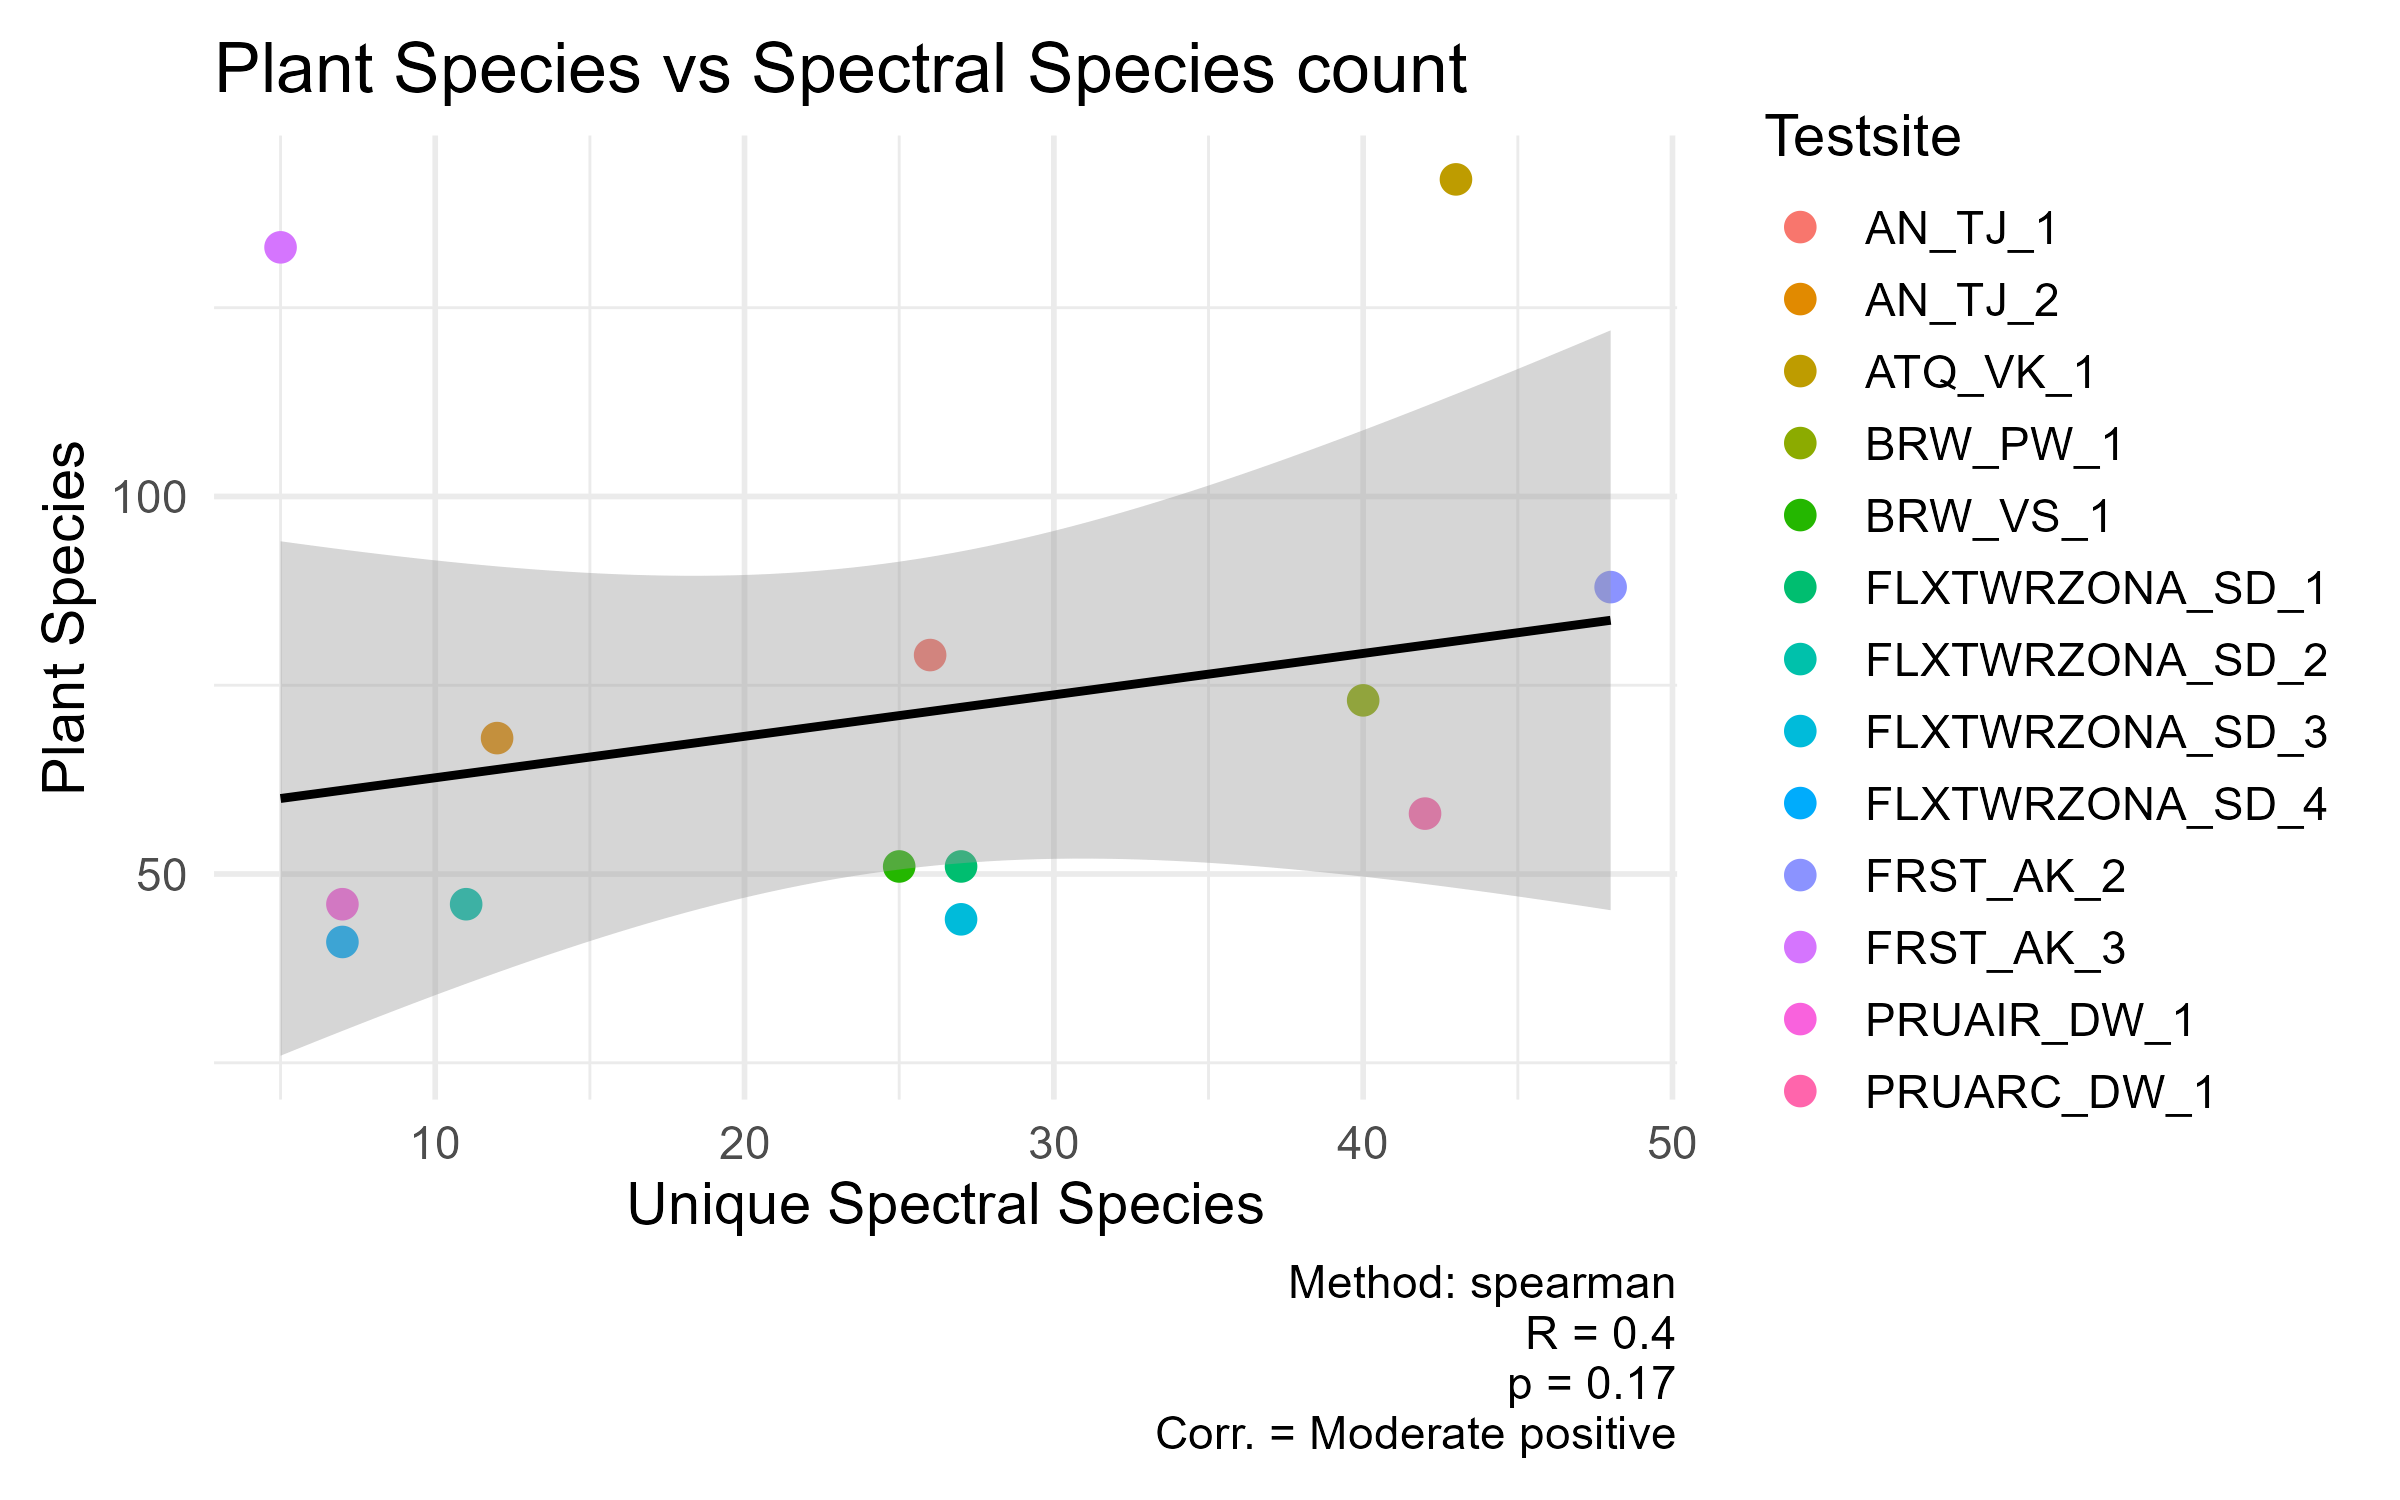
\includegraphics[width=0.9\textwidth]{Figures/WCSS_correlation_plant_species.png} % Replace with your actual image path
    \caption{The Spearman correlation test over all test sites shows a moderate positive correlation between spectral species and plant species with an $R$ value of 0.4 and a $p$-value of 0.17.}
    \label{fig:WCSS_correlation_plant_species}
\end{figure}

\begin{table}[ht]
\centering
\caption{Summary of linear regression model predicting plant species richness from spectral species richness over all test sites}
\begin{tabular}{lcccc}
\hline
\textbf{Predictor} & \textbf{Estimate} & \textbf{Std. Error} & \textbf{t value} & \textbf{Pr($>$$|$t$|$)} \\
\hline
Intercept & 57.2577 & 18.1108 & 3.162 & \textbf{0.00905**} \\
Unique Spectral Species & 0.5489 & 0.6323 & 0.868 & 0.40390 \\
\hline
\multicolumn{5}{l}{\textit{Residual standard error:} 33.38 on 11 degrees of freedom} \\
\multicolumn{5}{l}{\textit{Multiple R-squared:} 0.06411 \quad \textit{Adjusted R-squared:} -0.02097} \\
\multicolumn{5}{l}{\textit{F-statistic:} 0.7535 on 1 and 11 DF, \quad \textit{p-value:} 0.4039} \\
\hline
\end{tabular}
\label{tab:lm_plantspecies_spectral}
\end{table}

\subsection{Results for Group C/D}
The Spearman correlation analysis for Group C/D indicated a moderate positive correlation between spectral species richness and plant species richness, with a correlation coefficient of $R$ = 0.42 (Fig. \ref{fig:WCSS_correlation_plant_species_part_c_d}). However, the linear regression model did not show a statistically significant relationship (Tab. \ref{tab:lm_plantspecies_spectral_group_cd}). The model explained only a small portion of the variance in plant species richness ($R^2$ = 0.02931), and the predictor variable was not significant ($p$ = 0.636).
\begin{figure}[H]
    \centering
    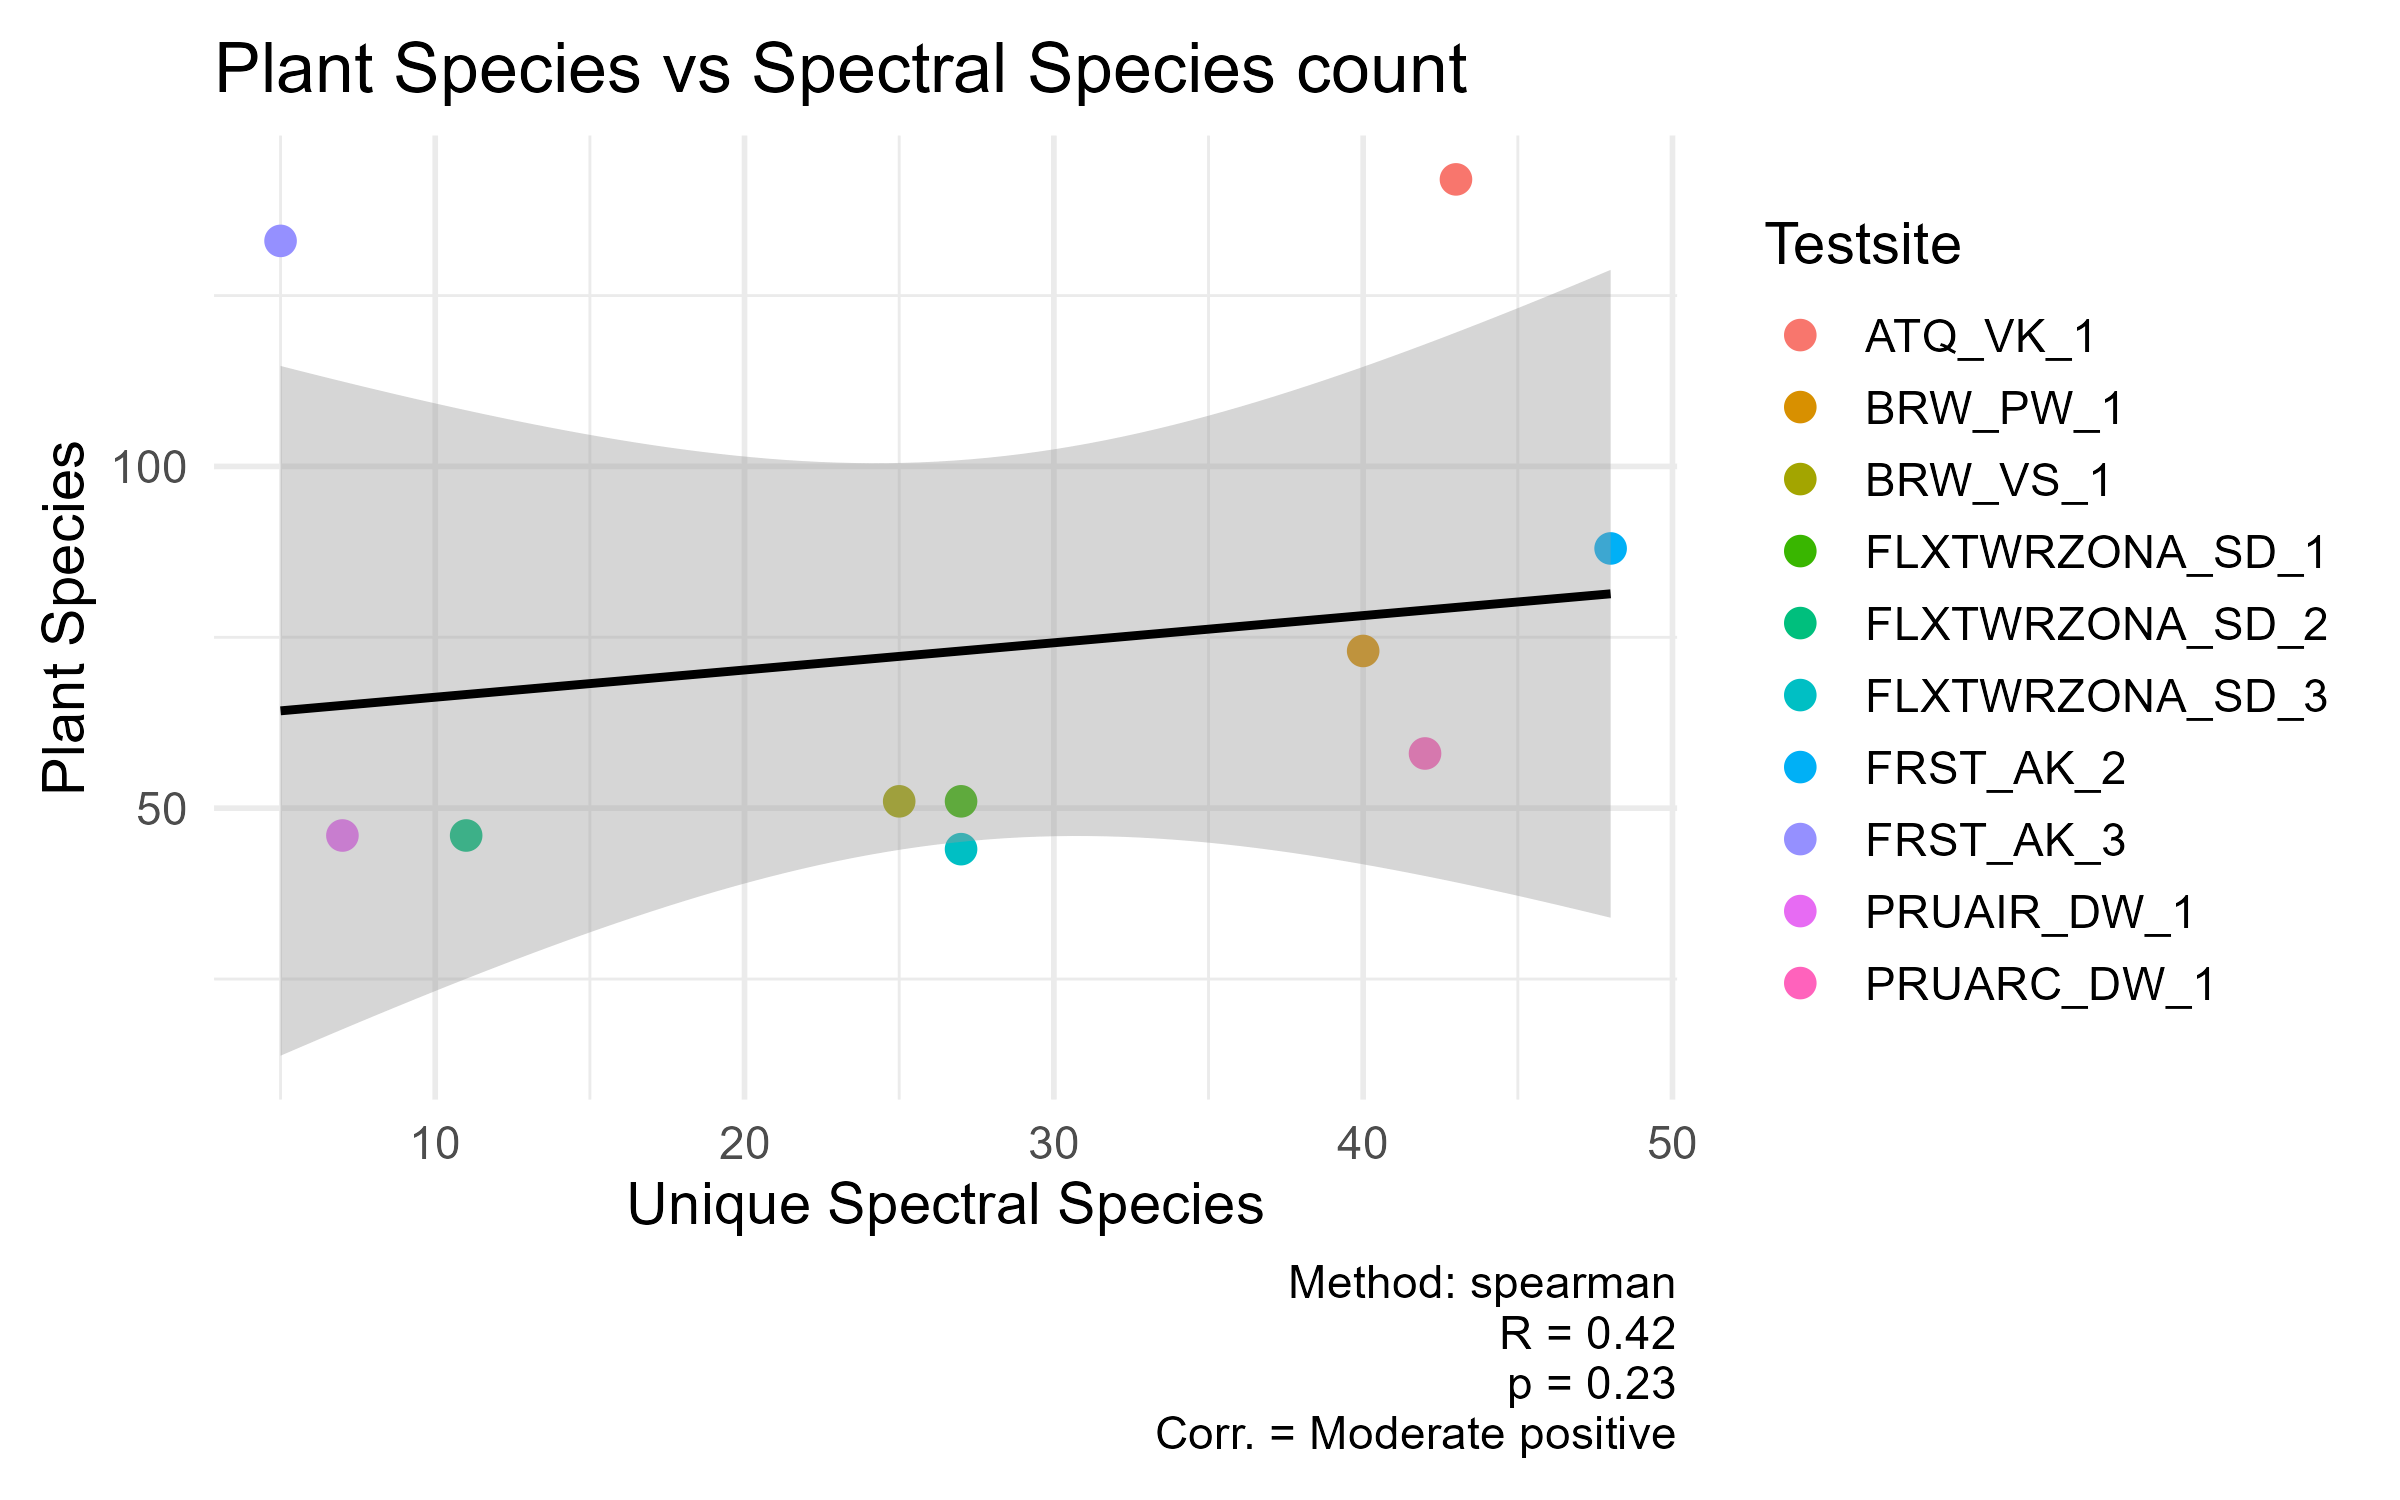
\includegraphics[width=0.9\textwidth]{Figures/WCSS_correlation_plant_species_part_c_d.png} % Replace with your actual image path
    \caption{The Spearman correlation test within Group C/D shows a moderate positive correlation between spectral species and plant species with an $R$ value of 0.42 and a $p$-value of 0.23.}
    \label{fig:WCSS_correlation_plant_species_part_c_d}
\end{figure}

\begin{table}[ht]
\centering
\caption{Summary of linear regression model predicting plant species richness from spectral species richness for Group C/D}
\begin{tabular}{lcccc}
\hline
\textbf{Predictor} & \textbf{Estimate} & \textbf{Std. Error} & \textbf{t value} & \textbf{Pr($>$$|$t$|$)} \\
\hline
Intercept & 62.2493 & 25.3566 & 2.455 & \textbf{0.0396*} \\
Unique Spectral Species & 0.3982 & 0.8102 & 0.491 & 0.6363 \\
\hline
\multicolumn{5}{l}{\textit{Residual standard error:} 38.28 on 8 degrees of freedom} \\
\multicolumn{5}{l}{\textit{Multiple R-squared:} 0.02931 \quad \textit{Adjusted R-squared:} -0.09203} \\
\multicolumn{5}{l}{\textit{F-statistic:} 0.2416 on 1 and 8 DF, \quad \textit{p-value:} 0.6363} \\
\hline
\end{tabular}
\label{tab:lm_plantspecies_spectral_group_cd}
\end{table}

\subsection{Results for Group E}
The Kendall’s tau correlation analysis for Group E indicated a very strong positive correlation between spectral species richness and plant species richness, with a correlation coefficient of $R$ = 1 (Fig. \ref{fig:WCSS_correlation_plant_species_part_e}). However, the linear regression model did not show a statistically significant relationship (Tab. \ref{tab:lm_plantspecies_spectral_group_e}). The model explained only a small portion of the variance in plant species richness ($R^2$ = 0.7656), and the predictor variable was not significant ($p$ = 0.636).
\begin{figure}[H]
    \centering
    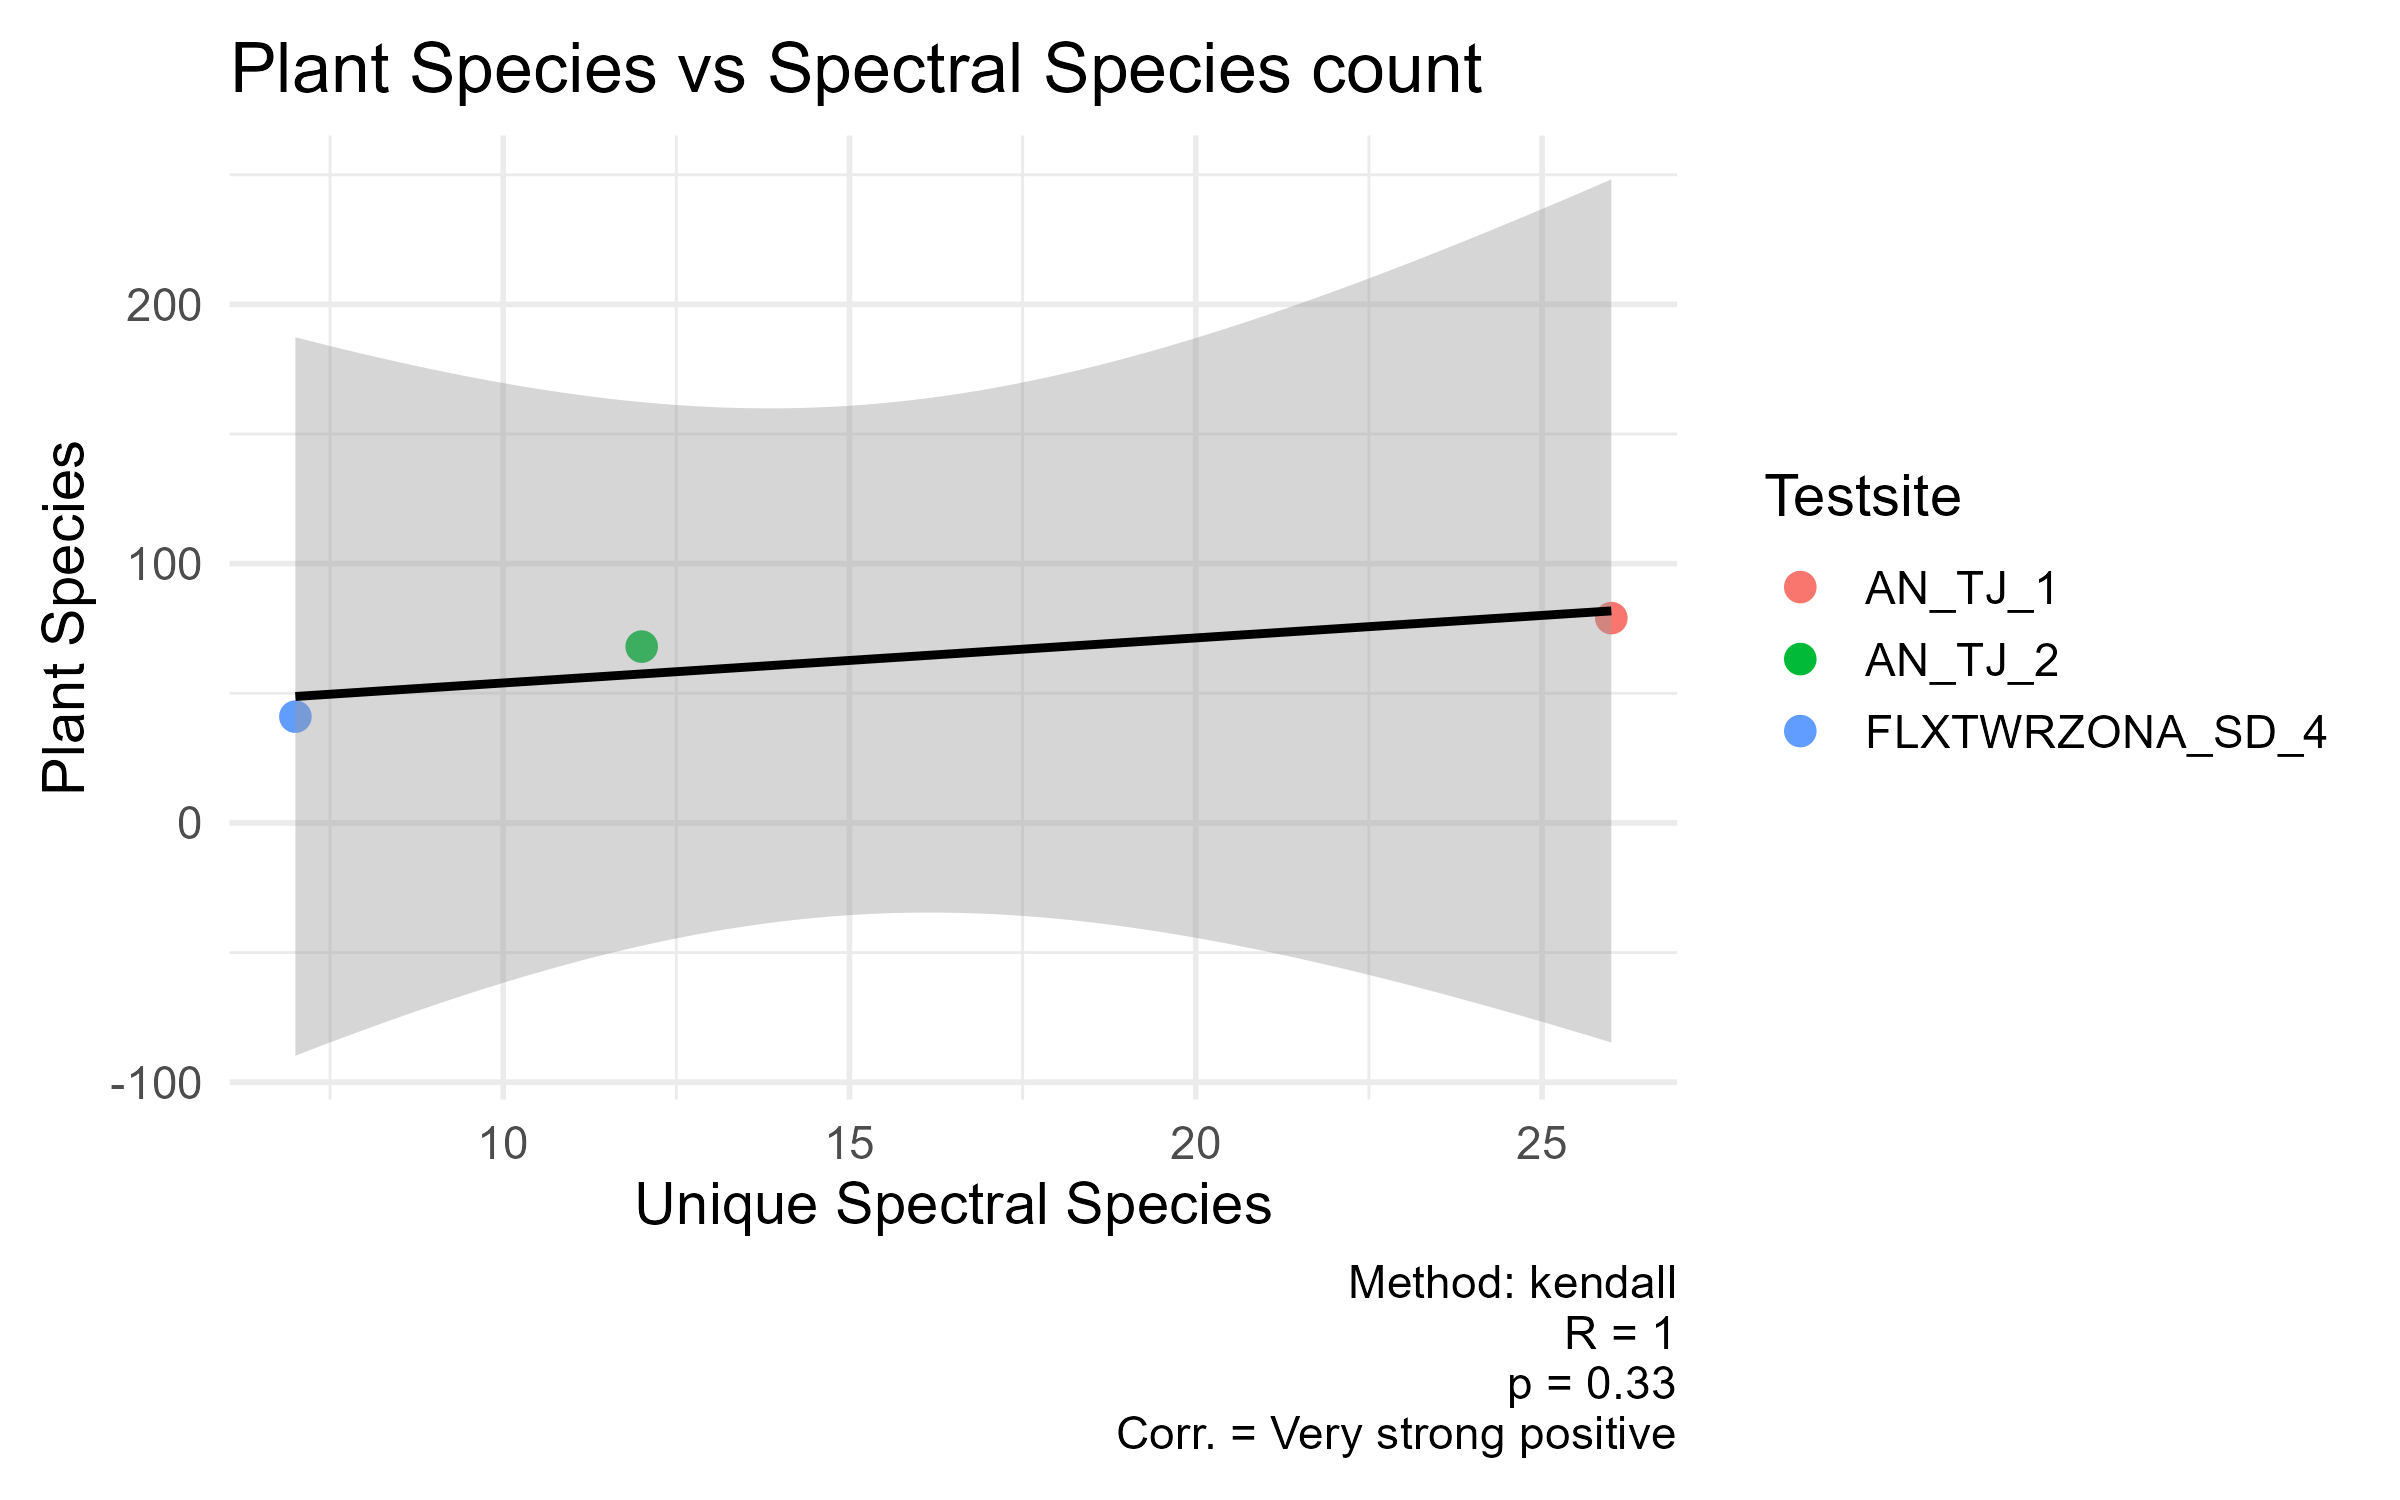
\includegraphics[width=0.9\textwidth]{Figures/WCSS_correlation_plant_species_part_e.png} % Replace with your actual image path
    \caption{The Kendall’s tau correlation test within Group E shows a very strong positive correlation between spectral species and plant species with an $R$ value of 1 and a $p$-value of 0.33.}
    \label{fig:WCSS_correlation_plant_species_part_e}
\end{figure}

\begin{table}[ht]
\centering
\caption{Summary of linear regression model predicting plant species richness from spectral species richness for Group E}
\begin{tabular}{lcccc}
\hline
\textbf{Predictor} & \textbf{Estimate} & \textbf{Std. Error} & \textbf{t value} & \textbf{Pr($>$$|$t$|$)} \\
\hline
Intercept & 36.6100 & 16.3602 & 2.238 &  0.268 \\
Unique Spectral Species & 1.7371 & 0.9613 & 1.807 & 0.322 \\
\hline
\multicolumn{5}{l}{\textit{Residual standard error:} 13.39 on 1 degrees of freedom} \\
\multicolumn{5}{l}{\textit{Multiple R-squared:} 0.7656 \quad \textit{Adjusted R-squared:} 0.5311} \\
\multicolumn{5}{l}{\textit{F-statistic:} 3.266 on 1 and 1 DF, \quad \textit{p-value:} 0.3218} \\
\hline
\end{tabular}
\label{tab:lm_plantspecies_spectral_group_e}
\end{table}


\section{Plant communities - spectral species}
\subsection{Results over all test sites}
The Pearson correlation analysis over all test sites indicated a negligible correlation between spectral species richness and plant community richness, with a correlation coefficient of $R$ = -0.08 (Fig. \ref{fig:WCSS_correlation_plant_communities}).

\begin{figure}[H]
    \centering
    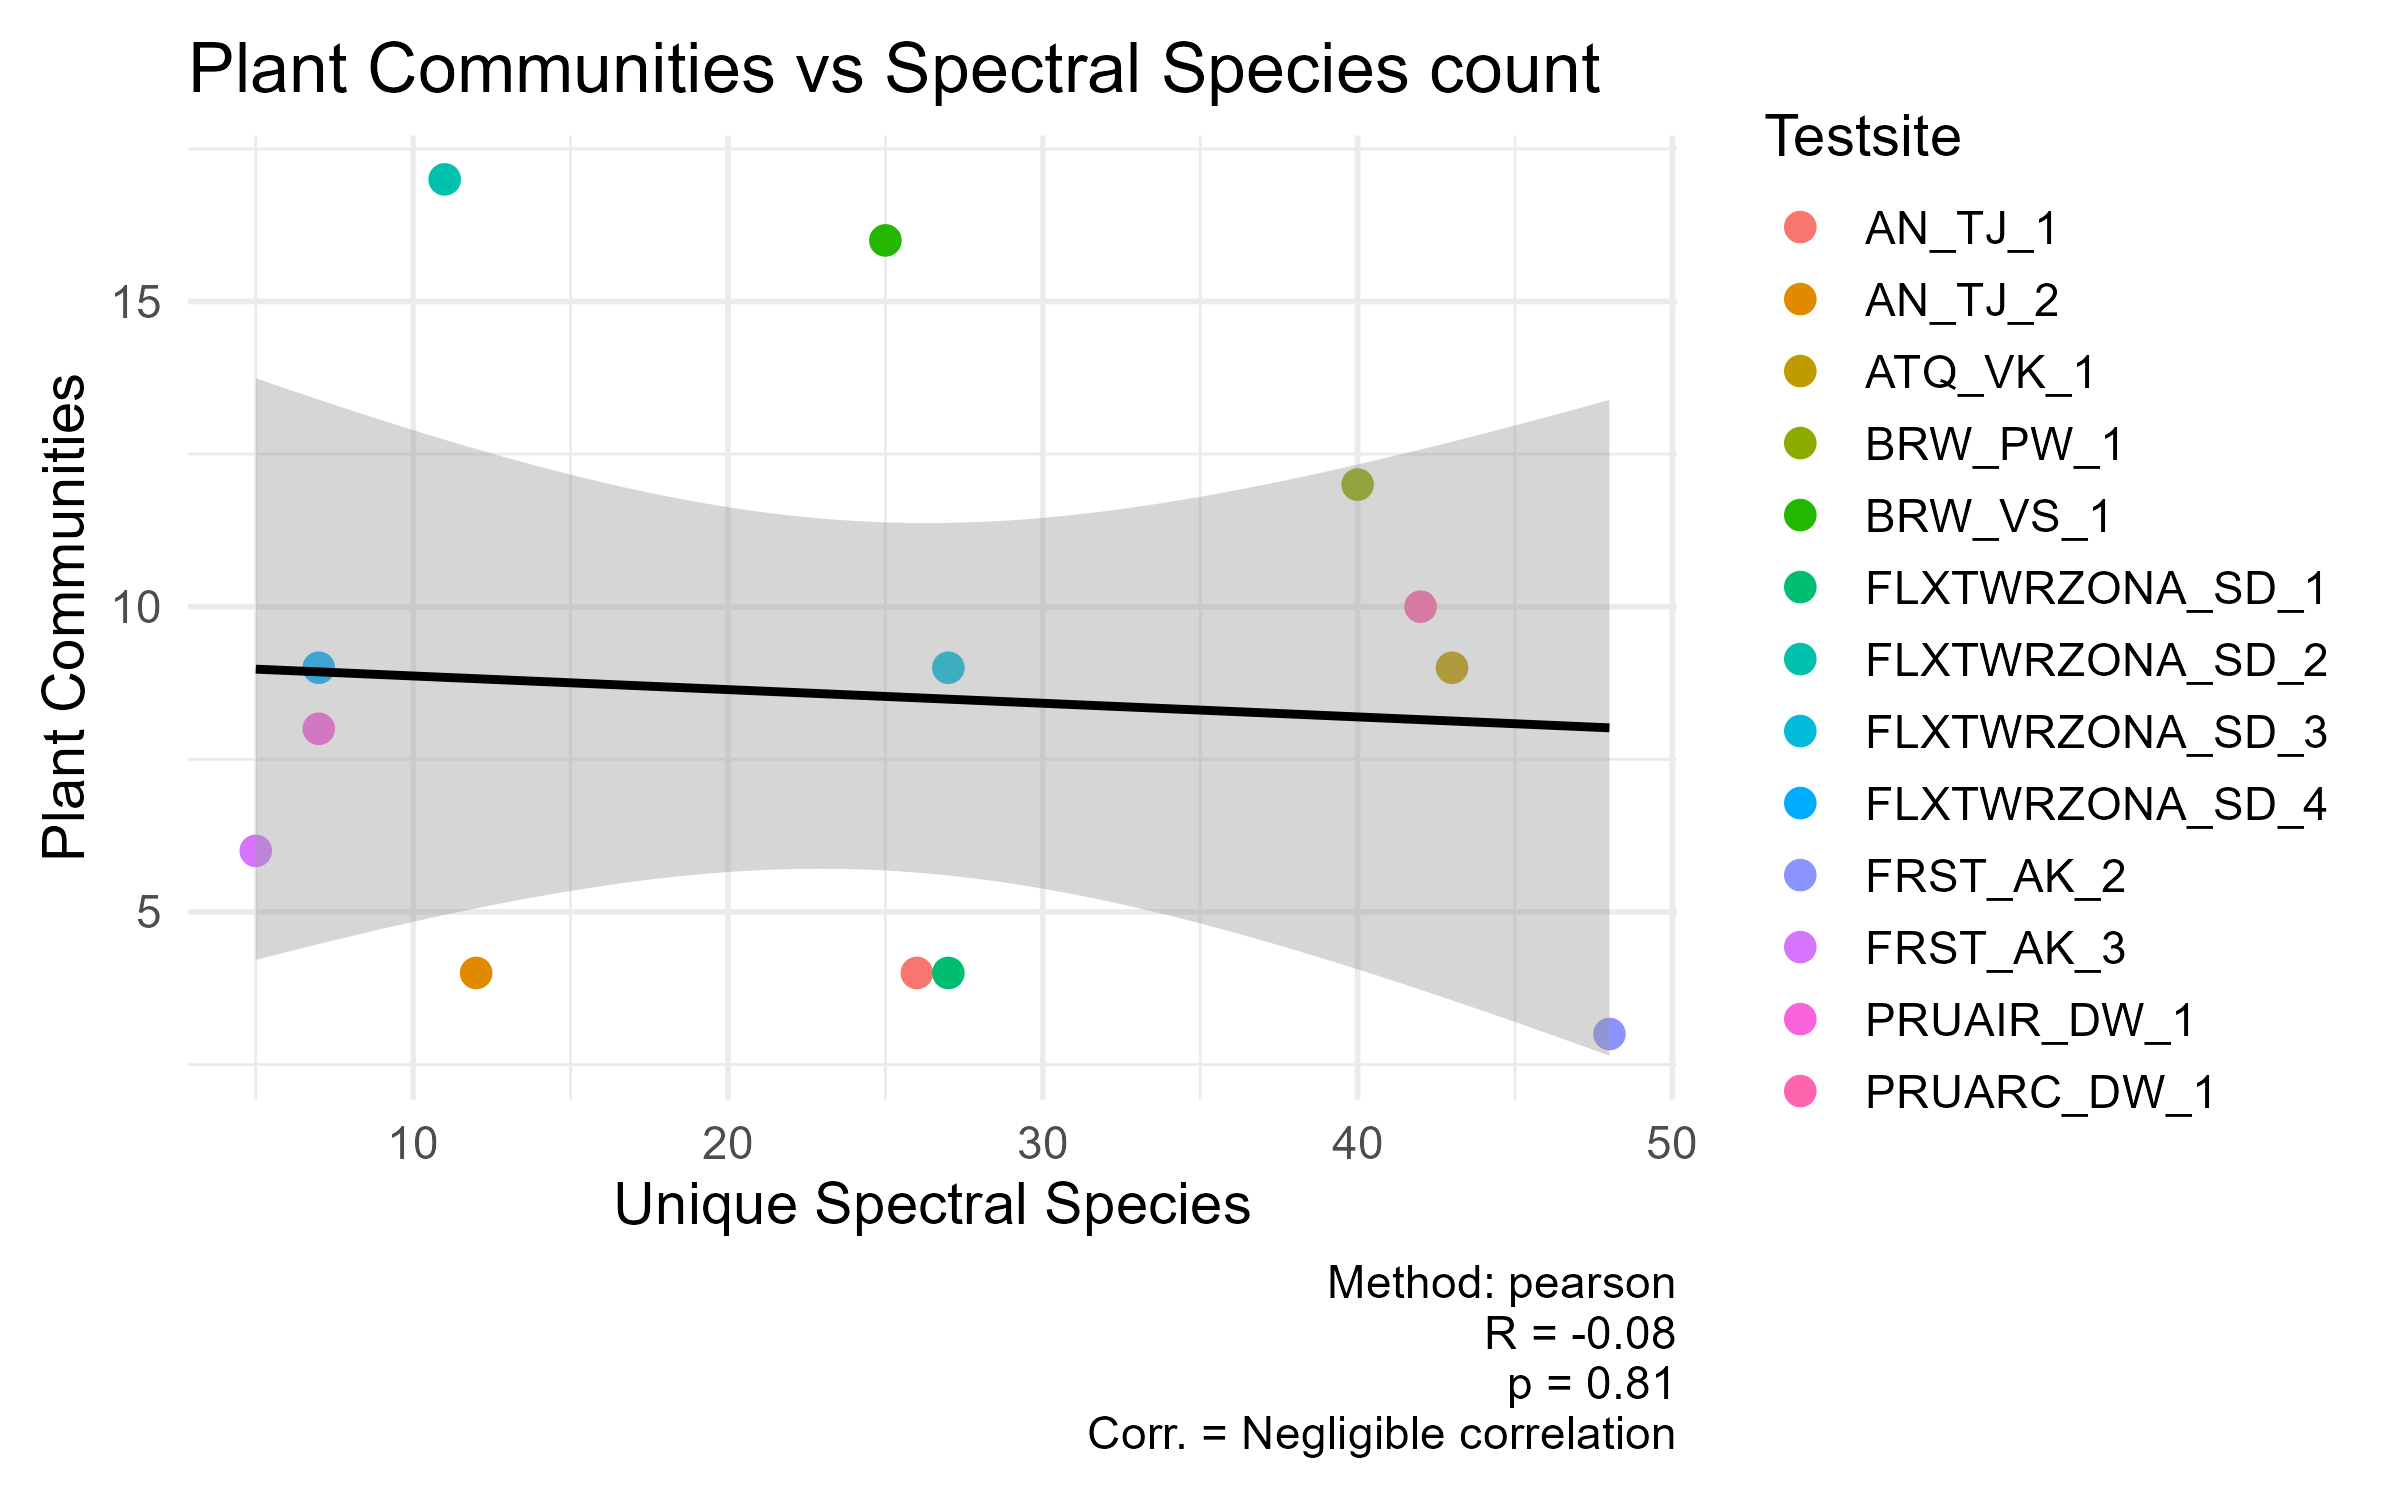
\includegraphics[width=0.9\textwidth]{Figures/WCSS_correlation_plant_communities.png} % Replace with your actual image path
    \caption{The Pearson correlation test over all test sites shows a negligible correlation between spectral species and plant communities with an $R$ value of -0.08 and a $p$-value of 0.81.}
    \label{fig:WCSS_correlation_plant_communities}
\end{figure}

\begin{table}[ht]
\centering
\caption{Summary of linear regression model predicting plant community richness from spectral species richness over all test sites}
\begin{tabular}{lcccc}
\hline
\textbf{Predictor} & \textbf{Estimate} & \textbf{Std. Error} & \textbf{t value} & \textbf{Pr($>$$|$t$|$)} \\
\hline
Intercept & 9.08876 & 2.53324 & 3.588 & \textbf{0.00426**} \\
Unique Spectral Species & -0.02236 & 0.08845 & -0.253 & 0.80512 \\
\hline
\multicolumn{5}{l}{\textit{Residual standard error:} 4.669 on 11 degrees of freedom} \\
\multicolumn{5}{l}{\textit{Multiple R-squared:} 0.005774 \quad \textit{Adjusted R-squared:} -0.08461} \\
\multicolumn{5}{l}{\textit{F-statistic:} 0.06389 on 1 and 11 DF, \quad \textit{p-value:} 0.8051} \\
\hline
\end{tabular}
\label{tab:lm_plant_community_spectral}
\end{table}

\subsection{Results for Group C/D}
The Pearson correlation analysis for Group C/D indicated a weak negative correlation between spectral species richness and plant community richness, with a correlation coefficient of $R$ = -0.2 (Fig. \ref{fig:WCSS_correlation_plant_communities_part_c_d}).
\begin{figure}[H]
    \centering
    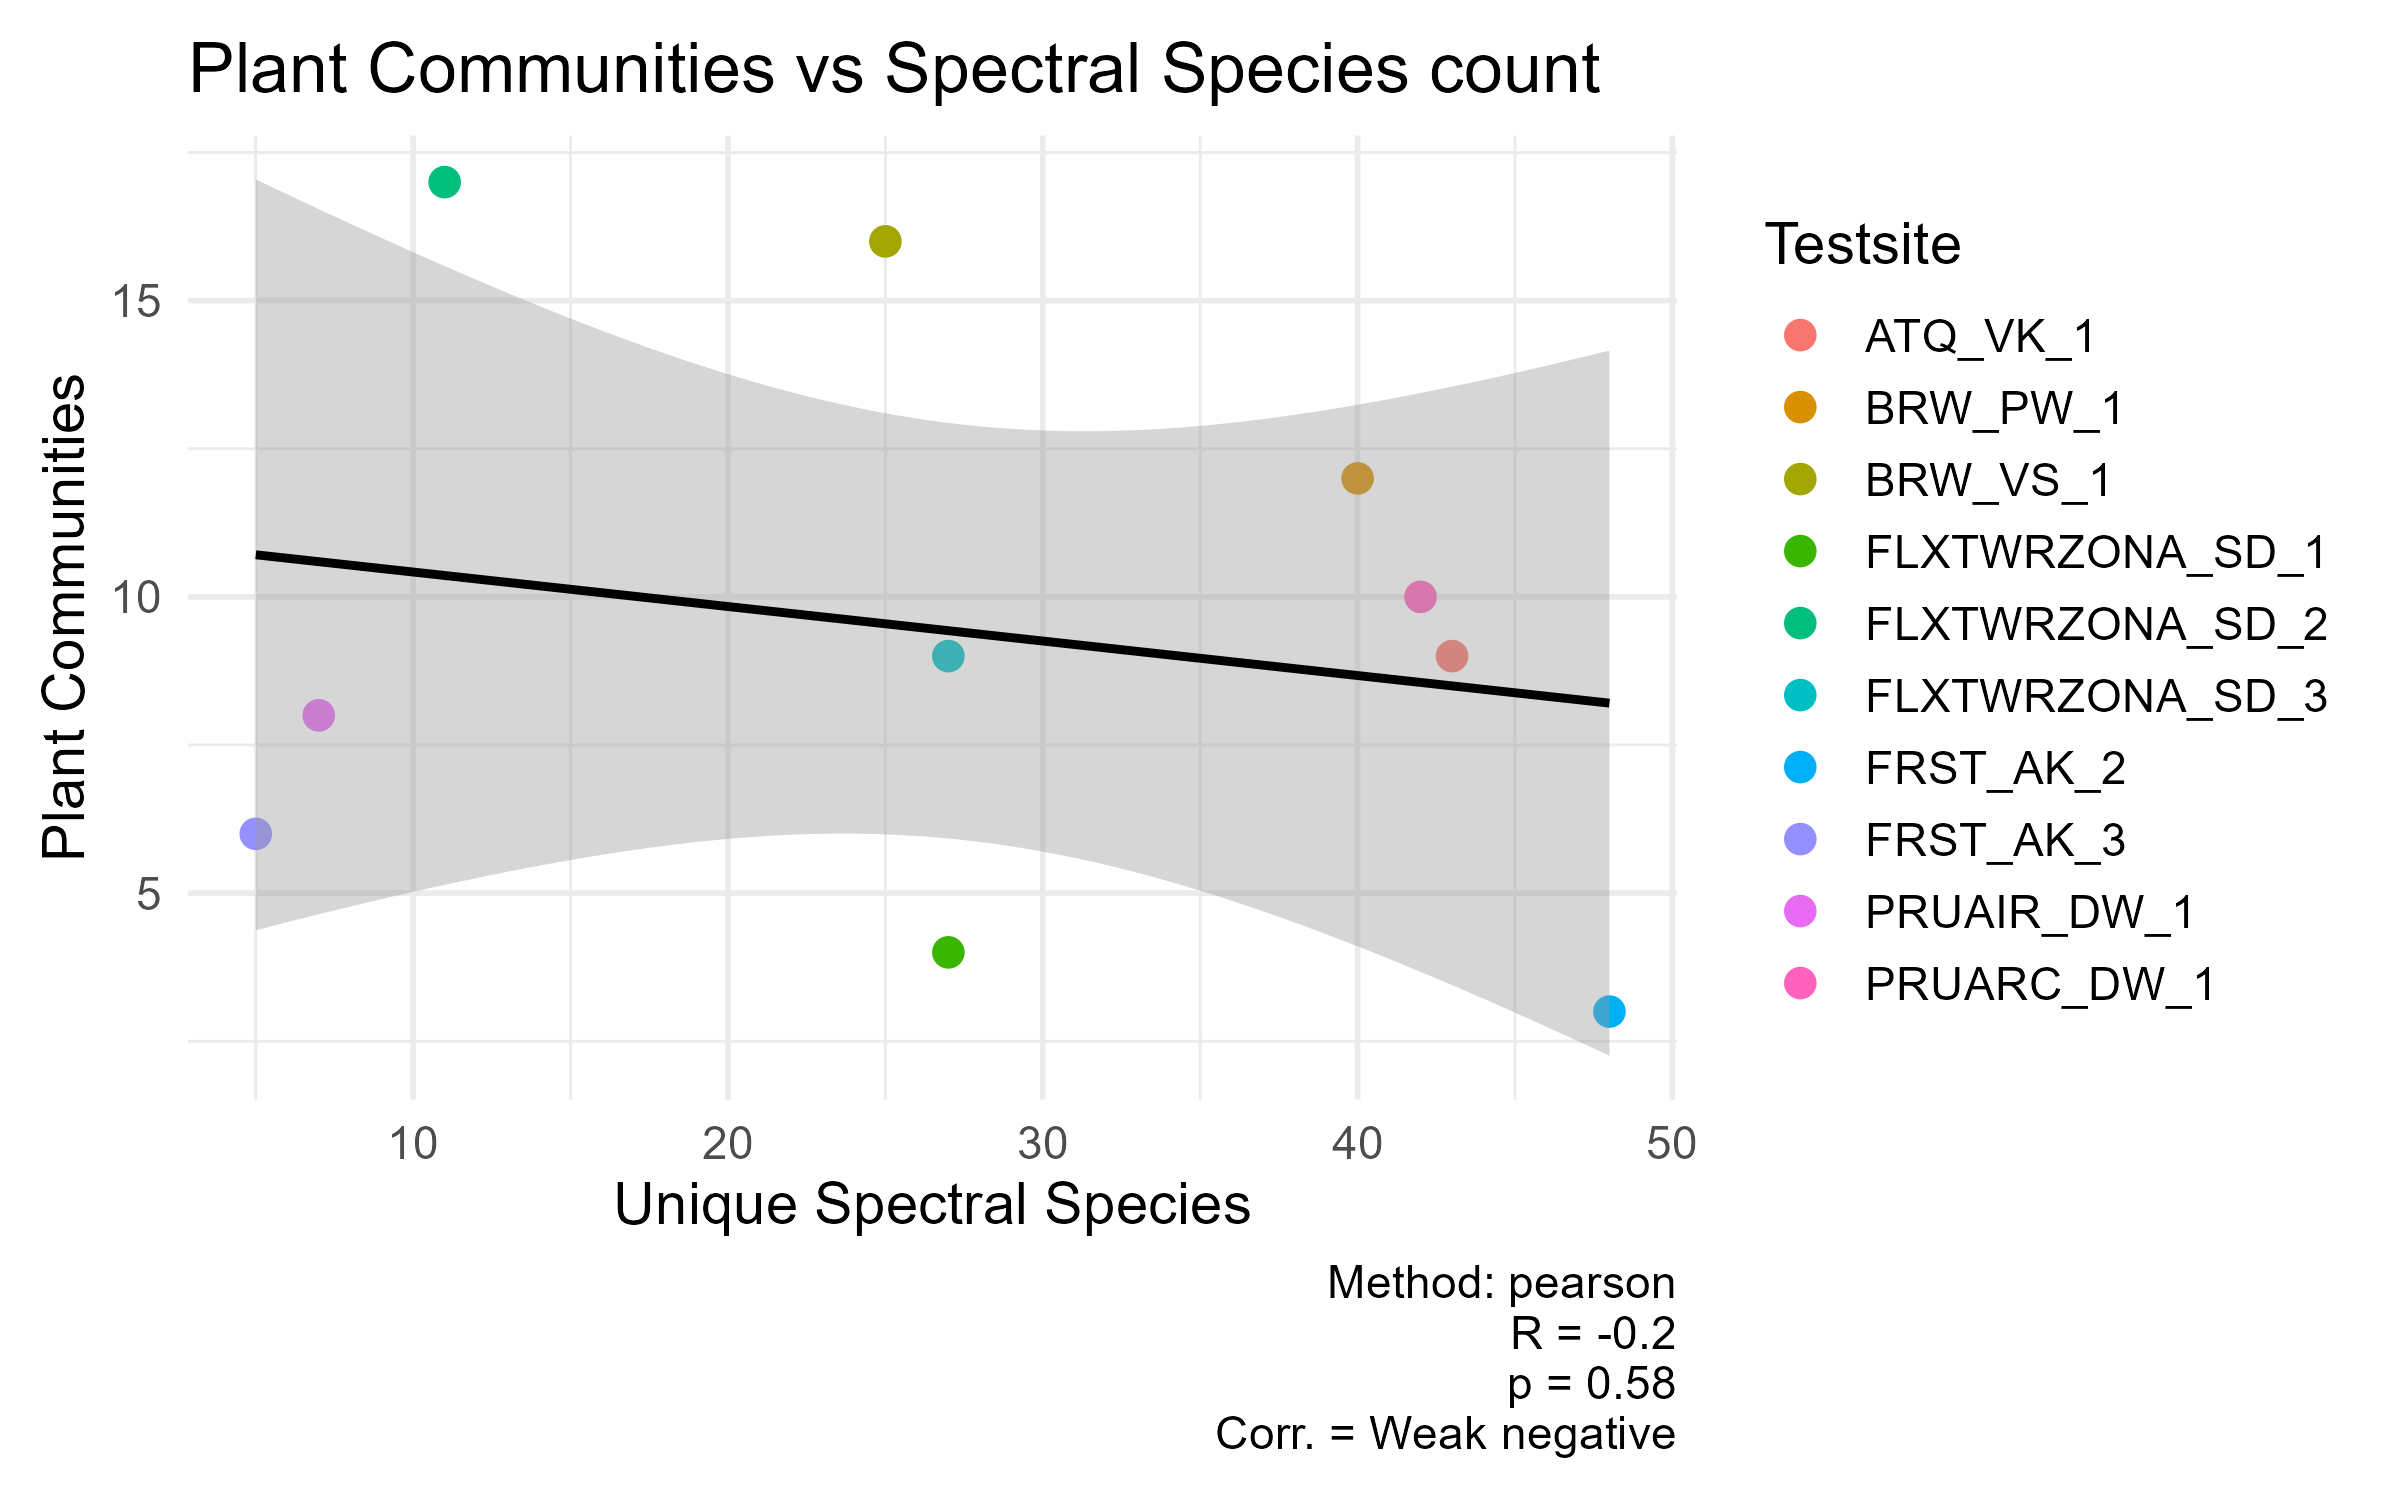
\includegraphics[width=0.9\textwidth]{Figures/WCSS_correlation_plant_communities_part_c_d.png} % Replace with your actual image path
    \caption{The Pearson correlation test within Group C/D shows a weak negative correlation between spectral species and plant communities with an $R$ value of -0.2 and a $p$-value of 0.58.}
    \label{fig:WCSS_correlation_plant_communities_part_c_d}
\end{figure}

\begin{table}[ht]
\centering
\caption{Summary of linear regression model predicting plant community richness from spectral species richness for Group C/D}
\begin{tabular}{lcccc}
\hline
\textbf{Predictor} & \textbf{Estimate} & \textbf{Std. Error} & \textbf{t value} & \textbf{Pr($>$$|$t$|$)} \\
\hline
Intercept & 11.00134 & 3.18381 & 3.455 & \textbf{0.00863**} \\
Unique Spectral Species & -0.05823 & 0.10173 & -0.572 & 0.58277 \\
\hline
\multicolumn{5}{l}{\textit{Residual standard error:} 4.807 on 8 degrees of freedom} \\
\multicolumn{5}{l}{\textit{Multiple R-squared:} 0.03935 \quad \textit{Adjusted R-squared:} -0.08074} \\
\multicolumn{5}{l}{\textit{F-statistic:} 0.3277 on 1 and 8 DF, \quad \textit{p-value:} 0.5828} \\
\hline
\end{tabular}
\label{tab:lm_plantspecies_spectral}
\end{table}


\subsection{Results for Group E}
The Pearson correlation analysis for Group E indicated a strong negative correlation between spectral species richness and plant community richness, with a correlation coefficient of $R$ = -0.82 (Fig. \ref{fig:WCSS_correlation_plant_communities_part_e}).
\begin{figure}[H]
    \centering
    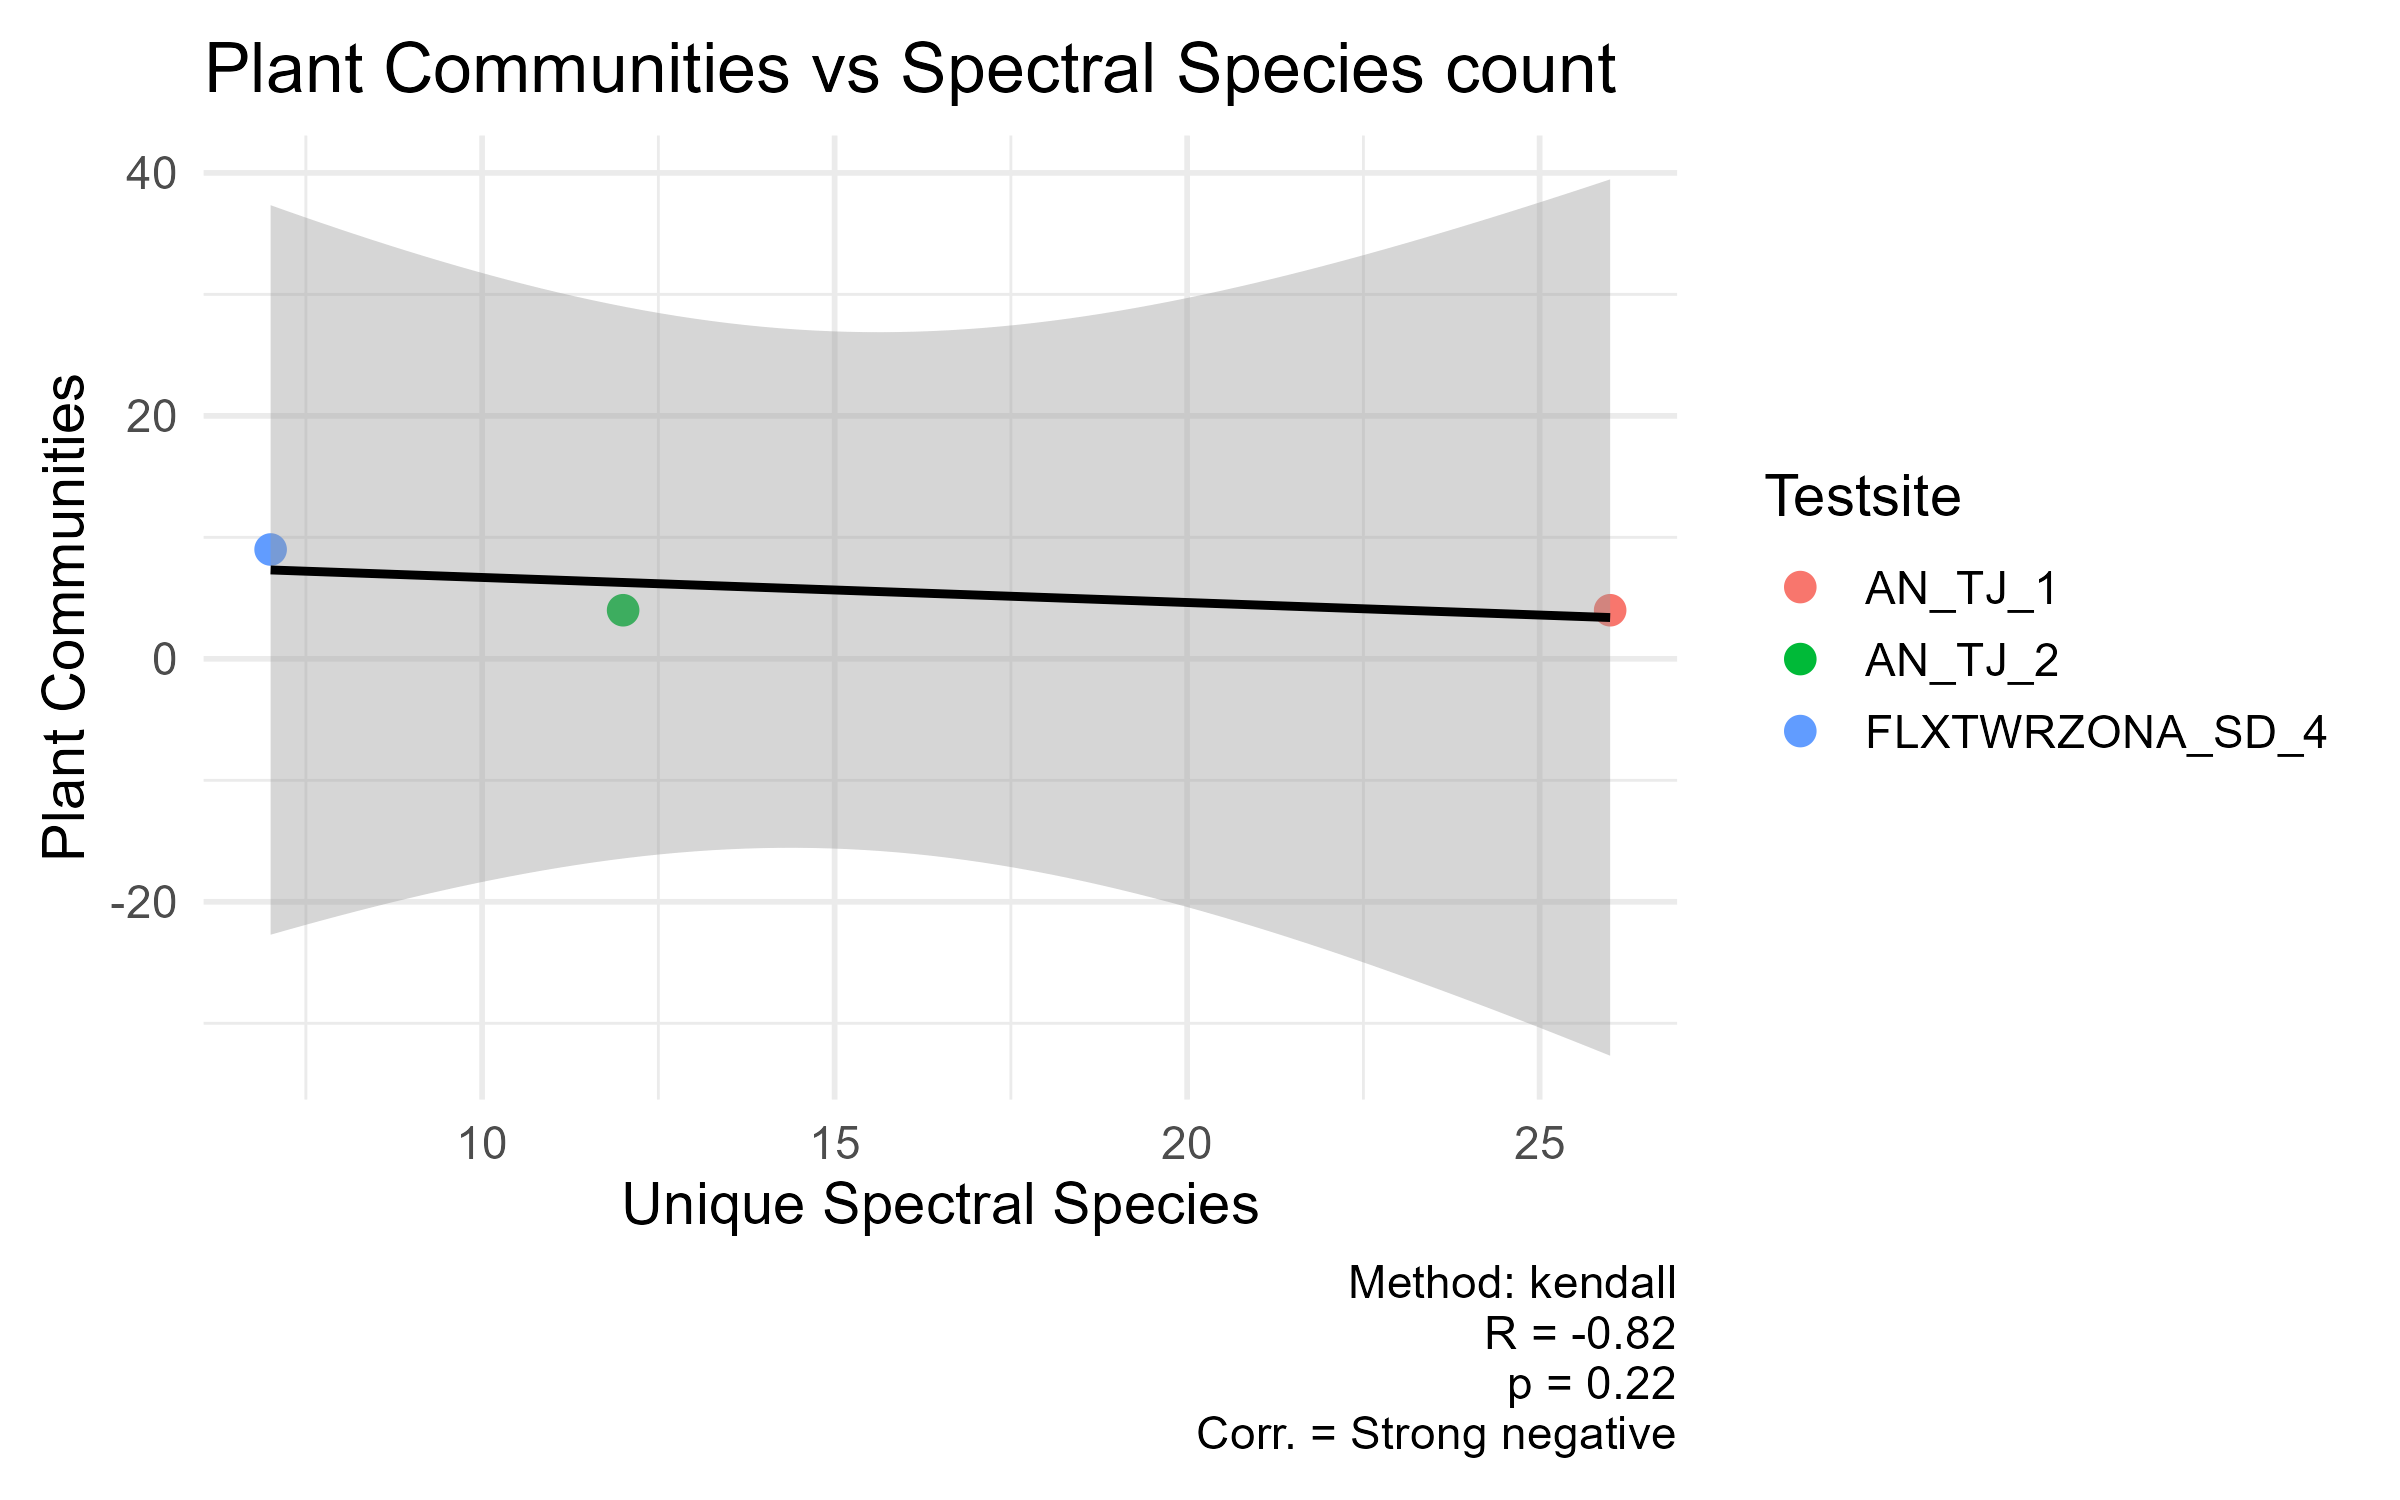
\includegraphics[width=0.9\textwidth]{Figures/WCSS_correlation_plant_communities_part_e.png} % Replace with your actual image path
    \caption{The Kendall's tau correlation test within Group E shows a strong negative correlation between spectral species and plant communities with an $R$ value of -0.82 and a $p$-value of 0.22.}
    \label{fig:WCSS_correlation_plant_communities_part_e}
\end{figure}

\begin{table}[ht]
\centering
\caption{Summary of linear regression model predicting plant community richness from spectral species richness for Group E}
\begin{tabular}{lcccc}
\hline
\textbf{Predictor} & \textbf{Estimate} & \textbf{Std. Error} & \textbf{t value} & \textbf{Pr($>$$|$t$|$)} \\
\hline
Intercept & 8.7595 & 3.5456 & 2.471 & 0.245 \\
Unique Spectral Species & -0.2062 & 0.2083 & -0.990 & 0.503 \\
\hline
\multicolumn{5}{l}{\textit{Residual standard error:} 2.902 on 1 degrees of freedom} \\
\multicolumn{5}{l}{\textit{Multiple R-squared:} 0.4948 \quad \textit{Adjusted R-squared:} -0.01031} \\
\multicolumn{5}{l}{\textit{F-statistic:} 0.9796 on 1 and 1 DF, \quad \textit{p-value:} 0.5033} \\
\hline
\end{tabular}
\label{tab:lm_plantspecies_spectral}
\end{table}

\section{Habitat types - spectral species}
\subsection{Results over all test sites}
The Pearson correlation analysis over all test sites indicated a weak positive correlation between spectral species richness and habitat type richness, with a correlation coefficient of $R$ = 0.29 (Fig. \ref{fig:WCSS_correlation_habitat_types}).

\begin{figure}[H]
    \centering
    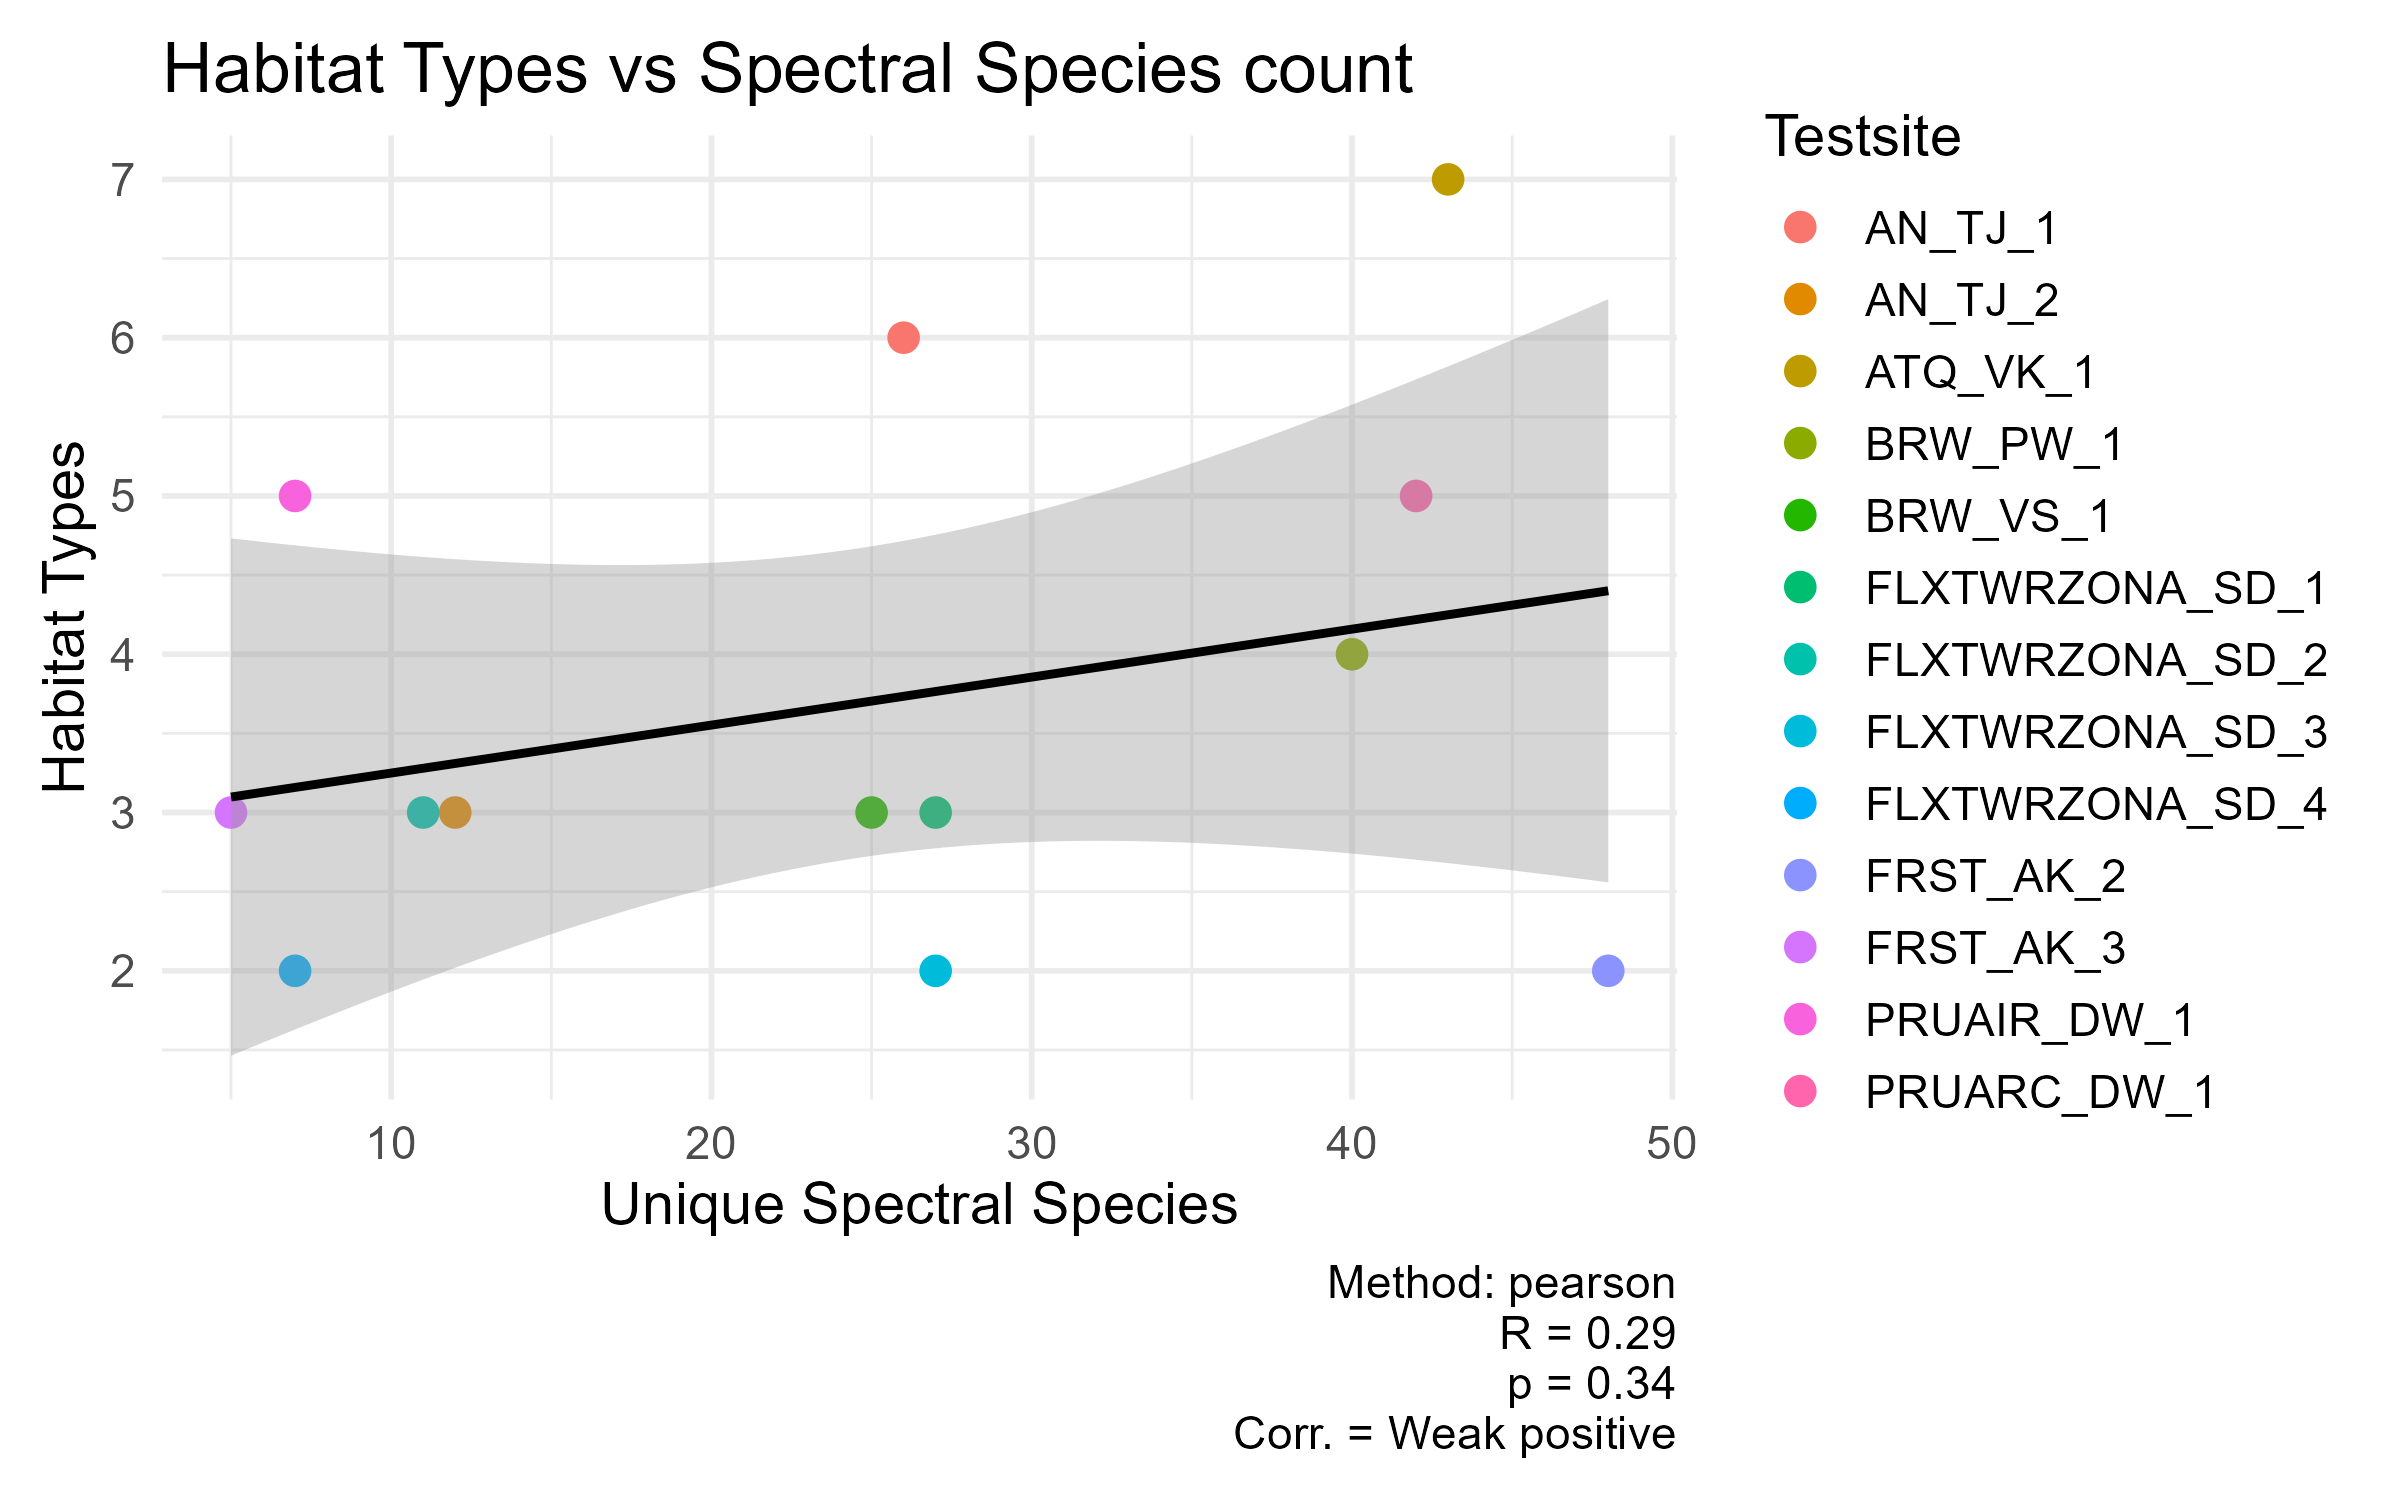
\includegraphics[width=0.9\textwidth]{Figures/WCSS_correlation_habitat_types.png} % Replace with your actual image path
    \caption{The Pearson correlation test over all test sites shows a weak positive correlation between spectral species and habitat type with an $R$ value of 0.29 and a $p$-value of 0.34.}
    \label{fig:WCSS_correlation_habitat_types}
\end{figure}

\begin{table}[ht]
\centering
\caption{Summary of linear regression model predicting habitat type richness from spectral species richness over all test sites}
\begin{tabular}{lcccc}
\hline
\textbf{Predictor} & \textbf{Estimate} & \textbf{Std. Error} & \textbf{t value} & \textbf{Pr($>$$|$t$|$)} \\
\hline
Intercept & 2.94635 & 0.86879 & 3.391 & \textbf{0.00602**} \\
Unique Spectral Species & 0.03030 & 0.03033 & 0.999 & 0.33925 \\
\hline
\multicolumn{5}{l}{\textit{Residual standard error:} 1.601 on 11 degrees of freedom} \\
\multicolumn{5}{l}{\textit{Multiple R-squared:} 0.08319 \quad \textit{Adjusted R-squared:} -0.0001603} \\
\multicolumn{5}{l}{\textit{F-statistic:} 0.9981 on 1 and 11 DF, \quad \textit{p-value:} 0.3392} \\
\hline
\end{tabular}
\label{tab:lm_habitat_type_spectral}
\end{table}

\subsection{Results for Group C/D}
The Pearson correlation analysis for Group C/D indicated a weak positive correlation between spectral species richness and habitat type richness, with a correlation coefficient of $R$ = 0.19 (Fig. \ref{fig:WCSS_correlation_habitat_types_part_c_d}).

\begin{figure}[H]
    \centering
    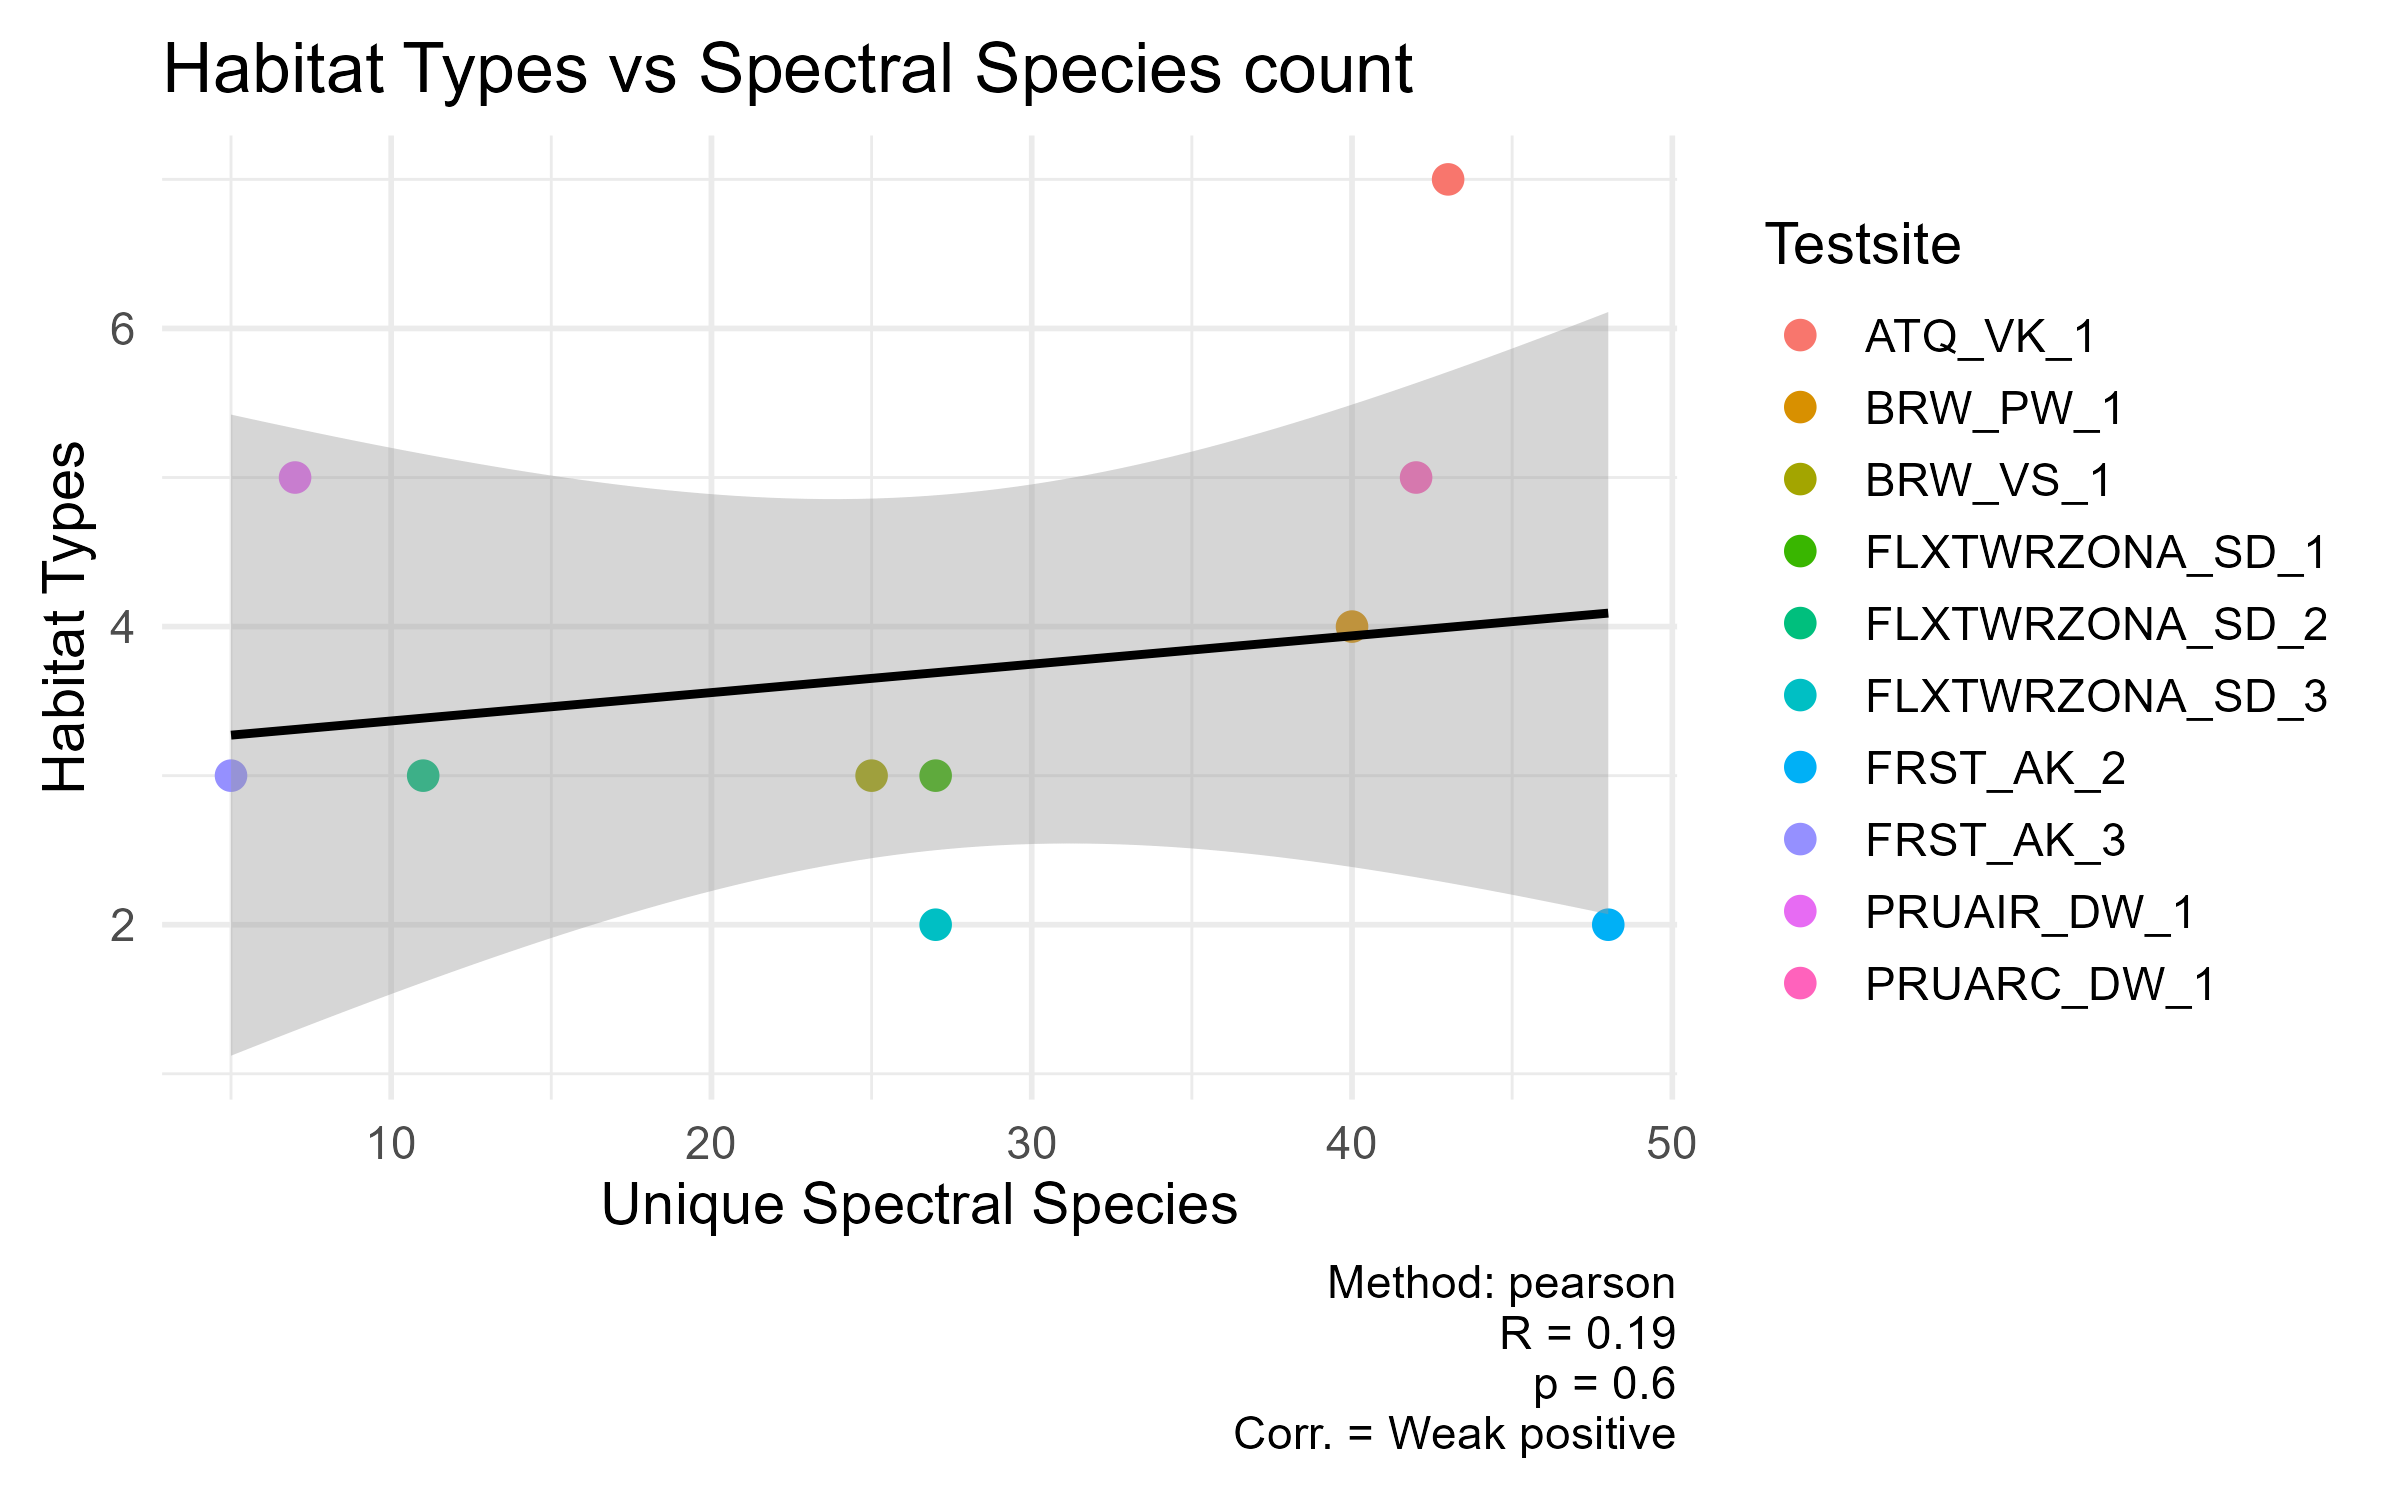
\includegraphics[width=0.9\textwidth]{Figures/WCSS_correlation_habitat_types_part_c_d.png} % Replace with your actual image path
    \caption{The Pearson correlation test within Group C/D shows a weak positive correlation between spectral species and habitat types with an $R$ value of 0.19 and a $p$-value of 0.6.}
    \label{fig:WCSS_correlation_habitat_types_part_c_d}
\end{figure}

\begin{table}[ht]
\centering
\caption{Summary of linear regression model predicting habitat type richness from spectral species richness for Group C/D}
\begin{tabular}{lcccc}
\hline
\textbf{Predictor} & \textbf{Estimate} & \textbf{Std. Error} & \textbf{t value} & \textbf{Pr($>$$|$t$|$)} \\
\hline
Intercept & 3.17648 & 1.08058 & 2.940 & \textbf{0.0187*} \\
Unique Spectral Species & 0.01904 & 0.03453 & 0.551 & 0.5964 \\
\hline
\multicolumn{5}{l}{\textit{Residual standard error:} 1.631 on 8 degrees of freedom} \\
\multicolumn{5}{l}{\textit{Multiple R-squared:} 0.03661 \quad \textit{Adjusted R-squared:} -0.08381} \\
\multicolumn{5}{l}{\textit{F-statistic:} 0.304 on 1 and 8 DF, \quad \textit{p-value:} 0.5964} \\
\hline
\end{tabular}
\label{tab:lm_plantspecies_spectral}
\end{table}


\subsection{Results for Group E}
The Pearson correlation analysis for Group E indicated a very strong positive correlation between spectral species richness and habitat type richness, with a correlation coefficient of $R$ = 1 (Fig. \ref{fig:WCSS_correlation_habitat_types_part_e}).
\begin{figure}[H]
    \centering
    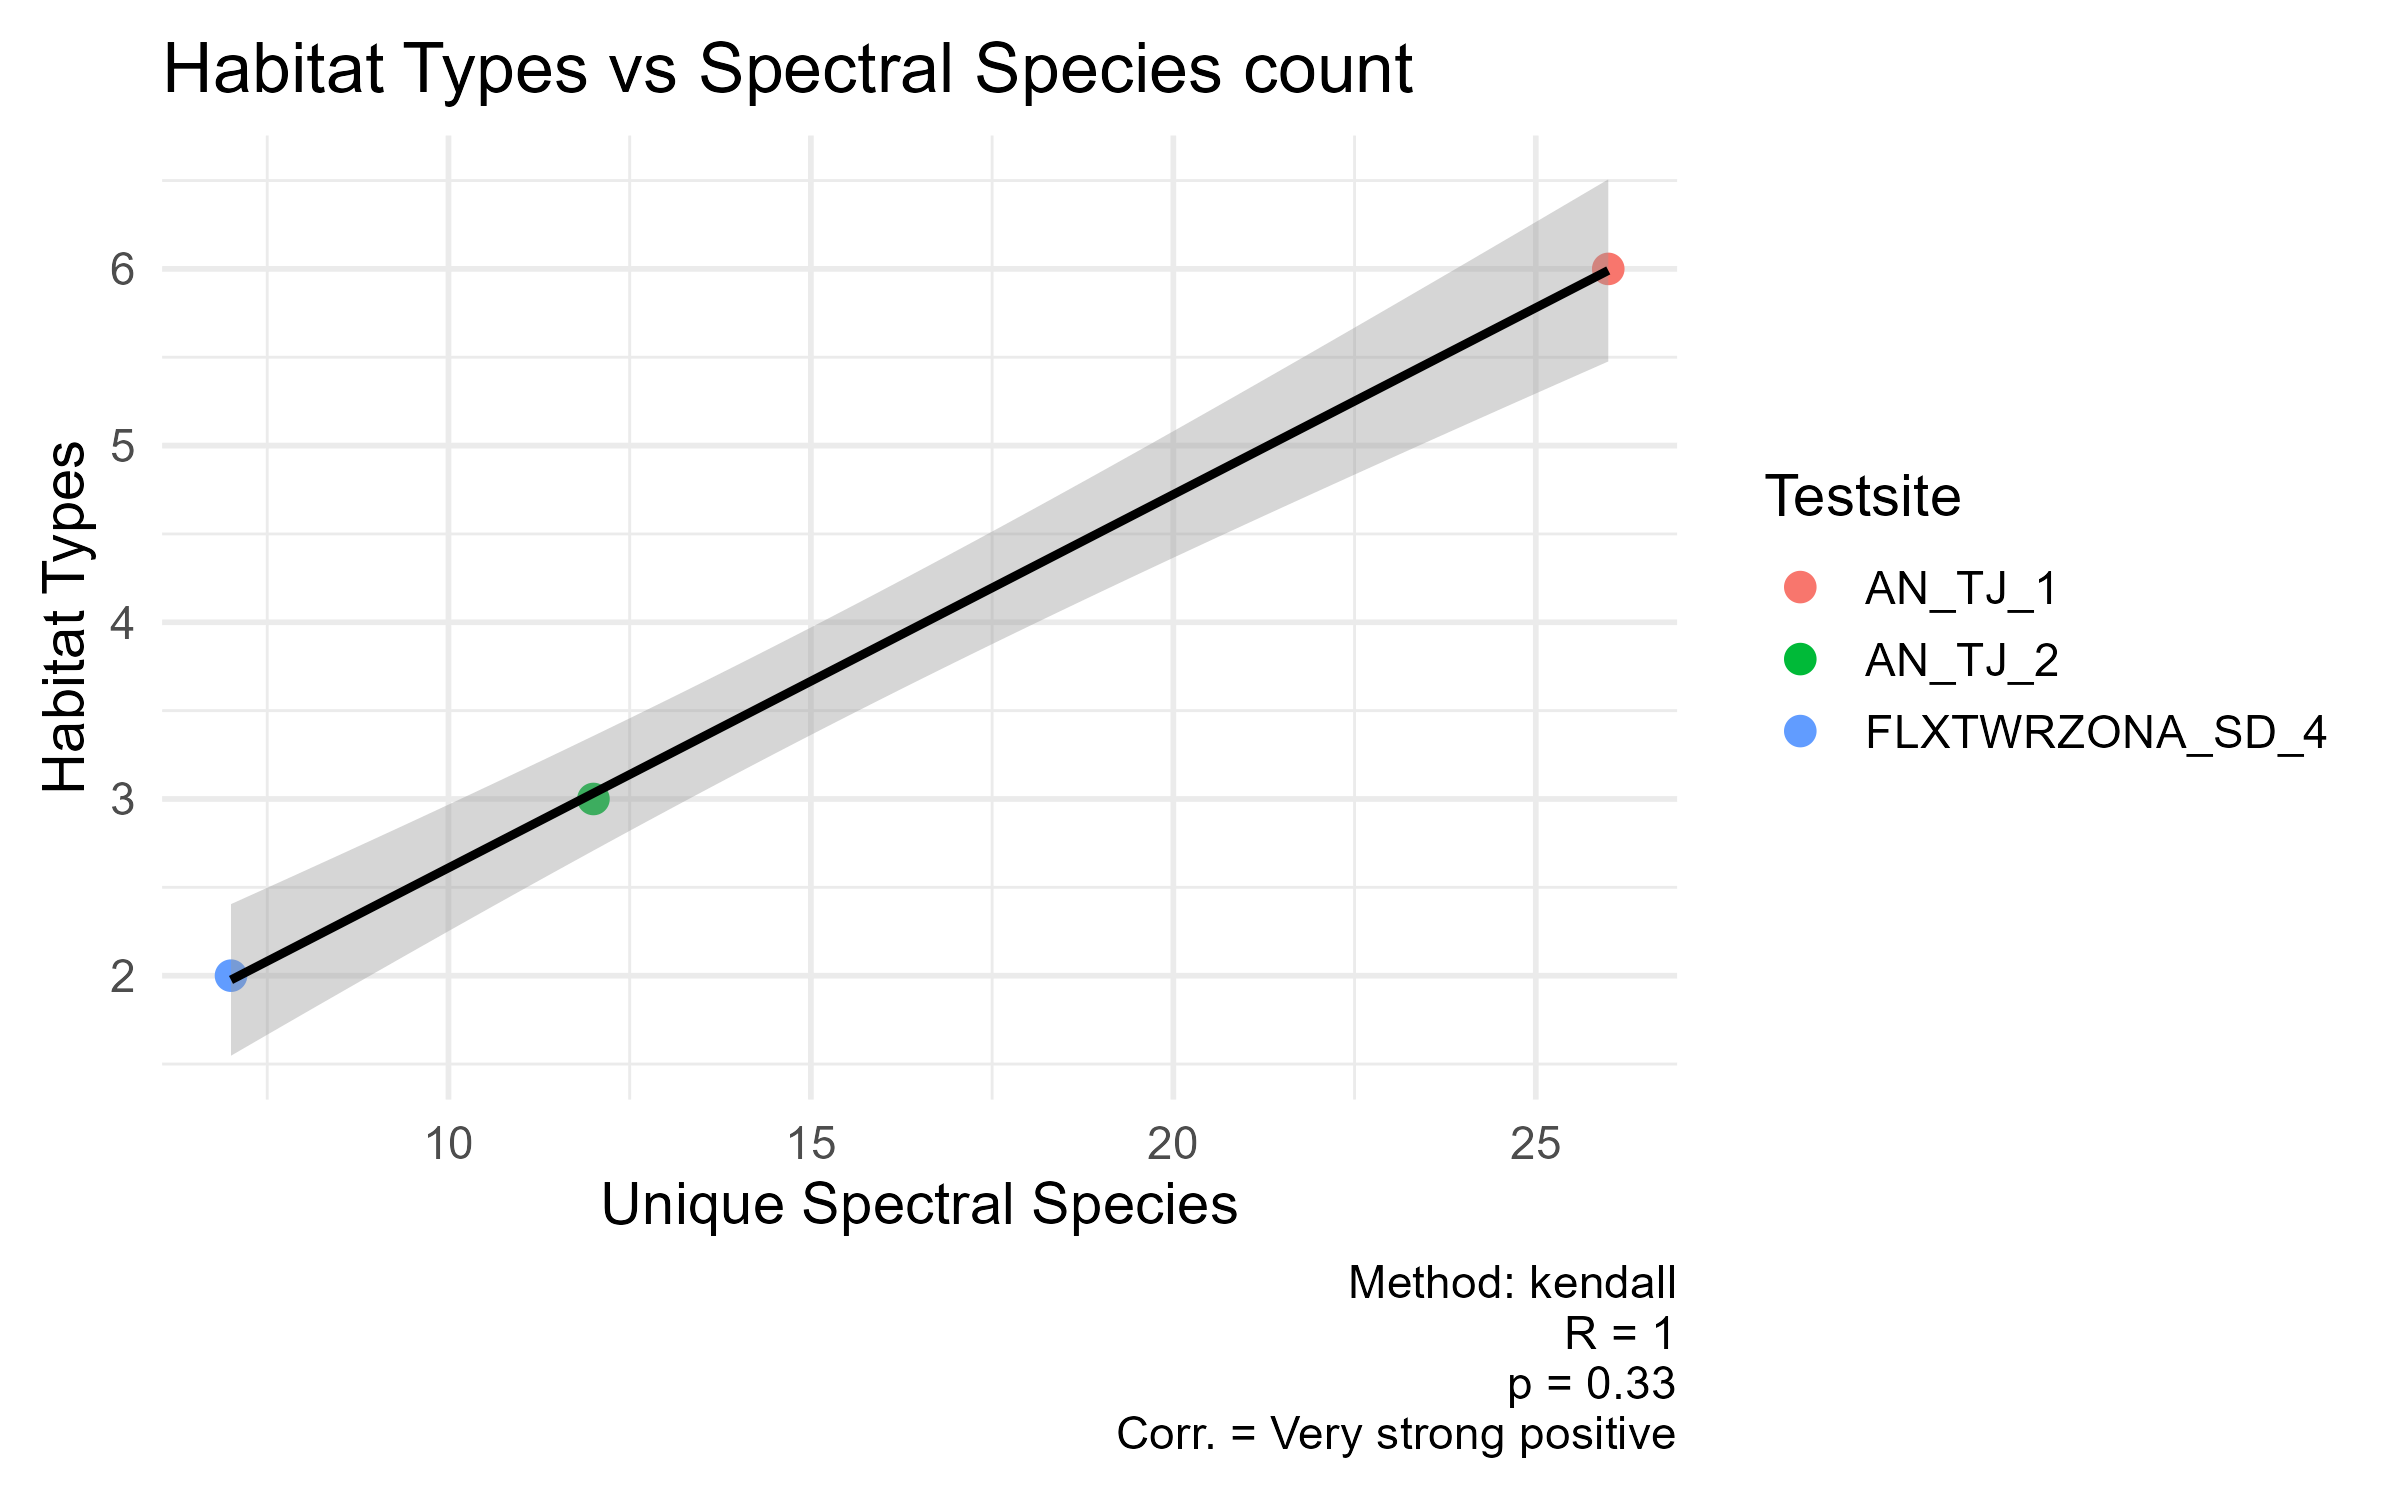
\includegraphics[width=0.9\textwidth]{Figures/WCSS_correlation_habitat_types_part_e.png} % Replace with your actual image path
    \caption{The Kendall's tau correlation test within Group E shows a very strong positive correlation between spectral species and habitat types with an $R$ value of 1 and a $p$-value of 0.33.}
    \label{fig:WCSS_correlation_habitat_types_part_e}
\end{figure}

\begin{table}[ht]
\centering
\caption{Summary of linear regression model predicting habitat type richness from spectral species richness for Group E}
\begin{tabular}{lcccc}
\hline
\textbf{Predictor} & \textbf{Estimate} & \textbf{Std. Error} & \textbf{t value} & \textbf{Pr($>$$|$t$|$)} \\
\hline
Intercept & 0.496564 & 0.050651 & 9.804 & 0.06471 \\
Unique Spectral Species & 0.211340 & 0.002976 & 71.014 & \textbf{0.00896**} \\
\hline
\multicolumn{5}{l}{\textit{Residual standard error:} 0.04145 on 1 degrees of freedom} \\
\multicolumn{5}{l}{\textit{Multiple R-squared:} 0.9998 \quad \textit{Adjusted R-squared:} 0.9996} \\
\multicolumn{5}{l}{\textit{F-statistic:} 5043 on 1 and 1 DF, \quad \textit{p-value:} 0.008964} \\
\hline
\end{tabular}
\label{tab:lm_plantspecies_spectral}
\end{table}

\section{Plot location spectral curves}
--> maybe all the plots belong into the appendix and only the result of the regression analysis is needed here?

\subsection{AN\_TJ\_1}

\begin{figure}[H]
  \centering

  \begin{subfigure}[b]{0.49\textwidth}
    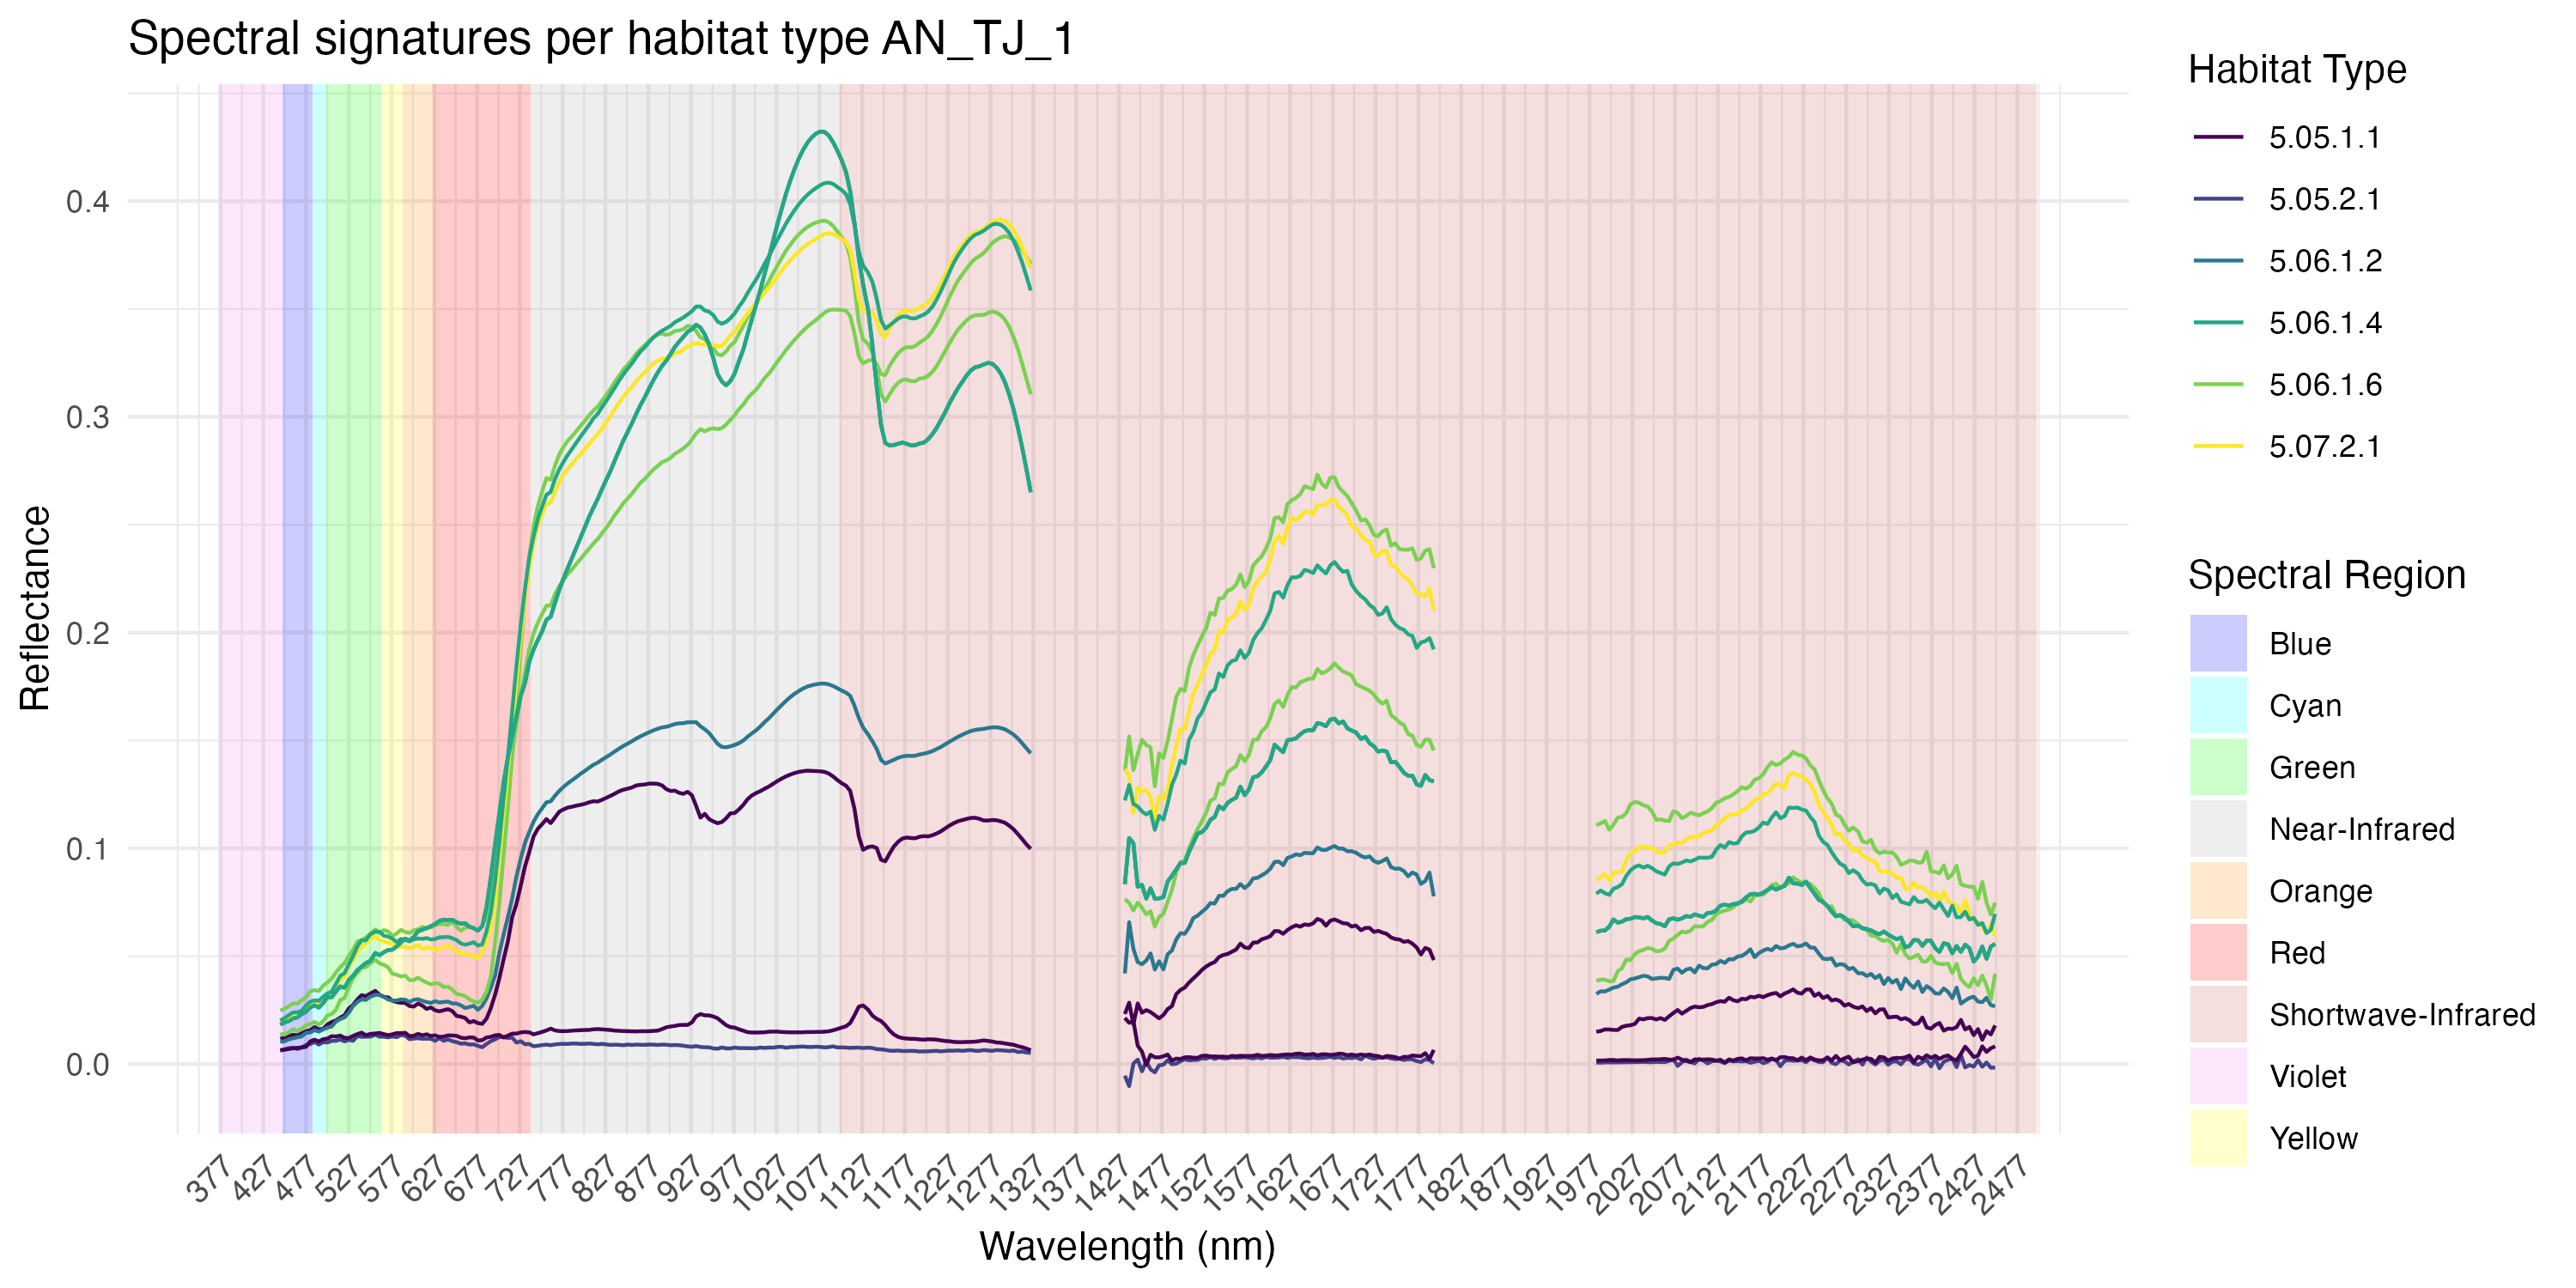
\includegraphics[width=\textwidth]{Figures/spectral_signatures/AN_TJ_1_signature_plot_habitat.png}
    \caption{}
    \label{fig:ss_ht_antj1}
  \end{subfigure}
  \hfill
  \begin{subfigure}[b]{0.49\textwidth}
    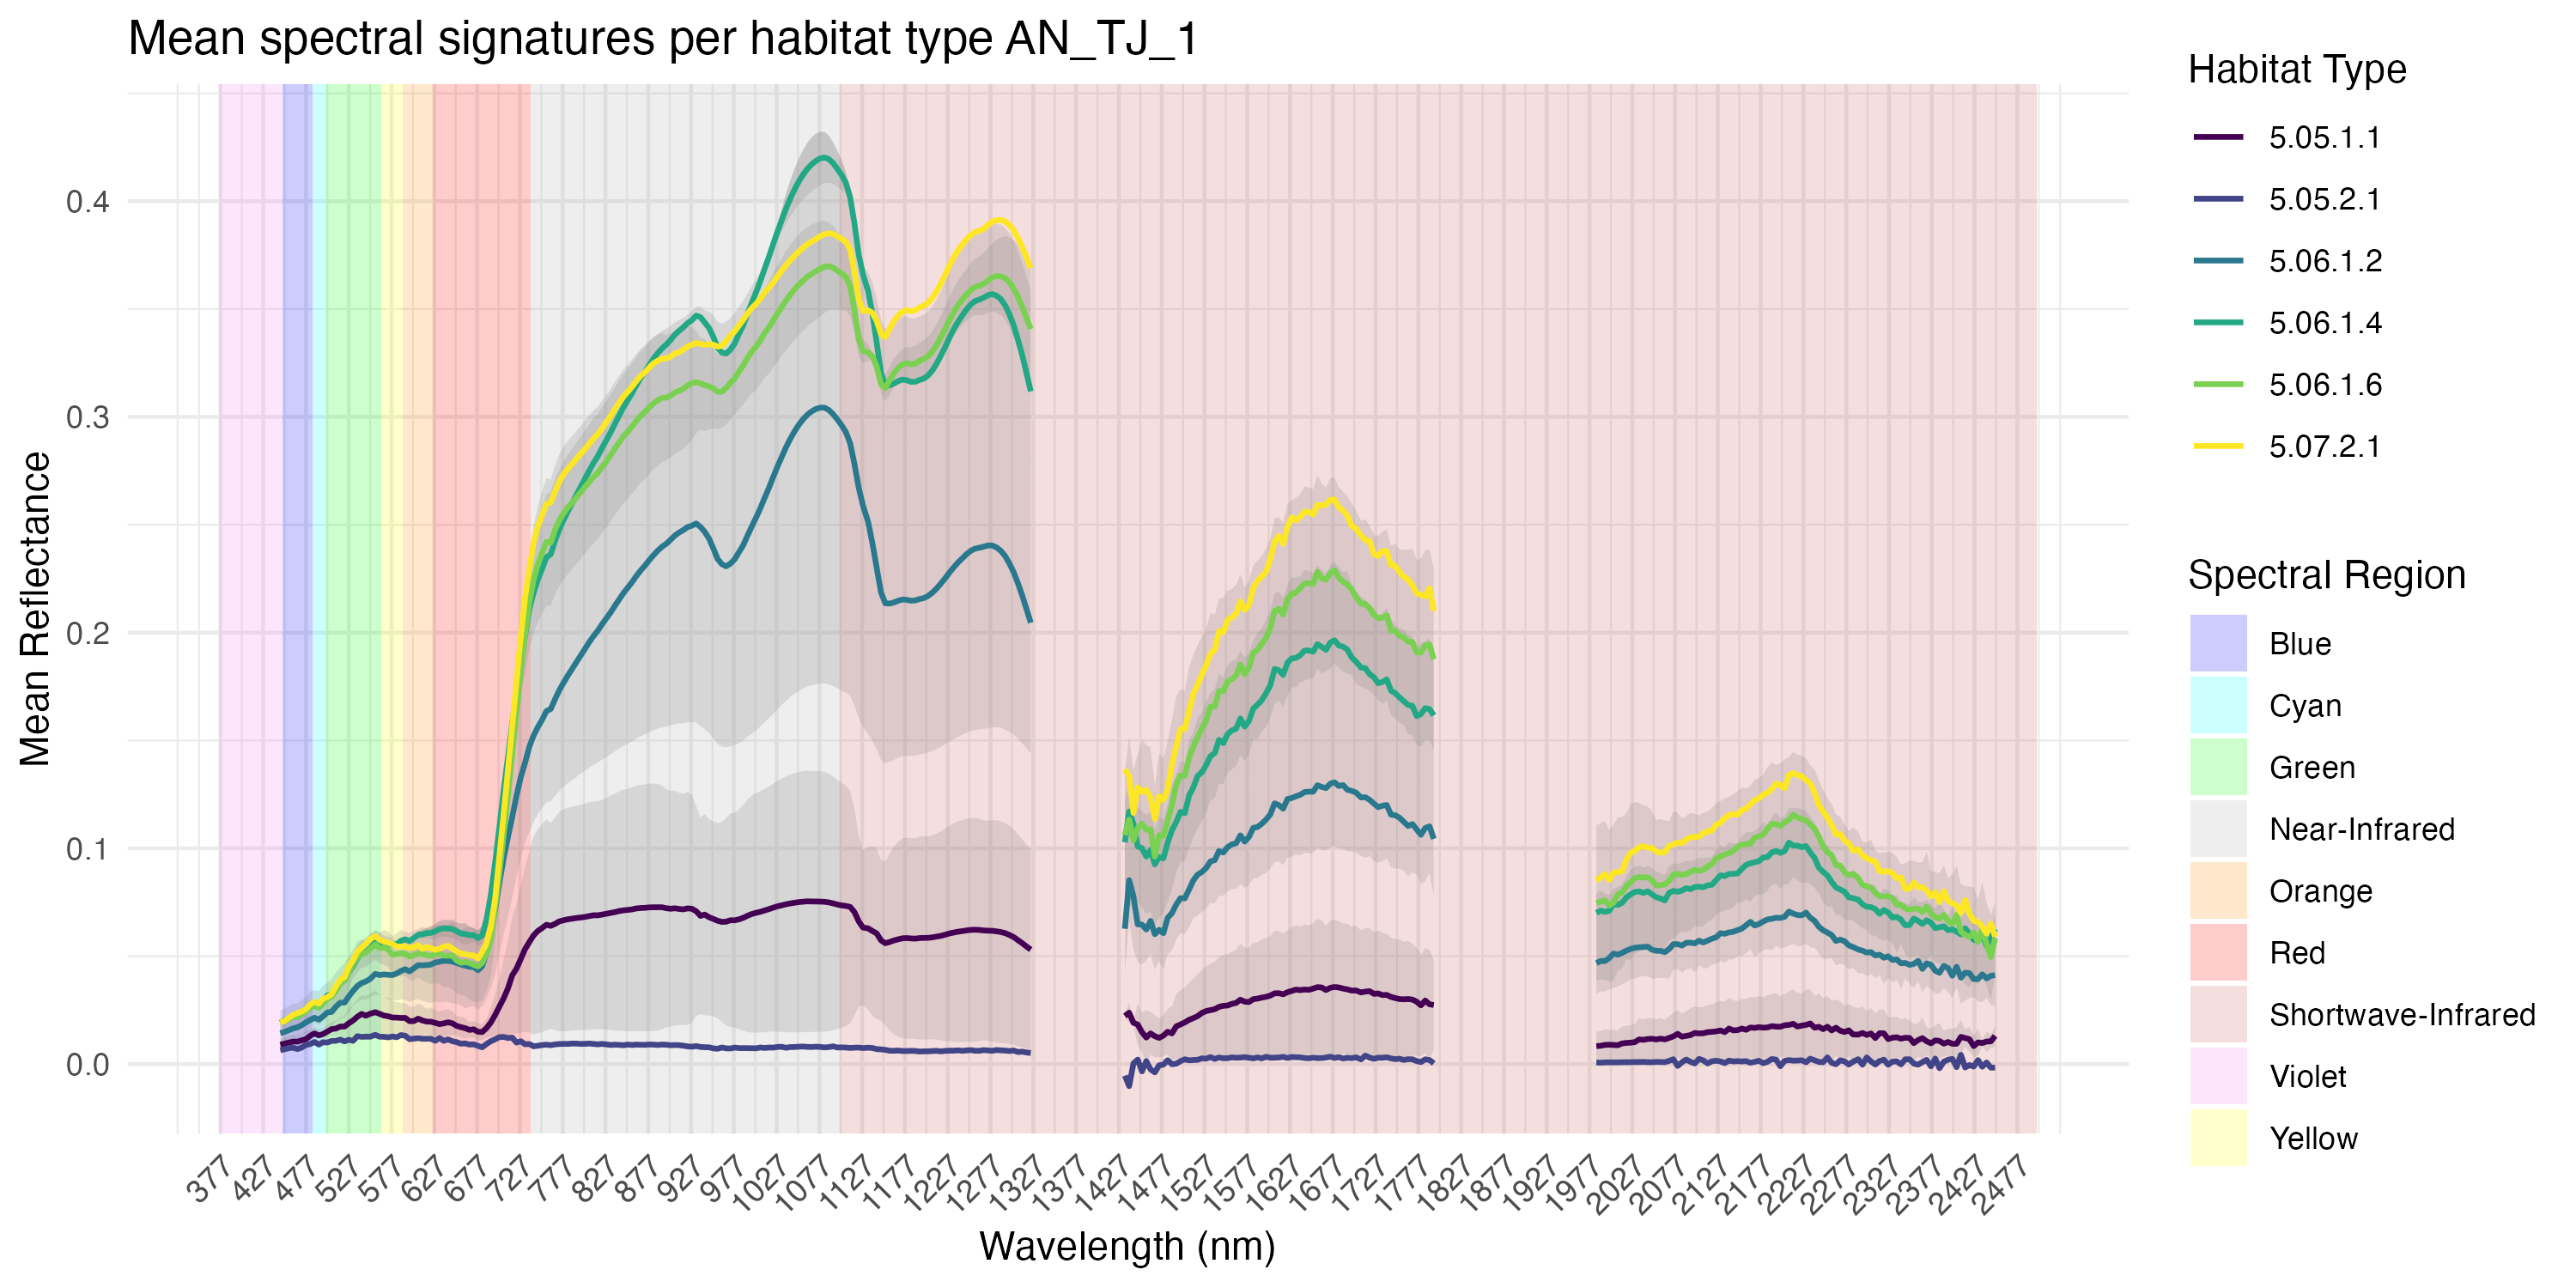
\includegraphics[width=\textwidth]{Figures/spectral_signatures/AN_TJ_1_mean_signature_plot_habitat.png}
    \caption{}
    \label{fig:mss_ht_antj1}
  \end{subfigure}

  \caption{Spectral signature plot \ref{fig:ss_ht_antj1} and mean spectral signature plot \ref{fig:mss_ht_antj1} grouped by habitat type for test site AN\_TJ\_1}
  \label{fig:group_ss_ht_antj1}
\end{figure}

\begin{figure}[H]
  \centering

  \begin{subfigure}[b]{0.49\textwidth}
    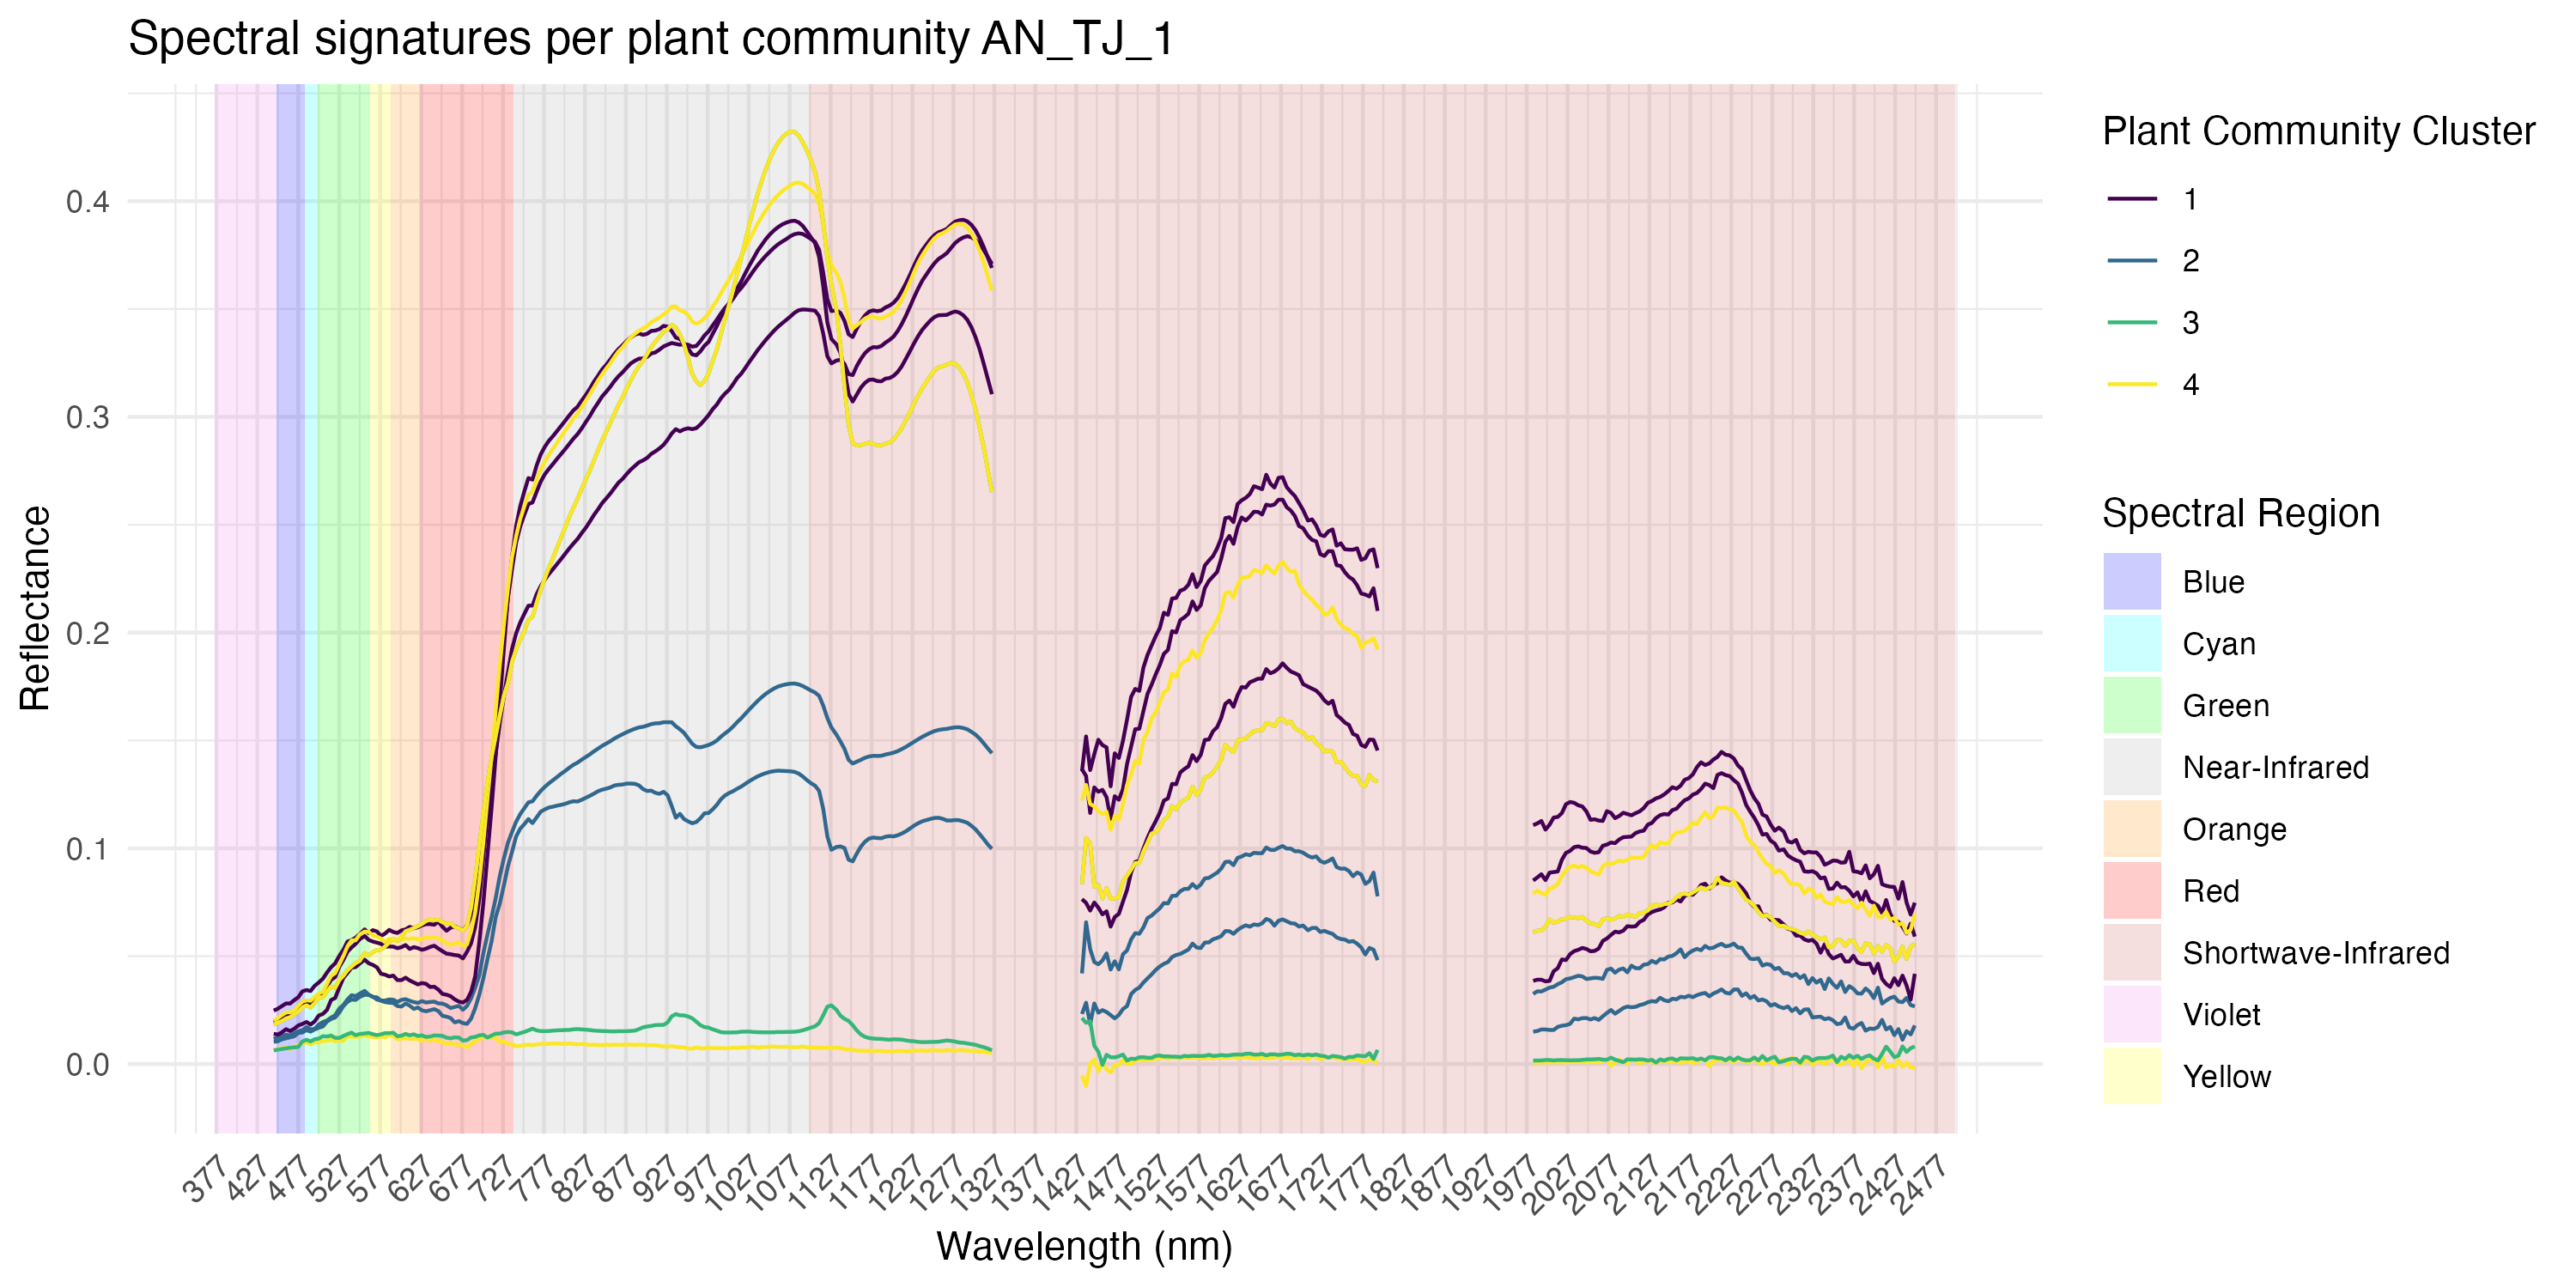
\includegraphics[width=\textwidth]{Figures/spectral_signatures/AN_TJ_1_signature_plot_plant_community.png}
    \caption{}
    \label{fig:ss_pc_antj1}
  \end{subfigure}
  \hfill
  \begin{subfigure}[b]{0.49\textwidth}
    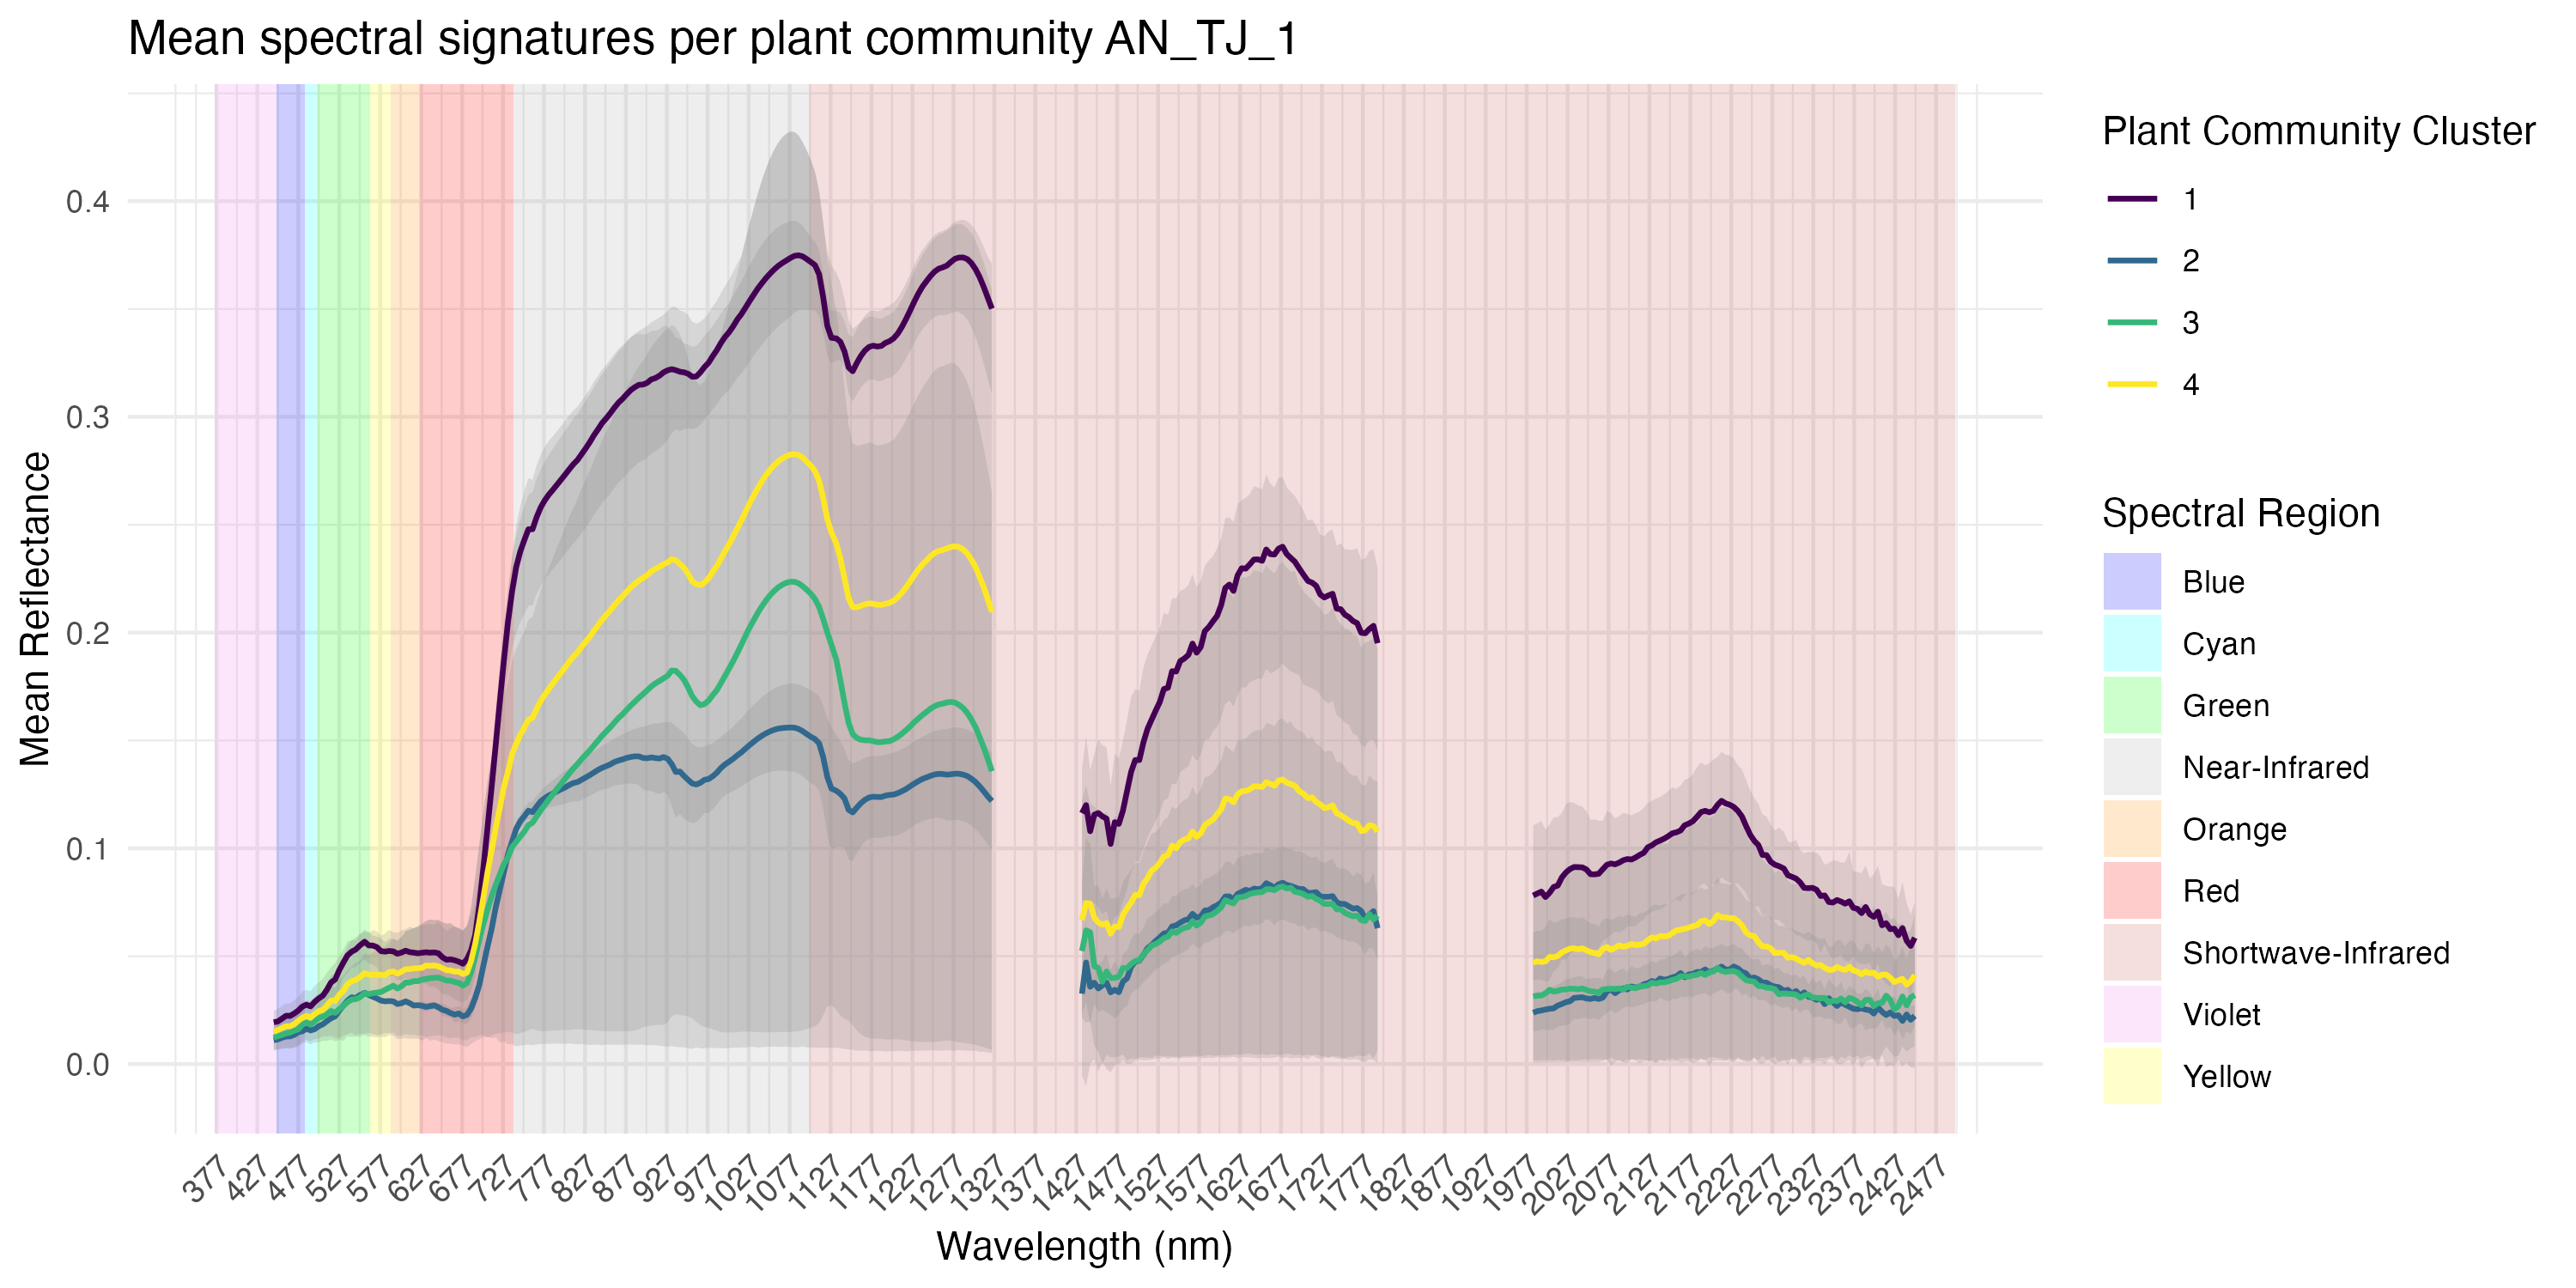
\includegraphics[width=\textwidth]{Figures/spectral_signatures/AN_TJ_1_mean_signature_plot_plant_community.png}
    \caption{}
    \label{fig:mss_pc_antj1}
  \end{subfigure}

  \caption{Spectral signature plot \ref{fig:ss_pc_antj1} and mean spectral signature plot \ref{fig:mss_pc_antj1} grouped by plant community cluster for test site AN\_TJ\_1}
  \label{fig:group_pc_ht_antj1}
\end{figure}

\subsection{AN\_TJ\_2}

\begin{figure}[H]
  \centering

  \begin{subfigure}[b]{0.49\textwidth}
    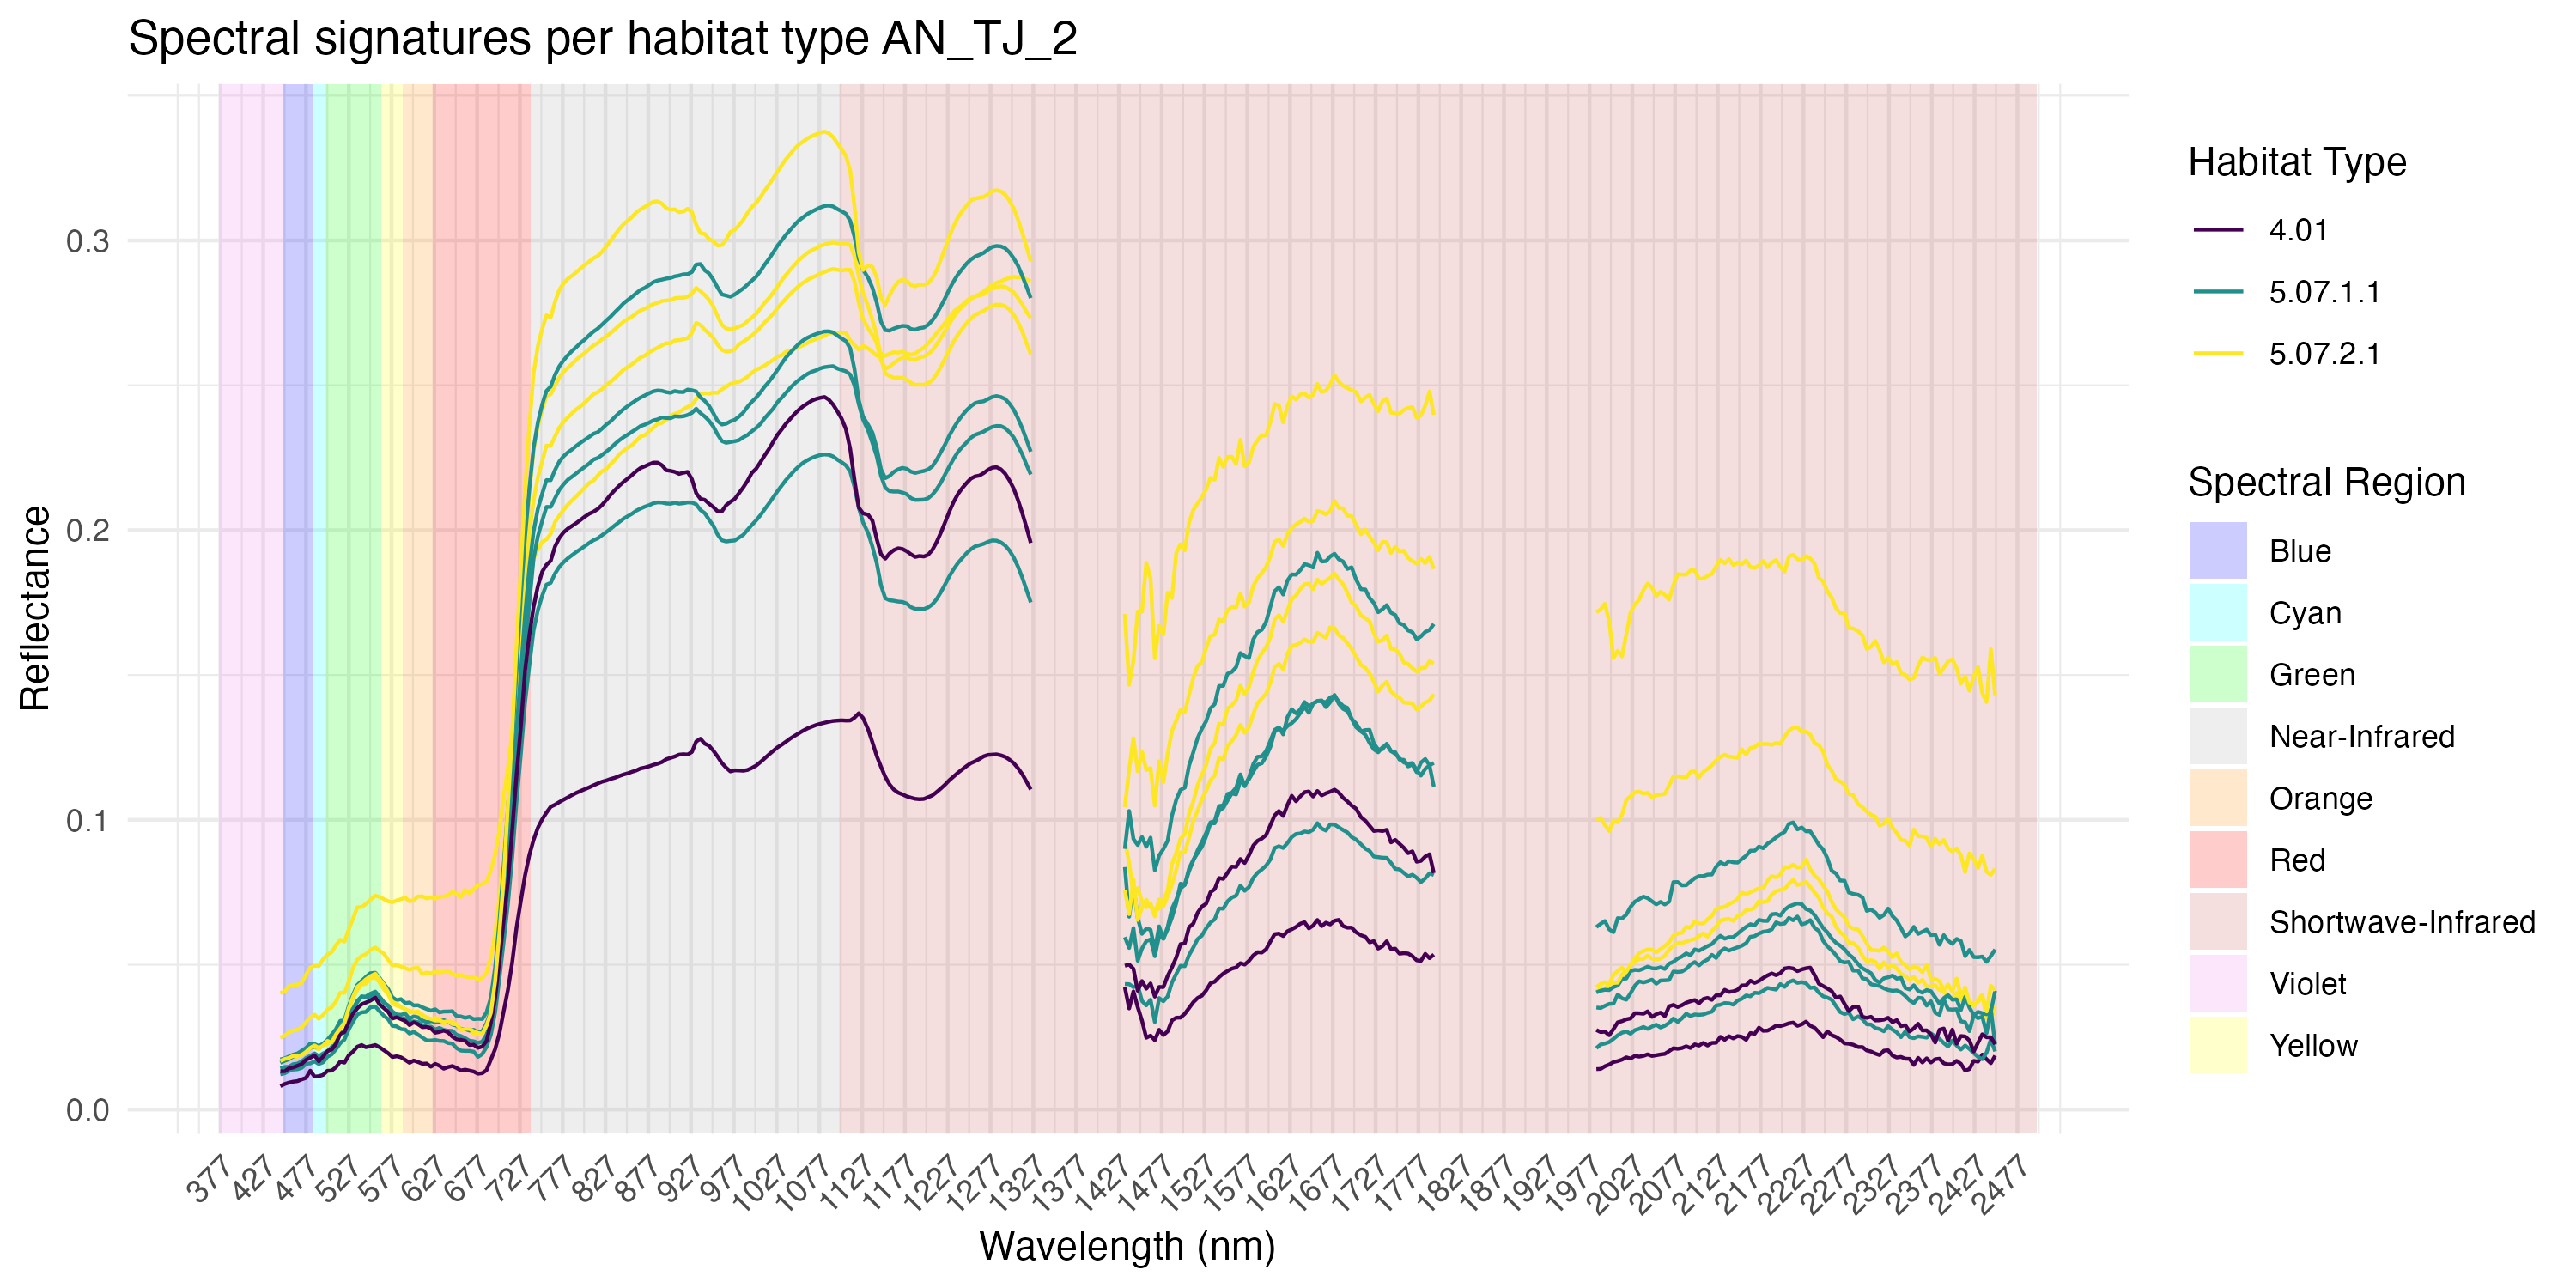
\includegraphics[width=\textwidth]{Figures/spectral_signatures/AN_TJ_2_signature_plot_habitat.png}
    \caption{}
    \label{fig:ss_ht_antj2}
  \end{subfigure}
  \hfill
  \begin{subfigure}[b]{0.49\textwidth}
    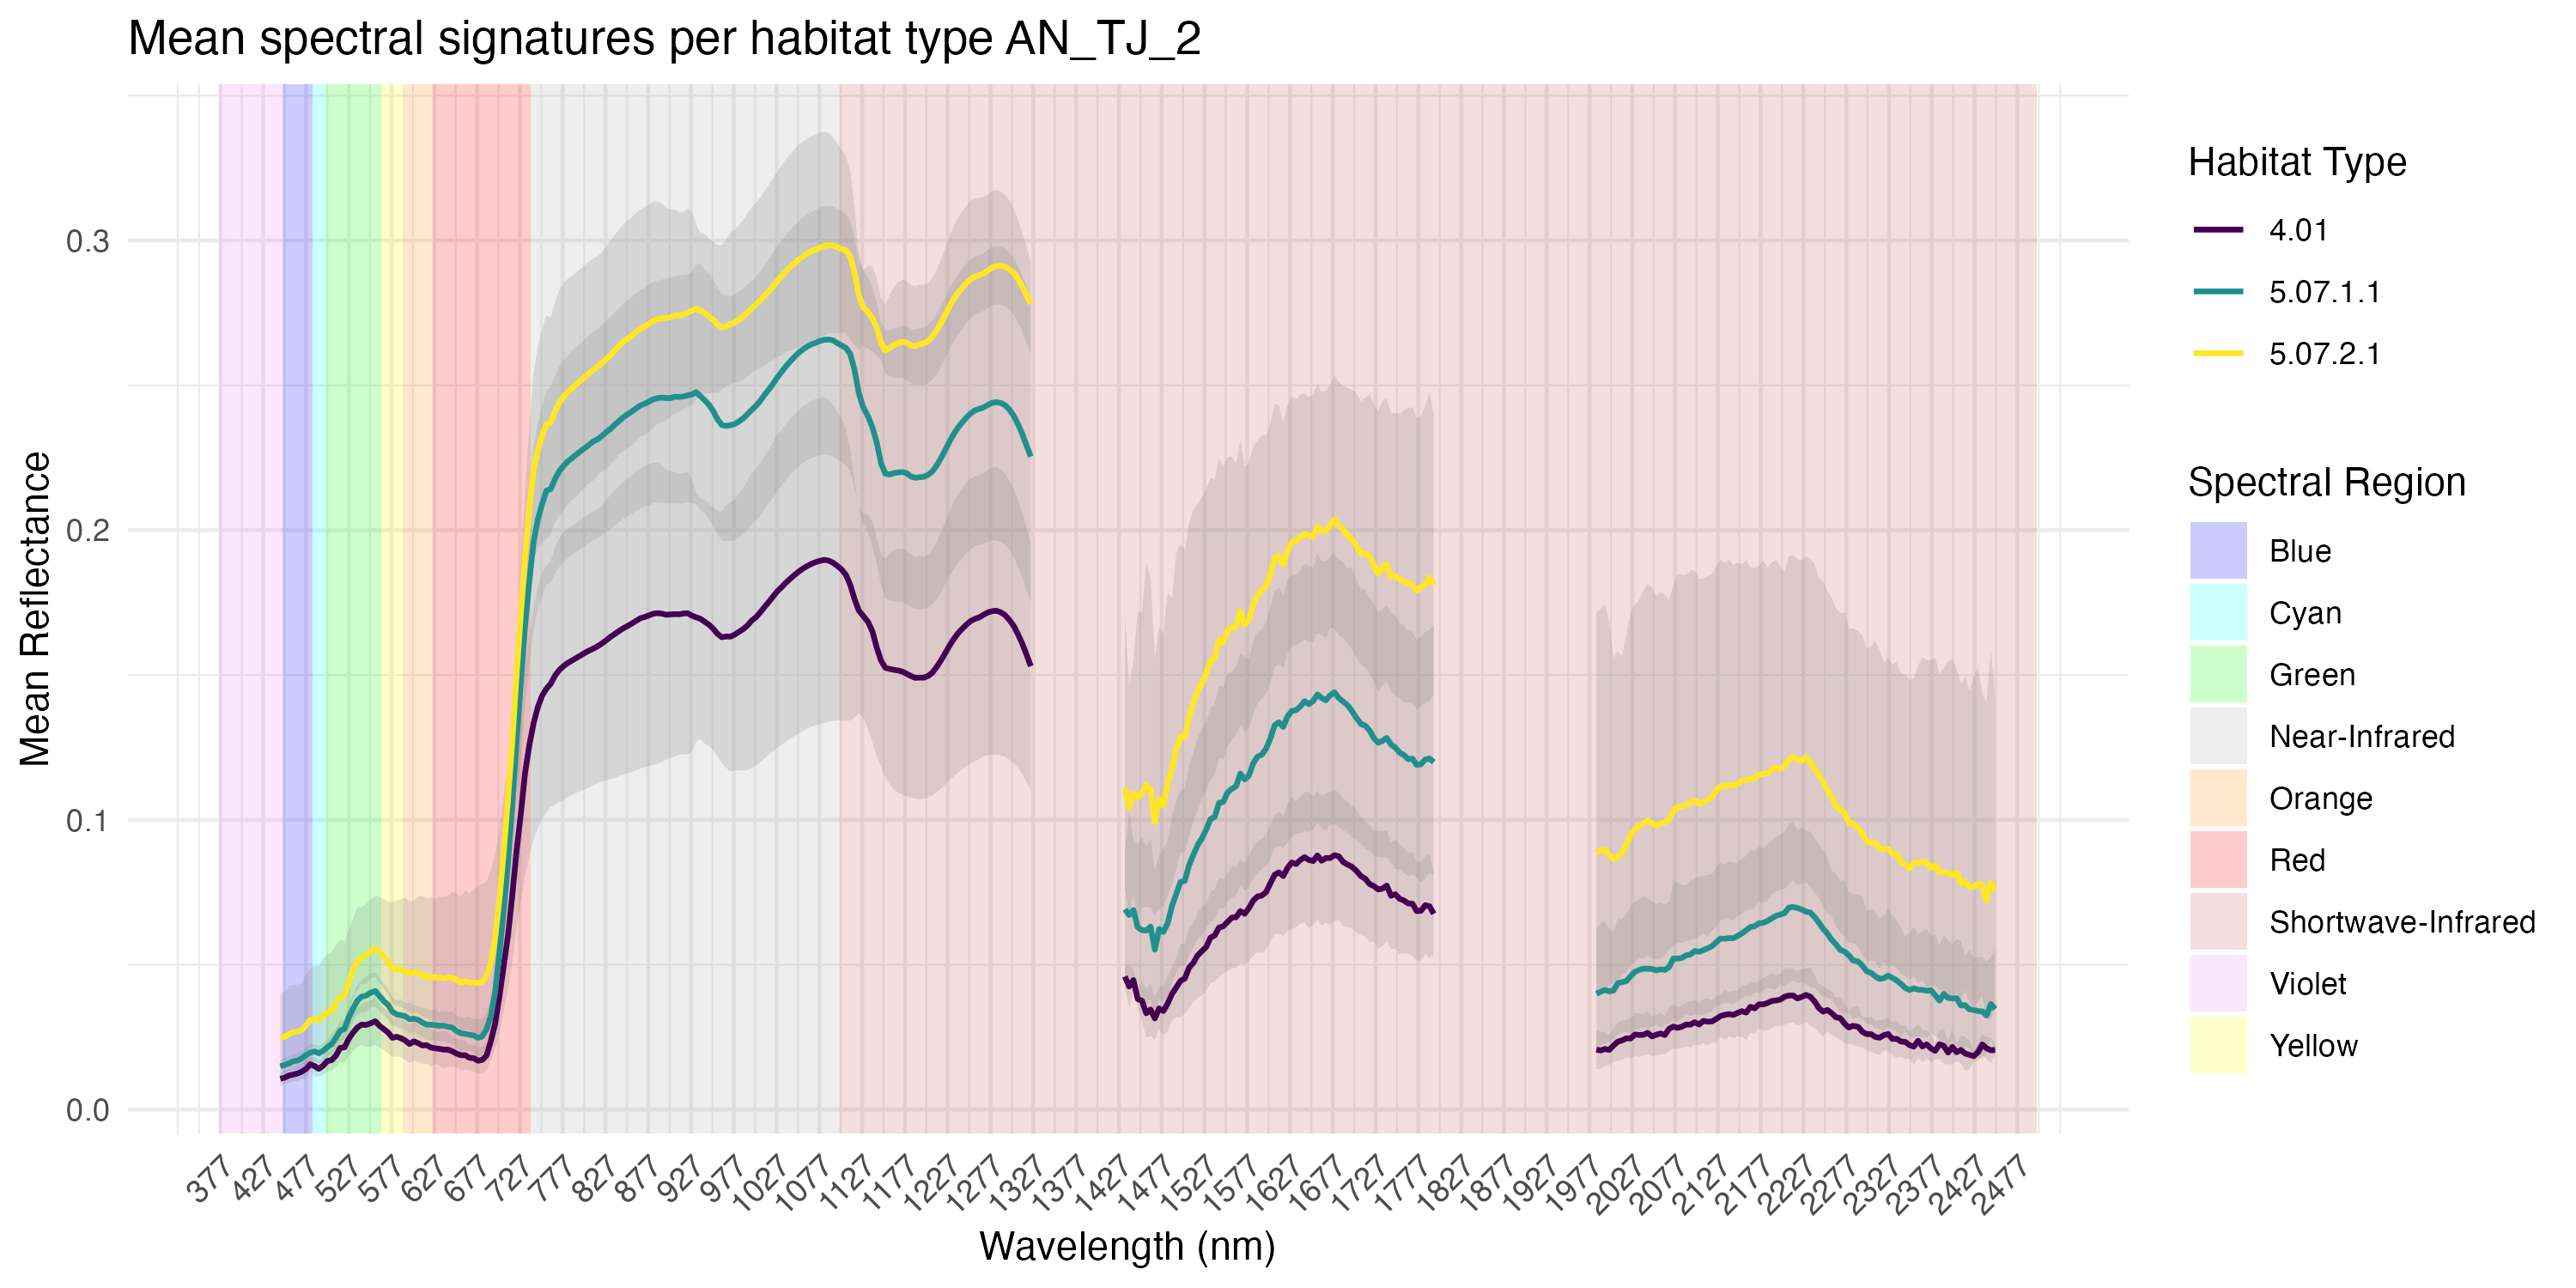
\includegraphics[width=\textwidth]{Figures/spectral_signatures/AN_TJ_2_mean_signature_plot_habitat.png}
    \caption{}
    \label{fig:mss_ht_antj2}
  \end{subfigure}

  \caption{Spectral signature plot \ref{fig:ss_ht_antj2} and mean spectral signature plot \ref{fig:mss_ht_antj2} grouped by habitat type for test site AN\_TJ\_2}
  \label{fig:group_ss_ht_antj2}
\end{figure}

\begin{figure}[H]
  \centering

  \begin{subfigure}[b]{0.49\textwidth}
    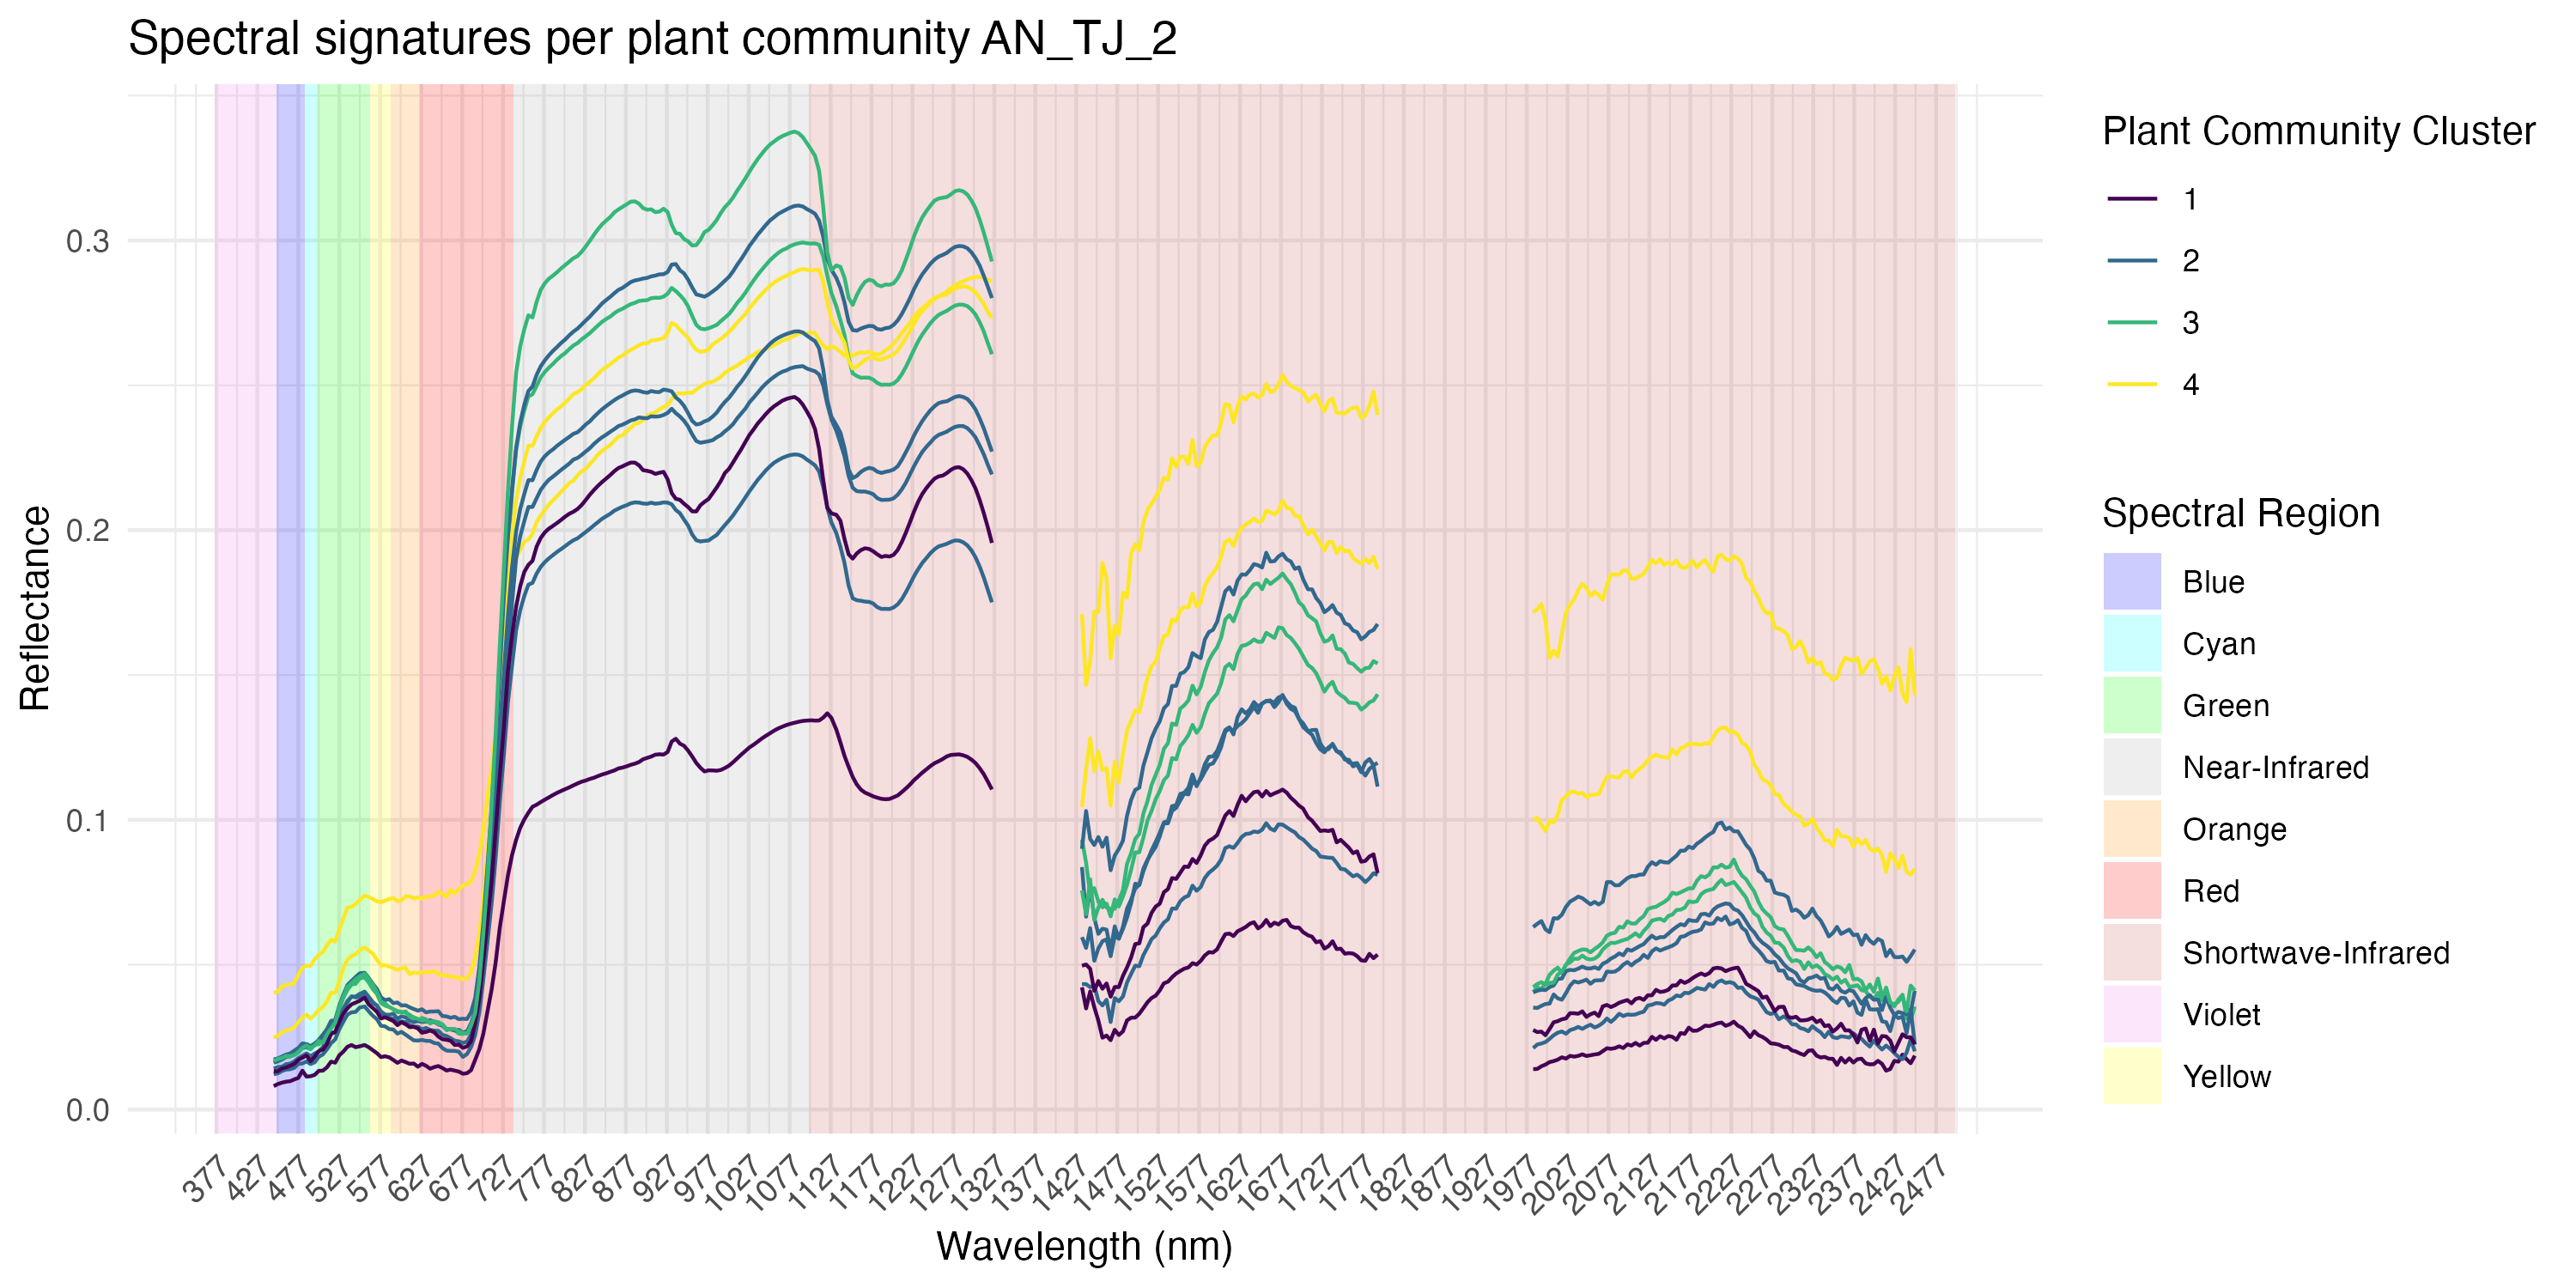
\includegraphics[width=\textwidth]{Figures/spectral_signatures/AN_TJ_2_signature_plot_plant_community.png}
    \caption{}
    \label{fig:ss_pc_antj2}
  \end{subfigure}
  \hfill
  \begin{subfigure}[b]{0.49\textwidth}
    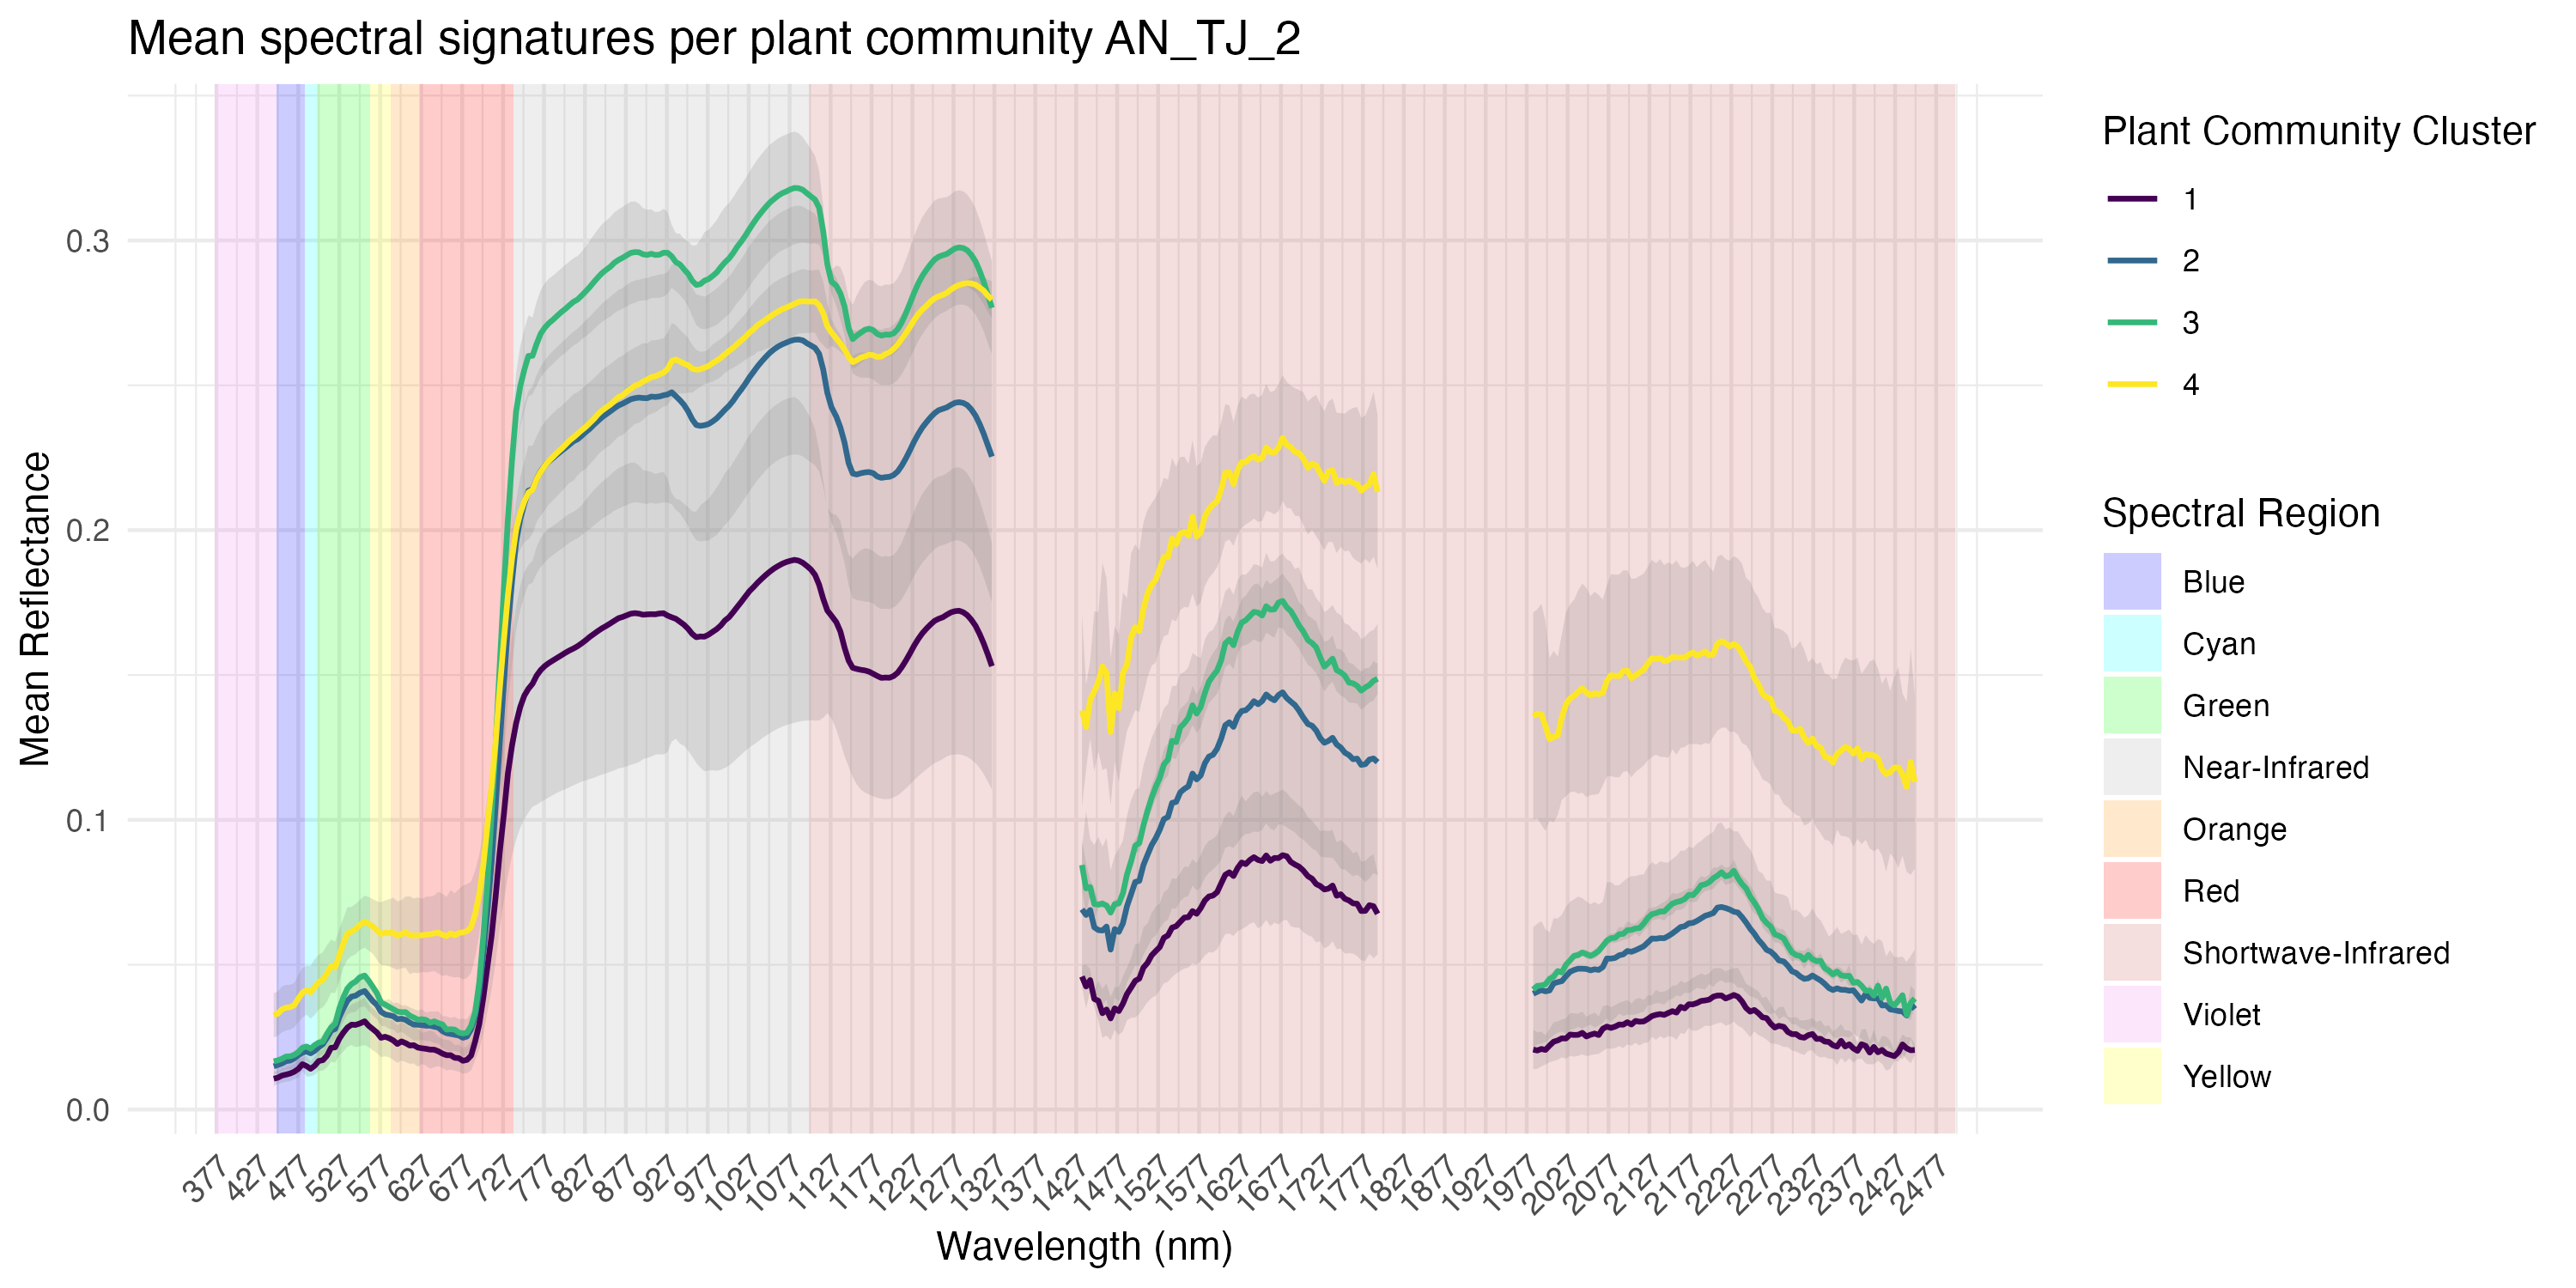
\includegraphics[width=\textwidth]{Figures/spectral_signatures/AN_TJ_2_mean_signature_plot_plant_community.png}
    \caption{}
    \label{fig:mss_pc_antj2}
  \end{subfigure}

  \caption{Spectral signature plot \ref{fig:ss_pc_antj2} and mean spectral signature plot \ref{fig:mss_pc_antj2} grouped by plant community cluster for test site AN\_TJ\_2}
  \label{fig:group_pc_ht_antj2}
\end{figure}

\subsection{ATQ\_VK\_1}

\begin{figure}[H]
  \centering

  \begin{subfigure}[b]{0.49\textwidth}
    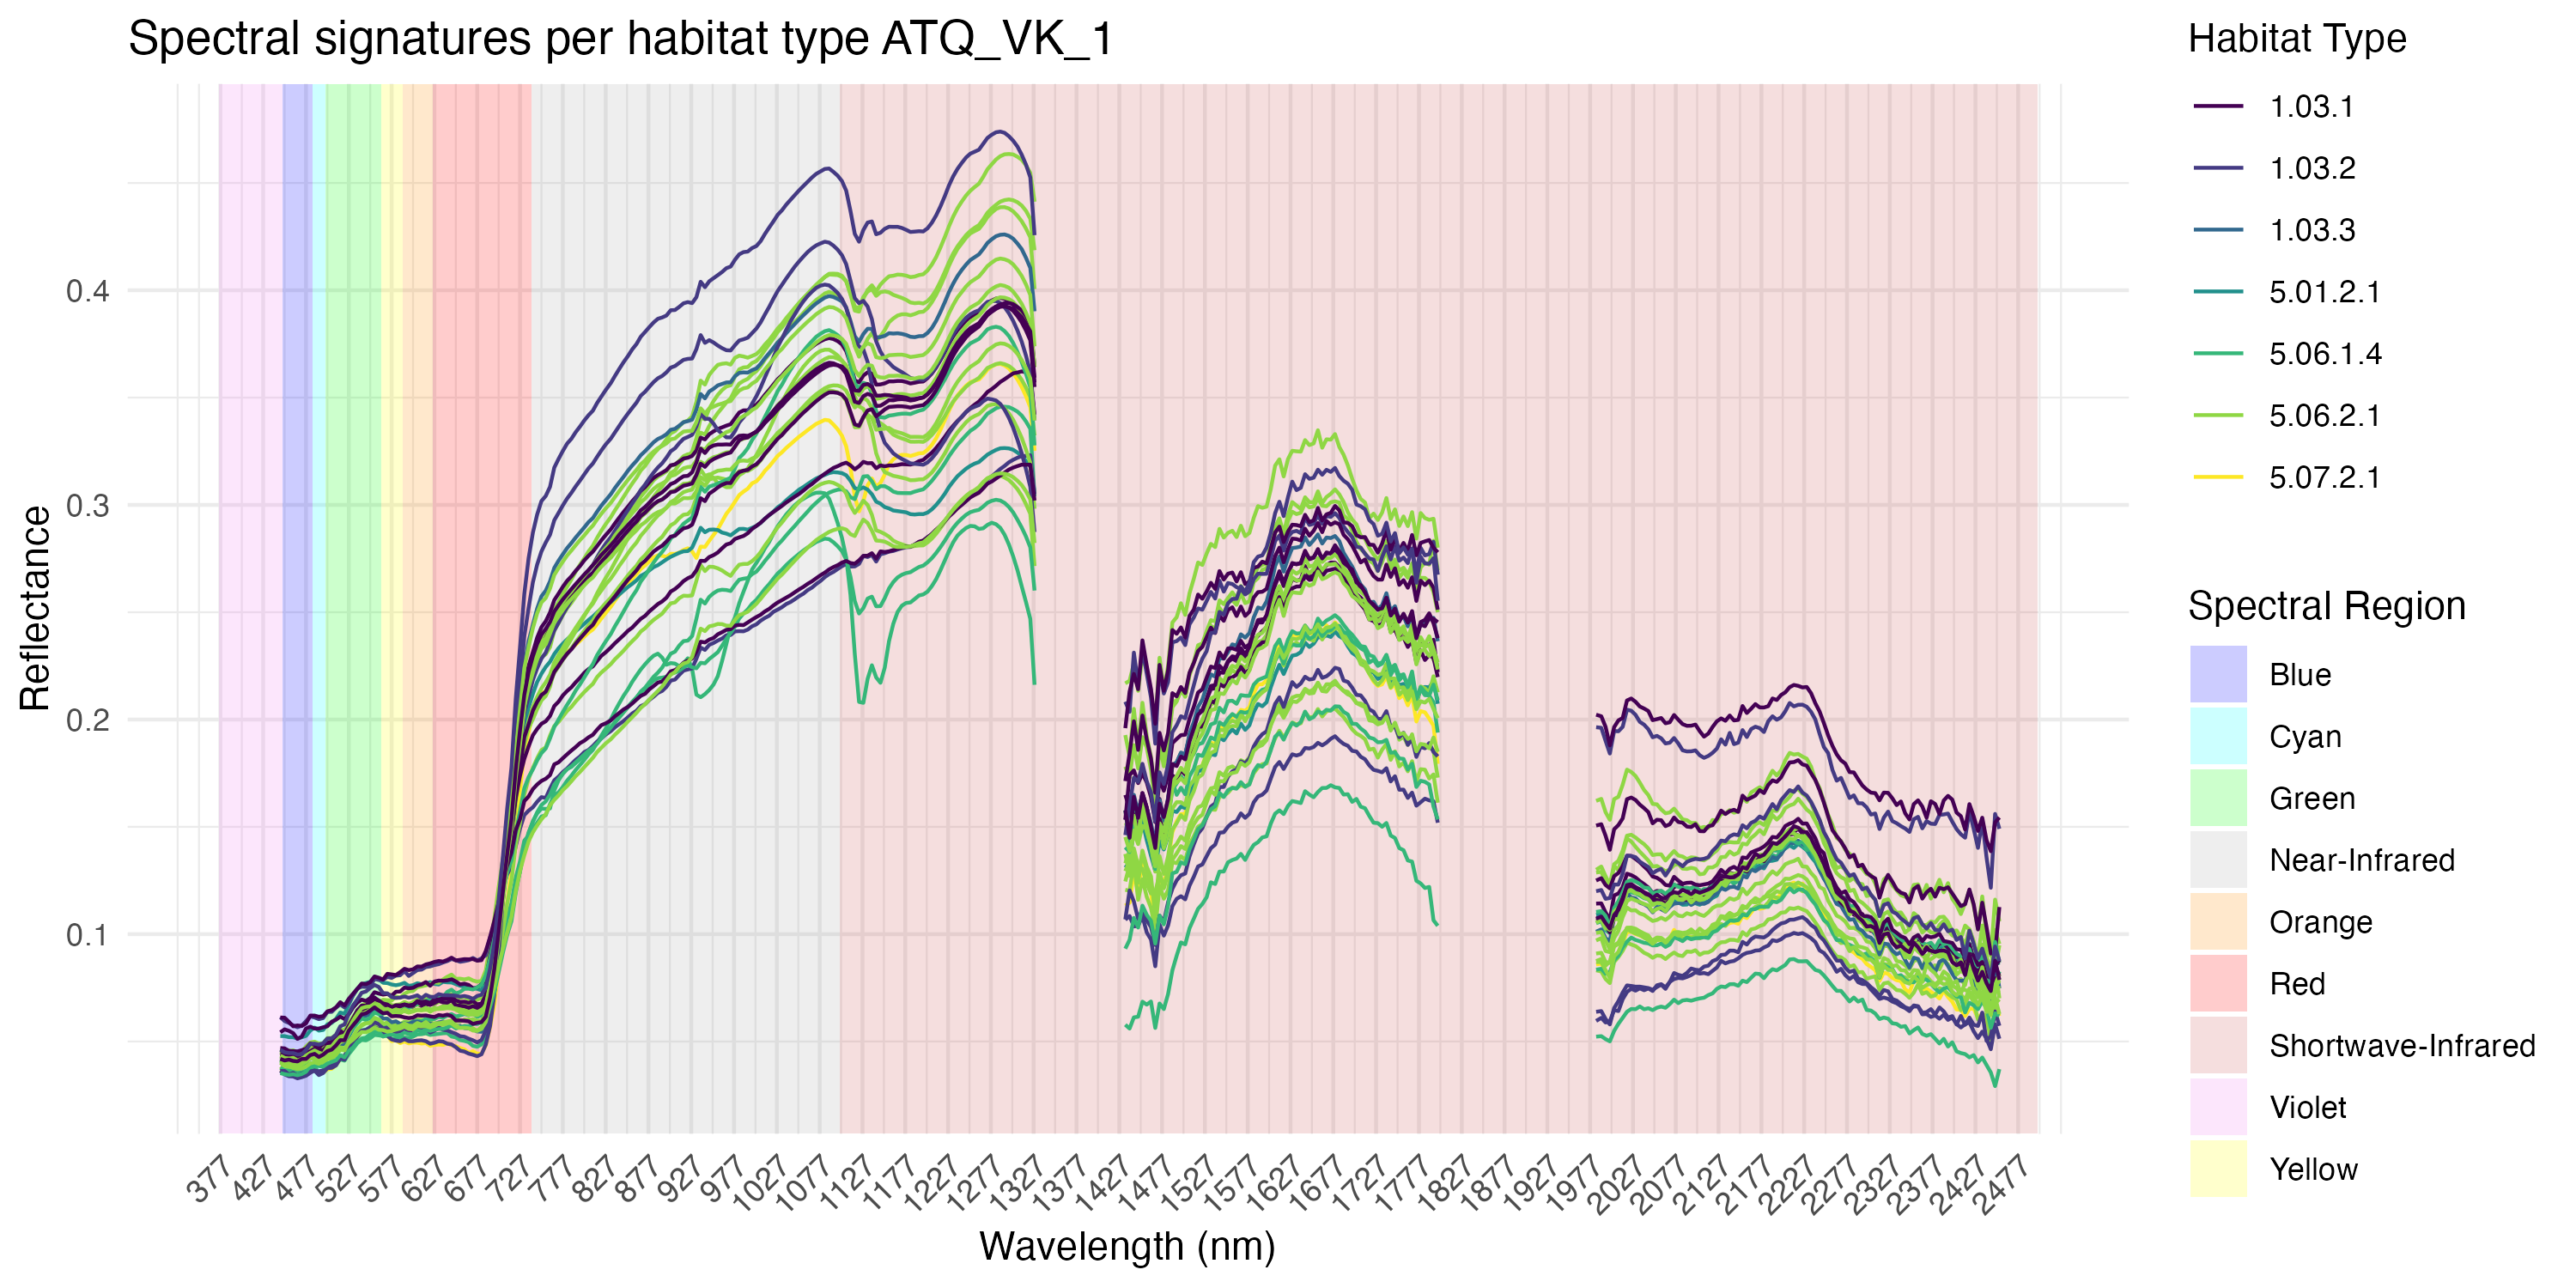
\includegraphics[width=\textwidth]{Figures/spectral_signatures/ATQ_VK_1_signature_plot_habitat.png}
    \caption{}
    \label{fig:ss_ht_atqvk1}
  \end{subfigure}
  \hfill
  \begin{subfigure}[b]{0.49\textwidth}
    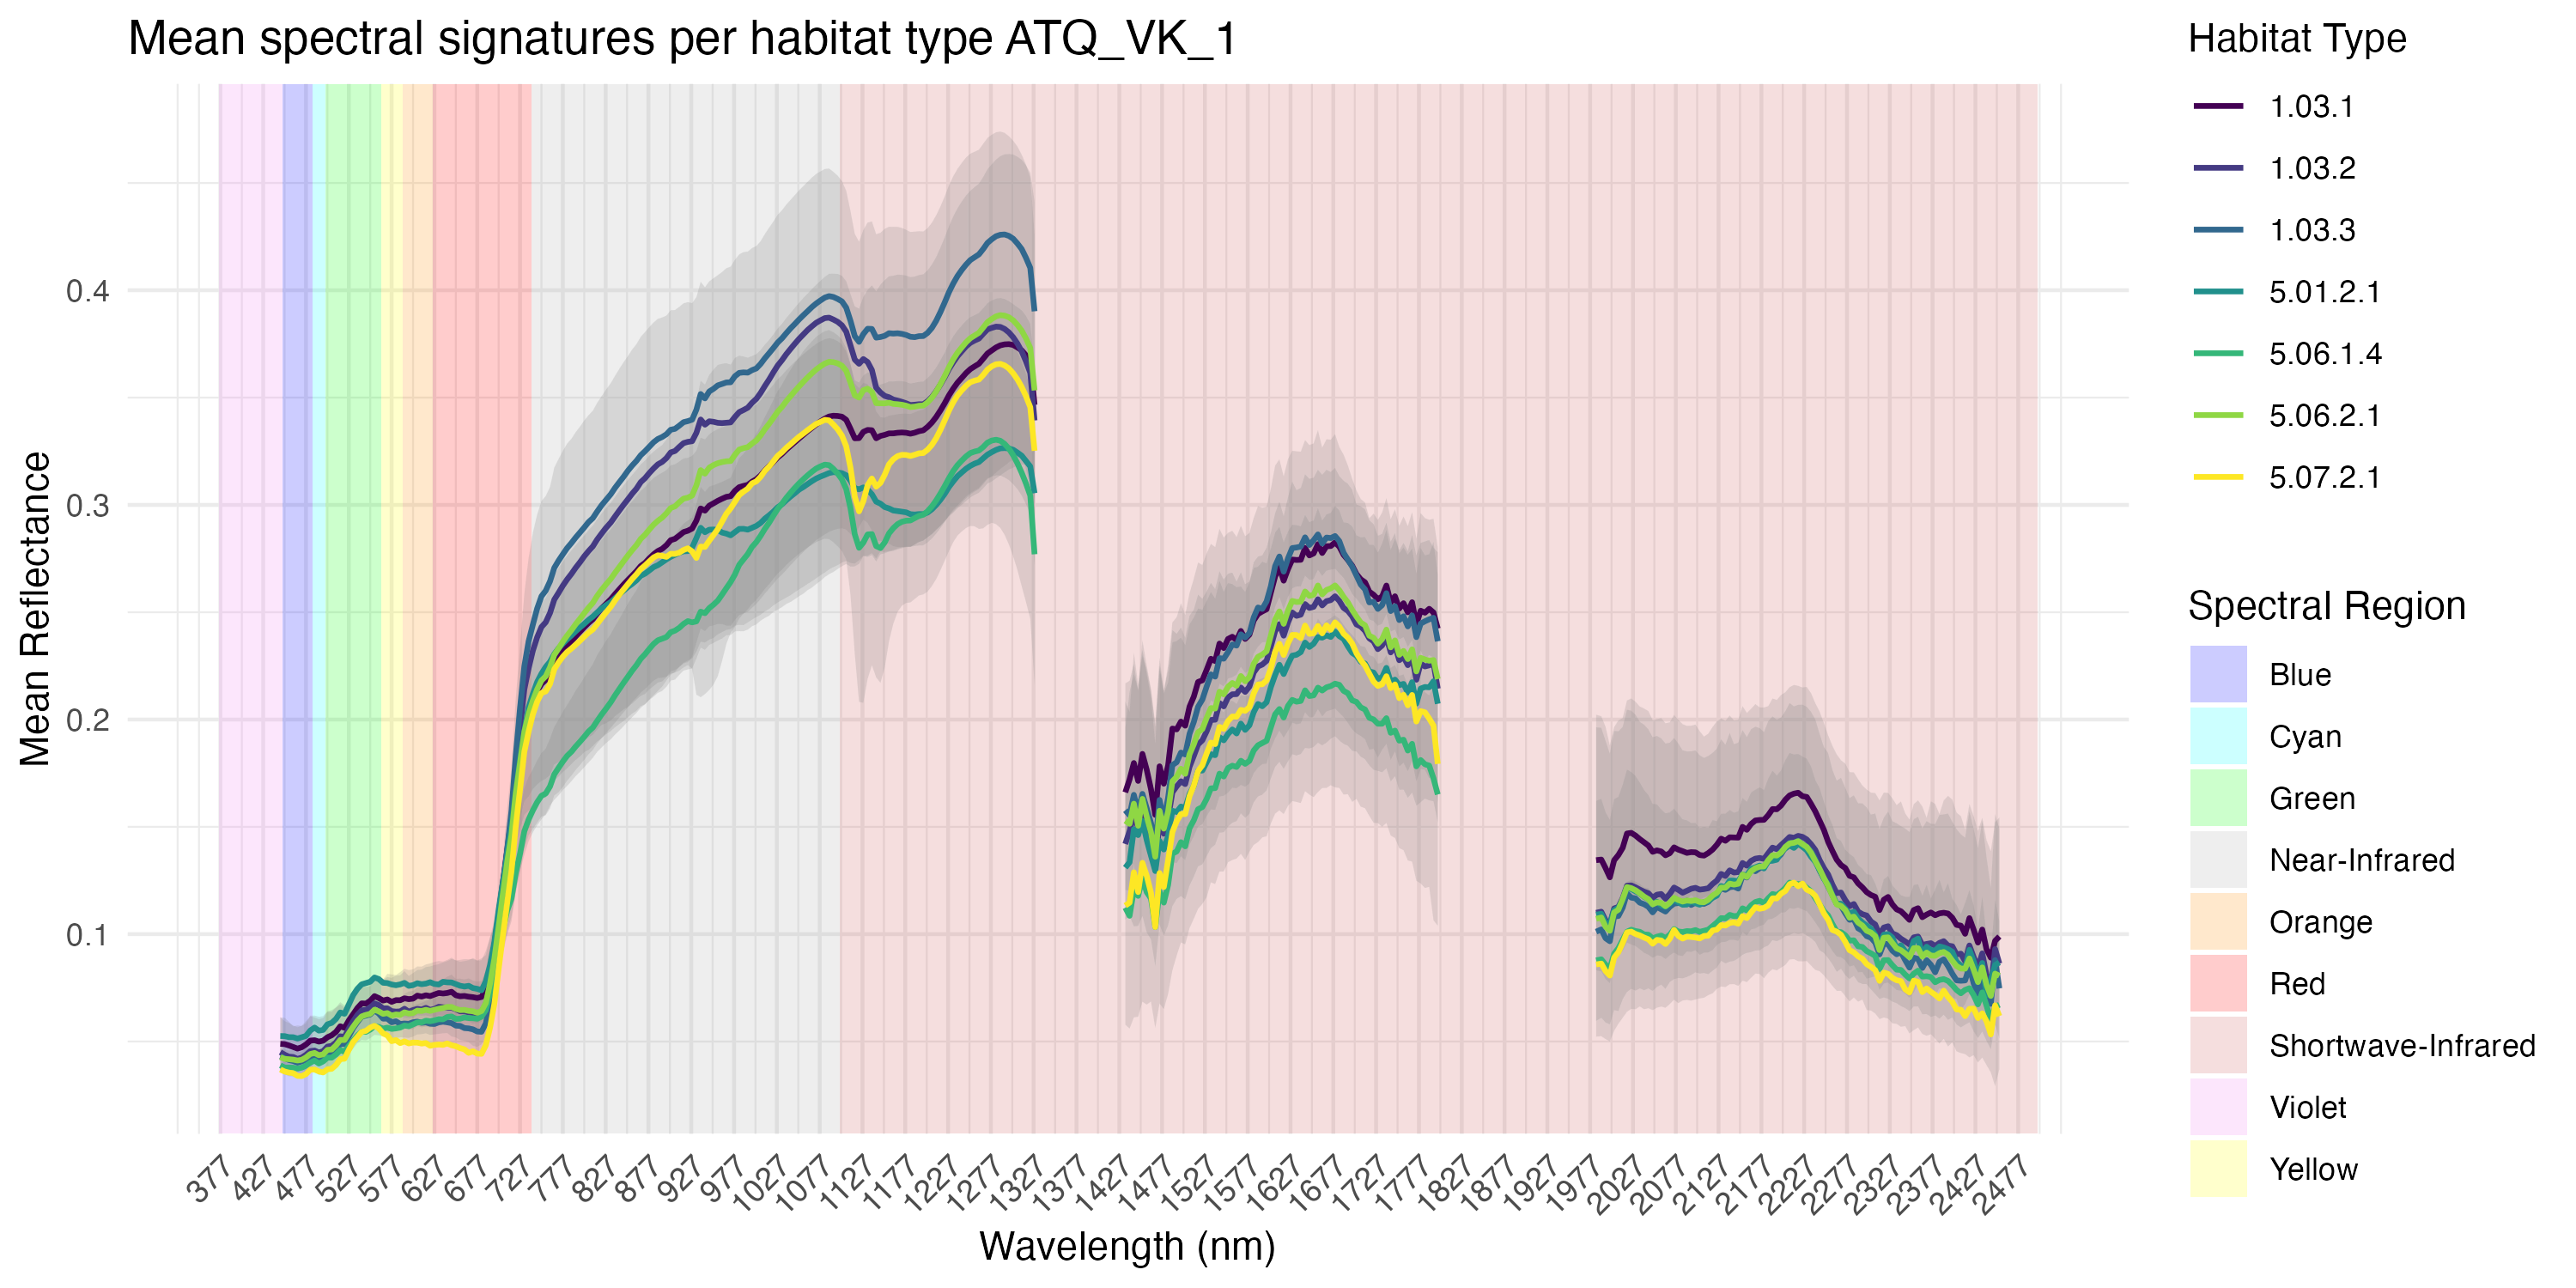
\includegraphics[width=\textwidth]{Figures/spectral_signatures/ATQ_VK_1_mean_signature_plot_habitat.png}
    \caption{}
    \label{fig:mss_ht_atqvk1}
  \end{subfigure}

  \caption{Spectral signature plot \ref{fig:ss_ht_atqvk1} and mean spectral signature plot \ref{fig:mss_ht_atqvk1} grouped by habitat type for test site ATQ\_VK\_1}
  \label{fig:group_ss_ht_atqvk1}
\end{figure}

\begin{figure}[H]
  \centering

  \begin{subfigure}[b]{0.49\textwidth}
    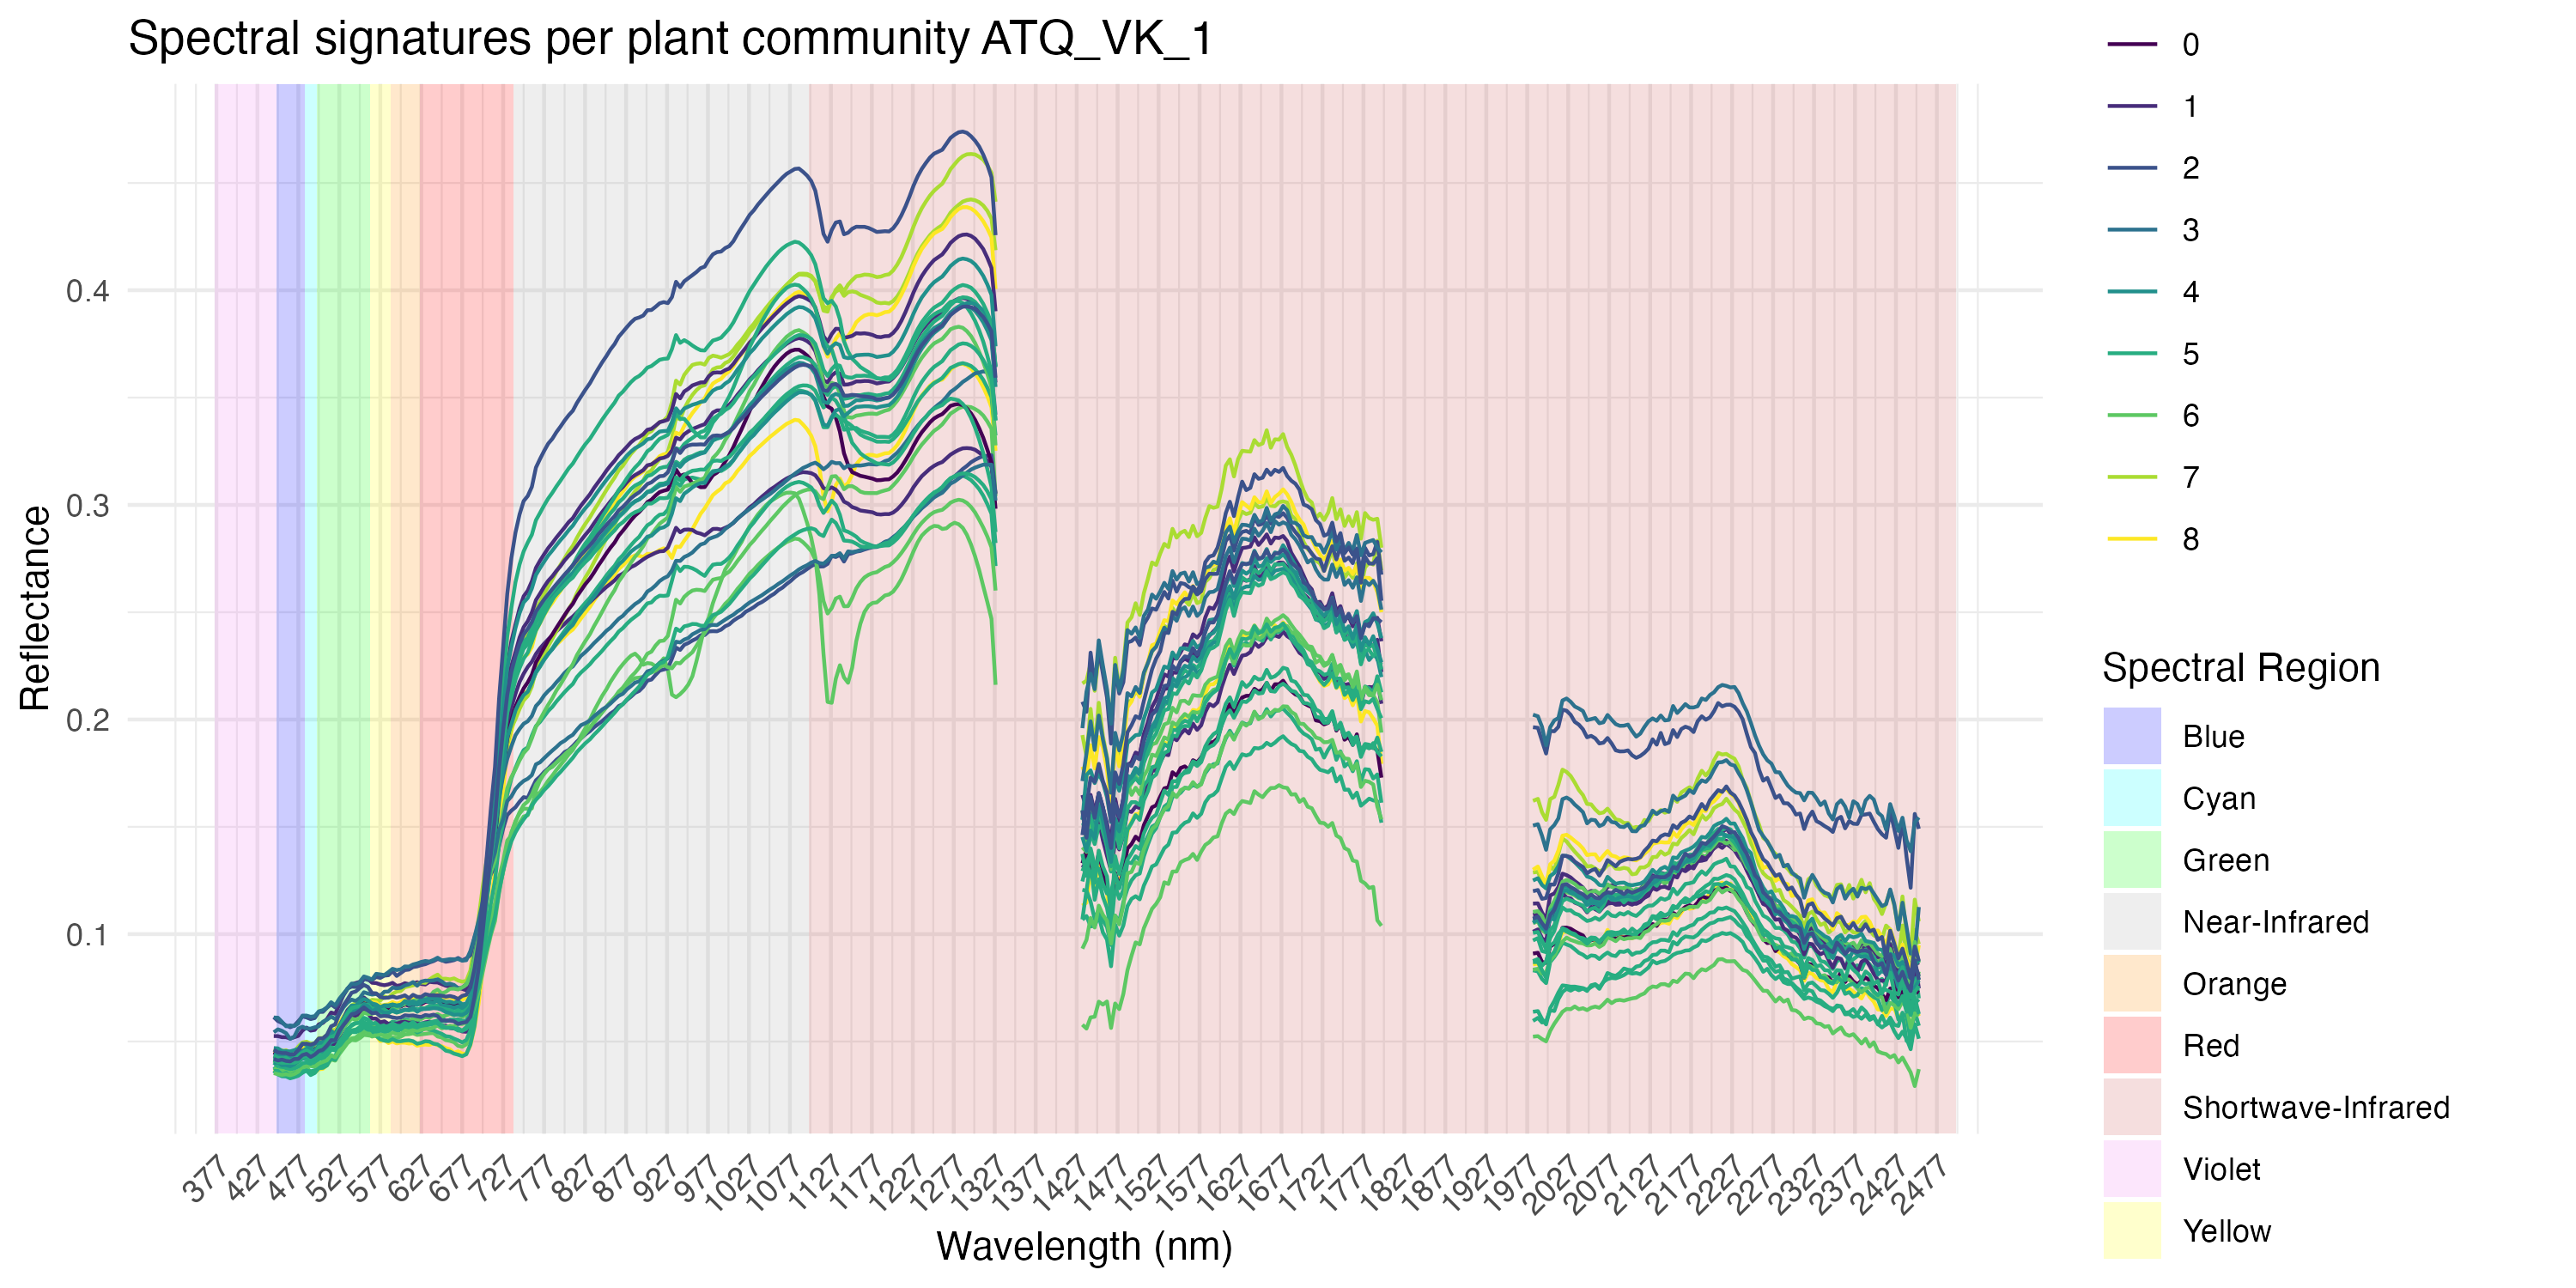
\includegraphics[width=\textwidth]{Figures/spectral_signatures/ATQ_VK_1_signature_plot_plant_community.png}
    \caption{}
    \label{fig:ss_pc_atqvk1}
  \end{subfigure}
  \hfill
  \begin{subfigure}[b]{0.49\textwidth}
    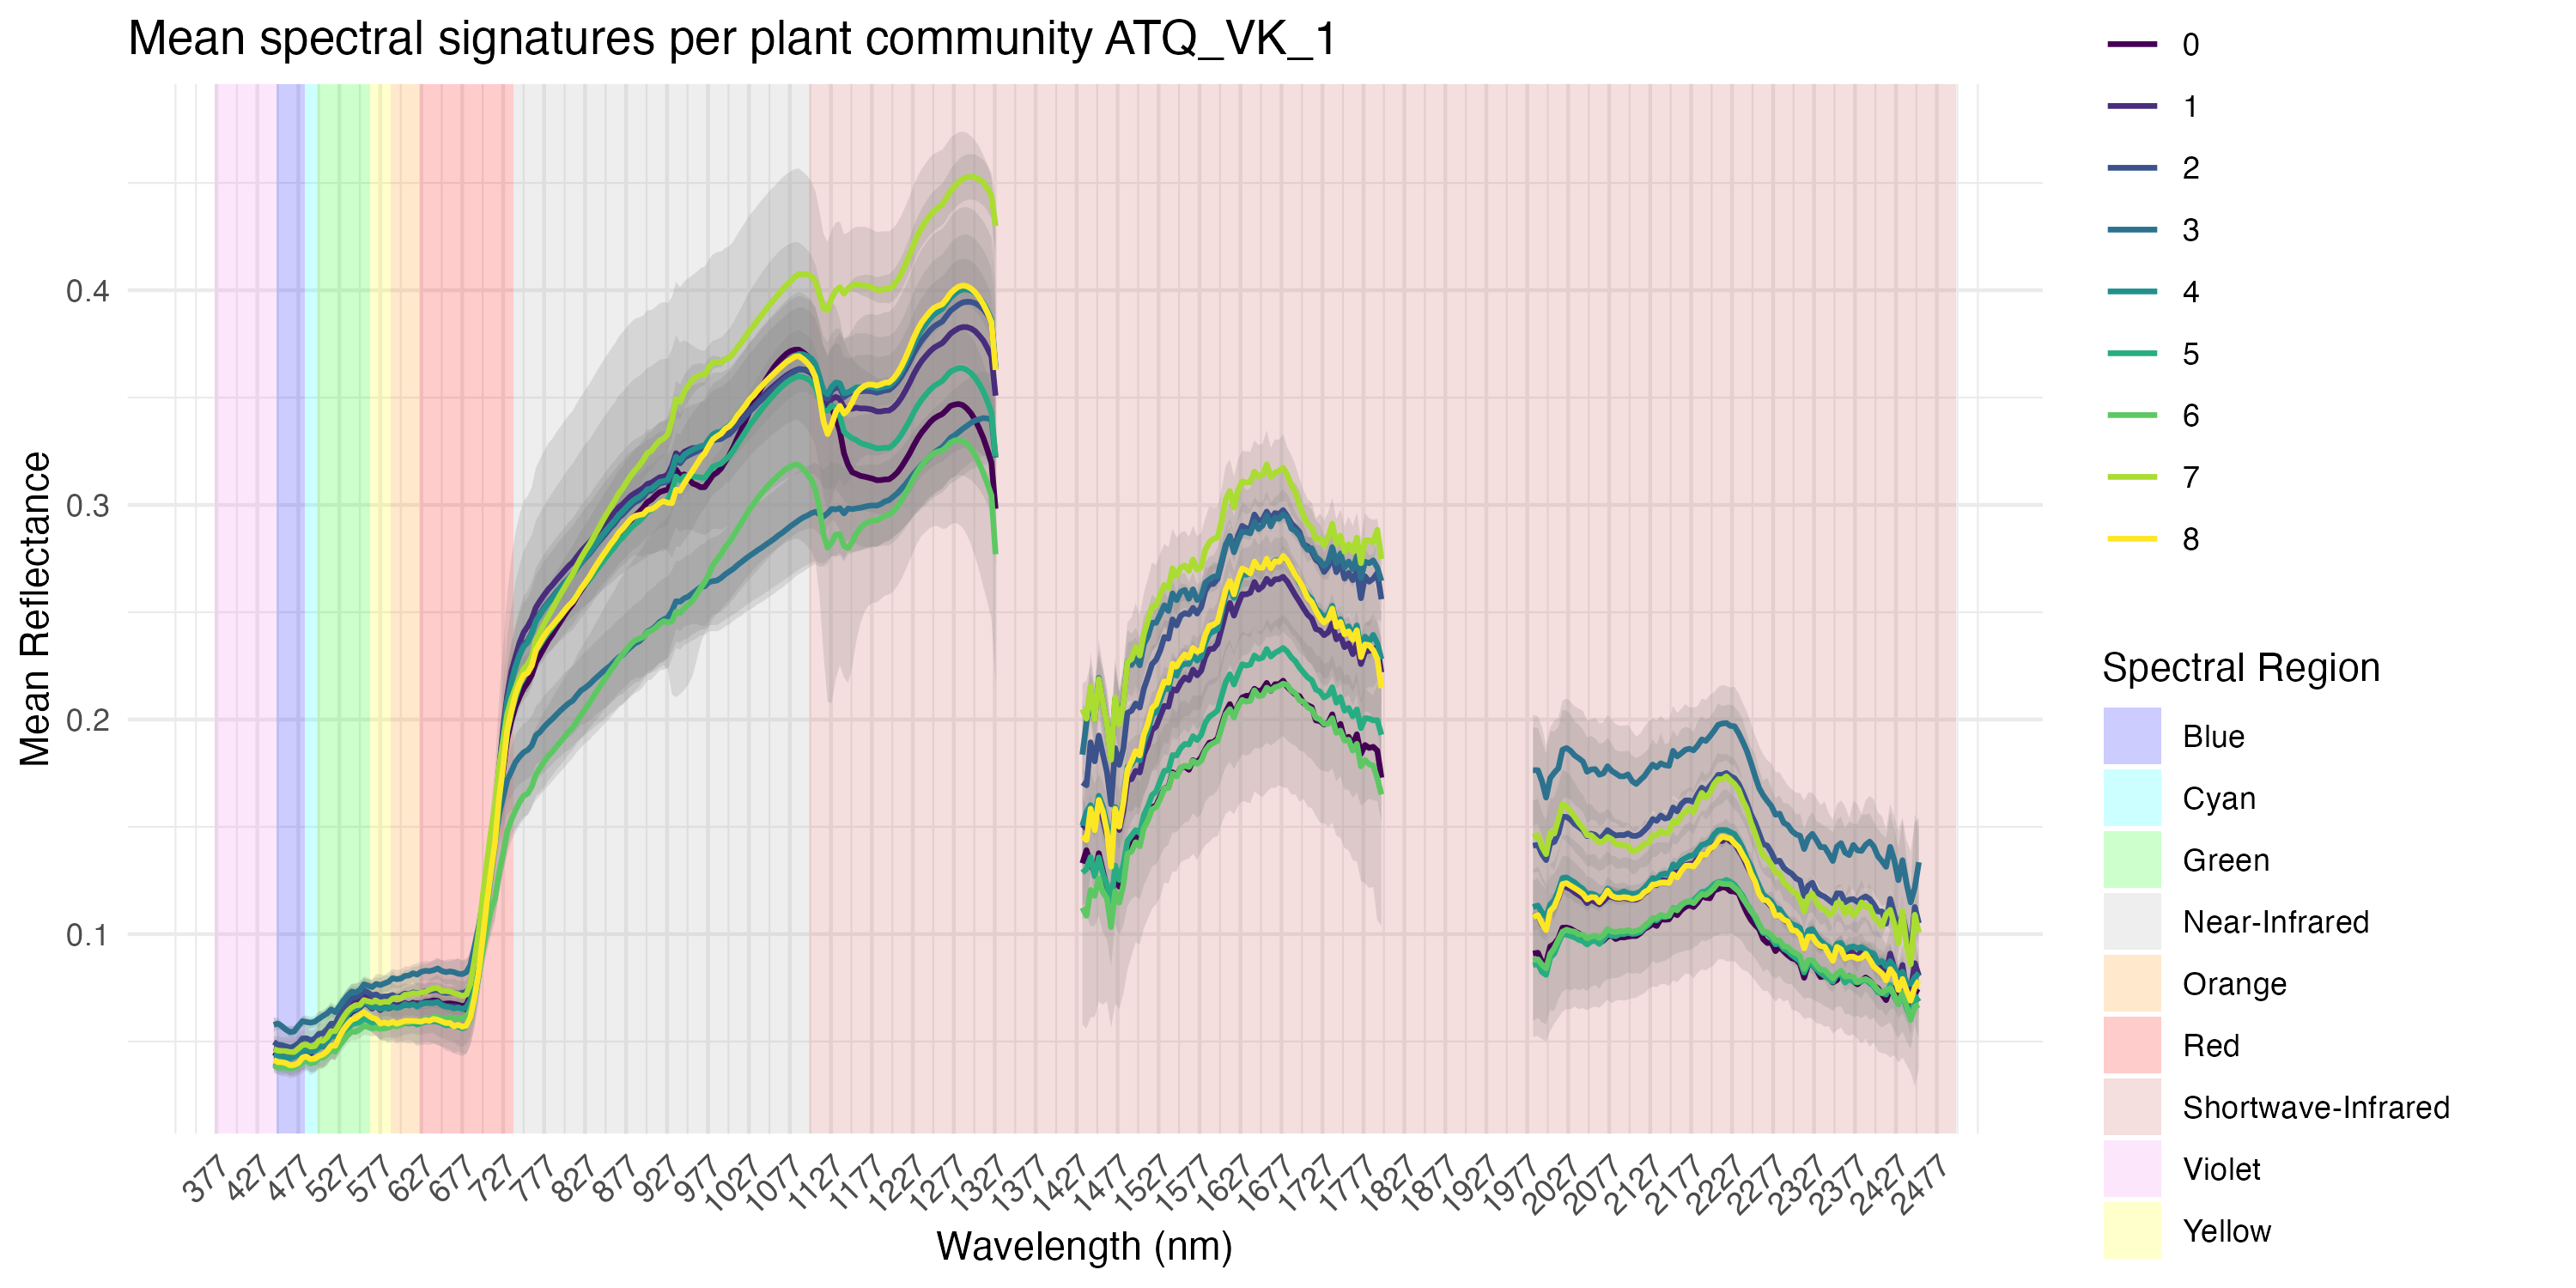
\includegraphics[width=\textwidth]{Figures/spectral_signatures/ATQ_VK_1_mean_signature_plot_plant_community.png}
    \caption{}
    \label{fig:mss_pc_atqvk1}
  \end{subfigure}

  \caption{Spectral signature plot \ref{fig:ss_pc_atqvk1} and mean spectral signature plot \ref{fig:mss_pc_atqvk1} grouped by plant community cluster for test site ATQ\_VK\_1}
  \label{fig:group_pc_ht_atqvk1}
\end{figure}

\subsection{BRW\_PW\_1}

\begin{figure}[H]
  \centering

  \begin{subfigure}[b]{0.49\textwidth}
    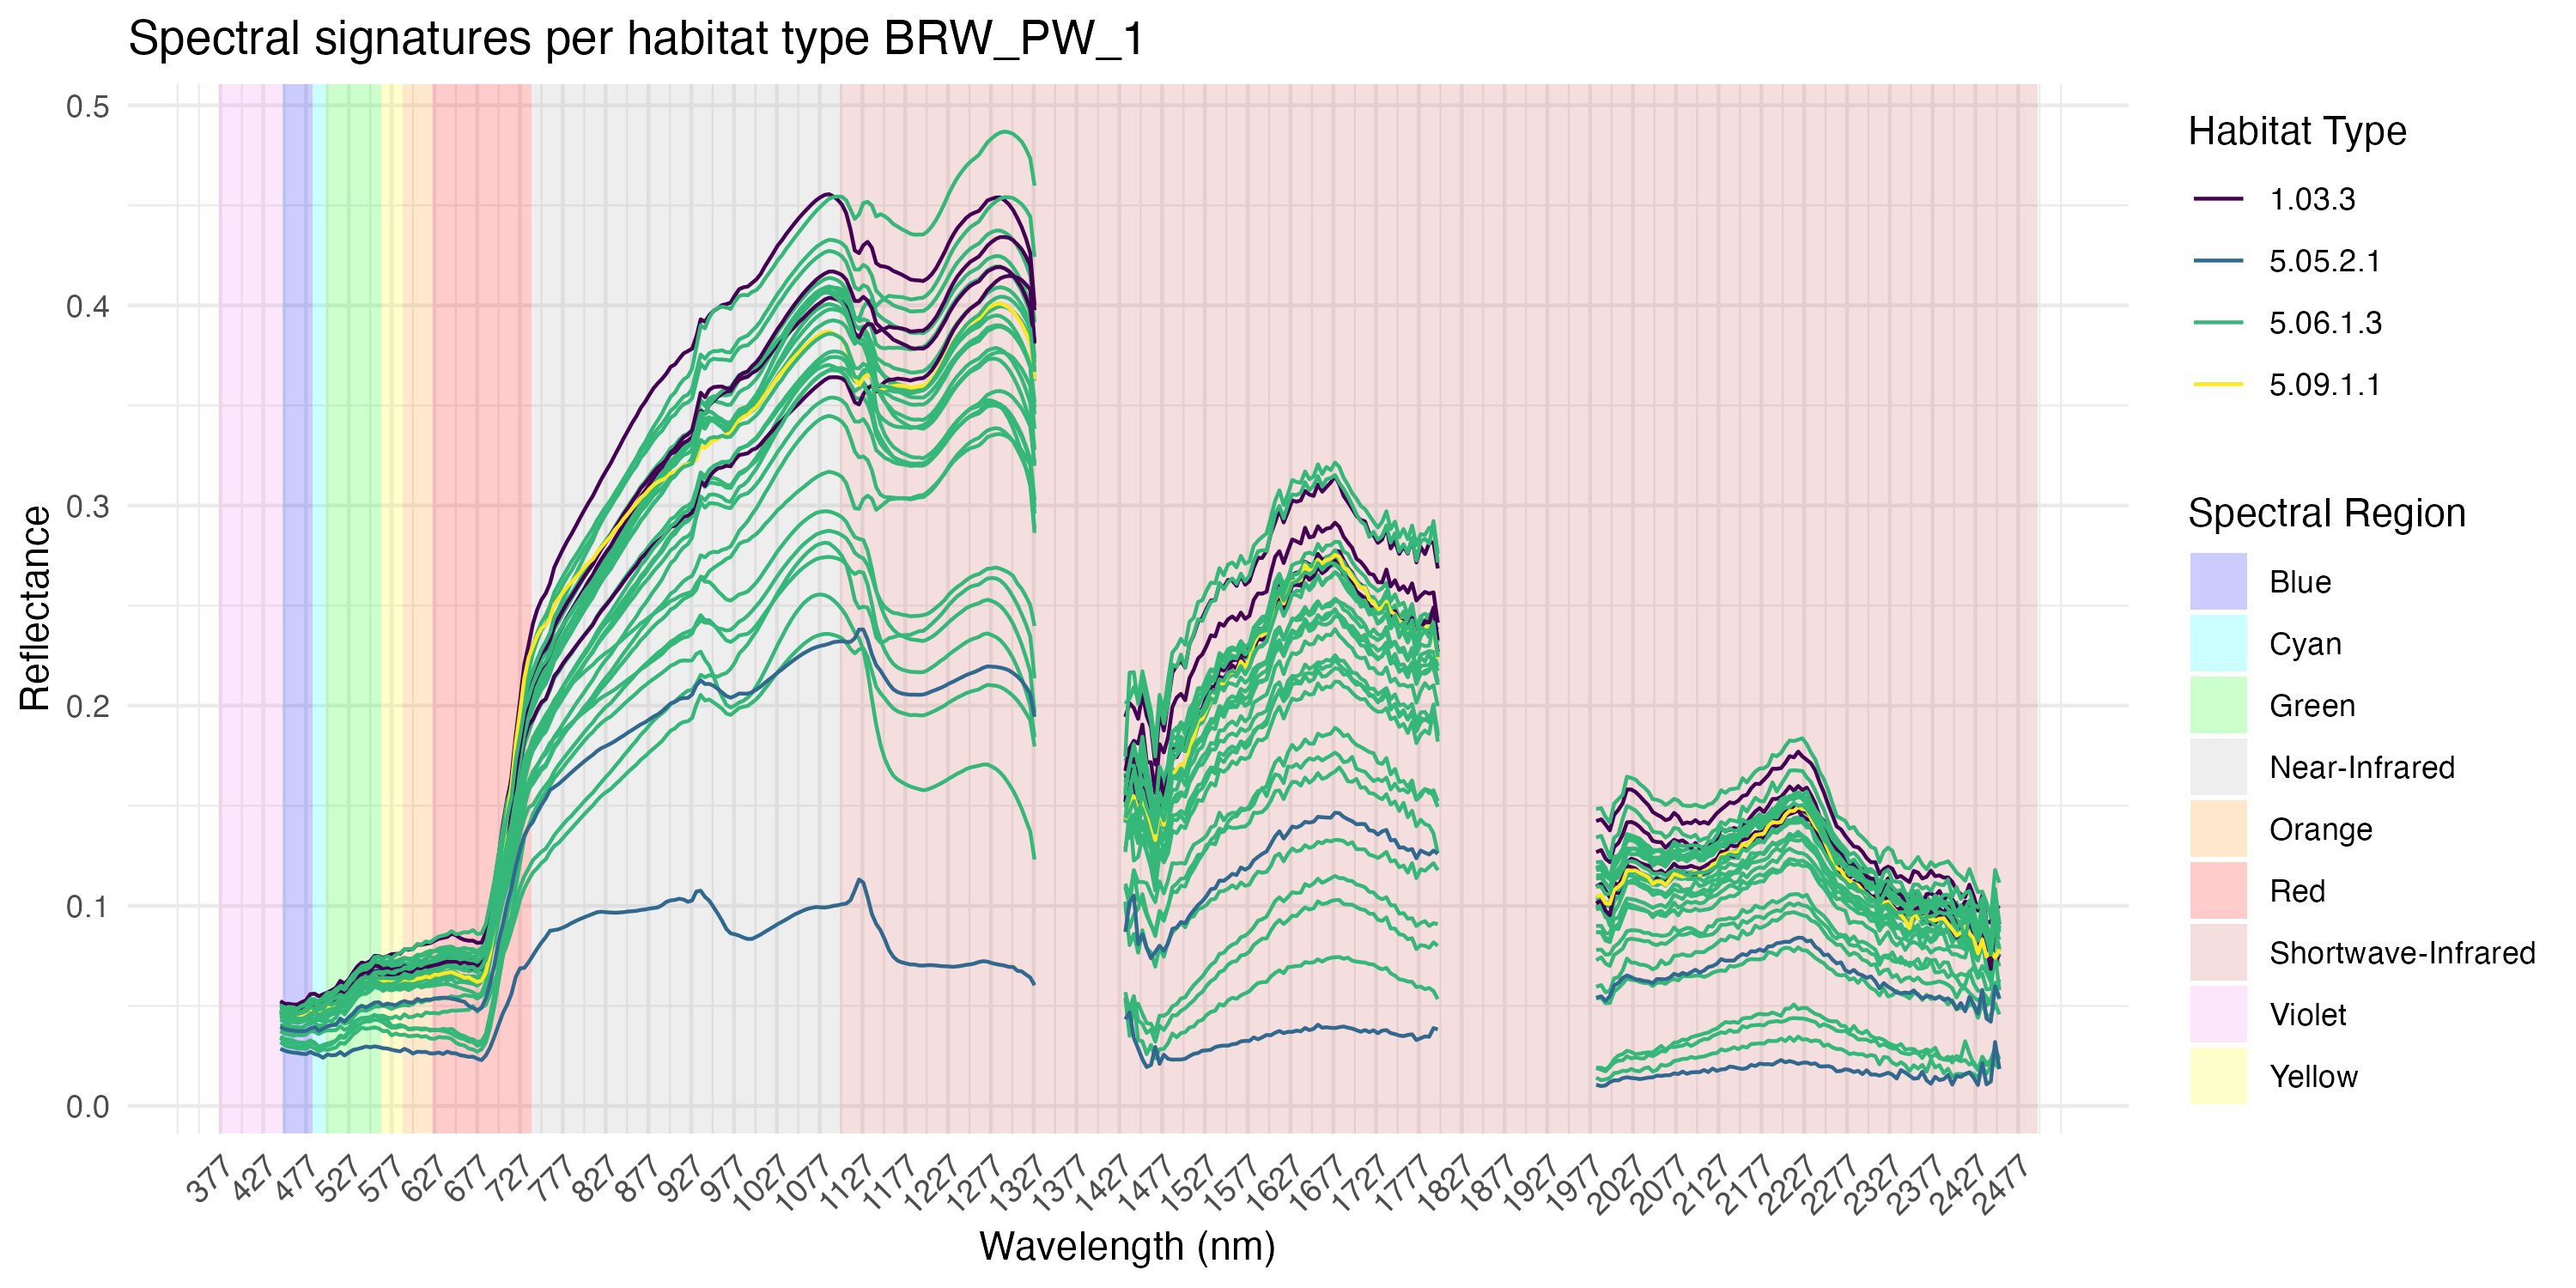
\includegraphics[width=\textwidth]{Figures/spectral_signatures/BRW_PW_1_signature_plot_habitat.png}
    \caption{}
    \label{fig:ss_ht_brwpw1}
  \end{subfigure}
  \hfill
  \begin{subfigure}[b]{0.49\textwidth}
    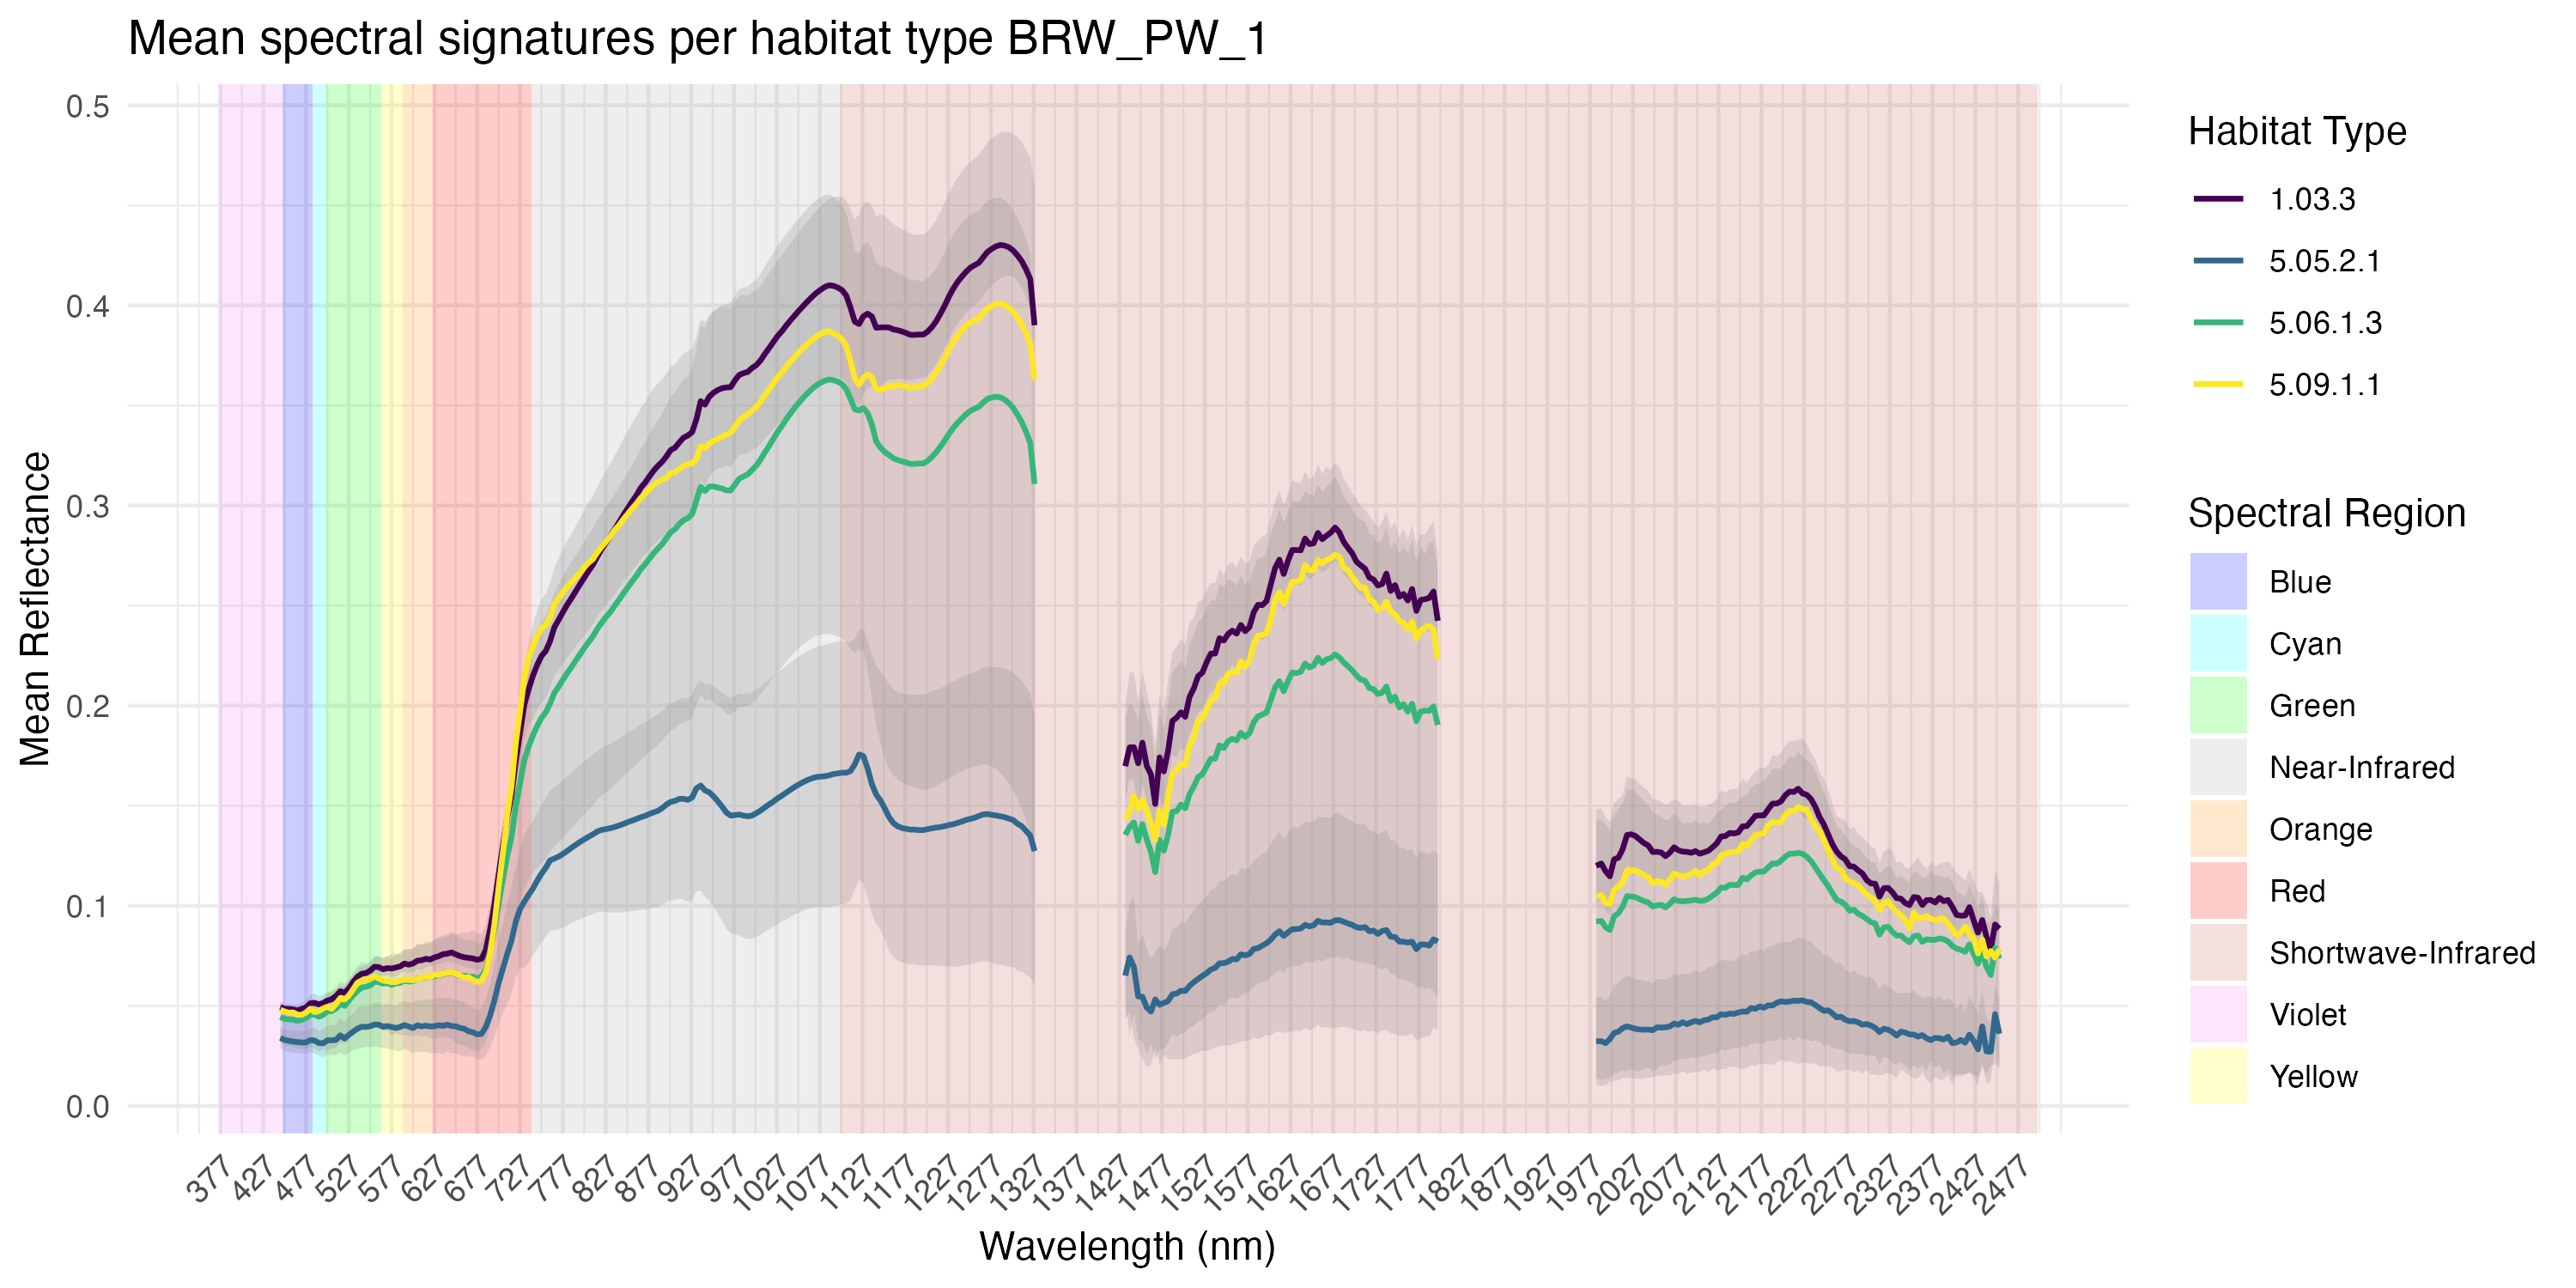
\includegraphics[width=\textwidth]{Figures/spectral_signatures/BRW_PW_1_mean_signature_plot_habitat.png}
    \caption{}
    \label{fig:mss_ht_brwpw1}
  \end{subfigure}

  \caption{Spectral signature plot \ref{fig:ss_ht_brwpw1} and mean spectral signature plot \ref{fig:mss_ht_brwpw1} grouped by habitat type for test site BRW\_PW\_1}
  \label{fig:group_ss_ht_brwpw1}
\end{figure}

\begin{figure}[H]
  \centering

  \begin{subfigure}[b]{0.49\textwidth}
    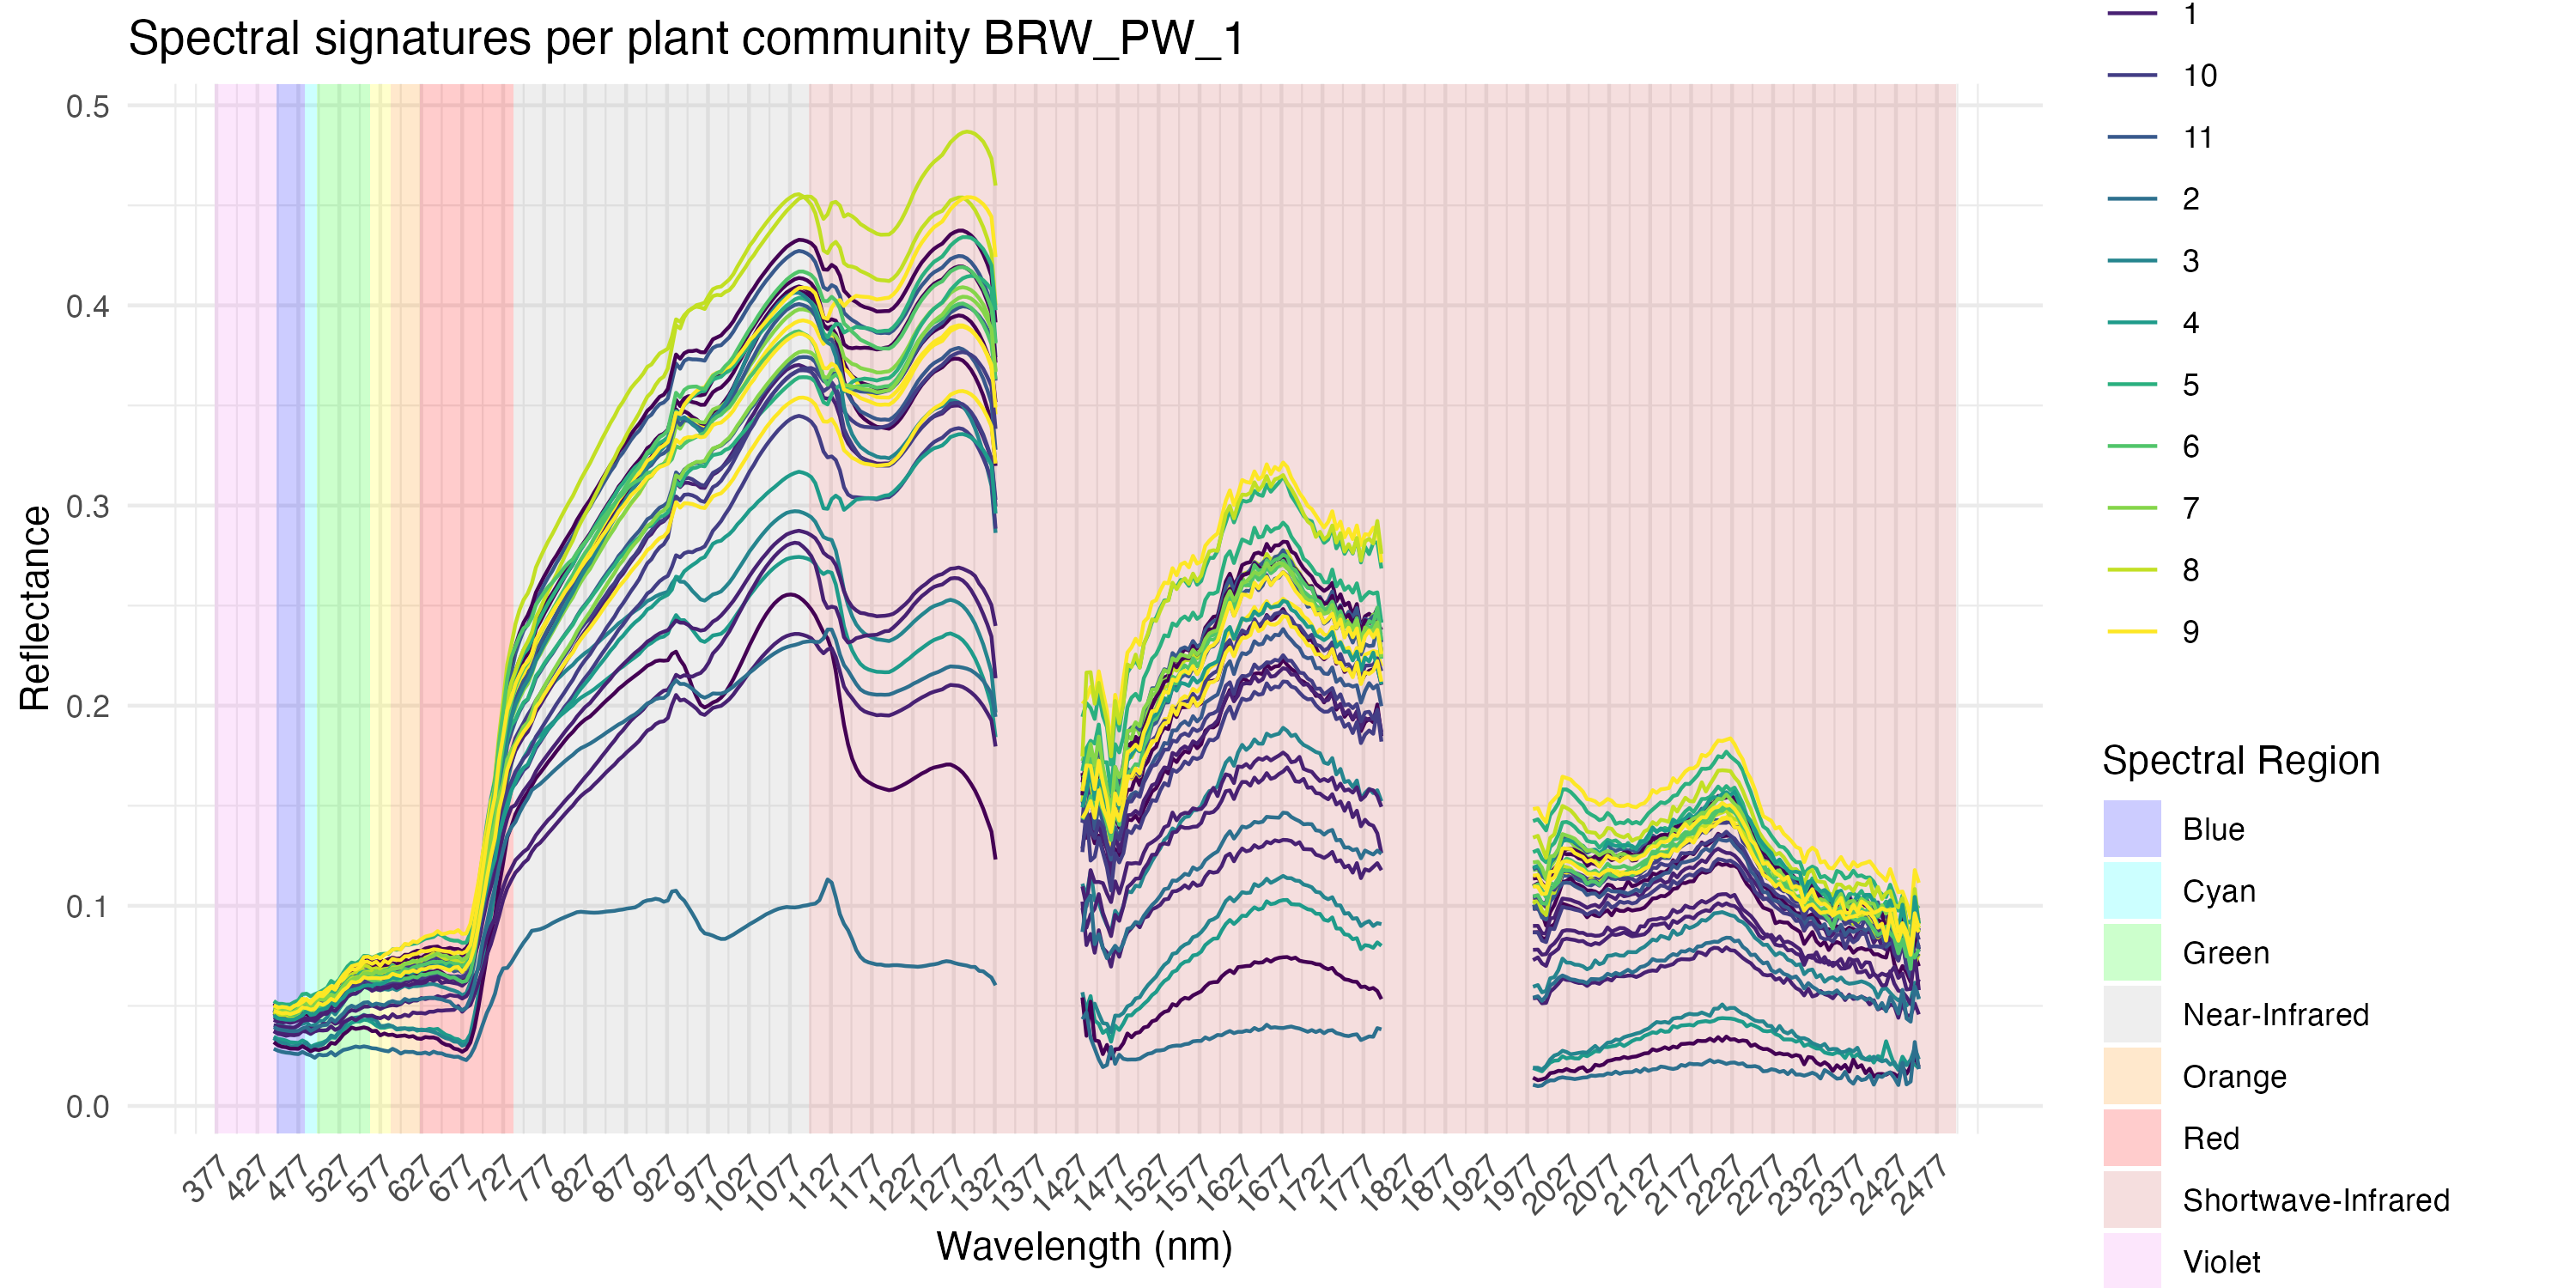
\includegraphics[width=\textwidth]{Figures/spectral_signatures/BRW_PW_1_signature_plot_plant_community.png}
    \caption{}
    \label{fig:ss_pc_brwpw1}
  \end{subfigure}
  \hfill
  \begin{subfigure}[b]{0.49\textwidth}
    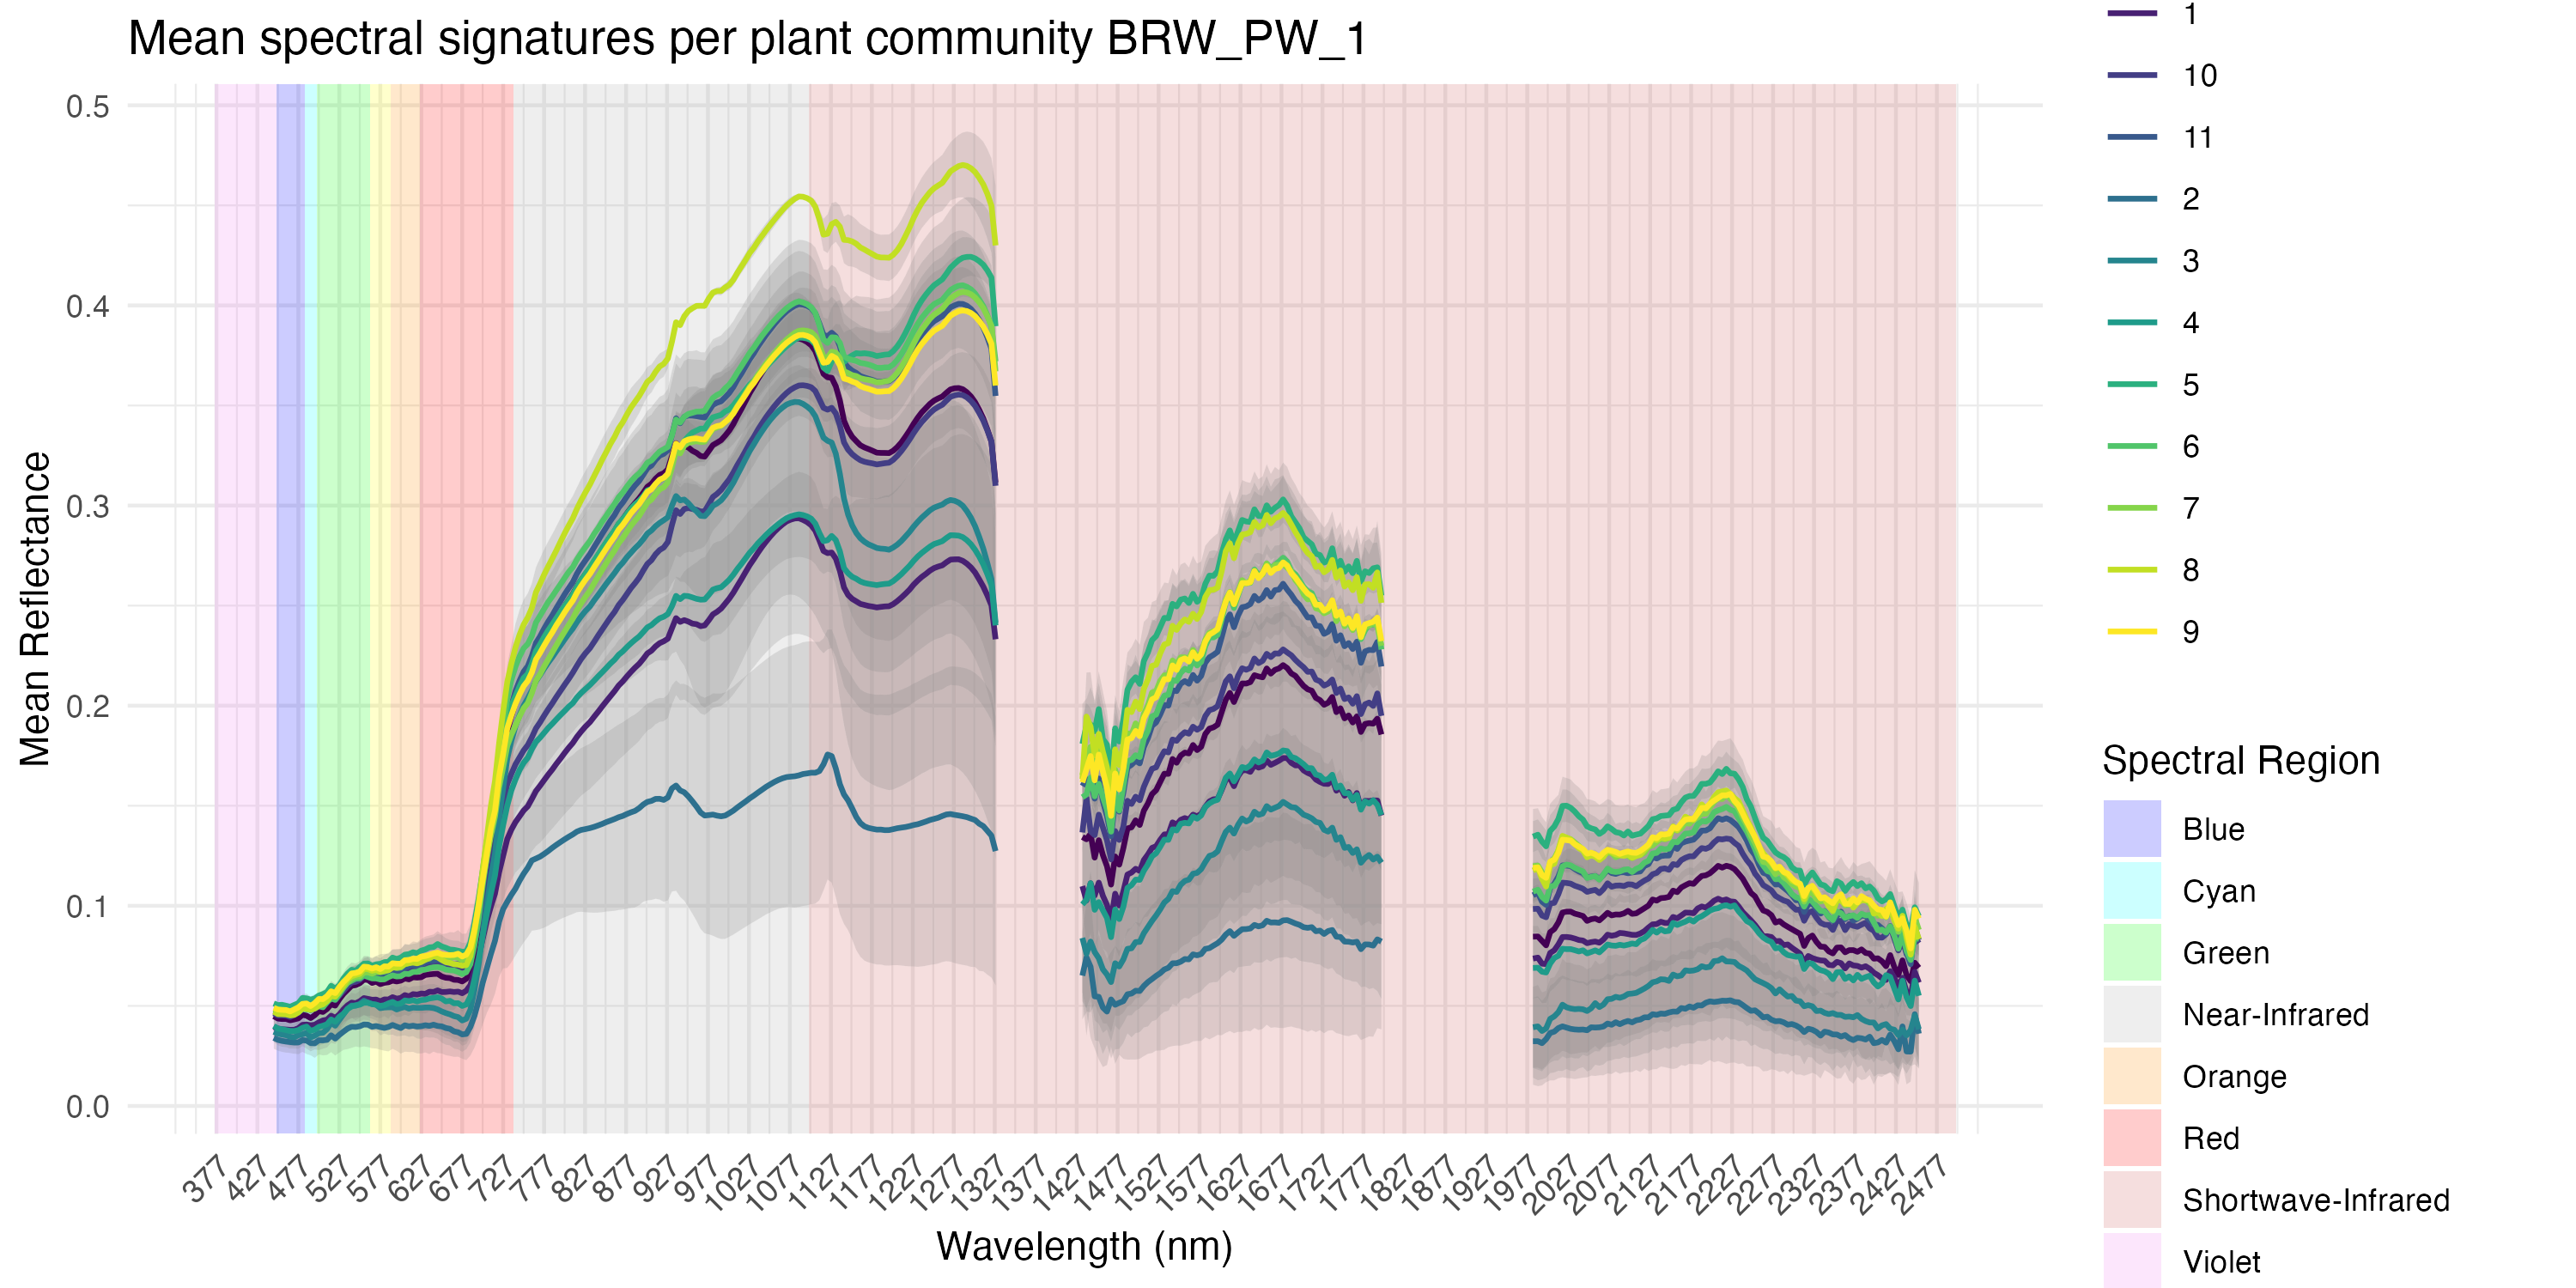
\includegraphics[width=\textwidth]{Figures/spectral_signatures/BRW_PW_1_mean_signature_plot_plant_community.png}
    \caption{}
    \label{fig:mss_pc_brwpw1}
  \end{subfigure}

  \caption{Spectral signature plot \ref{fig:ss_pc_brwpw1} and mean spectral signature plot \ref{fig:mss_pc_brwpw1} grouped by plant community cluster for test site BRW\_PW\_1}
  \label{fig:group_pc_ht_brwpw1}
\end{figure}

\subsection{BRW\_VS\_1}

\begin{figure}[H]
  \centering

  \begin{subfigure}[b]{0.49\textwidth}
    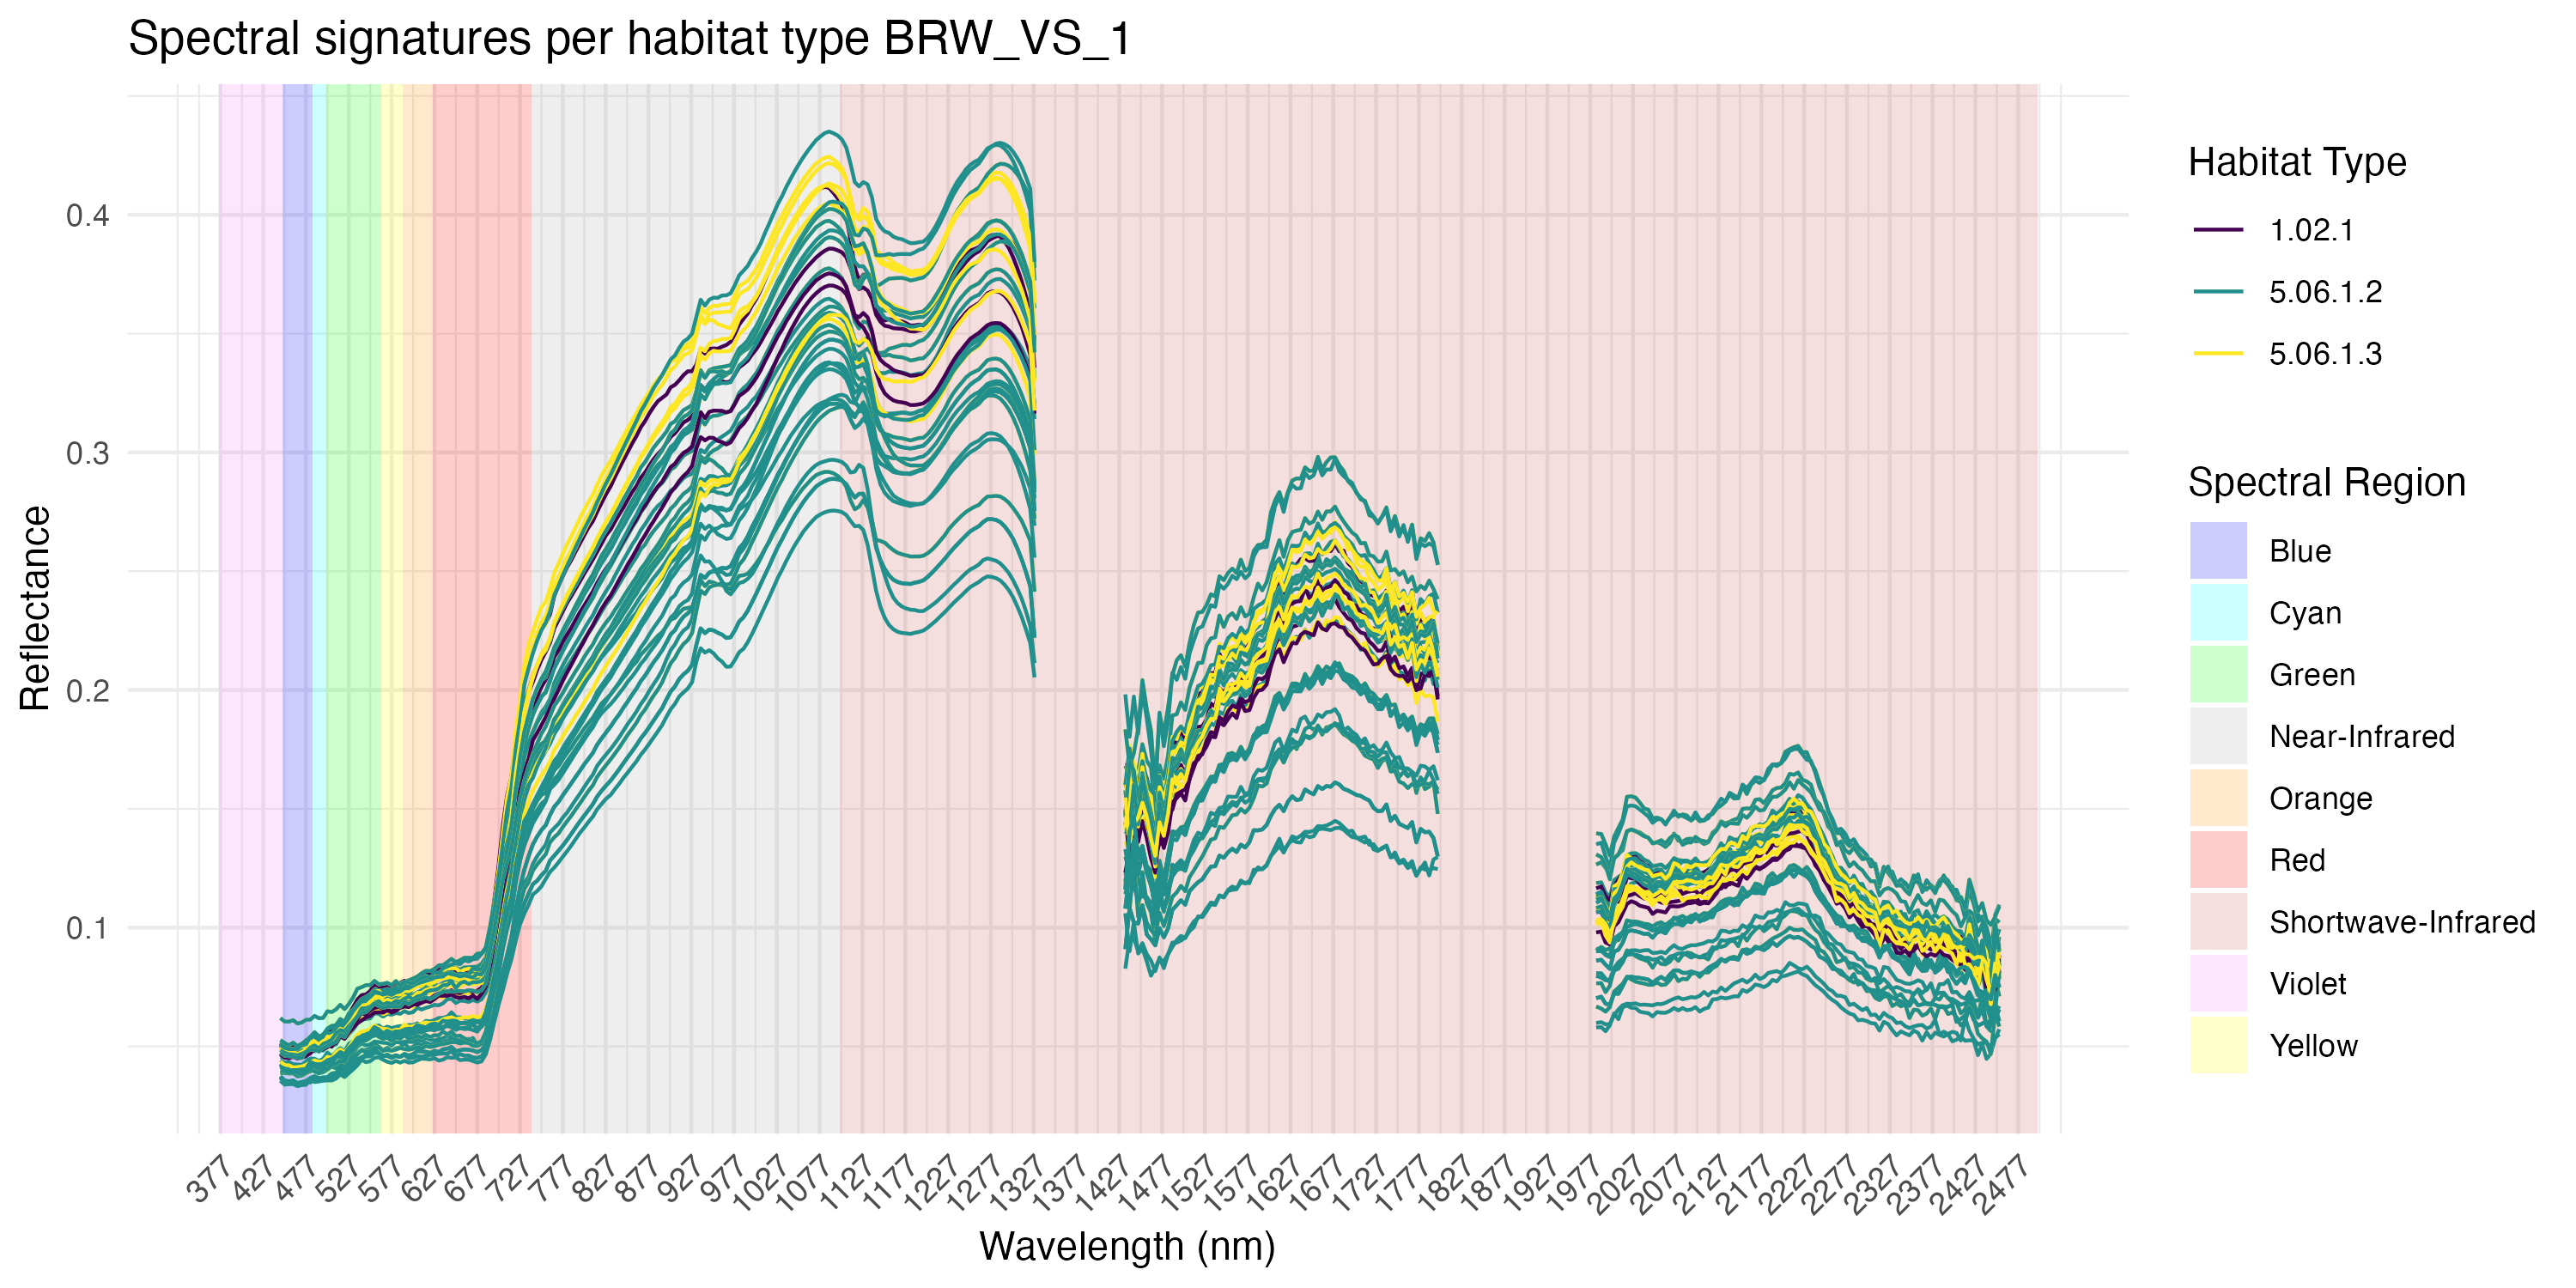
\includegraphics[width=\textwidth]{Figures/spectral_signatures/BRW_VS_1_signature_plot_habitat.png}
    \caption{}
    \label{fig:ss_ht_brwvs1}
  \end{subfigure}
  \hfill
  \begin{subfigure}[b]{0.49\textwidth}
    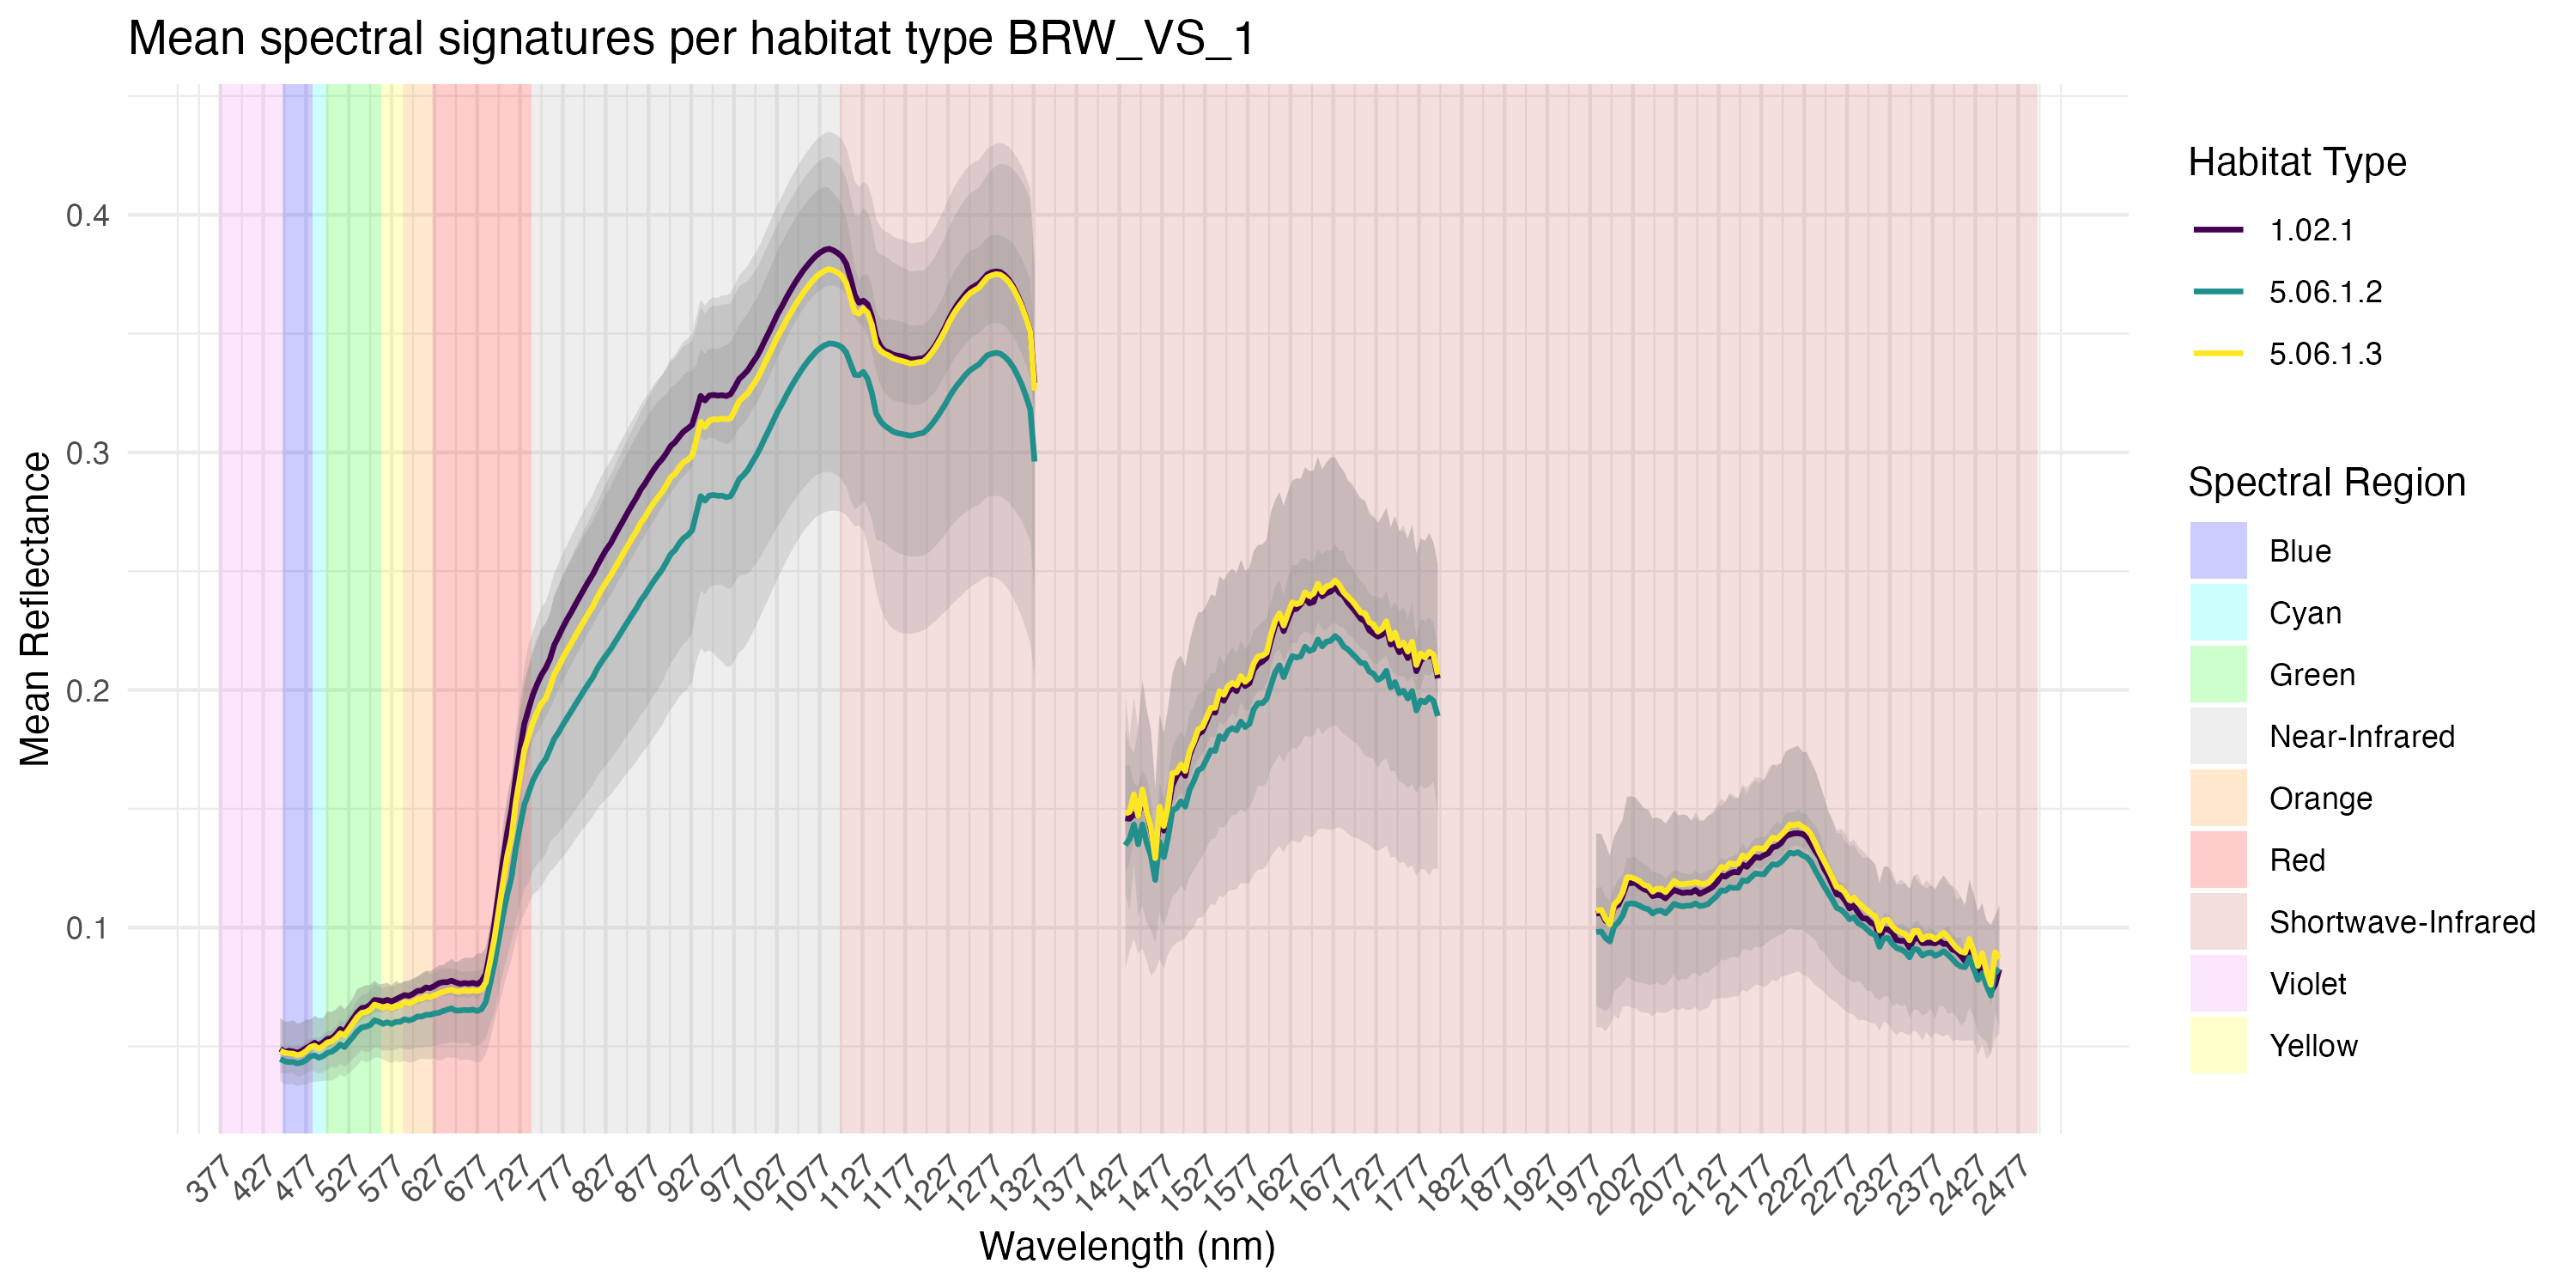
\includegraphics[width=\textwidth]{Figures/spectral_signatures/BRW_VS_1_mean_signature_plot_habitat.png}
    \caption{}
    \label{fig:mss_ht_brwvs1}
  \end{subfigure}

  \caption{Spectral signature plot \ref{fig:ss_ht_brwvs1} and mean spectral signature plot \ref{fig:mss_ht_brwvs1} grouped by habitat type for test site BRW\_VS\_1}
  \label{fig:group_ss_ht_brwvs1}
\end{figure}

\begin{figure}[H]
  \centering

  \begin{subfigure}[b]{0.49\textwidth}
    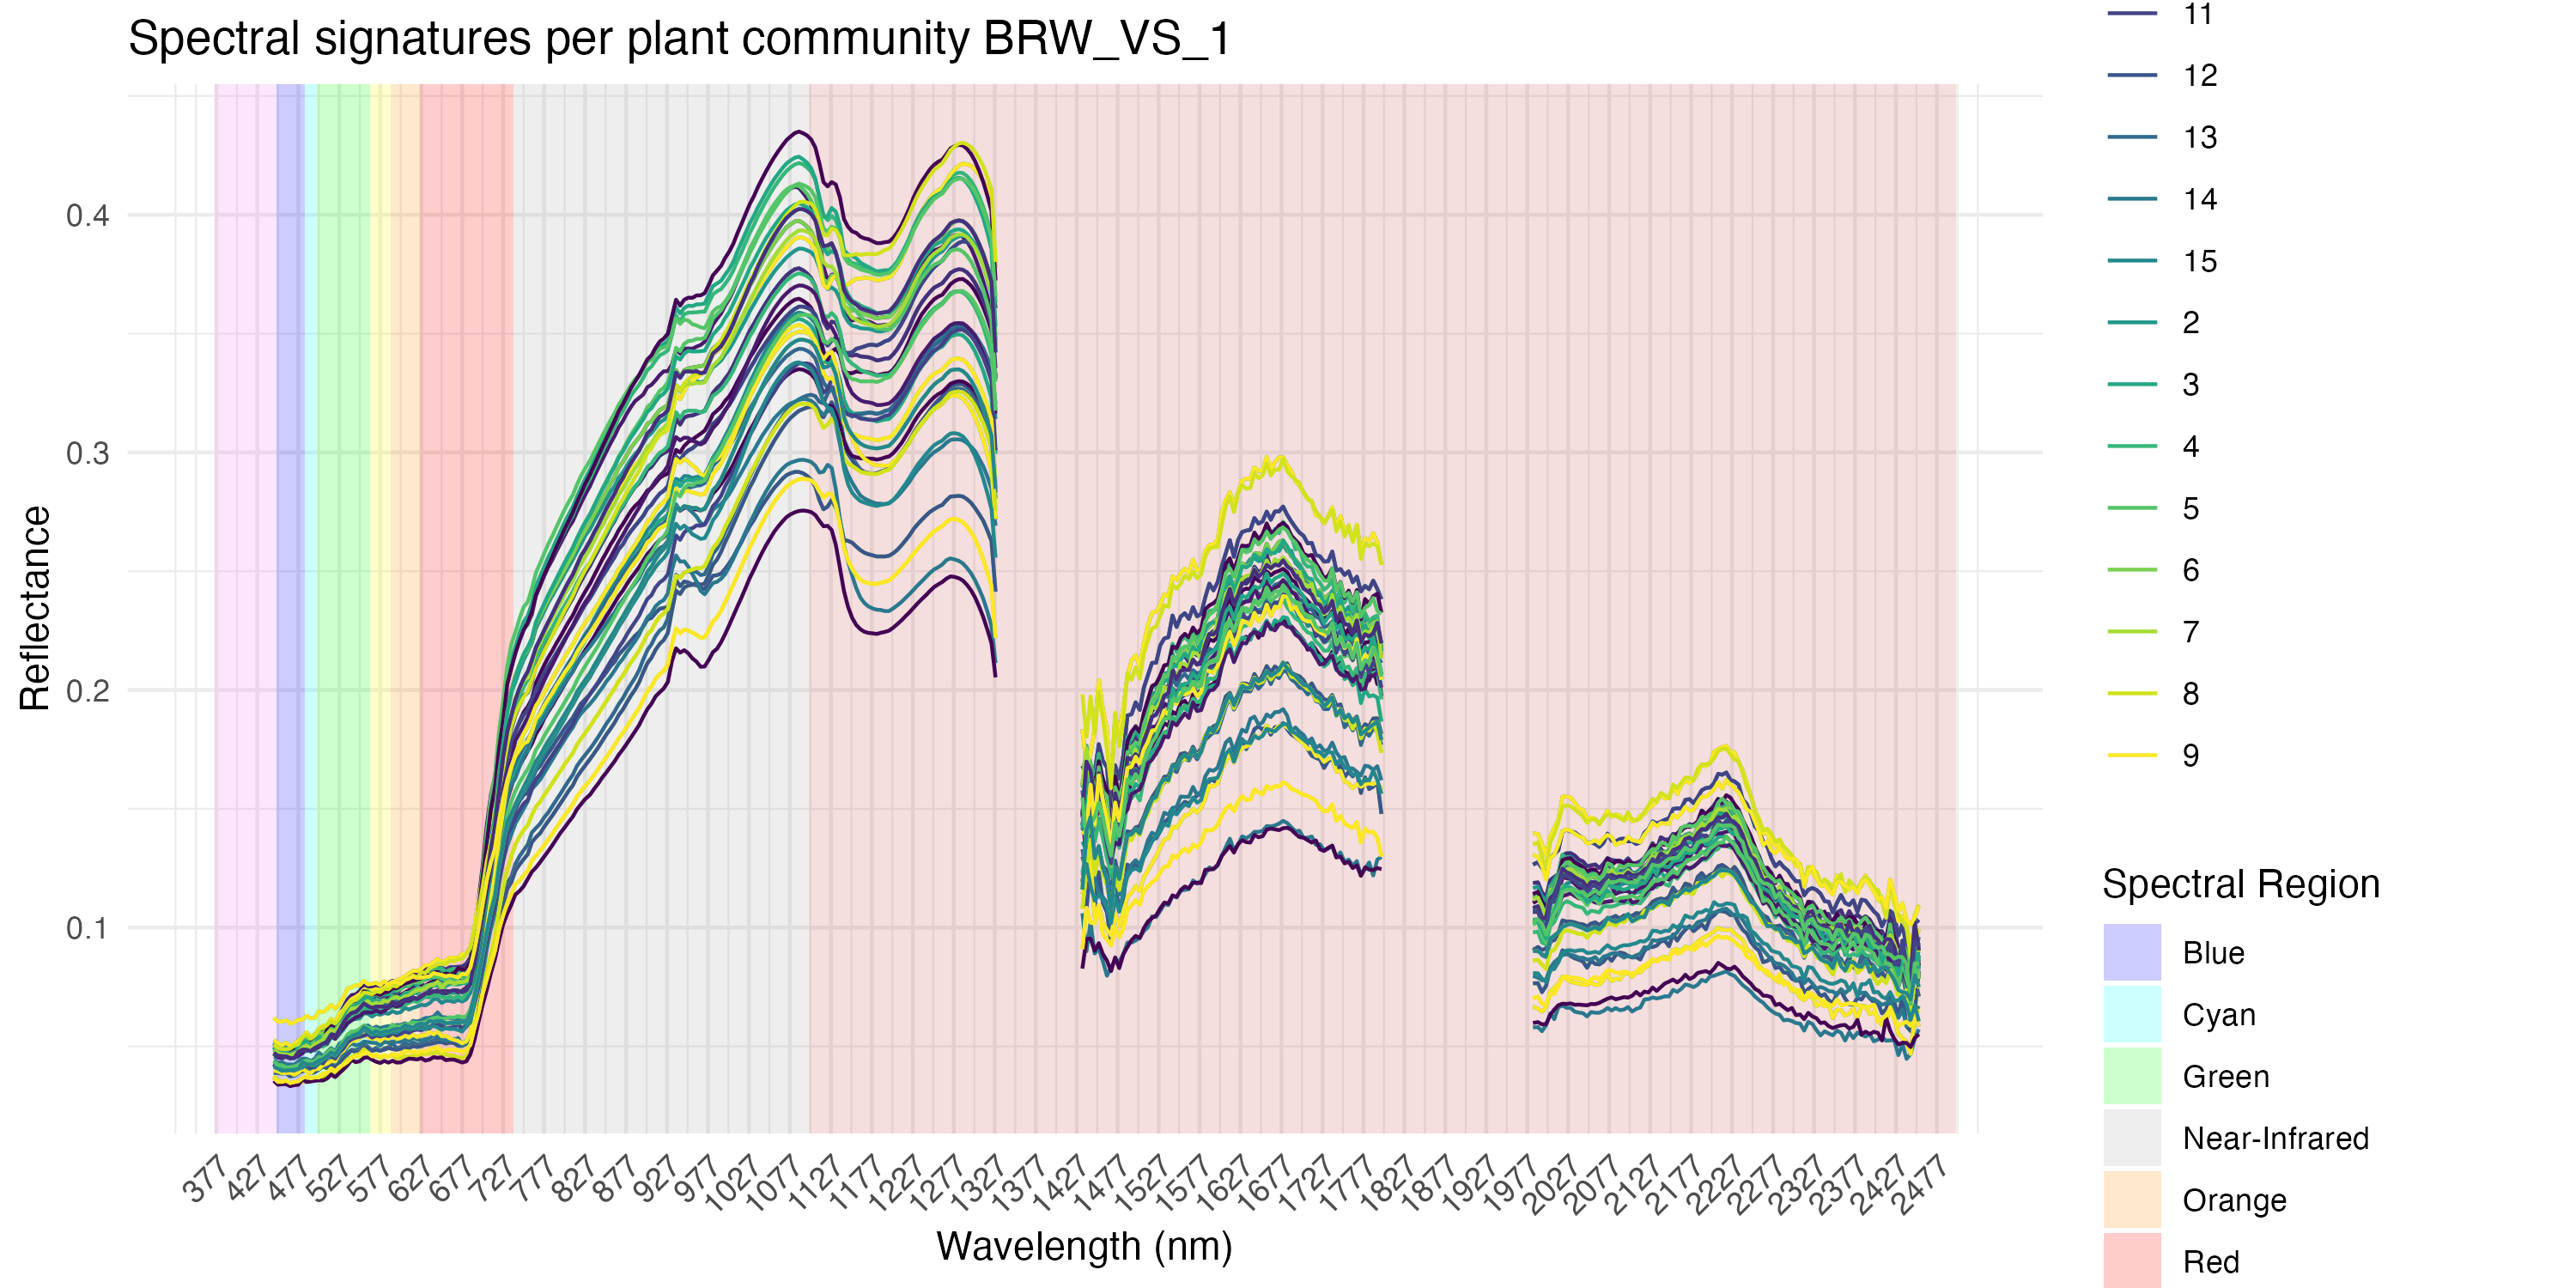
\includegraphics[width=\textwidth]{Figures/spectral_signatures/BRW_VS_1_signature_plot_plant_community.png}
    \caption{}
    \label{fig:ss_pc_brwvs1}
  \end{subfigure}
  \hfill
  \begin{subfigure}[b]{0.49\textwidth}
    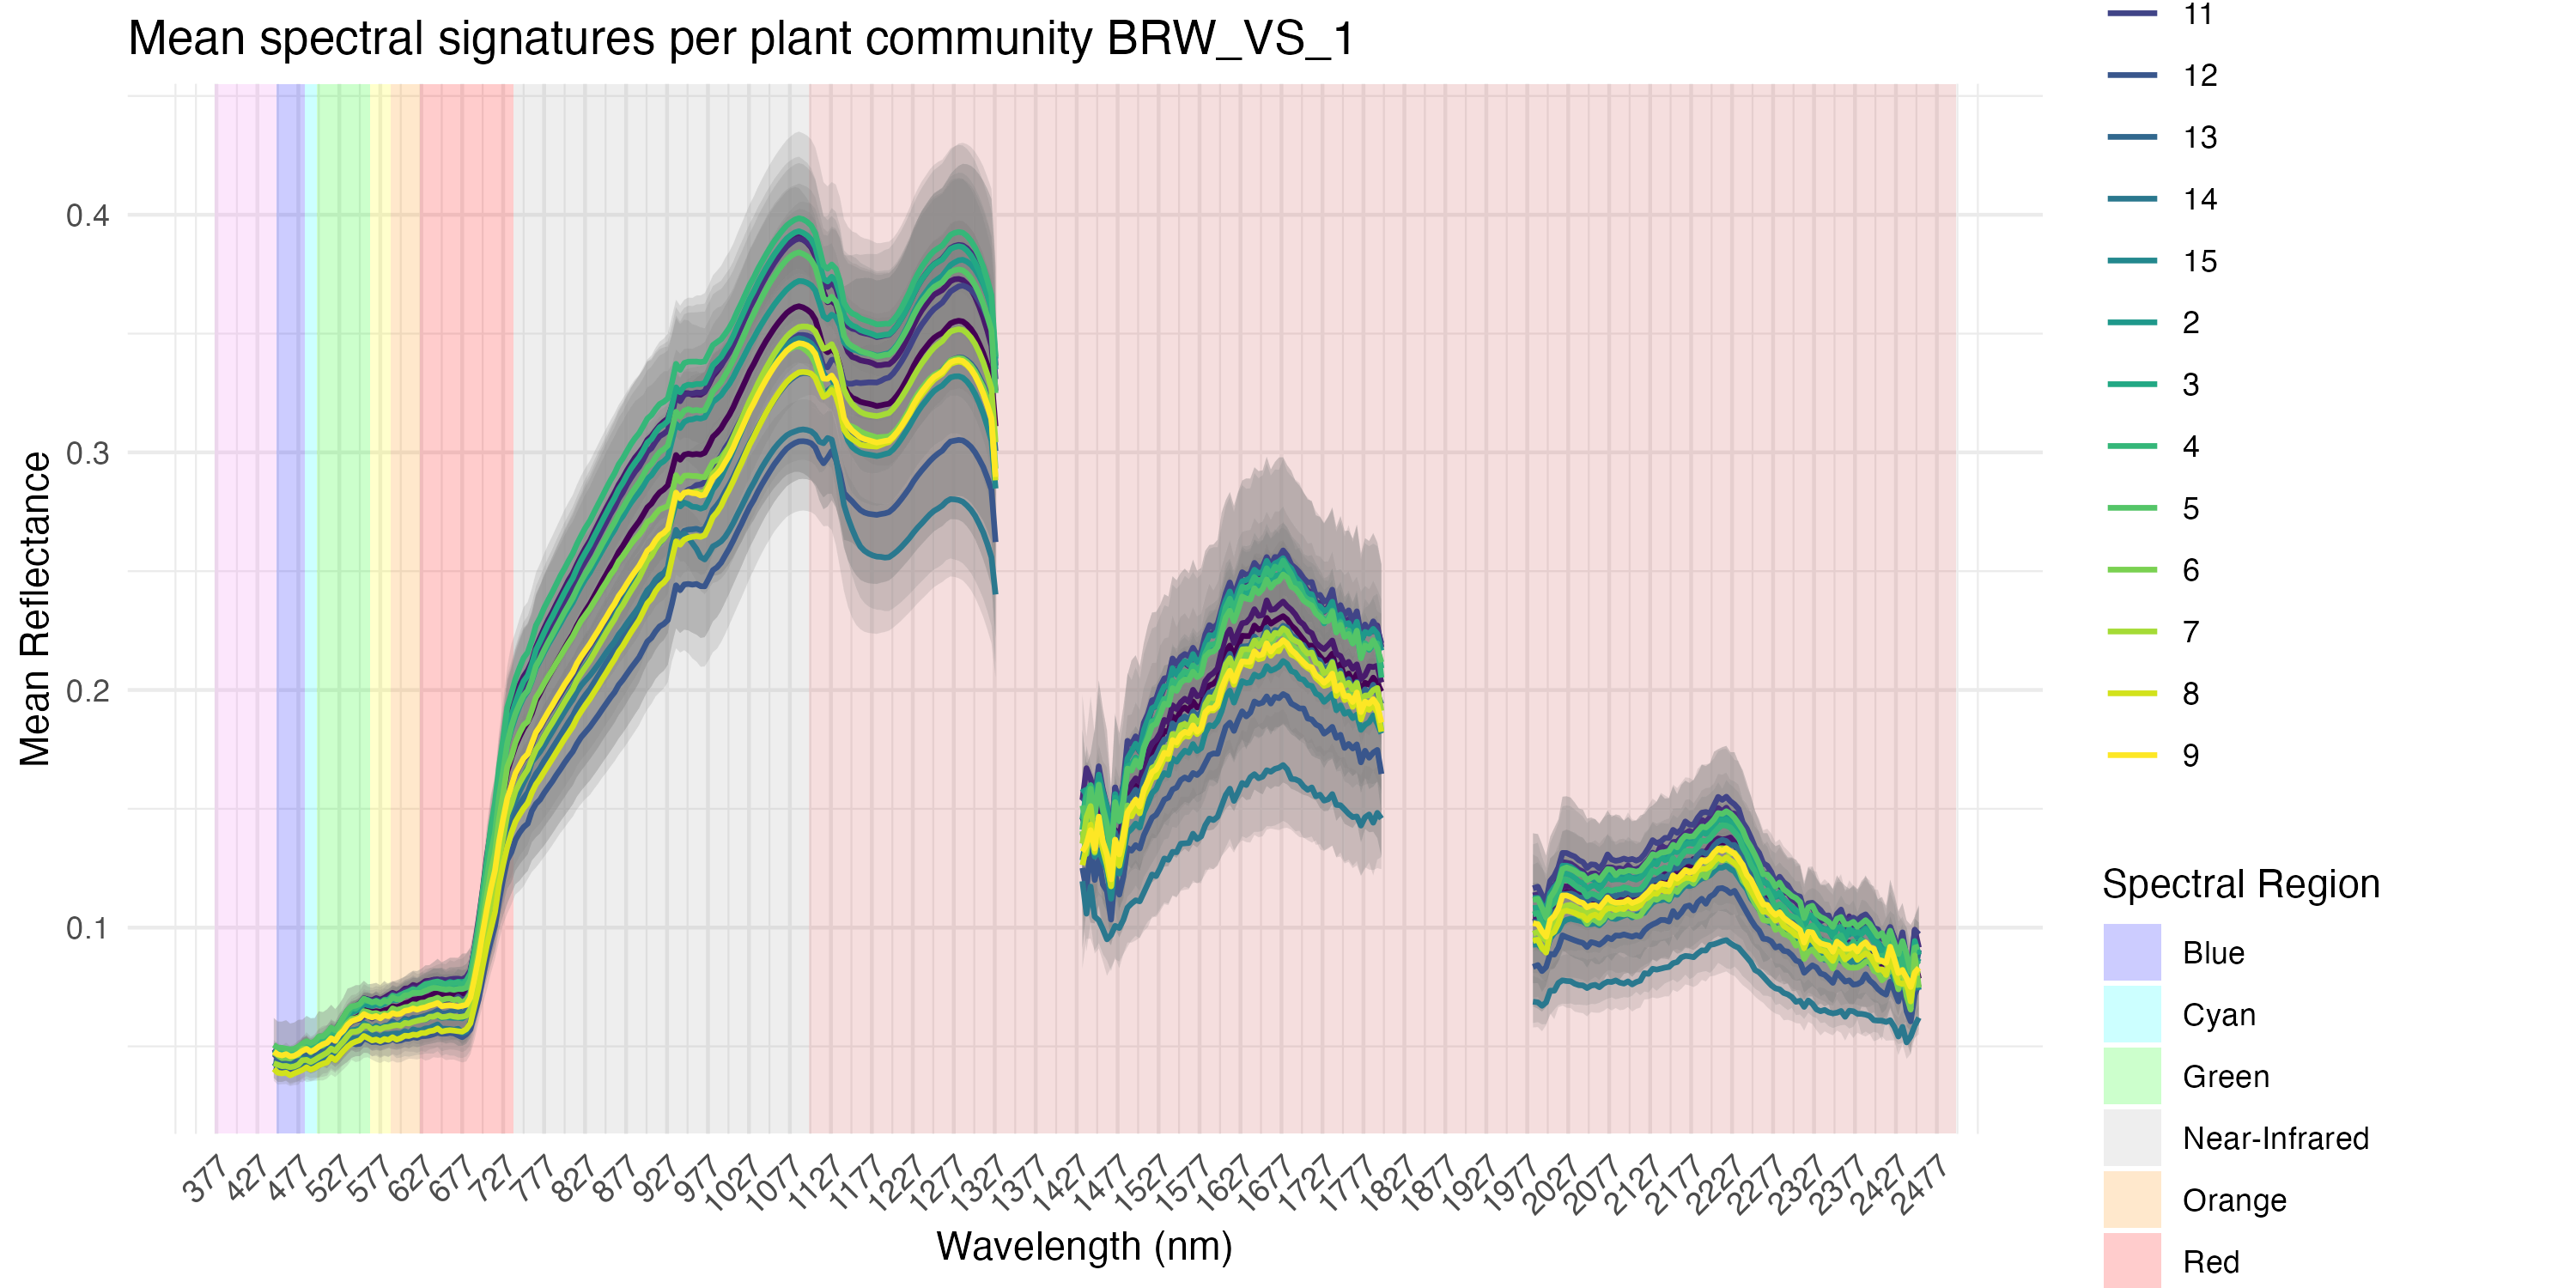
\includegraphics[width=\textwidth]{Figures/spectral_signatures/BRW_VS_1_mean_signature_plot_plant_community.png}
    \caption{}
    \label{fig:mss_pc_brwvs1}
  \end{subfigure}

  \caption{Spectral signature plot \ref{fig:ss_pc_brwvs1} and mean spectral signature plot \ref{fig:mss_pc_brwvs1} grouped by plant community cluster for test site BRW\_VS\_1}
  \label{fig:group_pc_ht_brwvs1}
\end{figure}

\subsection{FLXTWRZONA\_SD\_1}

\begin{figure}[H]
  \centering

  \begin{subfigure}[b]{0.49\textwidth}
    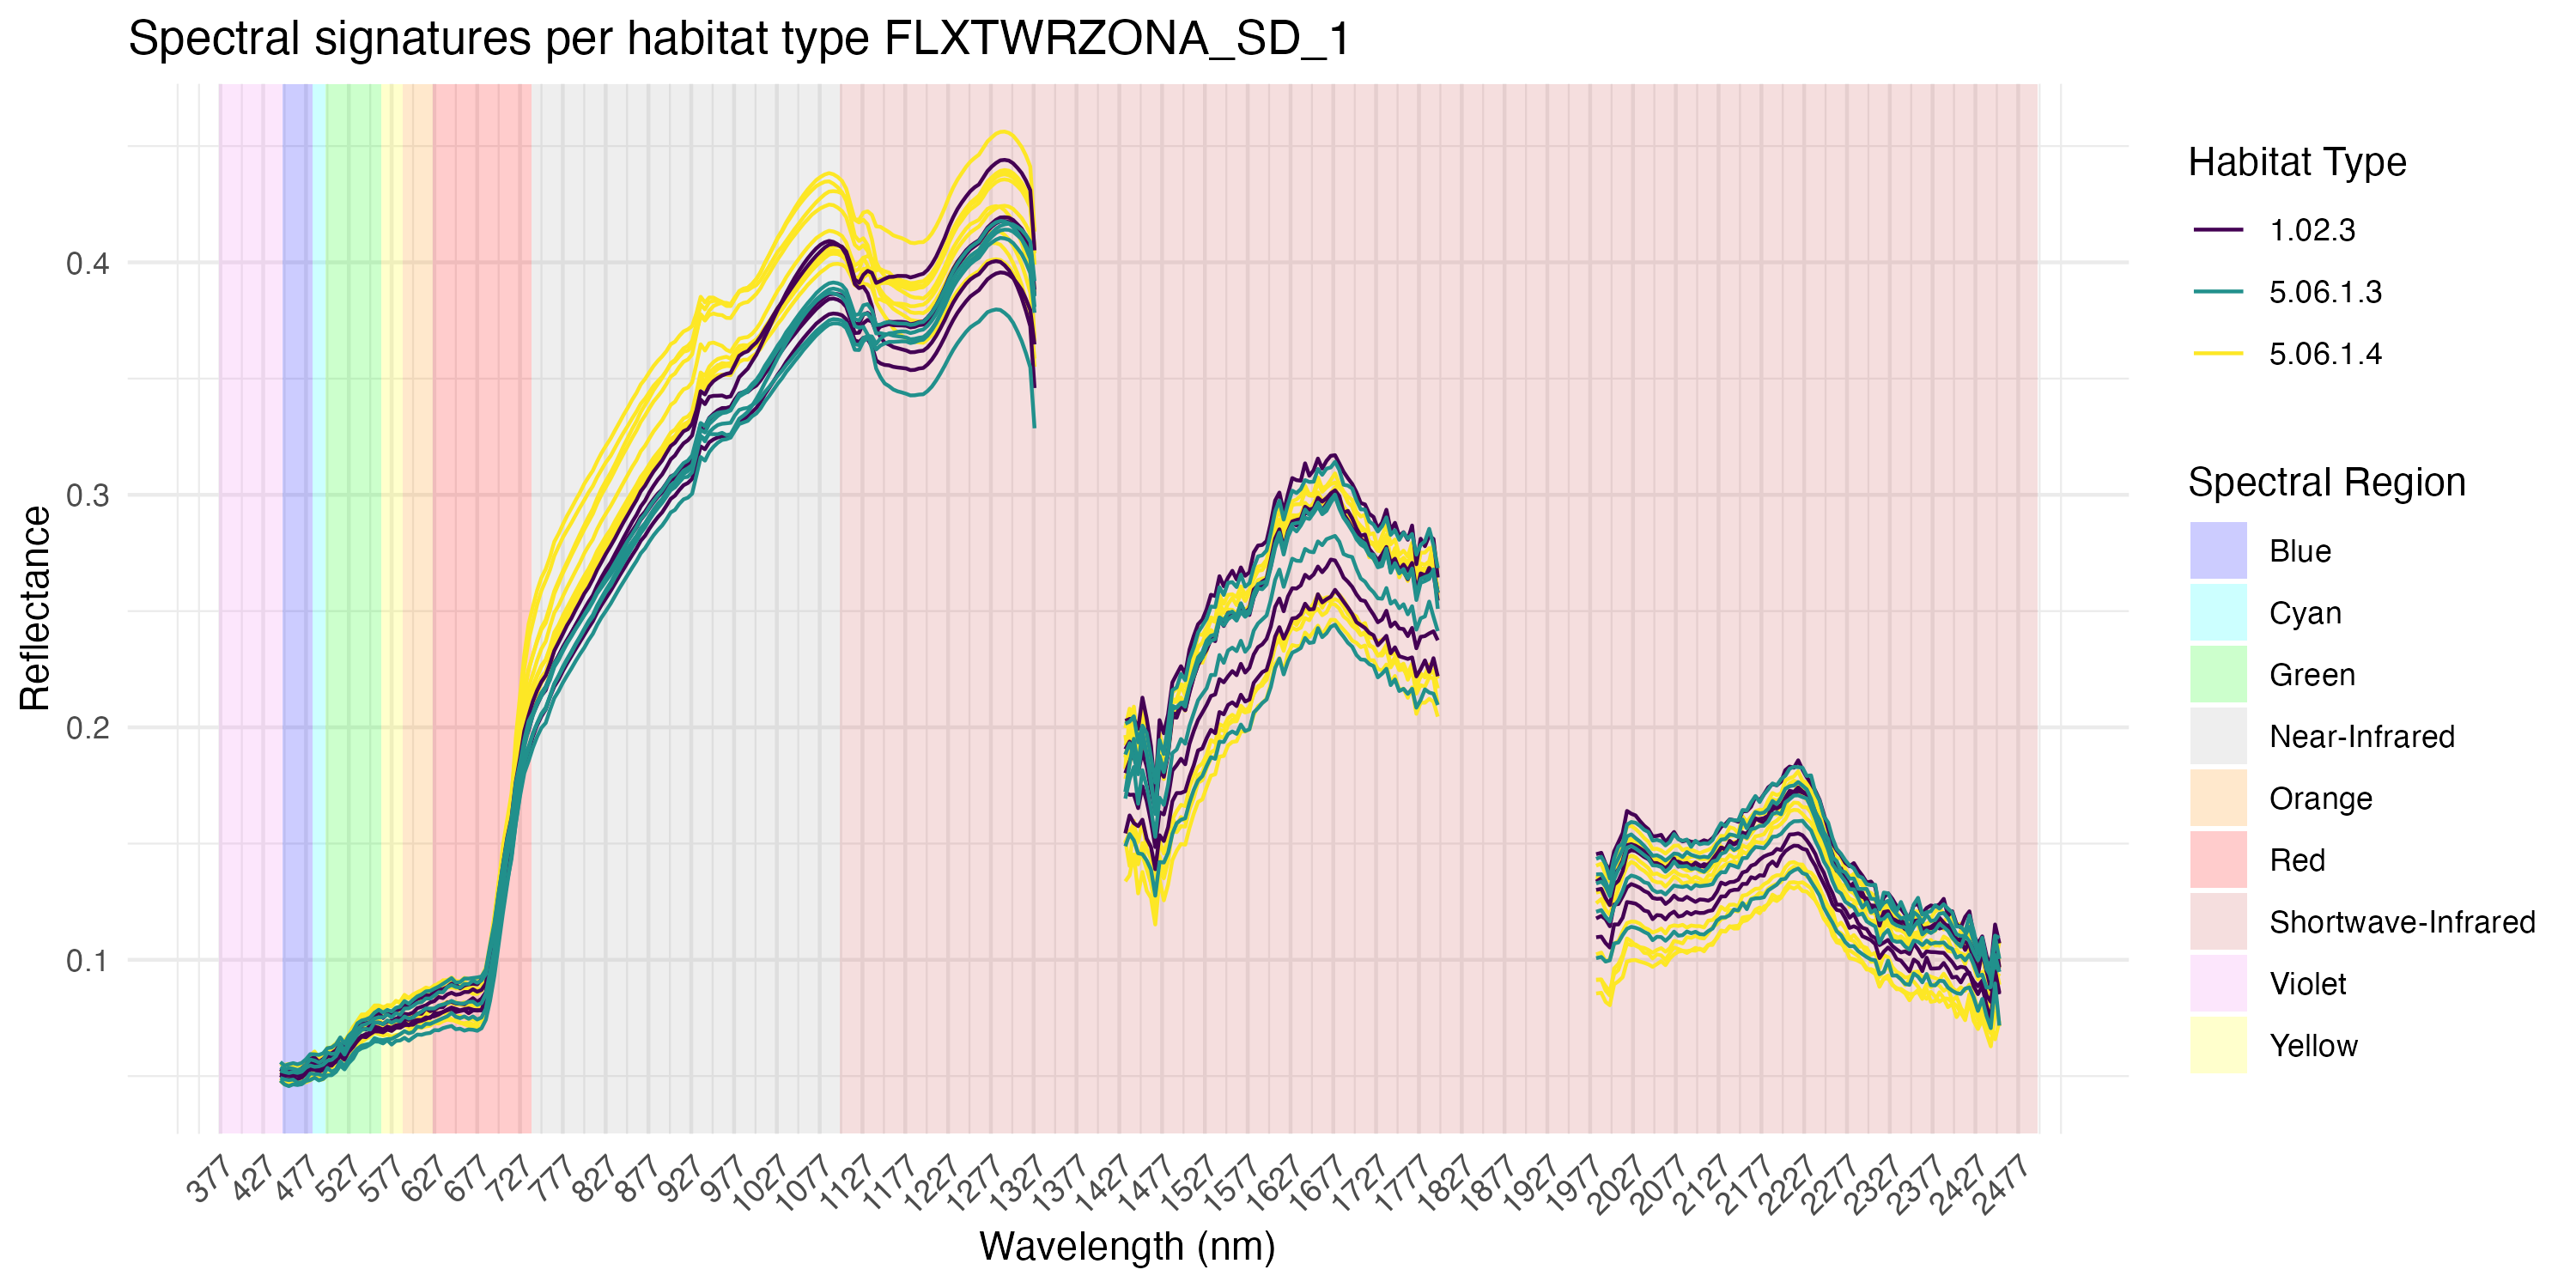
\includegraphics[width=\textwidth]{Figures/spectral_signatures/FLXTWRZONA_SD_1_signature_plot_habitat.png}
    \caption{}
    \label{fig:ss_ht_flxtwrzonasd1}
  \end{subfigure}
  \hfill
  \begin{subfigure}[b]{0.49\textwidth}
    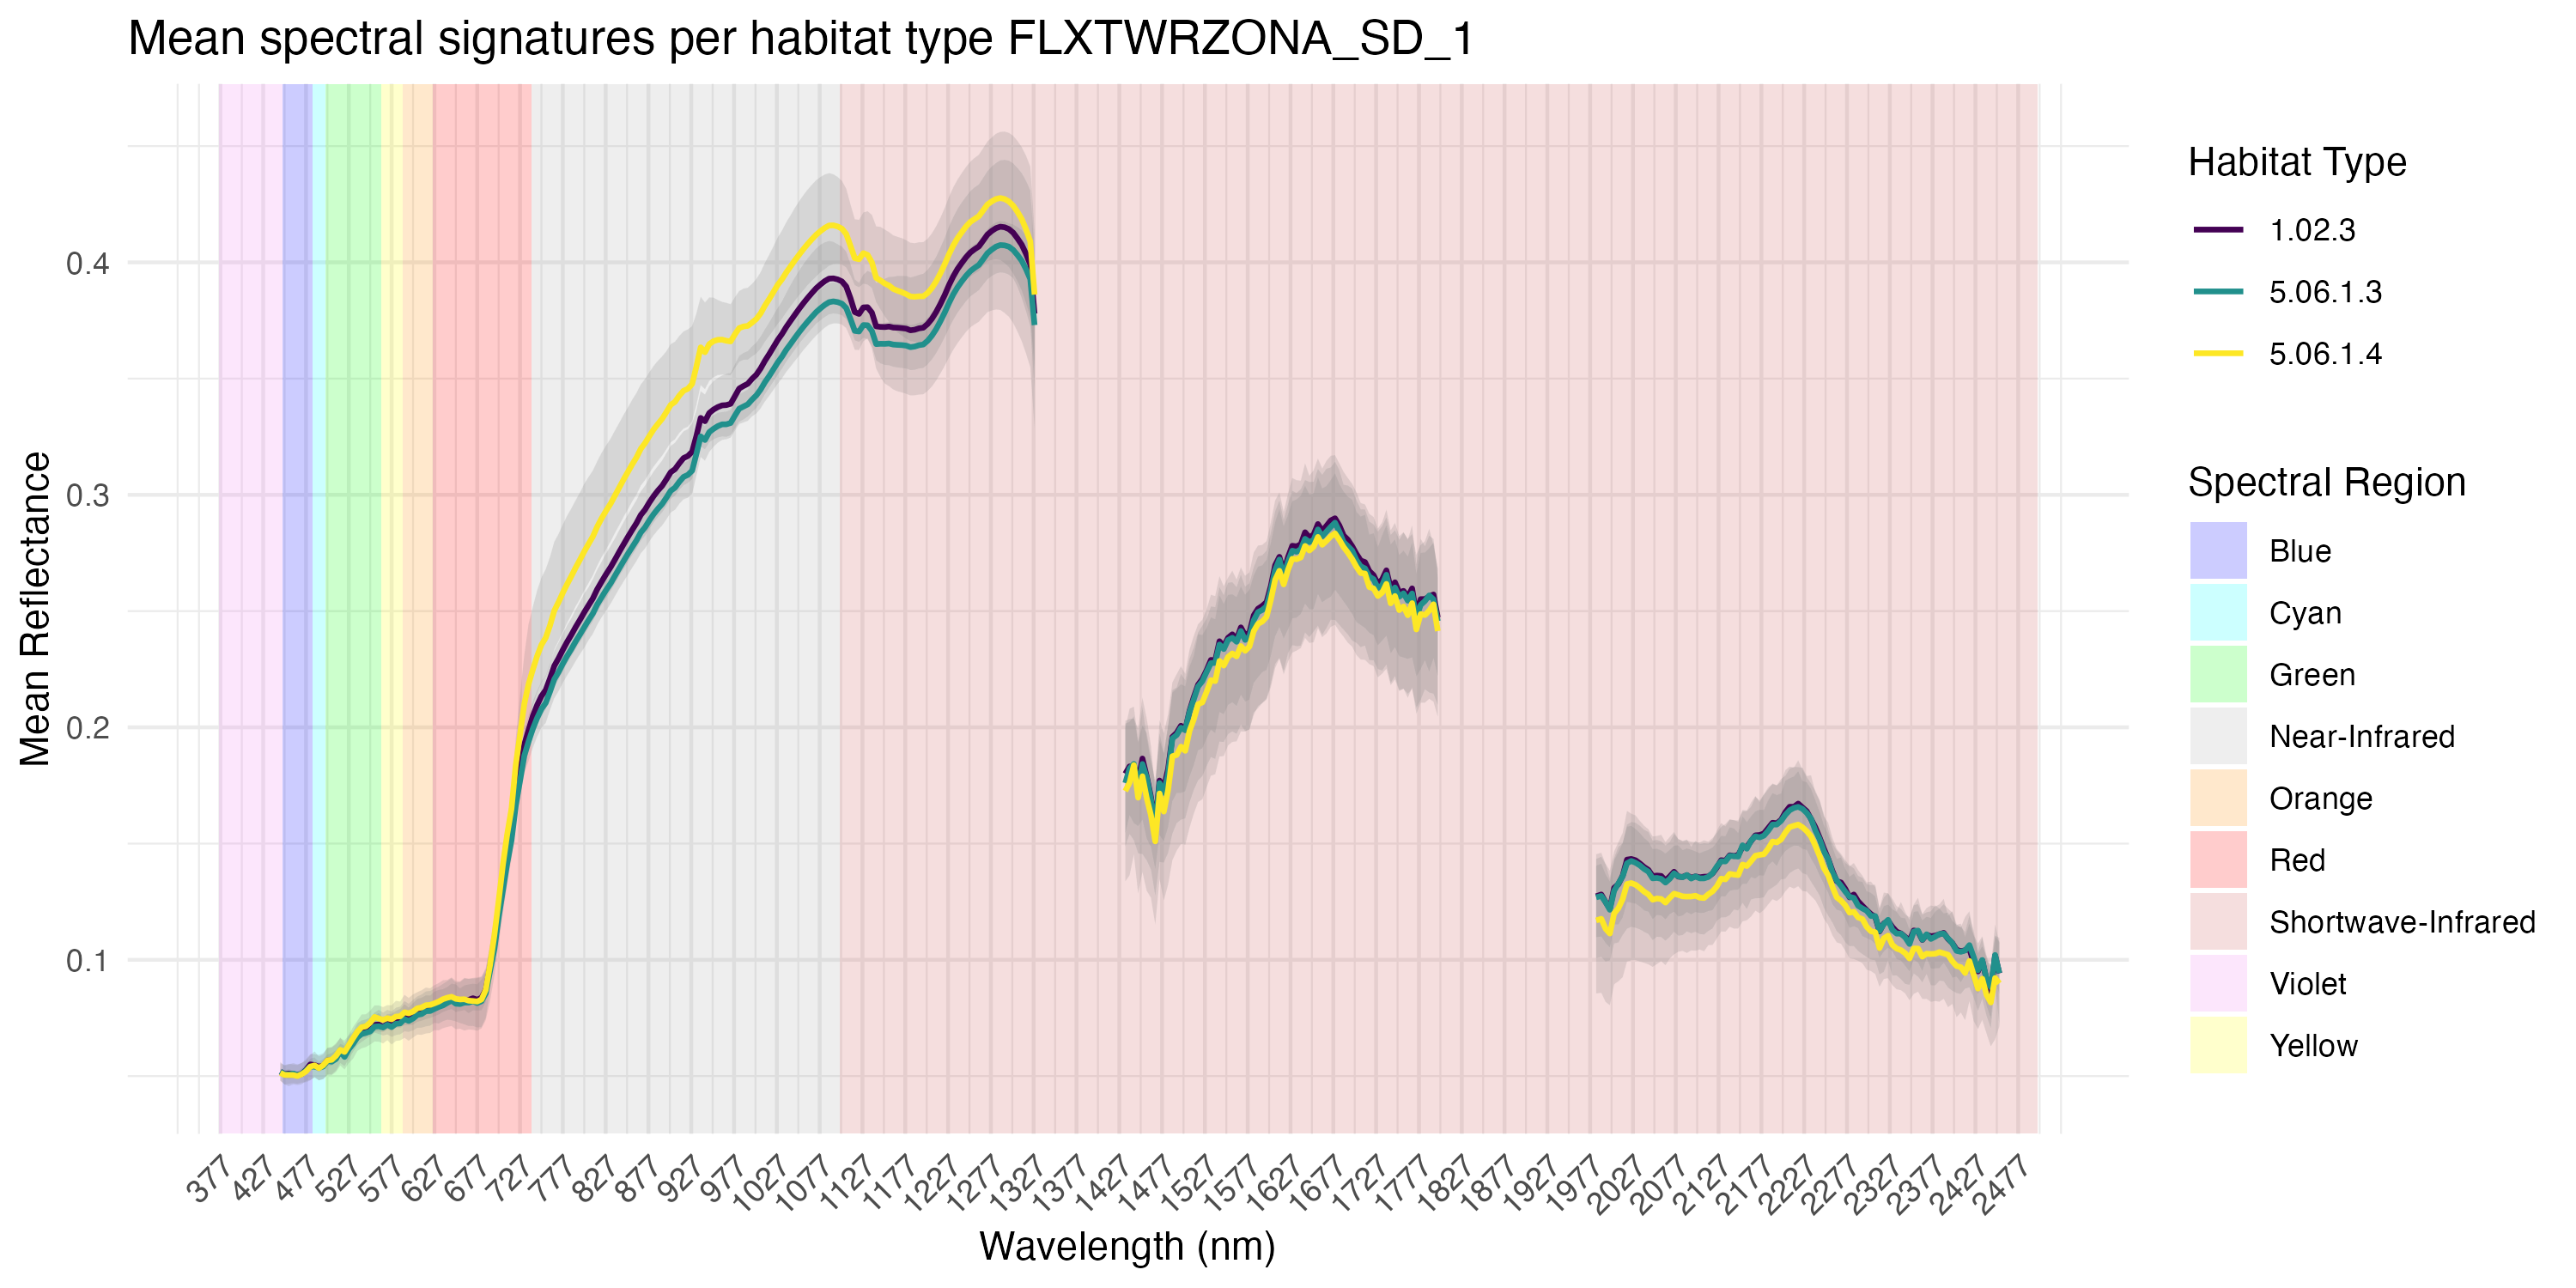
\includegraphics[width=\textwidth]{Figures/spectral_signatures/FLXTWRZONA_SD_1_mean_signature_plot_habitat.png}
    \caption{}
    \label{fig:mss_ht_flxtwrzonasd1}
  \end{subfigure}

  \caption{Spectral signature plot \ref{fig:ss_ht_flxtwrzonasd1} and mean spectral signature plot \ref{fig:mss_ht_flxtwrzonasd1} grouped by habitat type for test site FLXTWRZONA\_SD\_1}
  \label{fig:group_ss_ht_flxtwrzonasd1}
\end{figure}

\begin{figure}[H]
  \centering

  \begin{subfigure}[b]{0.49\textwidth}
    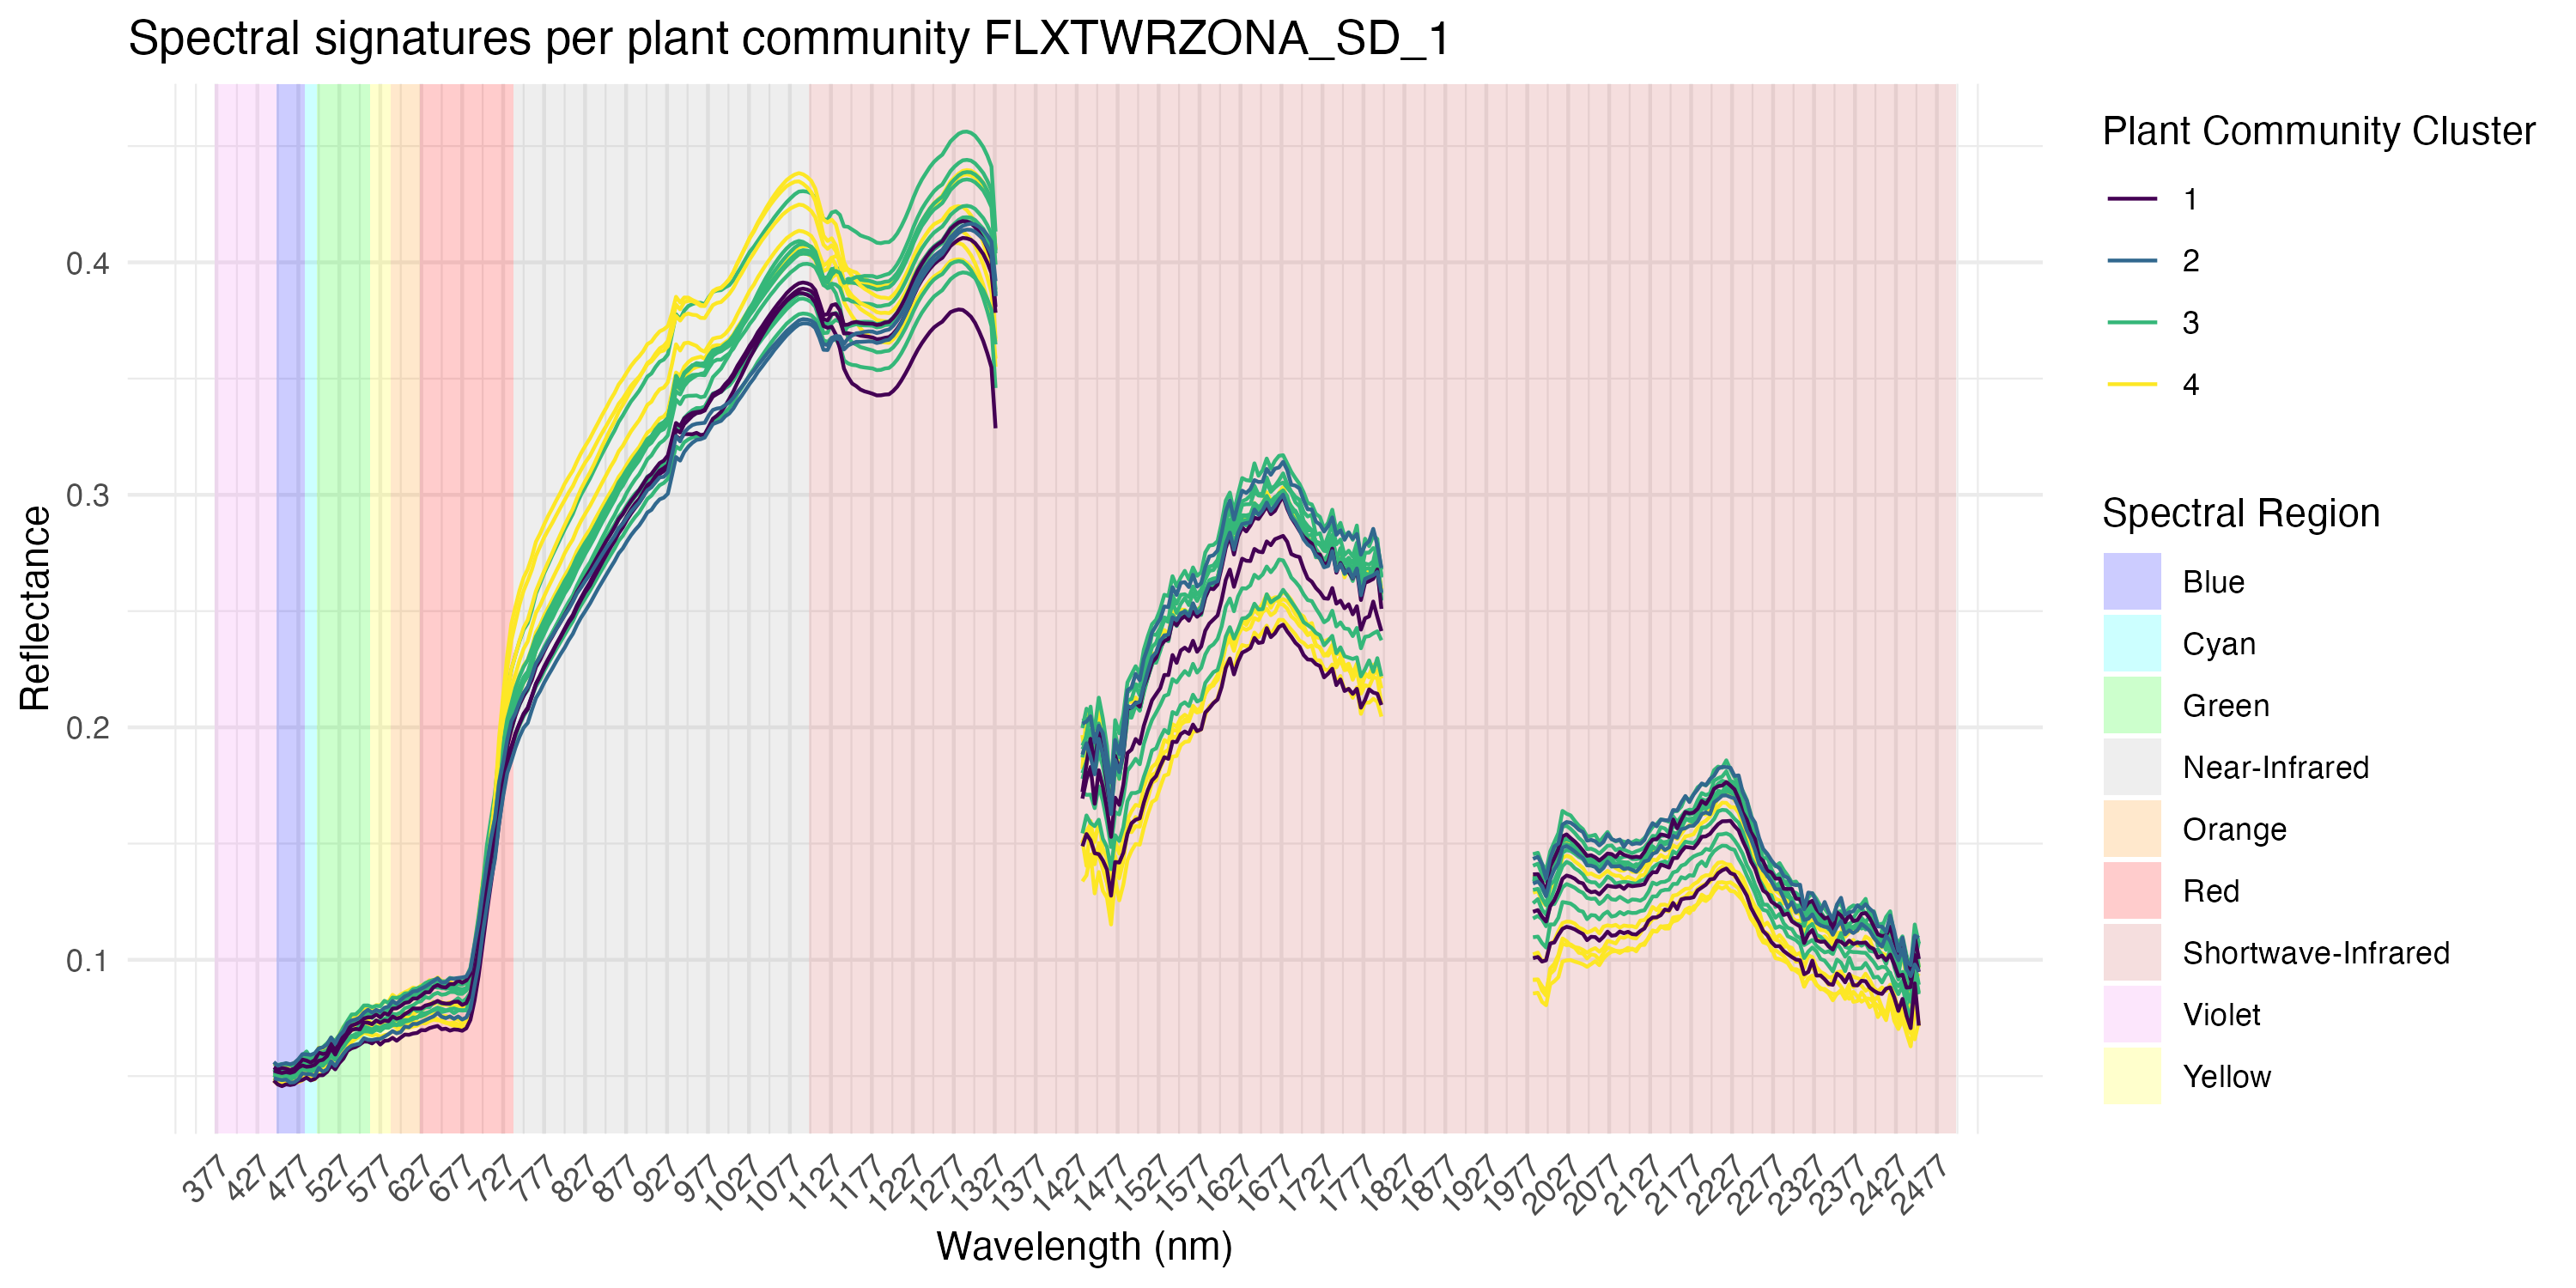
\includegraphics[width=\textwidth]{Figures/spectral_signatures/FLXTWRZONA_SD_1_signature_plot_plant_community.png}
    \caption{}
    \label{fig:ss_pc_flxtwrzonasd1}
  \end{subfigure}
  \hfill
  \begin{subfigure}[b]{0.49\textwidth}
    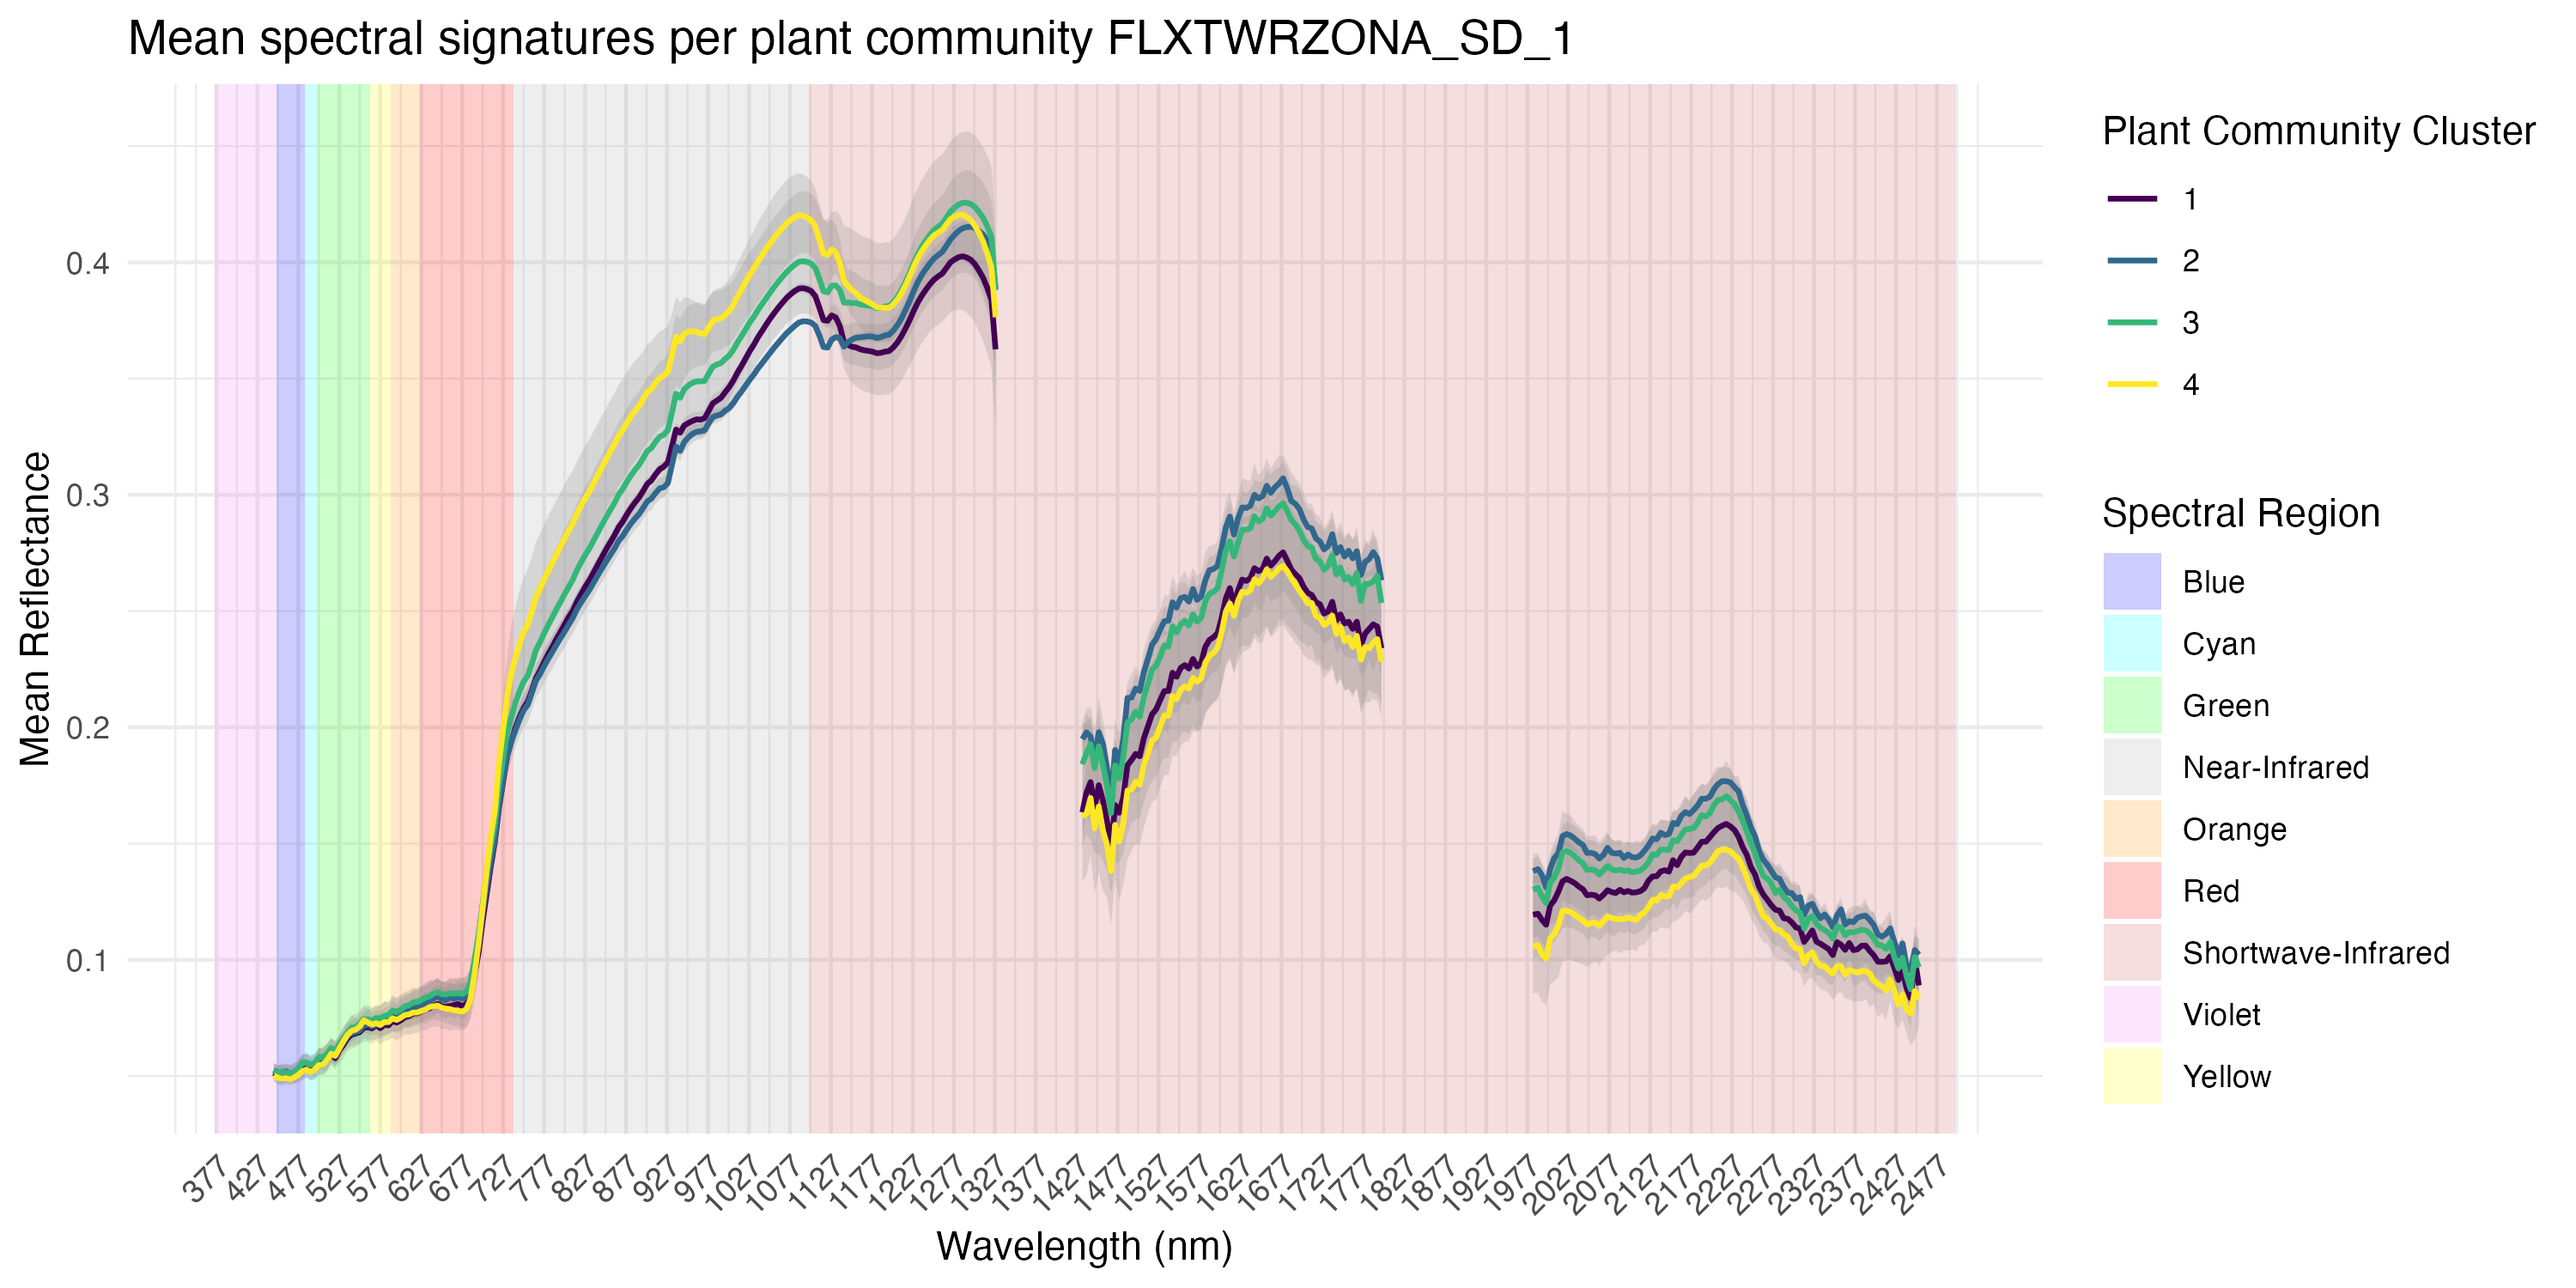
\includegraphics[width=\textwidth]{Figures/spectral_signatures/FLXTWRZONA_SD_1_mean_signature_plot_plant_community.png}
    \caption{}
    \label{fig:mss_pc_flxtwrzonasd1}
  \end{subfigure}

  \caption{Spectral signature plot \ref{fig:ss_pc_flxtwrzonasd1} and mean spectral signature plot \ref{fig:mss_pc_flxtwrzonasd1} grouped by plant community cluster for test site FLXTWRZONA\_SD\_1}
  \label{fig:group_pc_ht_flxtwrzonasd1}
\end{figure}

\subsection{FLXTWRZONA\_SD\_2}

\begin{figure}[H]
  \centering

  \begin{subfigure}[b]{0.49\textwidth}
    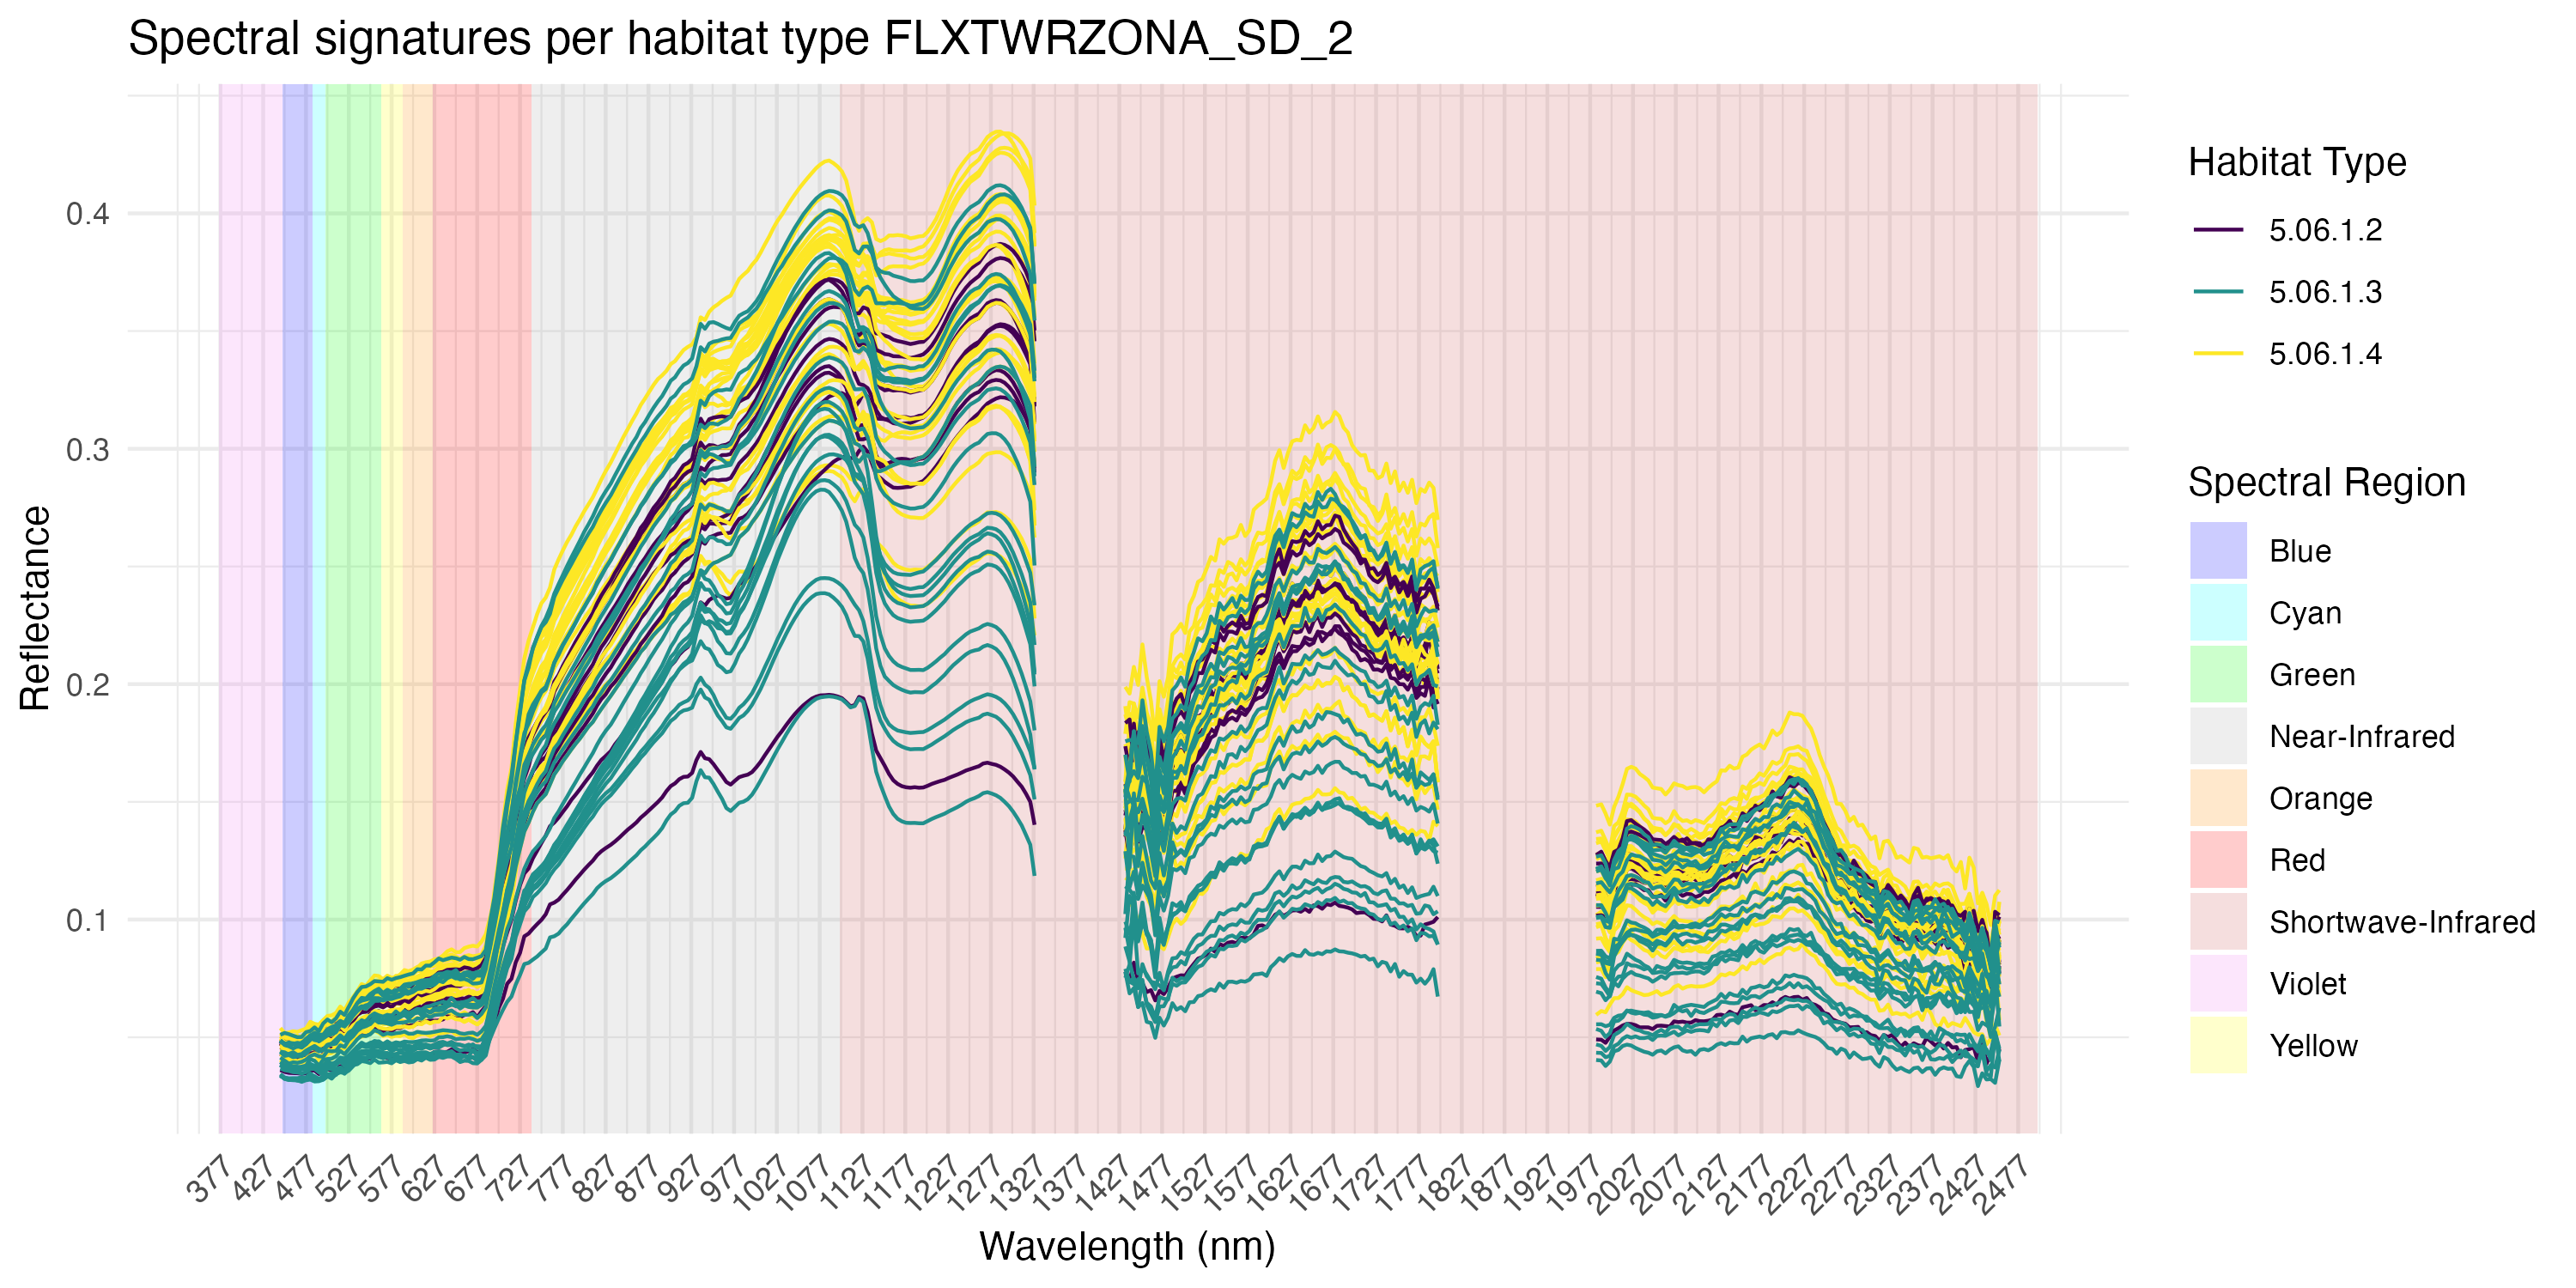
\includegraphics[width=\textwidth]{Figures/spectral_signatures/FLXTWRZONA_SD_2_signature_plot_habitat.png}
    \caption{}
    \label{fig:ss_ht_flxtwrzonasd2}
  \end{subfigure}
  \hfill
  \begin{subfigure}[b]{0.49\textwidth}
    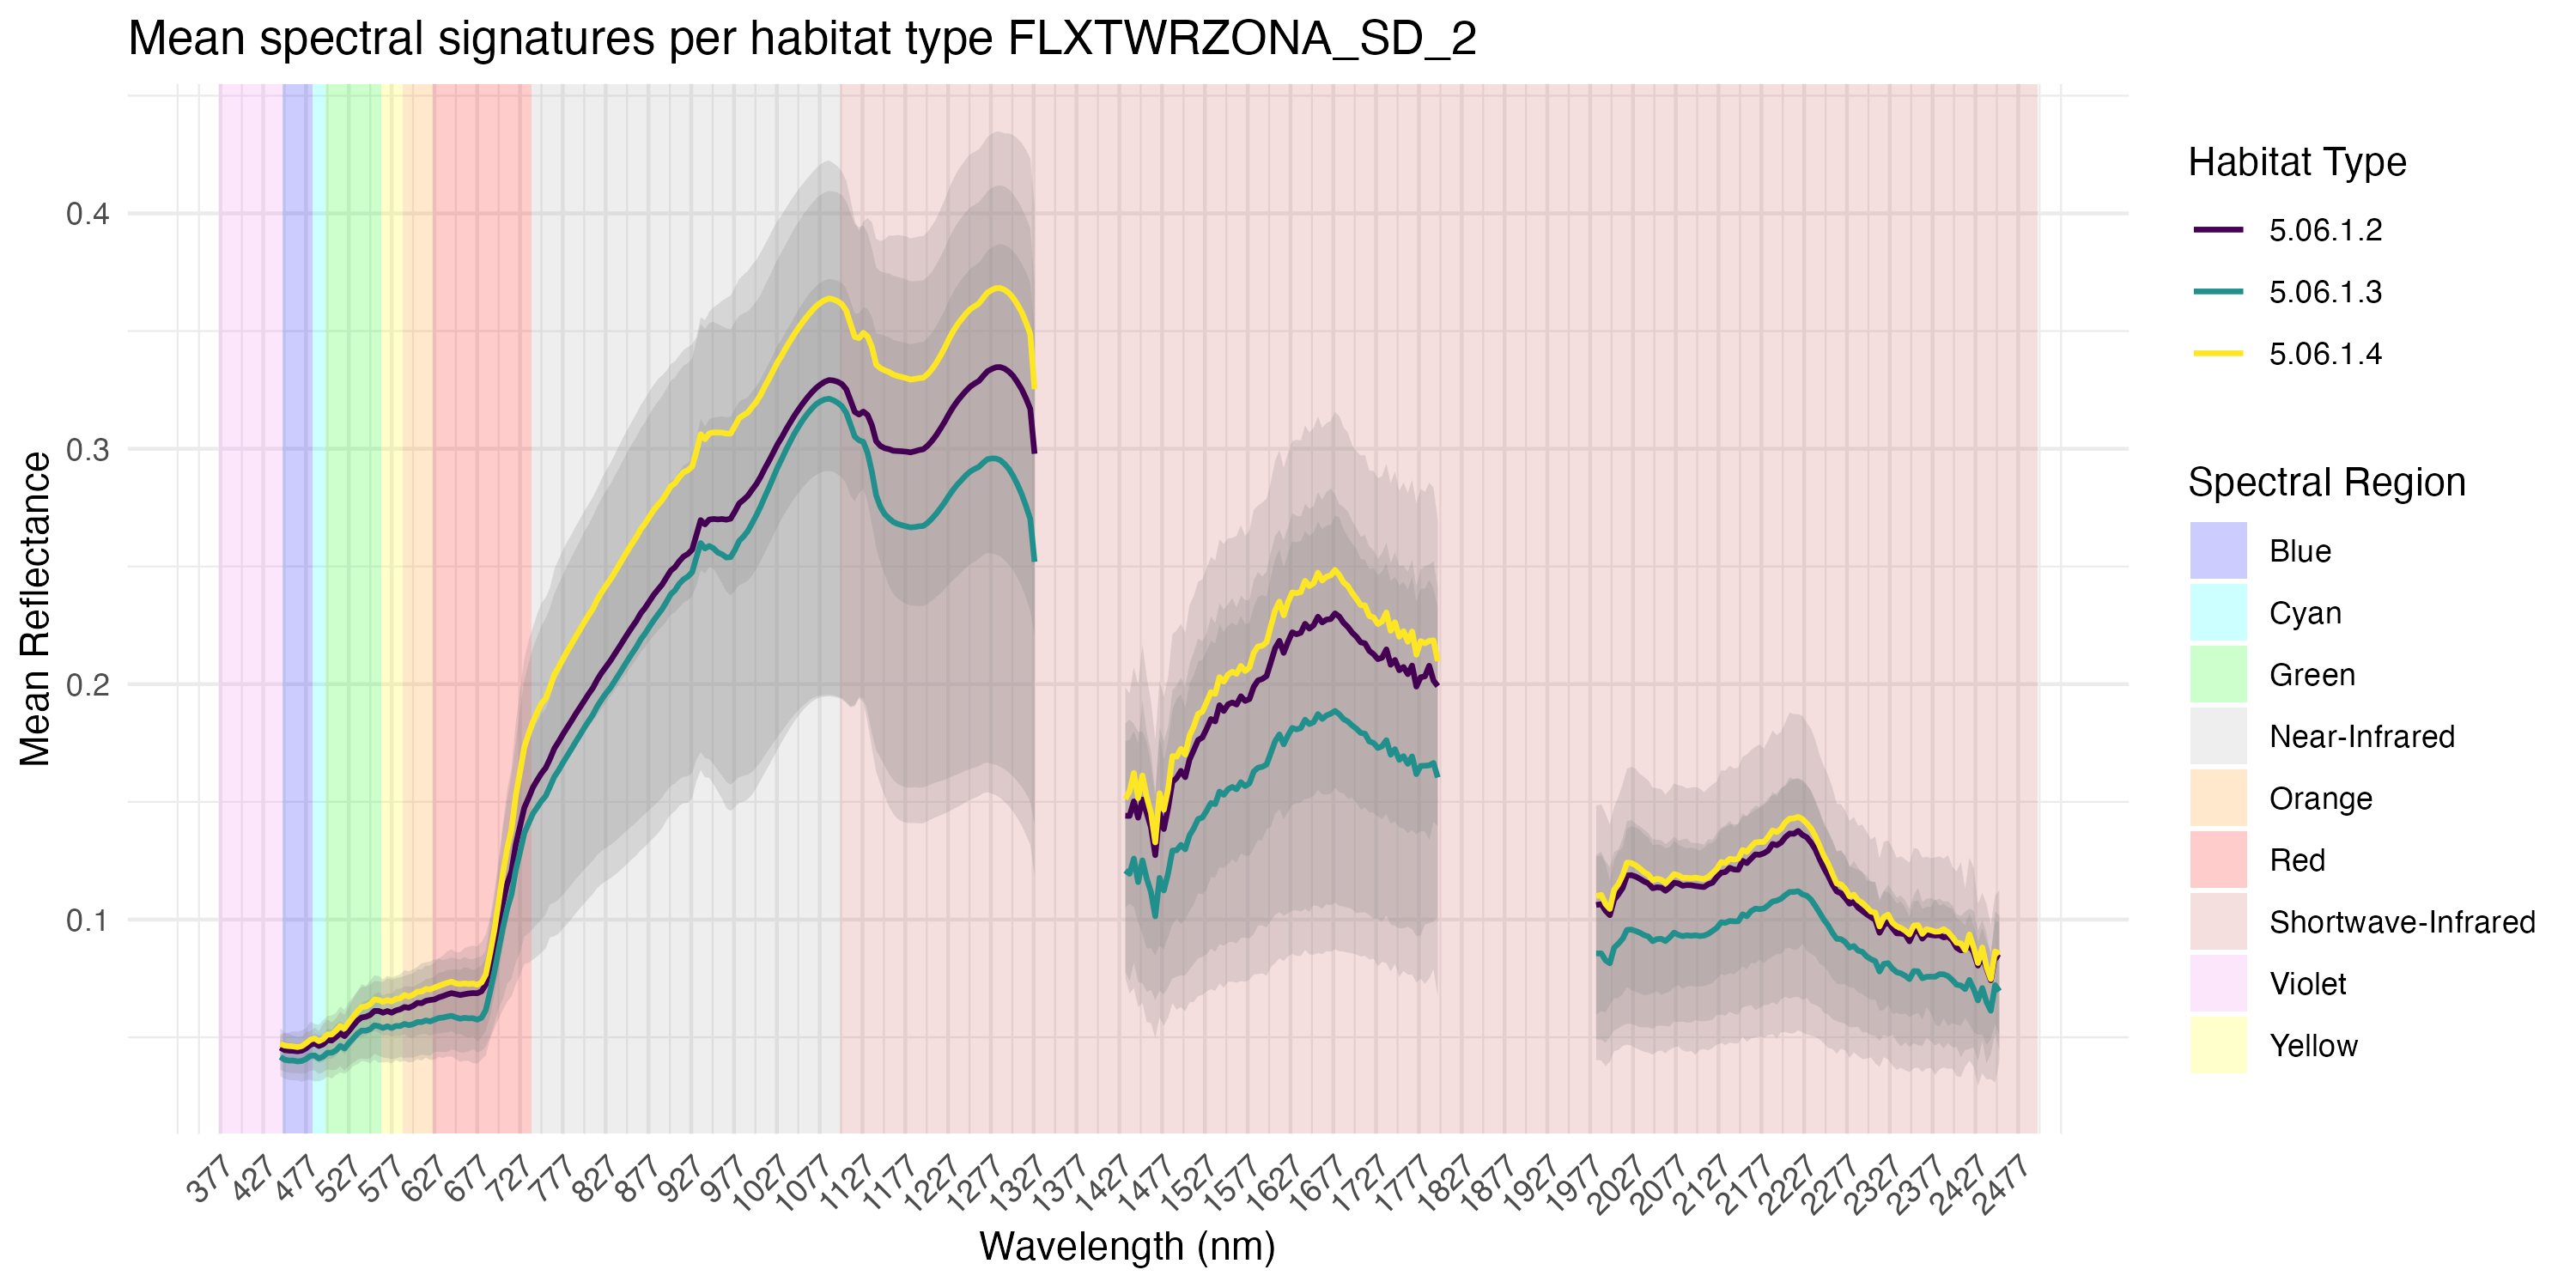
\includegraphics[width=\textwidth]{Figures/spectral_signatures/FLXTWRZONA_SD_2_mean_signature_plot_habitat.png}
    \caption{}
    \label{fig:mss_ht_flxtwrzonasd2}
  \end{subfigure}

  \caption{Spectral signature plot \ref{fig:ss_ht_flxtwrzonasd2} and mean spectral signature plot \ref{fig:mss_ht_flxtwrzonasd2} grouped by habitat type for test site FLXTWRZONA\_SD\_2}
  \label{fig:group_ss_ht_flxtwrzonasd2}
\end{figure}

\begin{figure}[H]
  \centering

  \begin{subfigure}[b]{0.49\textwidth}
    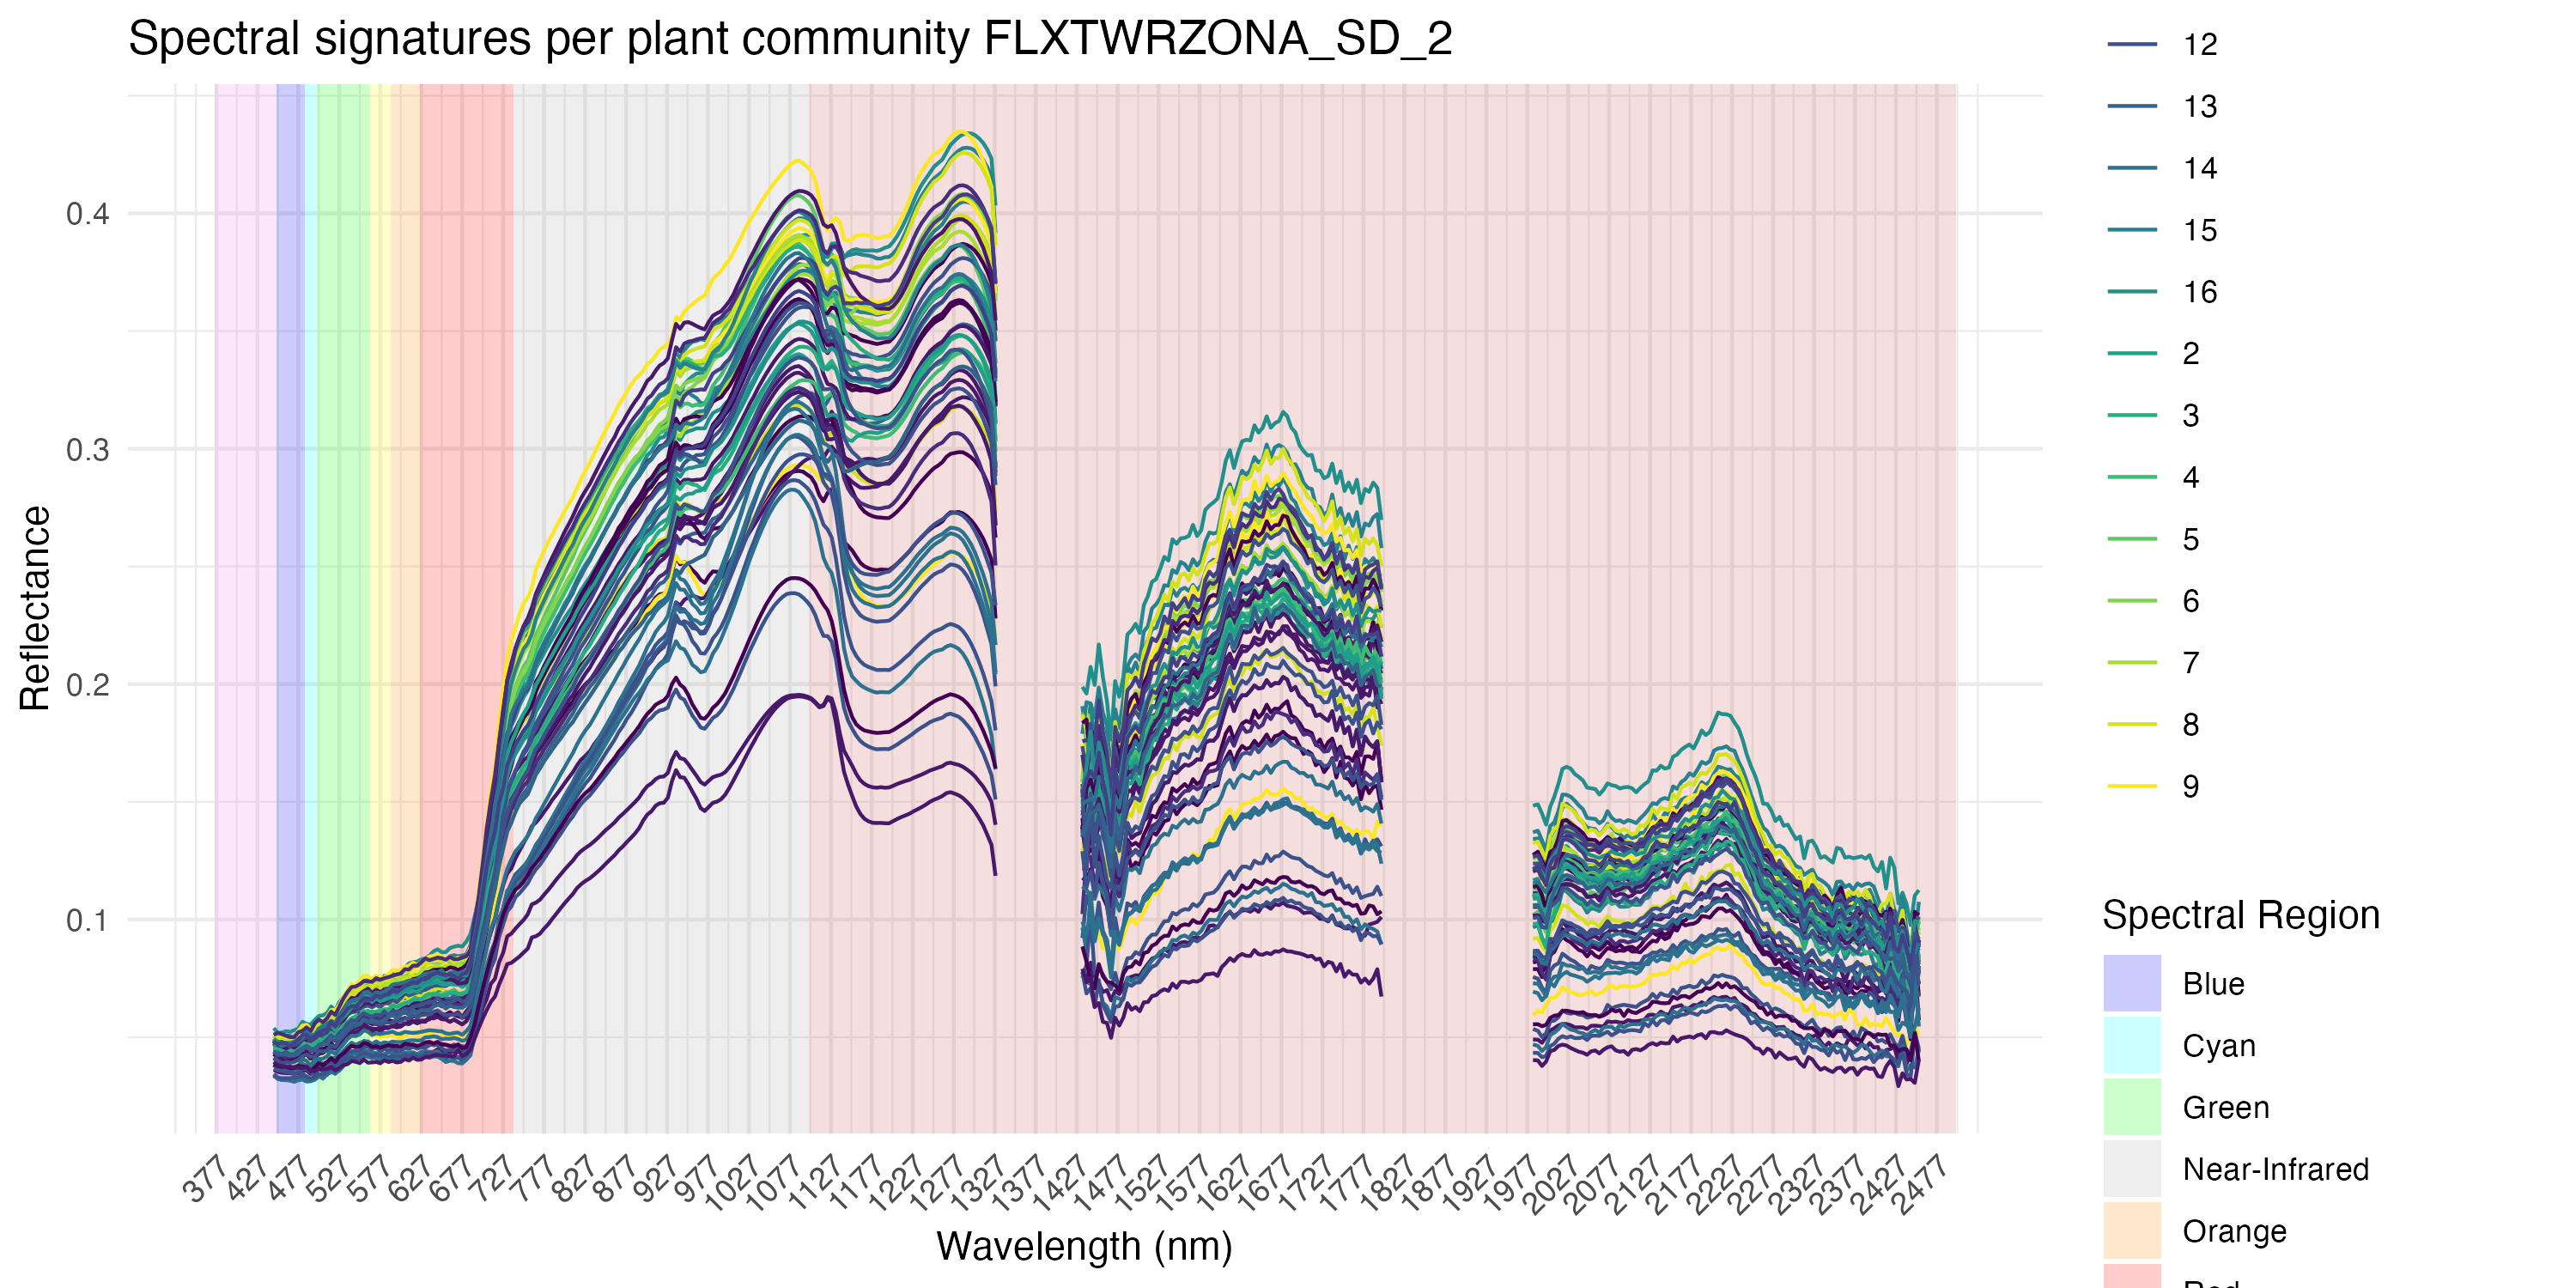
\includegraphics[width=\textwidth]{Figures/spectral_signatures/FLXTWRZONA_SD_2_signature_plot_plant_community.png}
    \caption{}
    \label{fig:ss_pc_flxtwrzonasd2}
  \end{subfigure}
  \hfill
  \begin{subfigure}[b]{0.49\textwidth}
    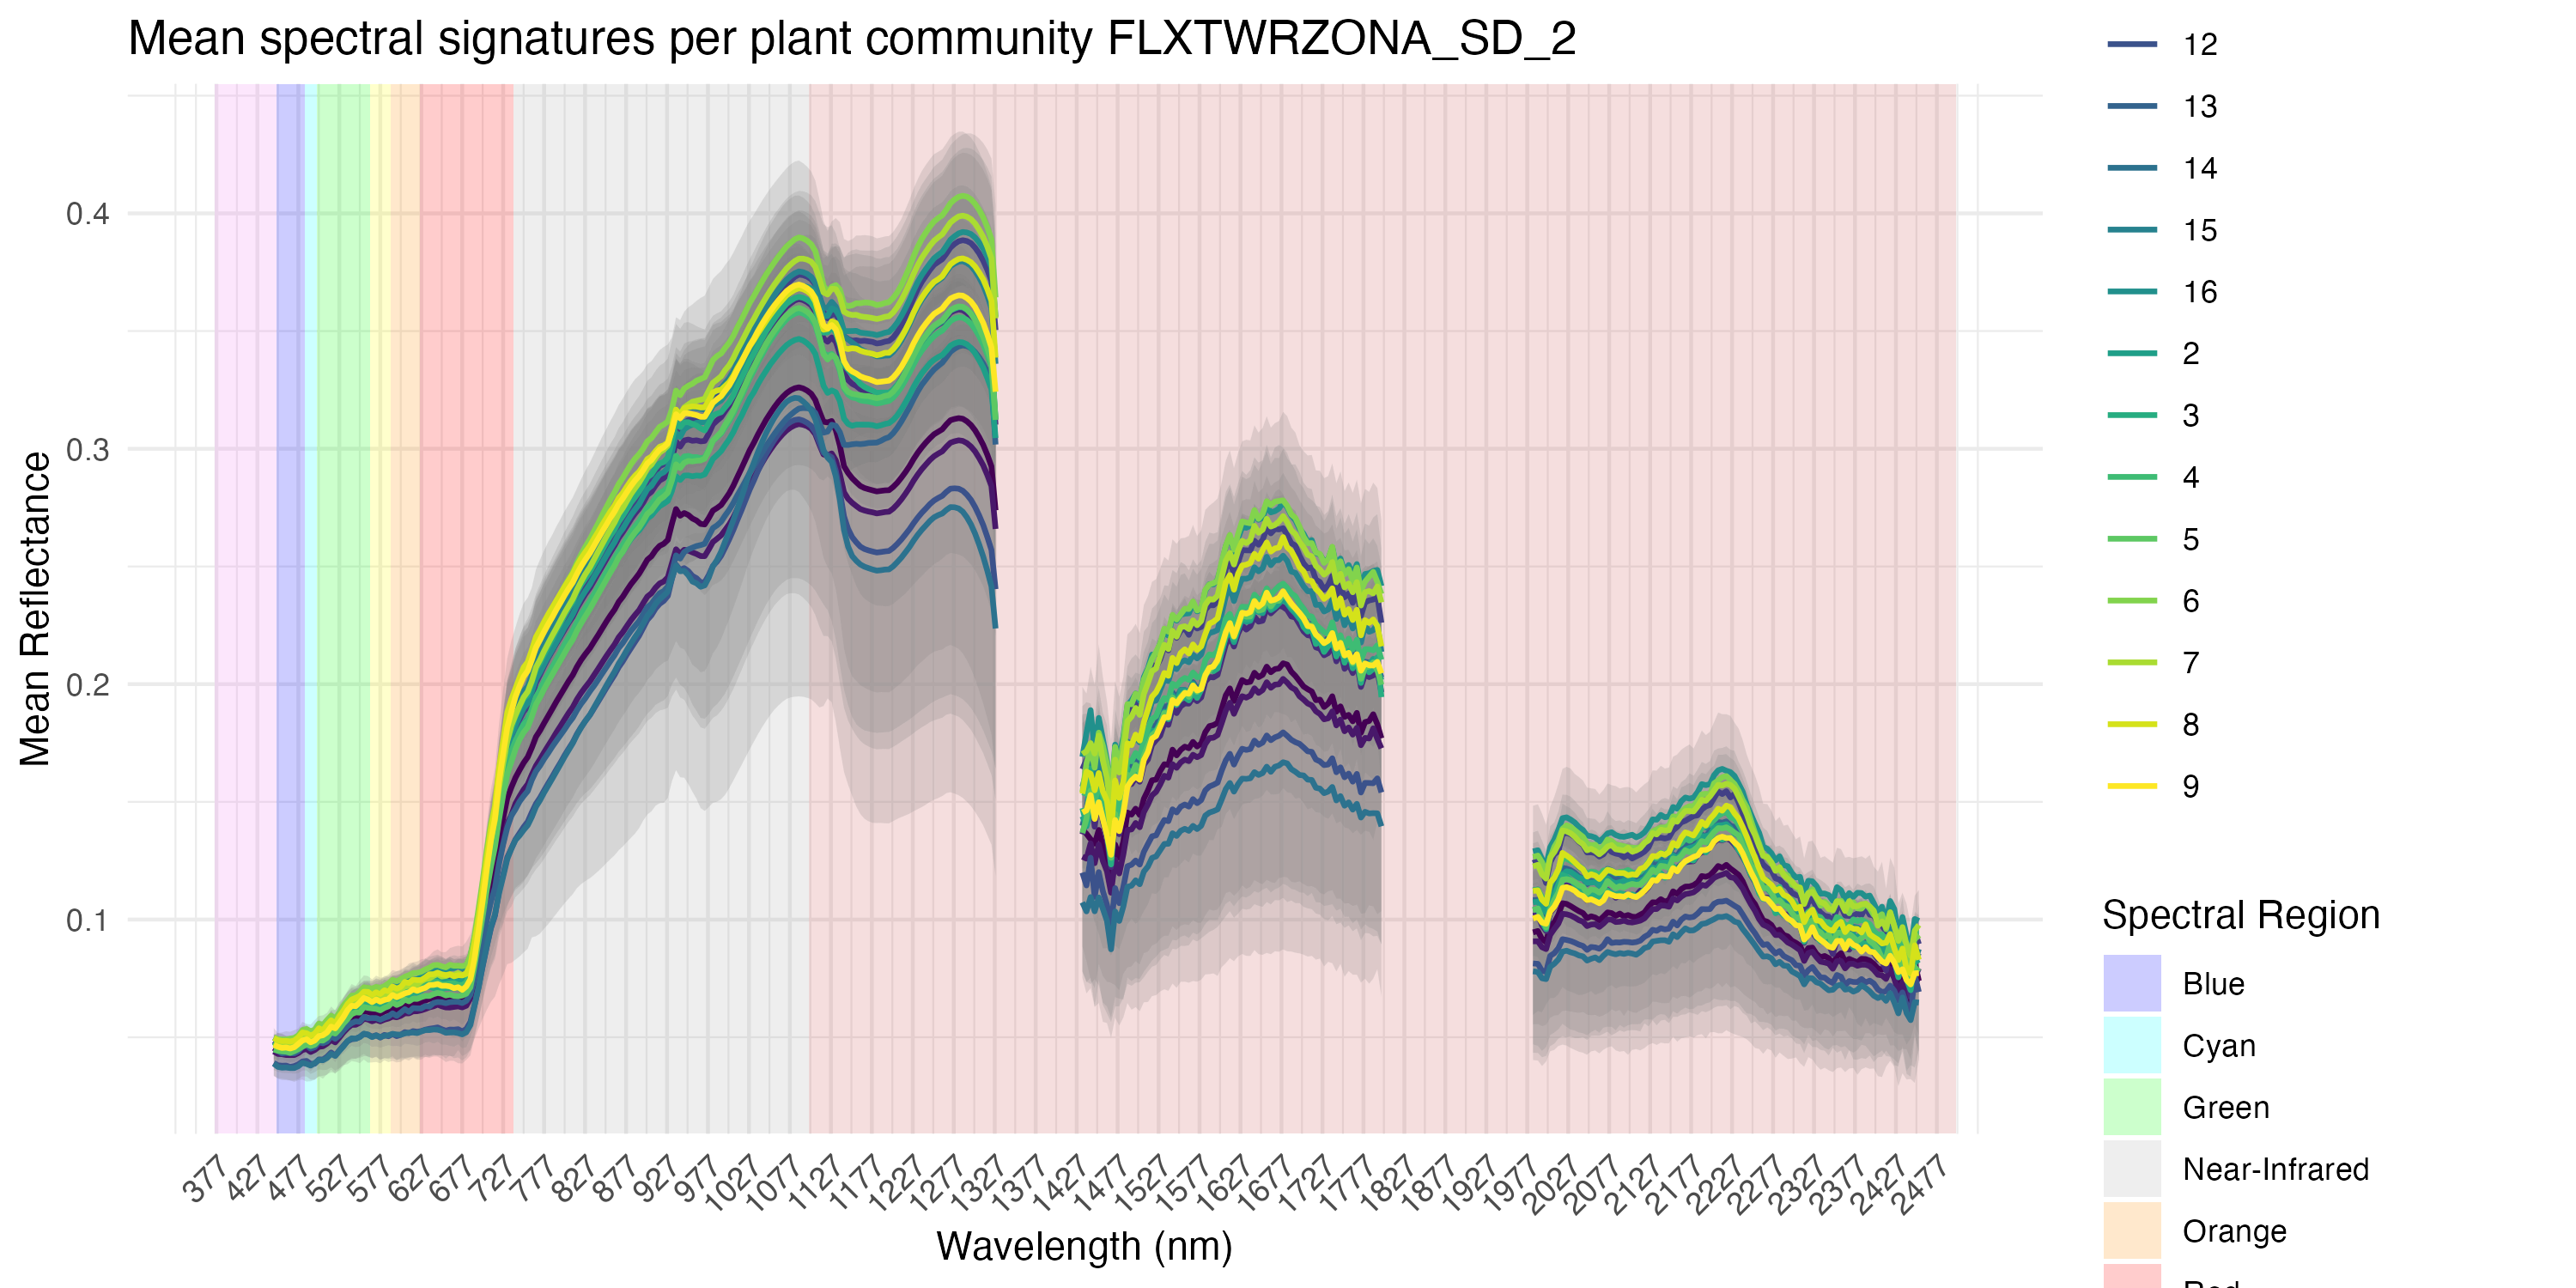
\includegraphics[width=\textwidth]{Figures/spectral_signatures/FLXTWRZONA_SD_2_mean_signature_plot_plant_community.png}
    \caption{}
    \label{fig:mss_pc_flxtwrzonasd2}
  \end{subfigure}

  \caption{Spectral signature plot \ref{fig:ss_pc_flxtwrzonasd2} and mean spectral signature plot \ref{fig:mss_pc_flxtwrzonasd2} grouped by plant community cluster for test site FLXTWRZONA\_SD\_2}
  \label{fig:group_pc_ht_flxtwrzonasd2}
\end{figure}

\subsection{FLXTWRZONA\_SD\_3}

\begin{figure}[H]
  \centering

  \begin{subfigure}[b]{0.49\textwidth}
    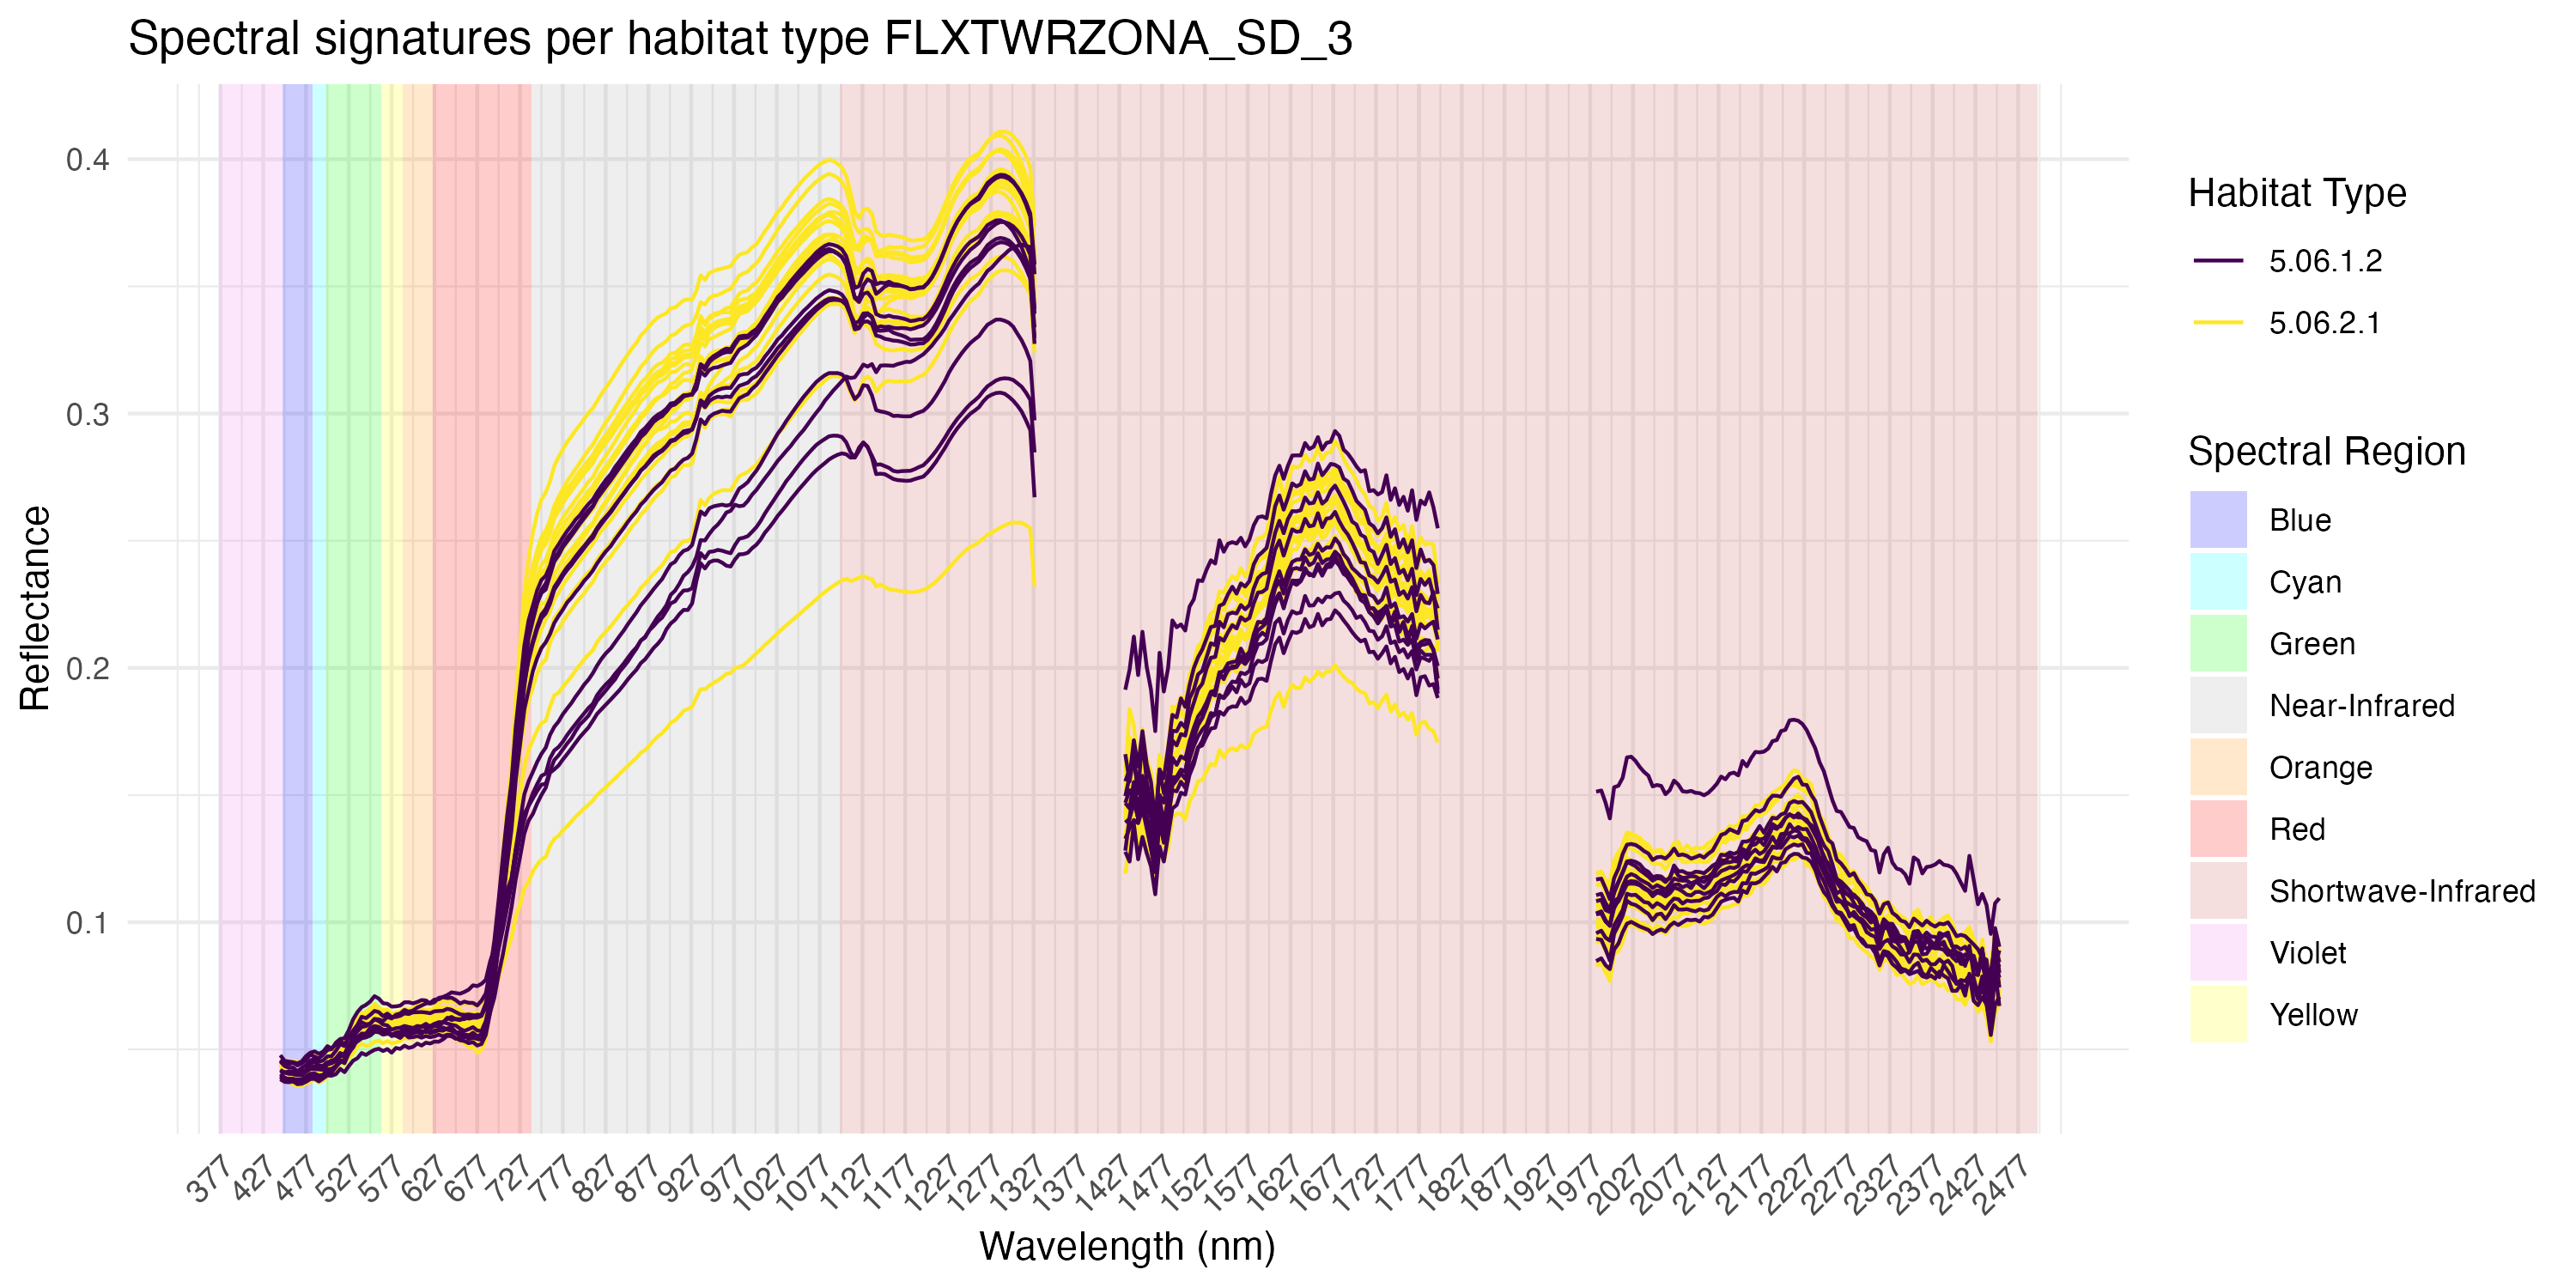
\includegraphics[width=\textwidth]{Figures/spectral_signatures/FLXTWRZONA_SD_3_signature_plot_habitat.png}
    \caption{}
    \label{fig:ss_ht_flxtwrzonasd3}
  \end{subfigure}
  \hfill
  \begin{subfigure}[b]{0.49\textwidth}
    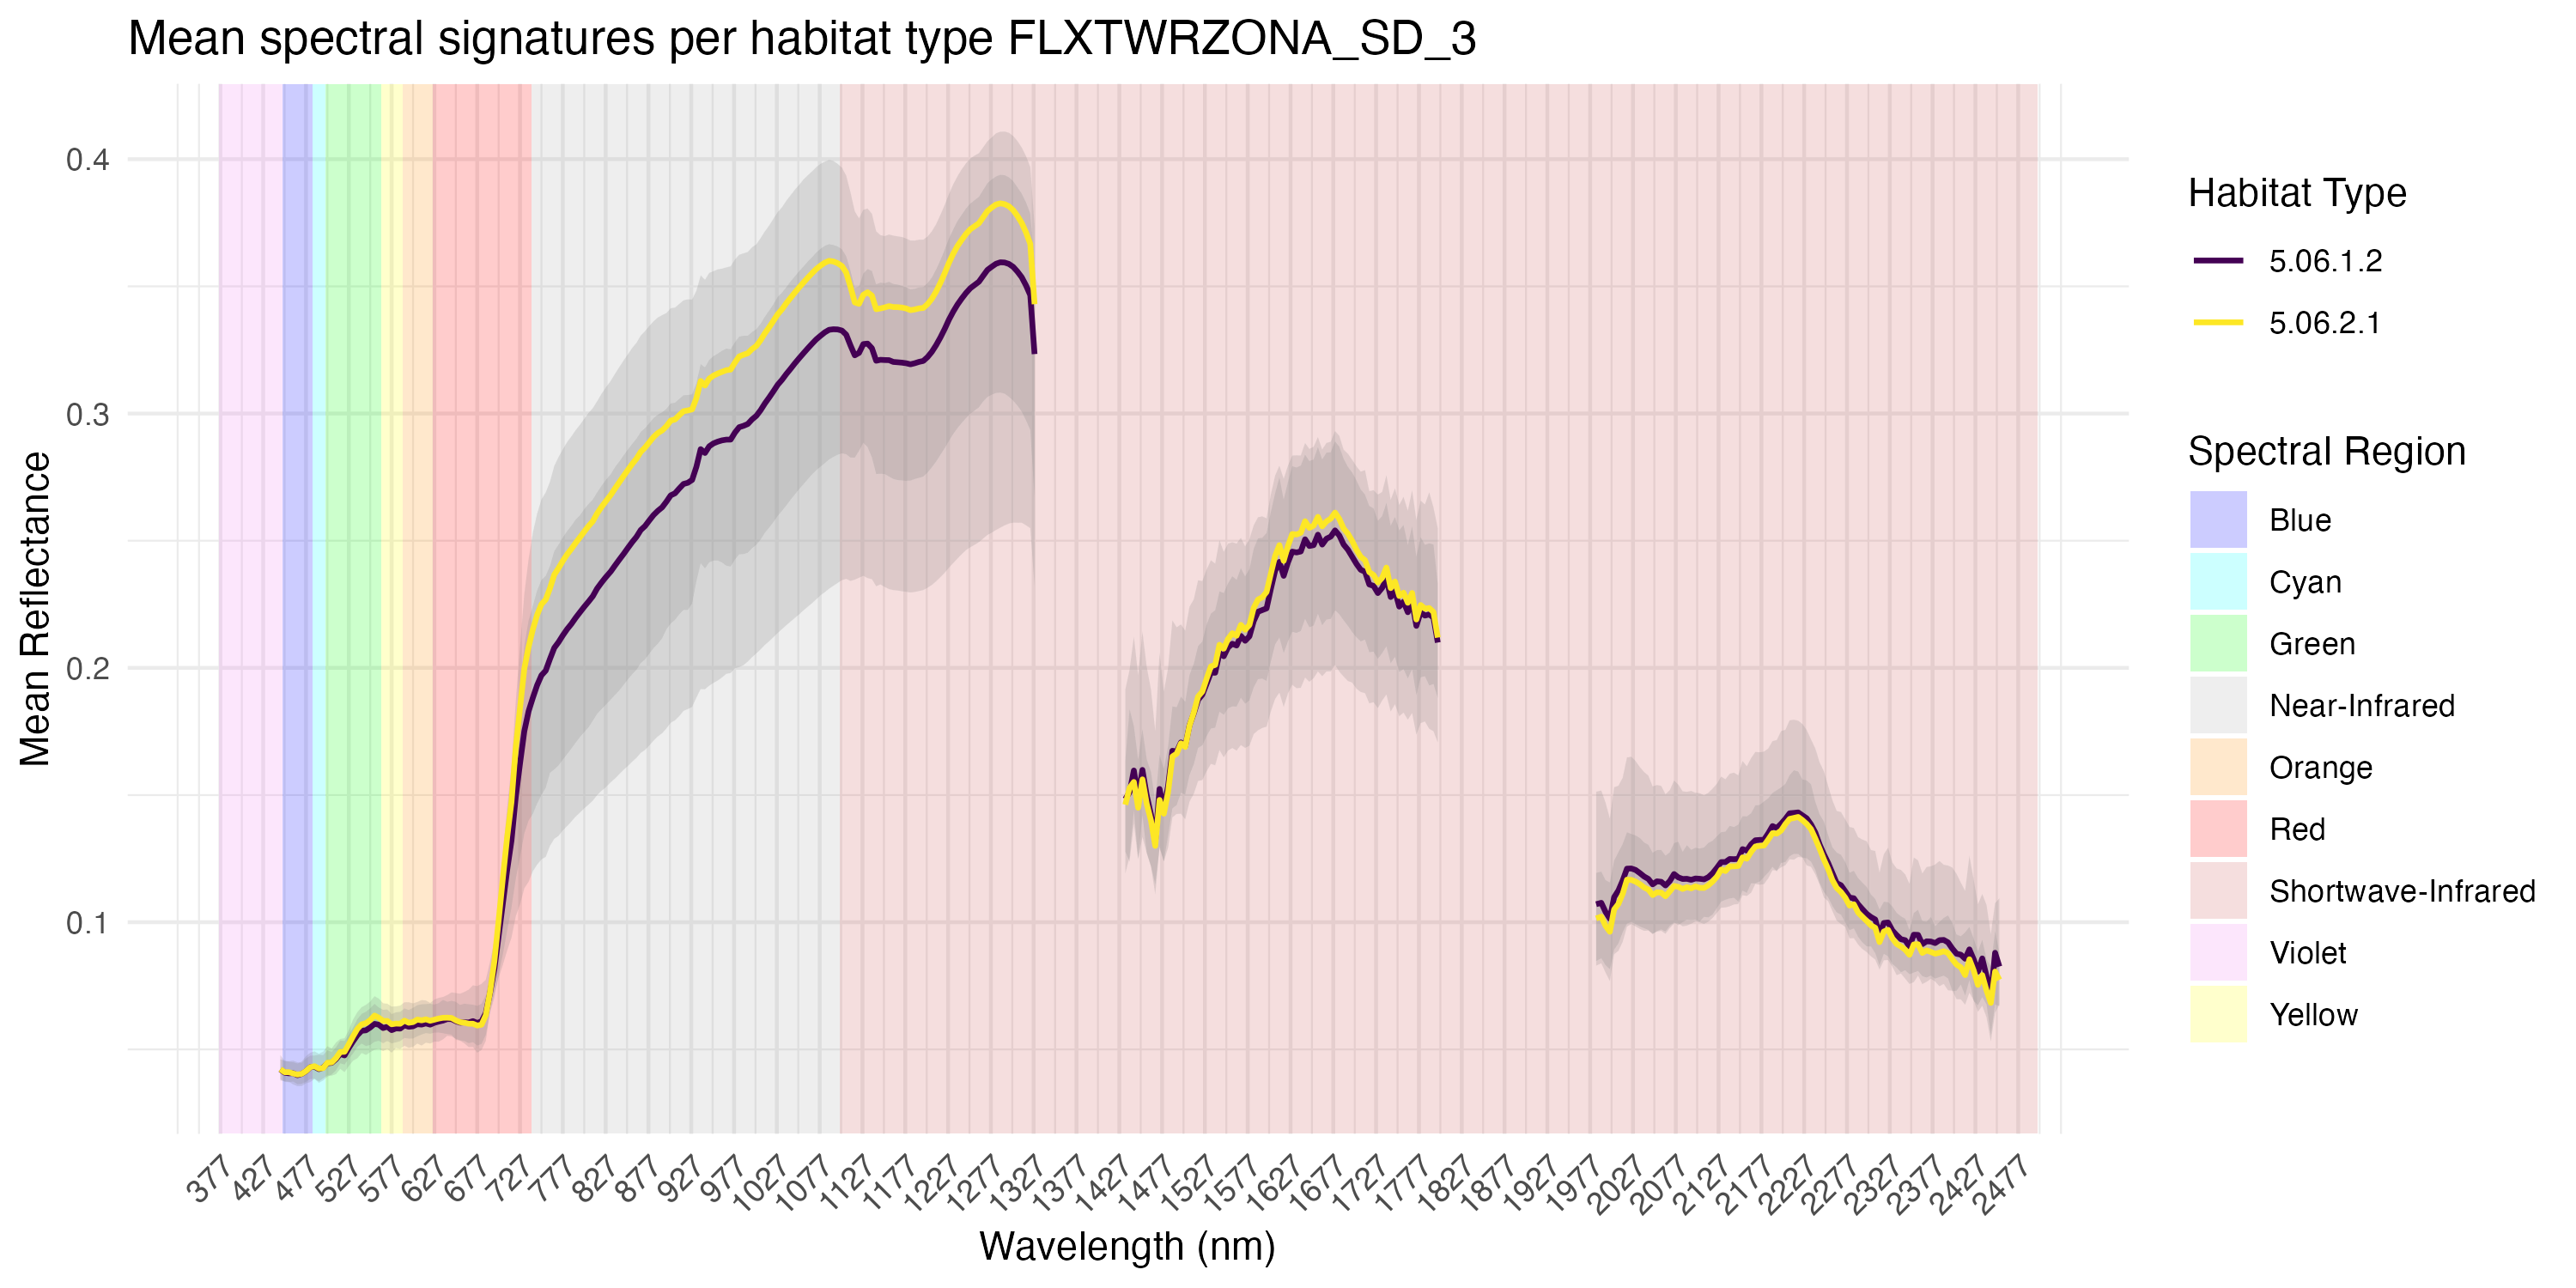
\includegraphics[width=\textwidth]{Figures/spectral_signatures/FLXTWRZONA_SD_3_mean_signature_plot_habitat.png}
    \caption{}
    \label{fig:mss_ht_flxtwrzonasd3}
  \end{subfigure}

  \caption{Spectral signature plot \ref{fig:ss_ht_flxtwrzonasd3} and mean spectral signature plot \ref{fig:mss_ht_flxtwrzonasd3} grouped by habitat type for test site FLXTWRZONA\_SD\_3}
  \label{fig:group_ss_ht_flxtwrzonasd3}
\end{figure}

\begin{figure}[H]
  \centering

  \begin{subfigure}[b]{0.49\textwidth}
    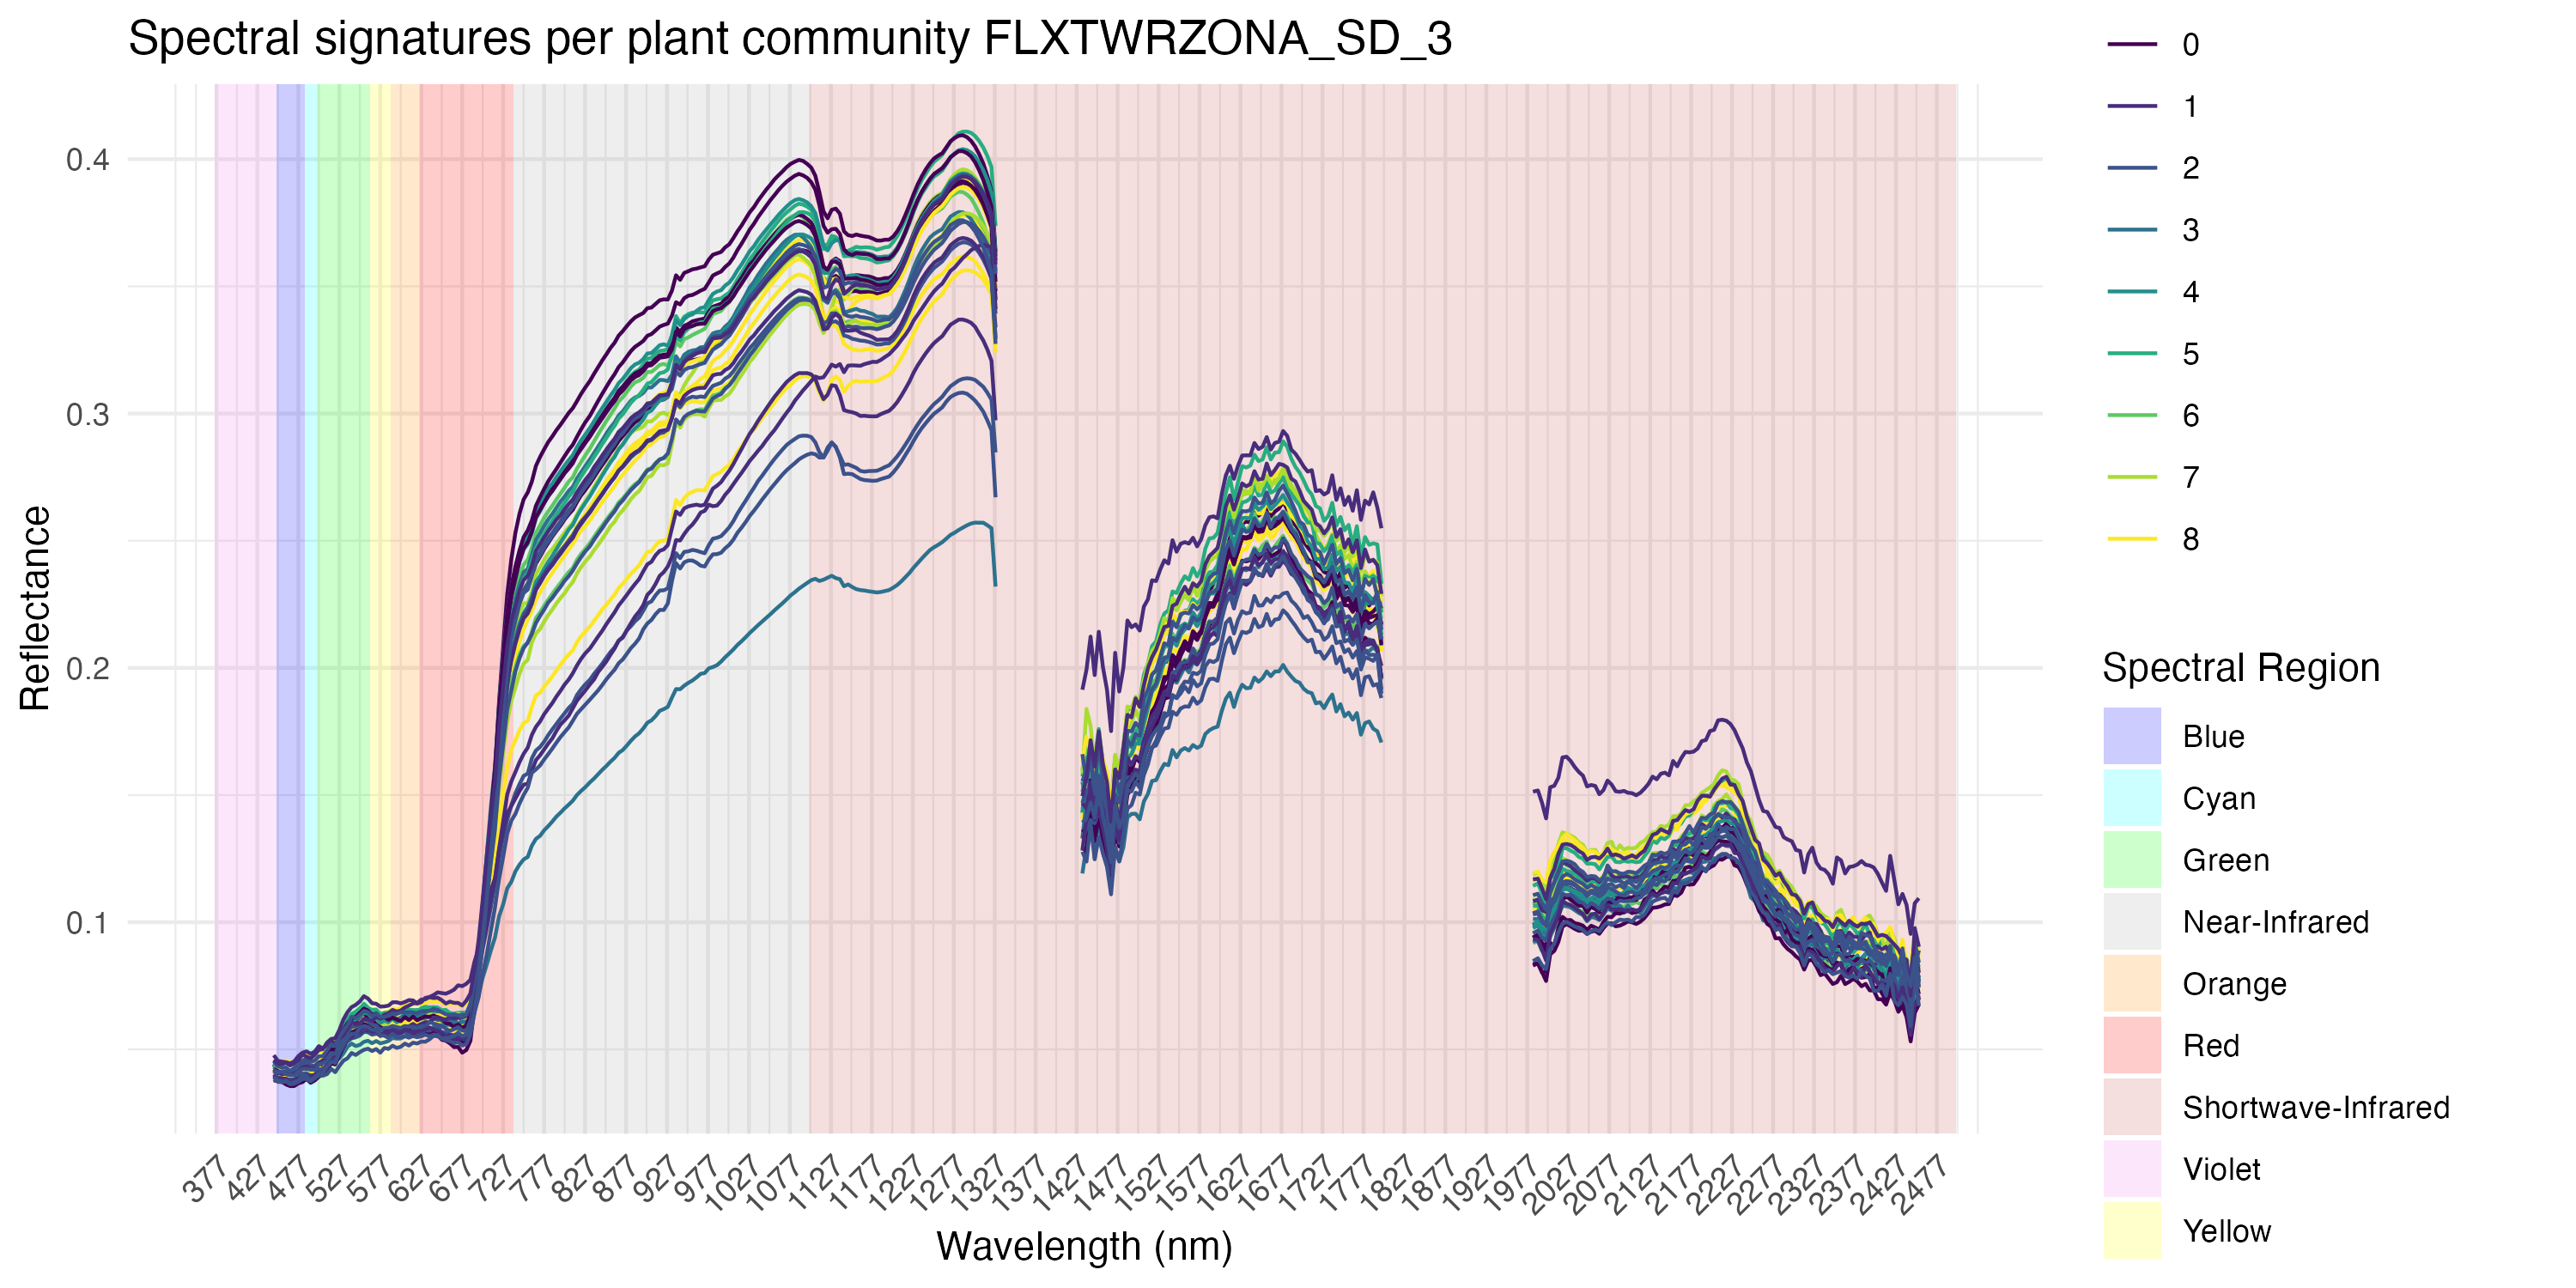
\includegraphics[width=\textwidth]{Figures/spectral_signatures/FLXTWRZONA_SD_3_signature_plot_plant_community.png}
    \caption{}
    \label{fig:ss_pc_flxtwrzonasd3}
  \end{subfigure}
  \hfill
  \begin{subfigure}[b]{0.49\textwidth}
    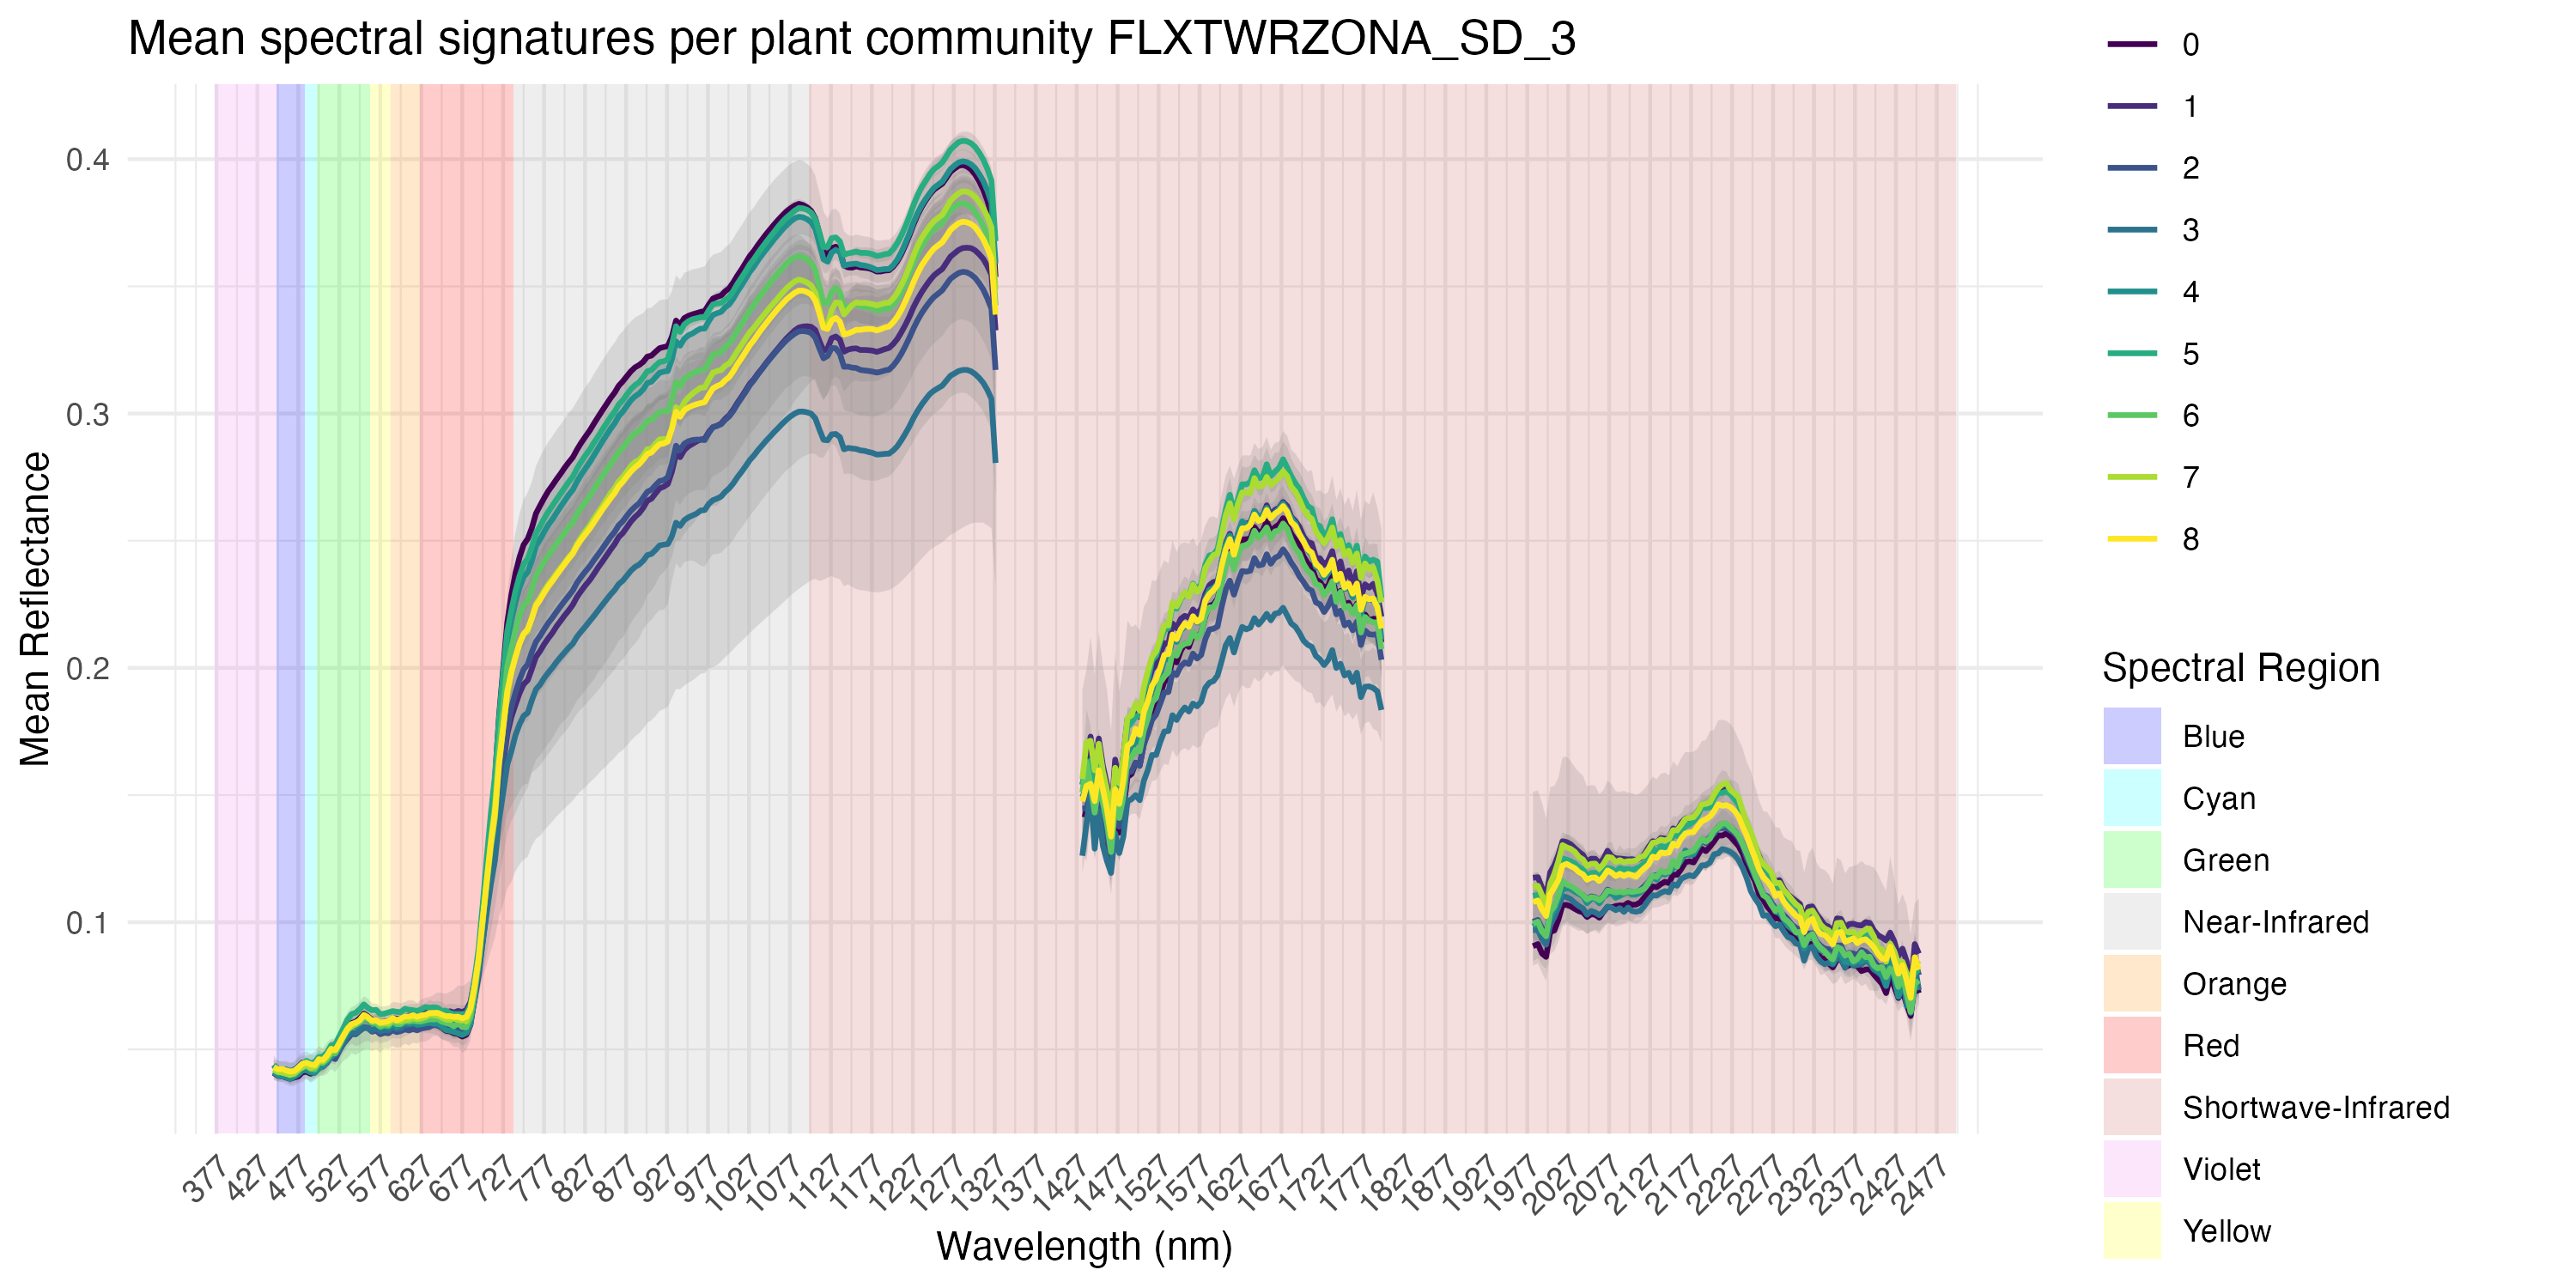
\includegraphics[width=\textwidth]{Figures/spectral_signatures/FLXTWRZONA_SD_3_mean_signature_plot_plant_community.png}
    \caption{}
    \label{fig:mss_pc_flxtwrzonasd3}
  \end{subfigure}

  \caption{Spectral signature plot \ref{fig:ss_pc_flxtwrzonasd3} and mean spectral signature plot \ref{fig:mss_pc_flxtwrzonasd3} grouped by plant community cluster for test site FLXTWRZONA\_SD\_3}
  \label{fig:group_pc_ht_flxtwrzonasd3}
\end{figure}

\subsection{FLXTWRZONA\_SD\_4}

\begin{figure}[H]
  \centering

  \begin{subfigure}[b]{0.49\textwidth}
    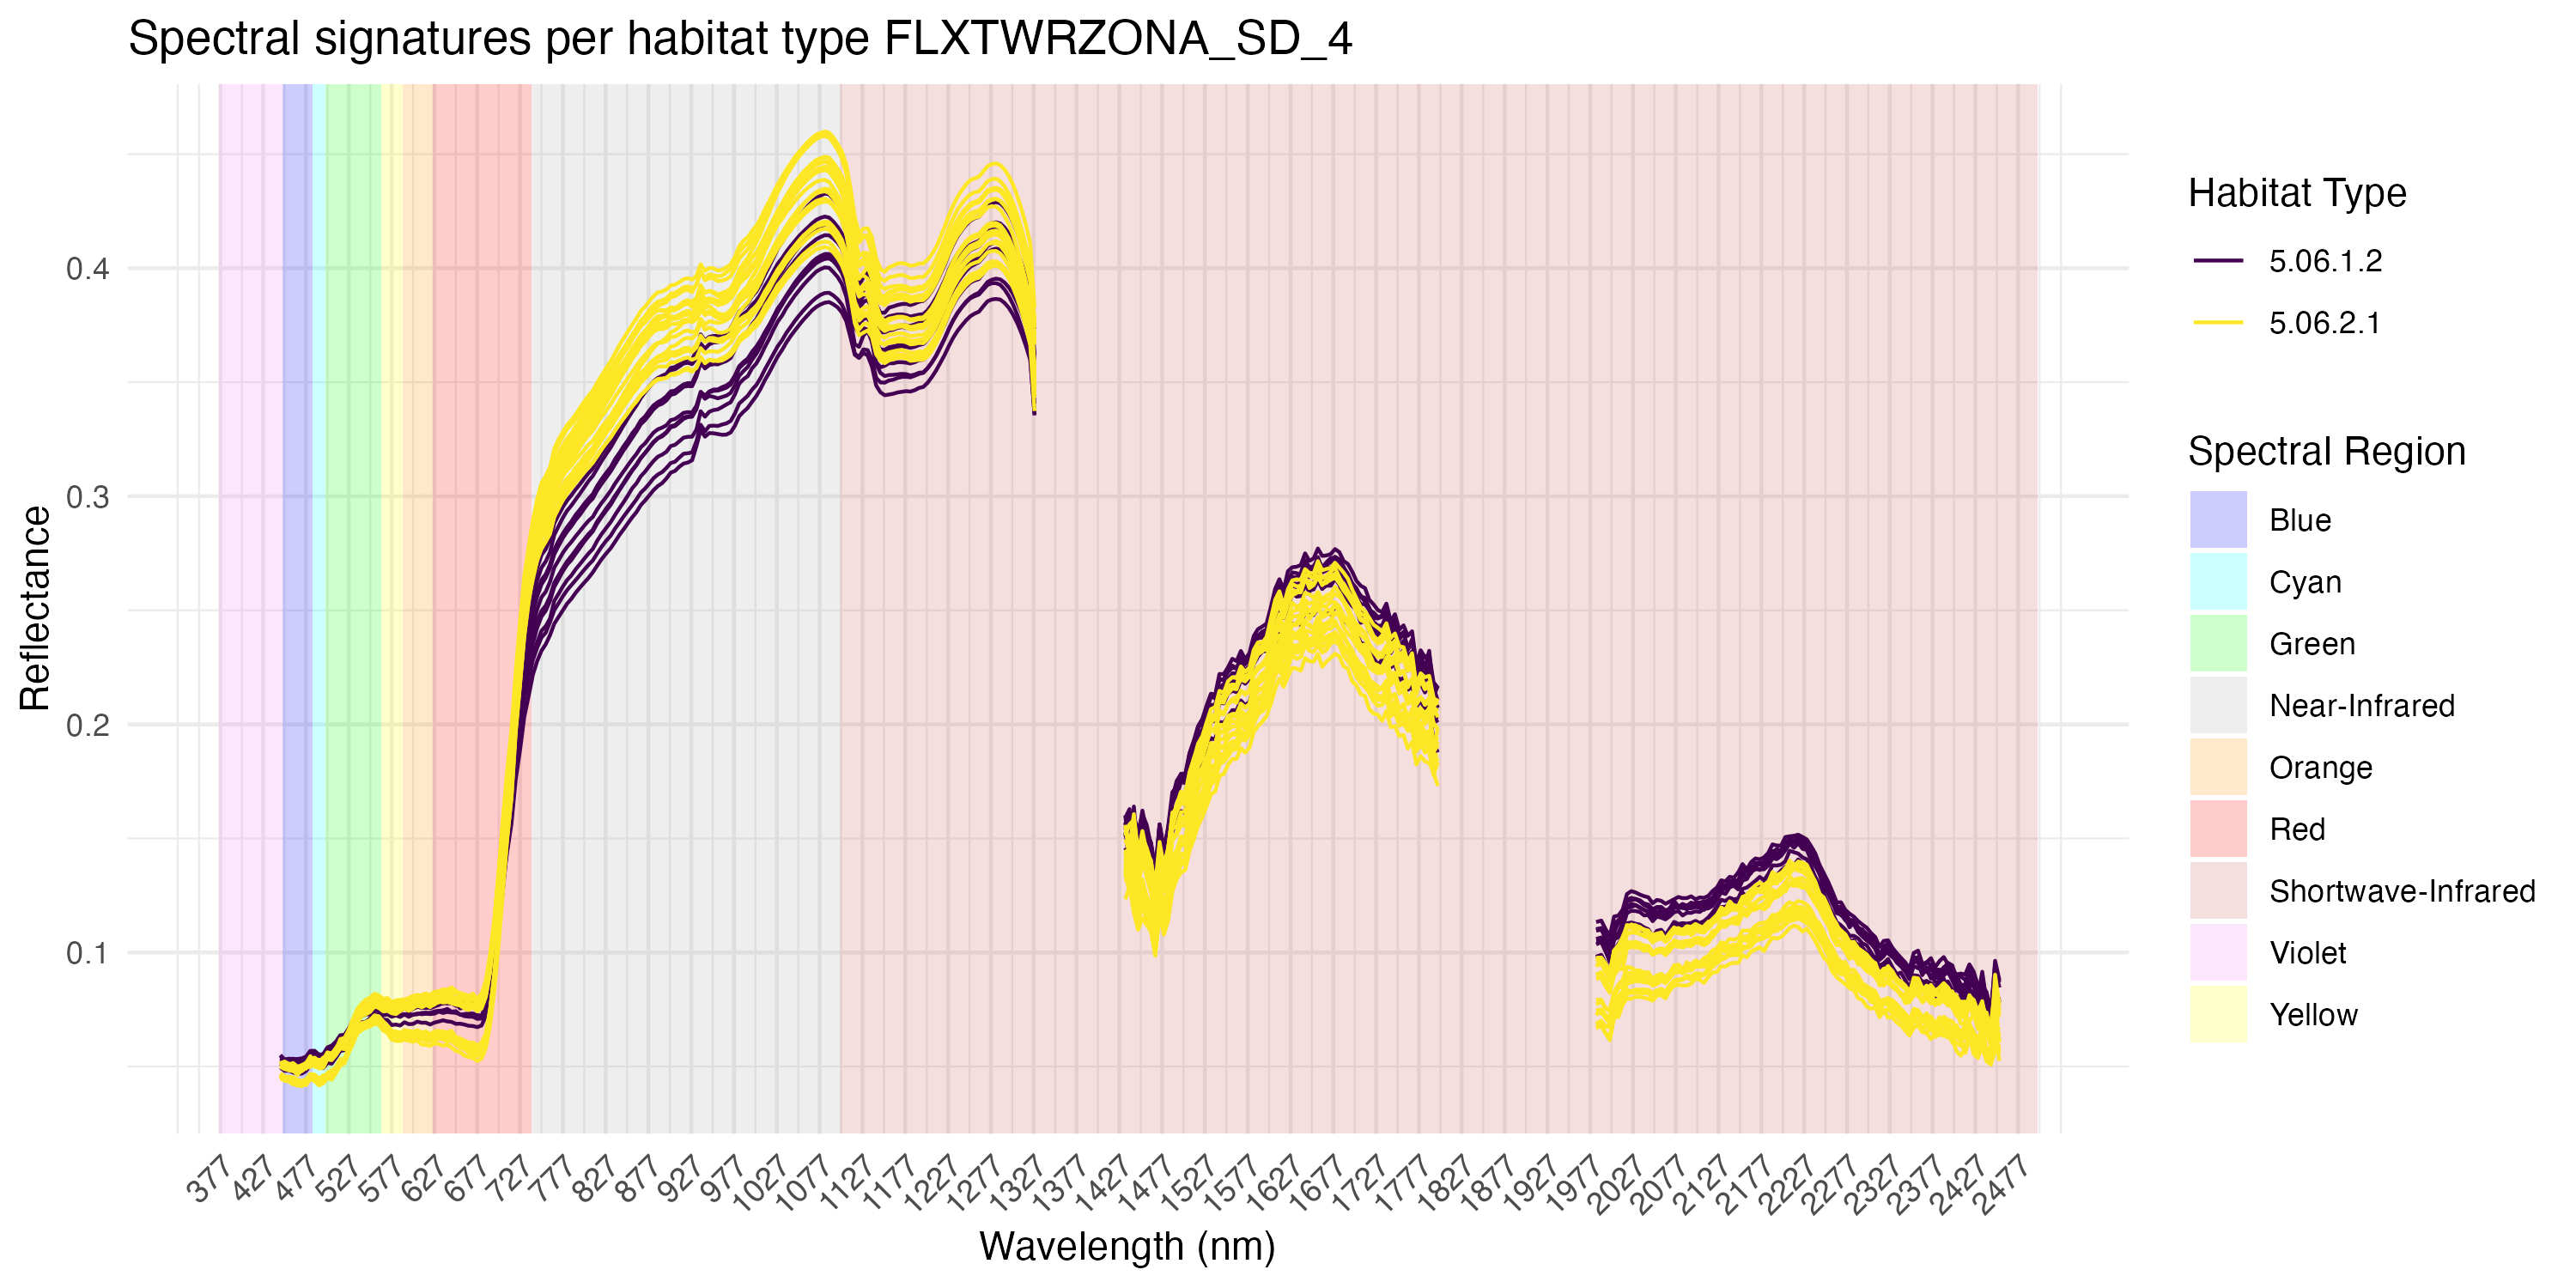
\includegraphics[width=\textwidth]{Figures/spectral_signatures/FLXTWRZONA_SD_4_signature_plot_habitat.png}
    \caption{}
    \label{fig:ss_ht_flxtwrzonasd4}
  \end{subfigure}
  \hfill
  \begin{subfigure}[b]{0.49\textwidth}
    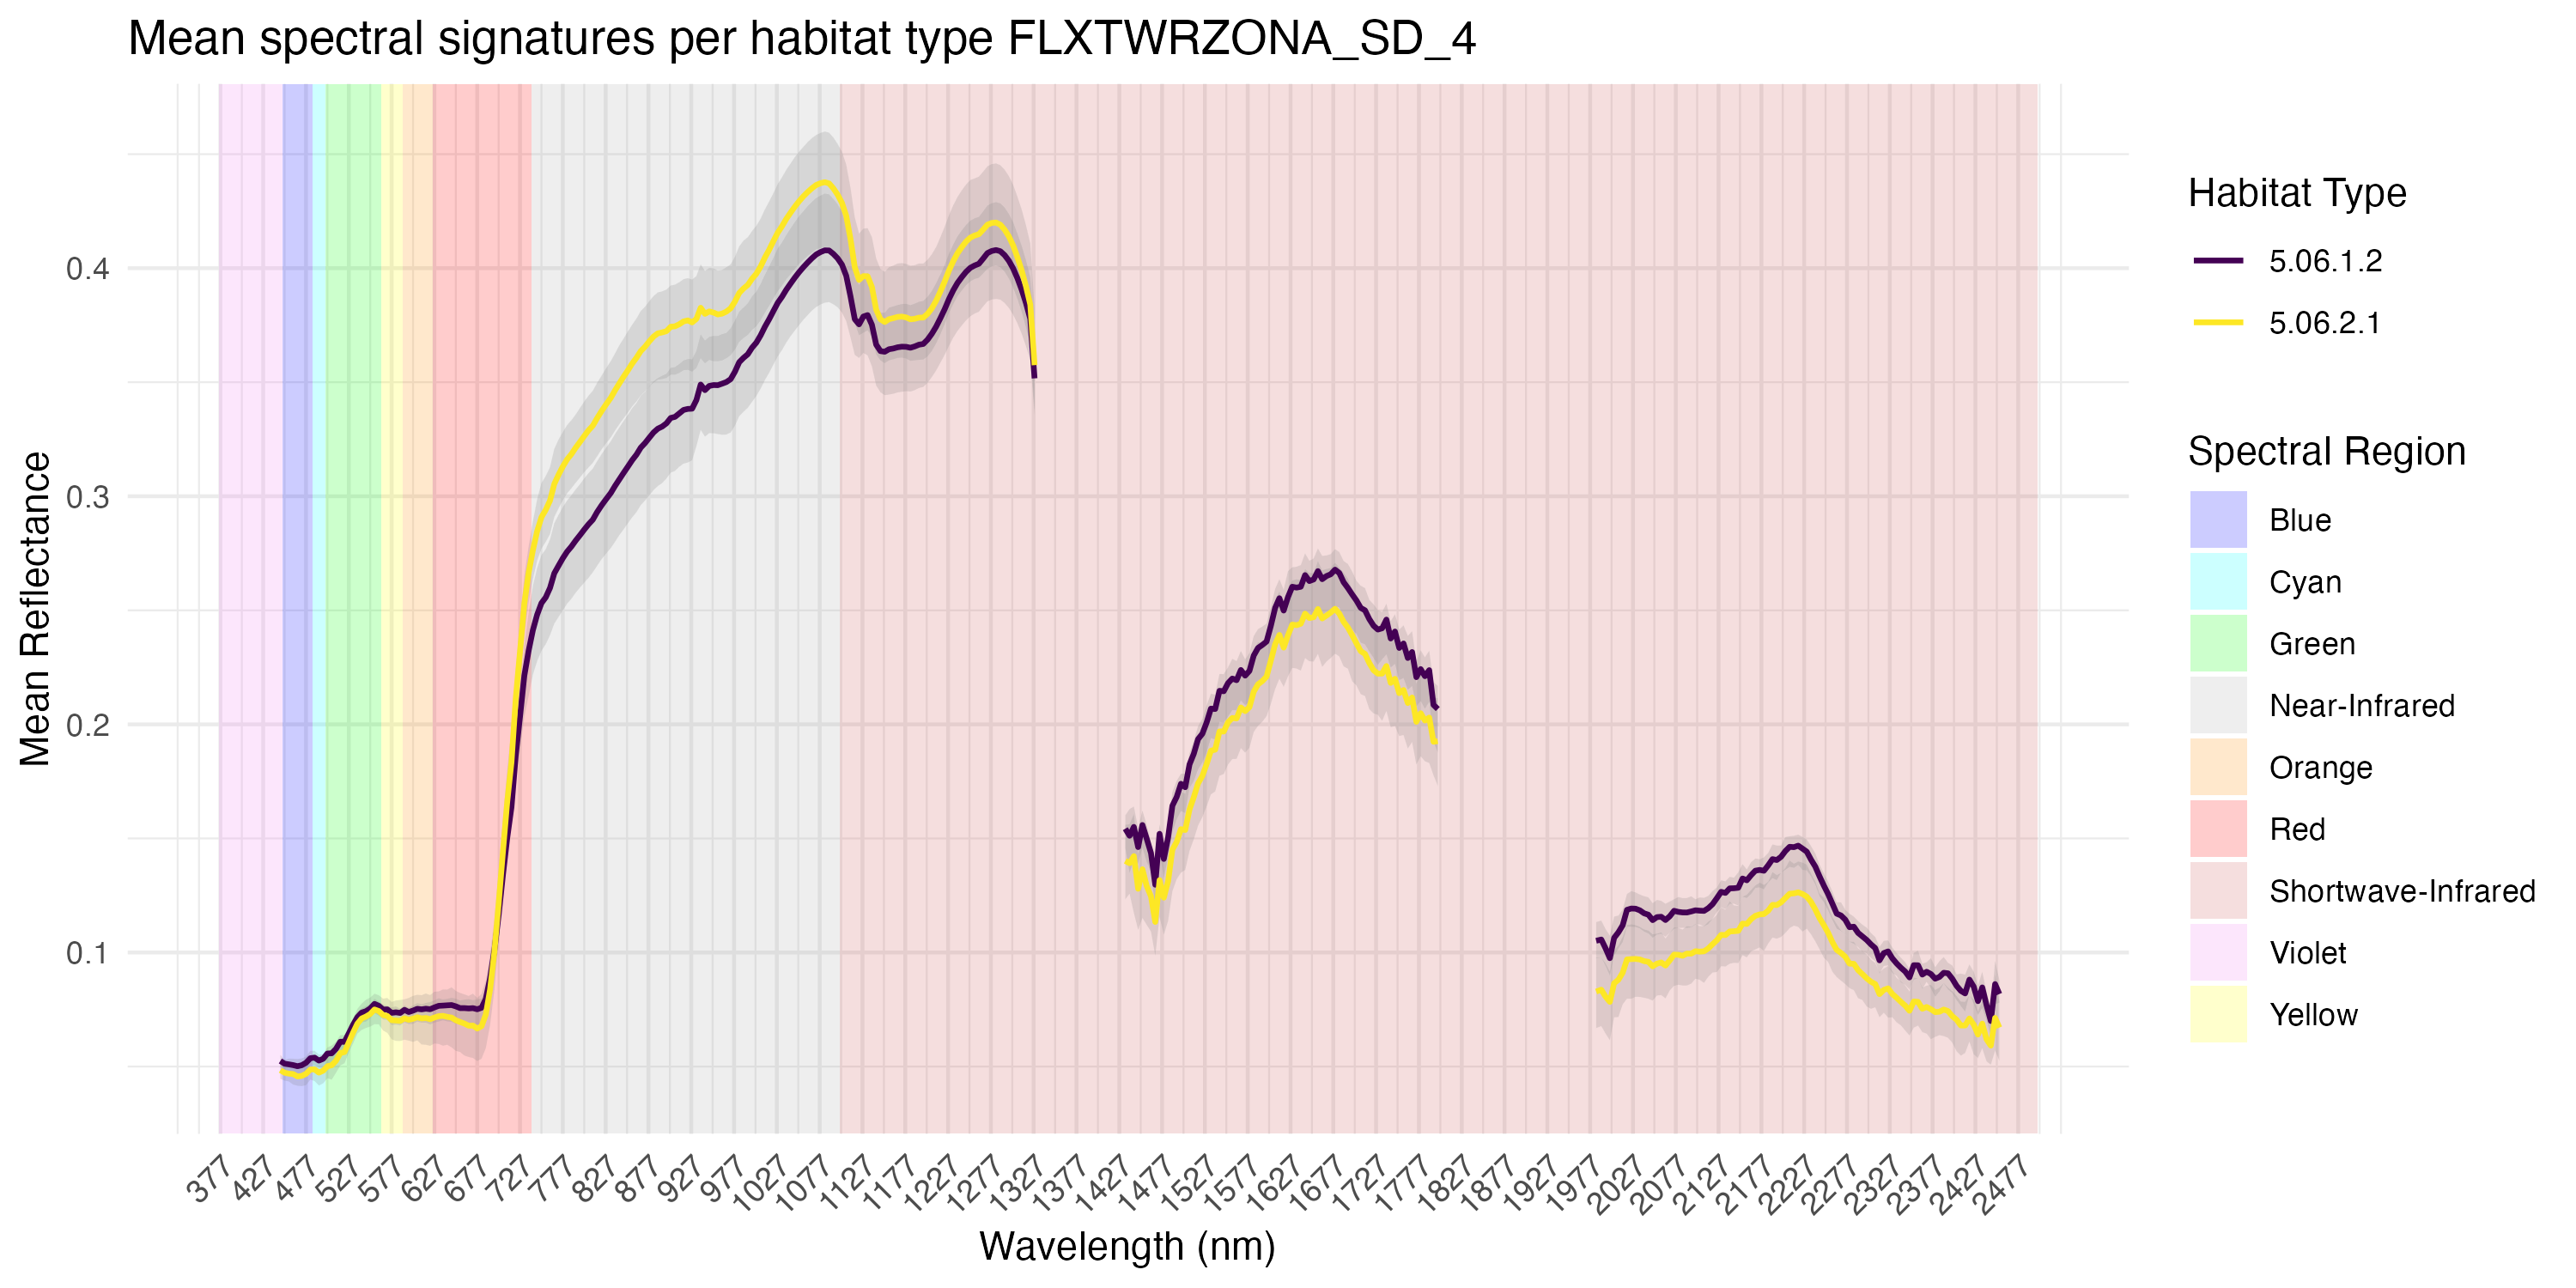
\includegraphics[width=\textwidth]{Figures/spectral_signatures/FLXTWRZONA_SD_4_mean_signature_plot_habitat.png}
    \caption{}
    \label{fig:mss_ht_flxtwrzonasd4}
  \end{subfigure}

  \caption{Spectral signature plot \ref{fig:ss_ht_flxtwrzonasd4} and mean spectral signature plot \ref{fig:mss_ht_flxtwrzonasd4} grouped by habitat type for test site FLXTWRZONA\_SD\_4}
  \label{fig:group_ss_ht_flxtwrzonasd4}
\end{figure}

\begin{figure}[H]
  \centering

  \begin{subfigure}[b]{0.49\textwidth}
    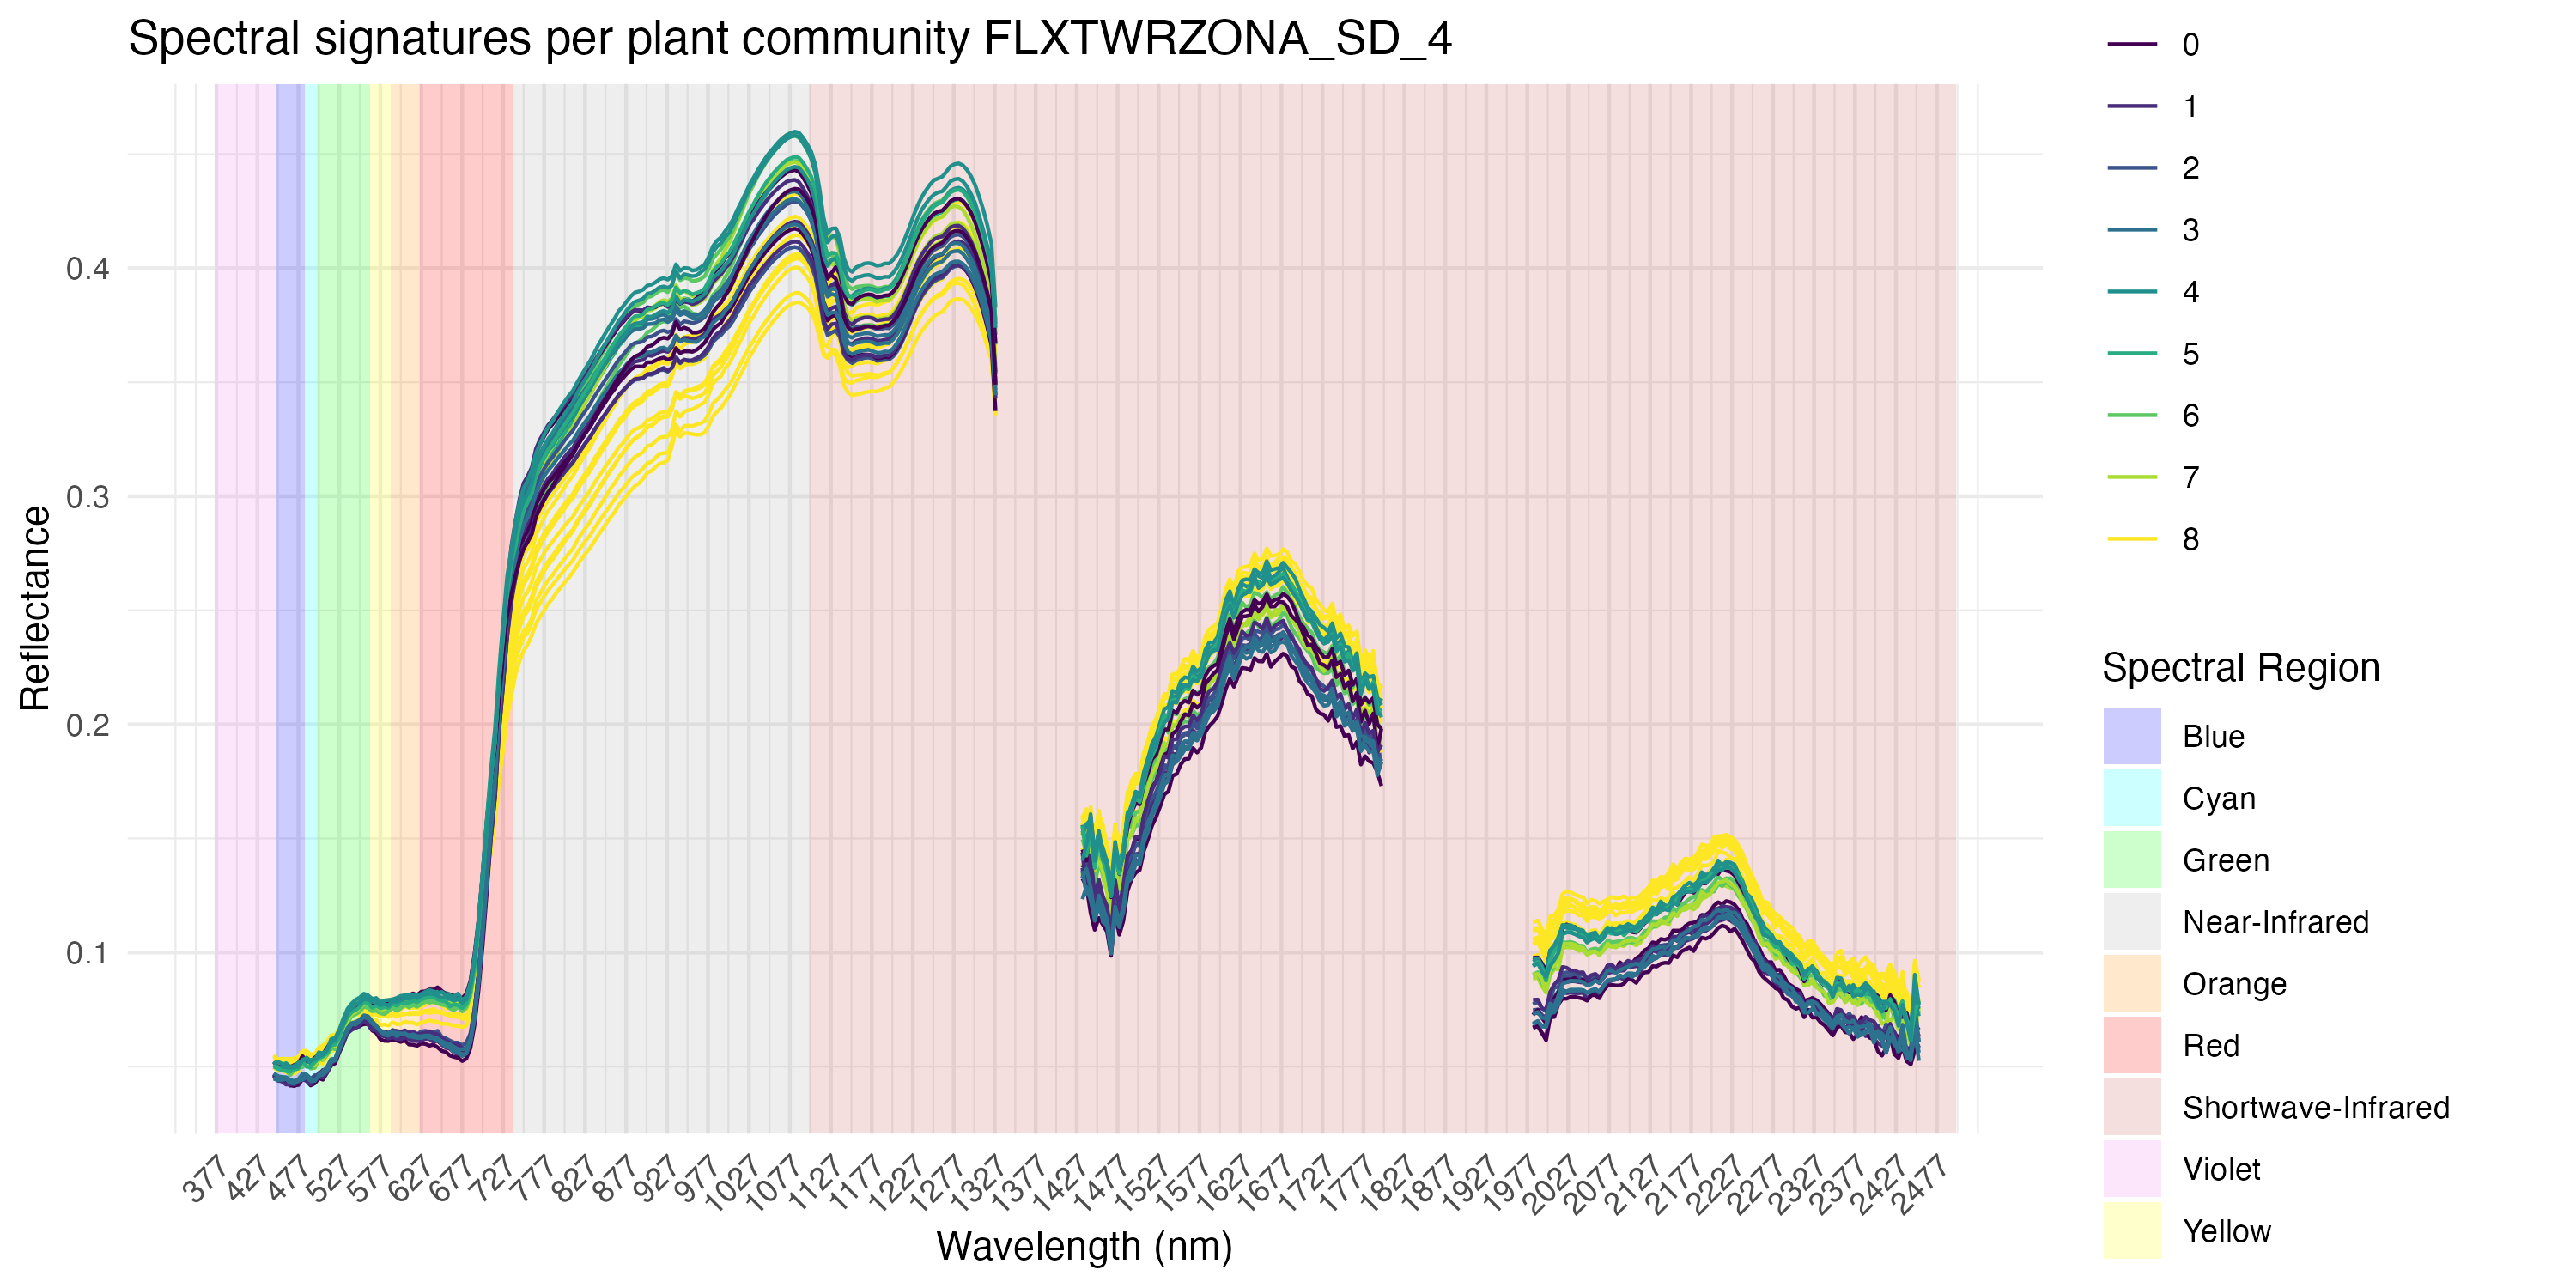
\includegraphics[width=\textwidth]{Figures/spectral_signatures/FLXTWRZONA_SD_4_signature_plot_plant_community.png}
    \caption{}
    \label{fig:ss_pc_flxtwrzonasd4}
  \end{subfigure}
  \hfill
  \begin{subfigure}[b]{0.49\textwidth}
    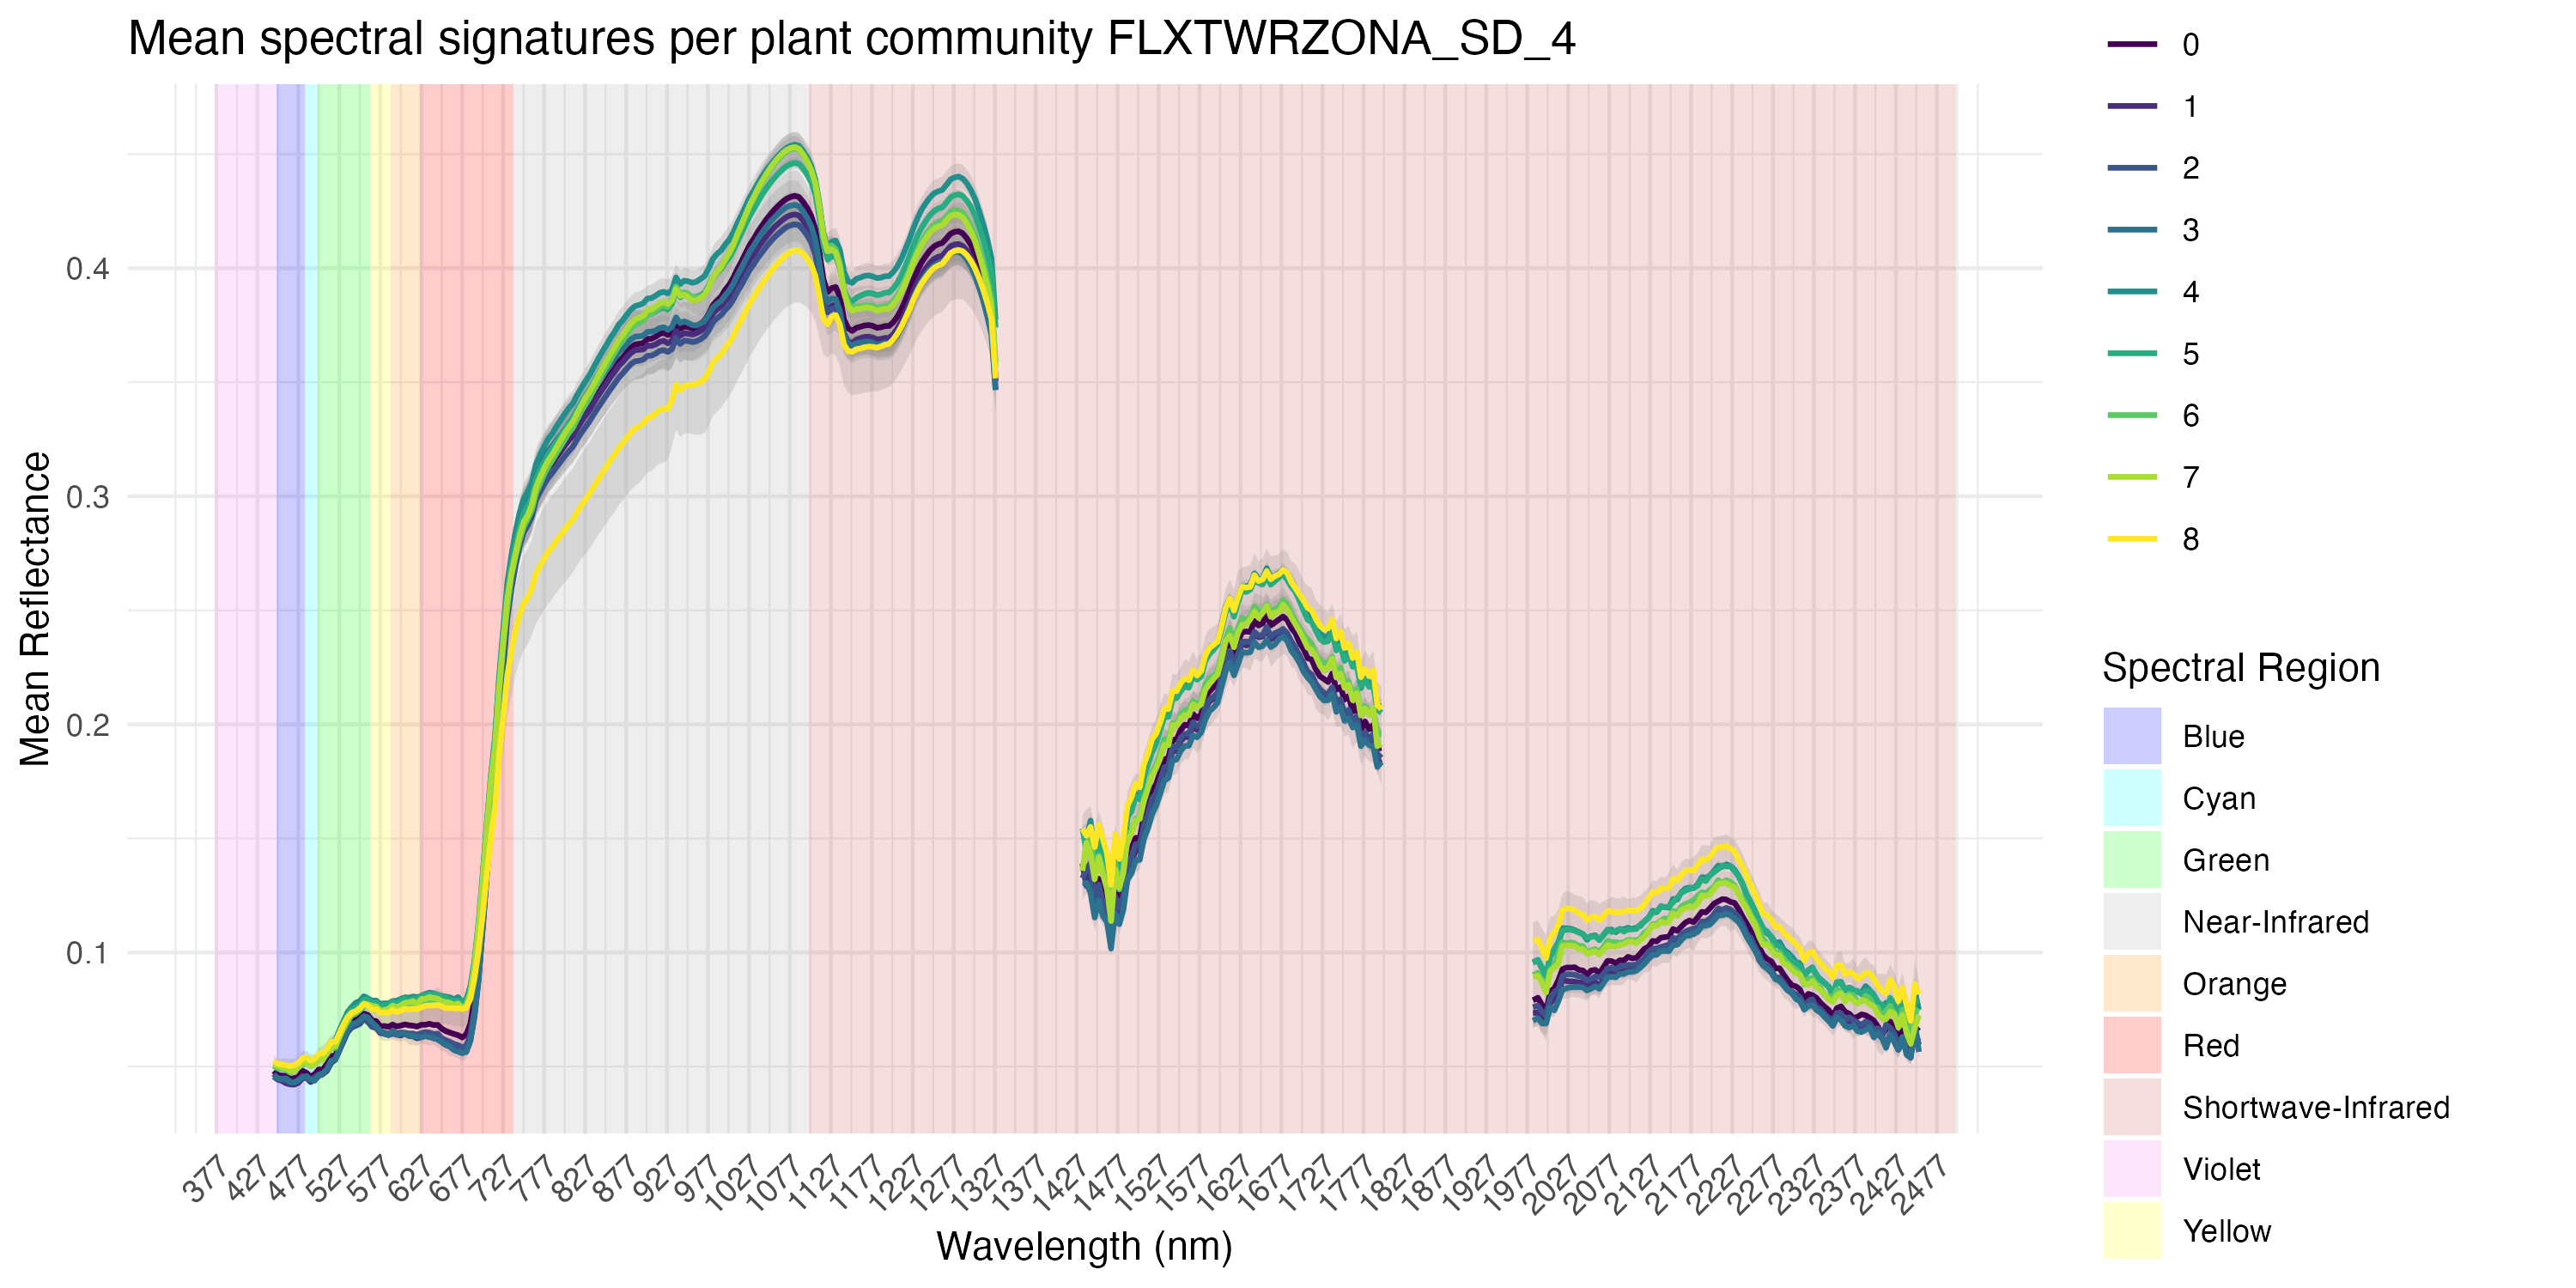
\includegraphics[width=\textwidth]{Figures/spectral_signatures/FLXTWRZONA_SD_4_mean_signature_plot_plant_community.png}
    \caption{}
    \label{fig:mss_pc_flxtwrzonasd4}
  \end{subfigure}

  \caption{Spectral signature plot \ref{fig:ss_pc_flxtwrzonasd4} and mean spectral signature plot \ref{fig:mss_pc_flxtwrzonasd4} grouped by plant community cluster for test site FLXTWRZONA\_SD\_4}
  \label{fig:group_pc_ht_flxtwrzonasd4}
\end{figure}

\subsection{FRST\_AK\_2}

\begin{figure}[H]
  \centering

  \begin{subfigure}[b]{0.49\textwidth}
    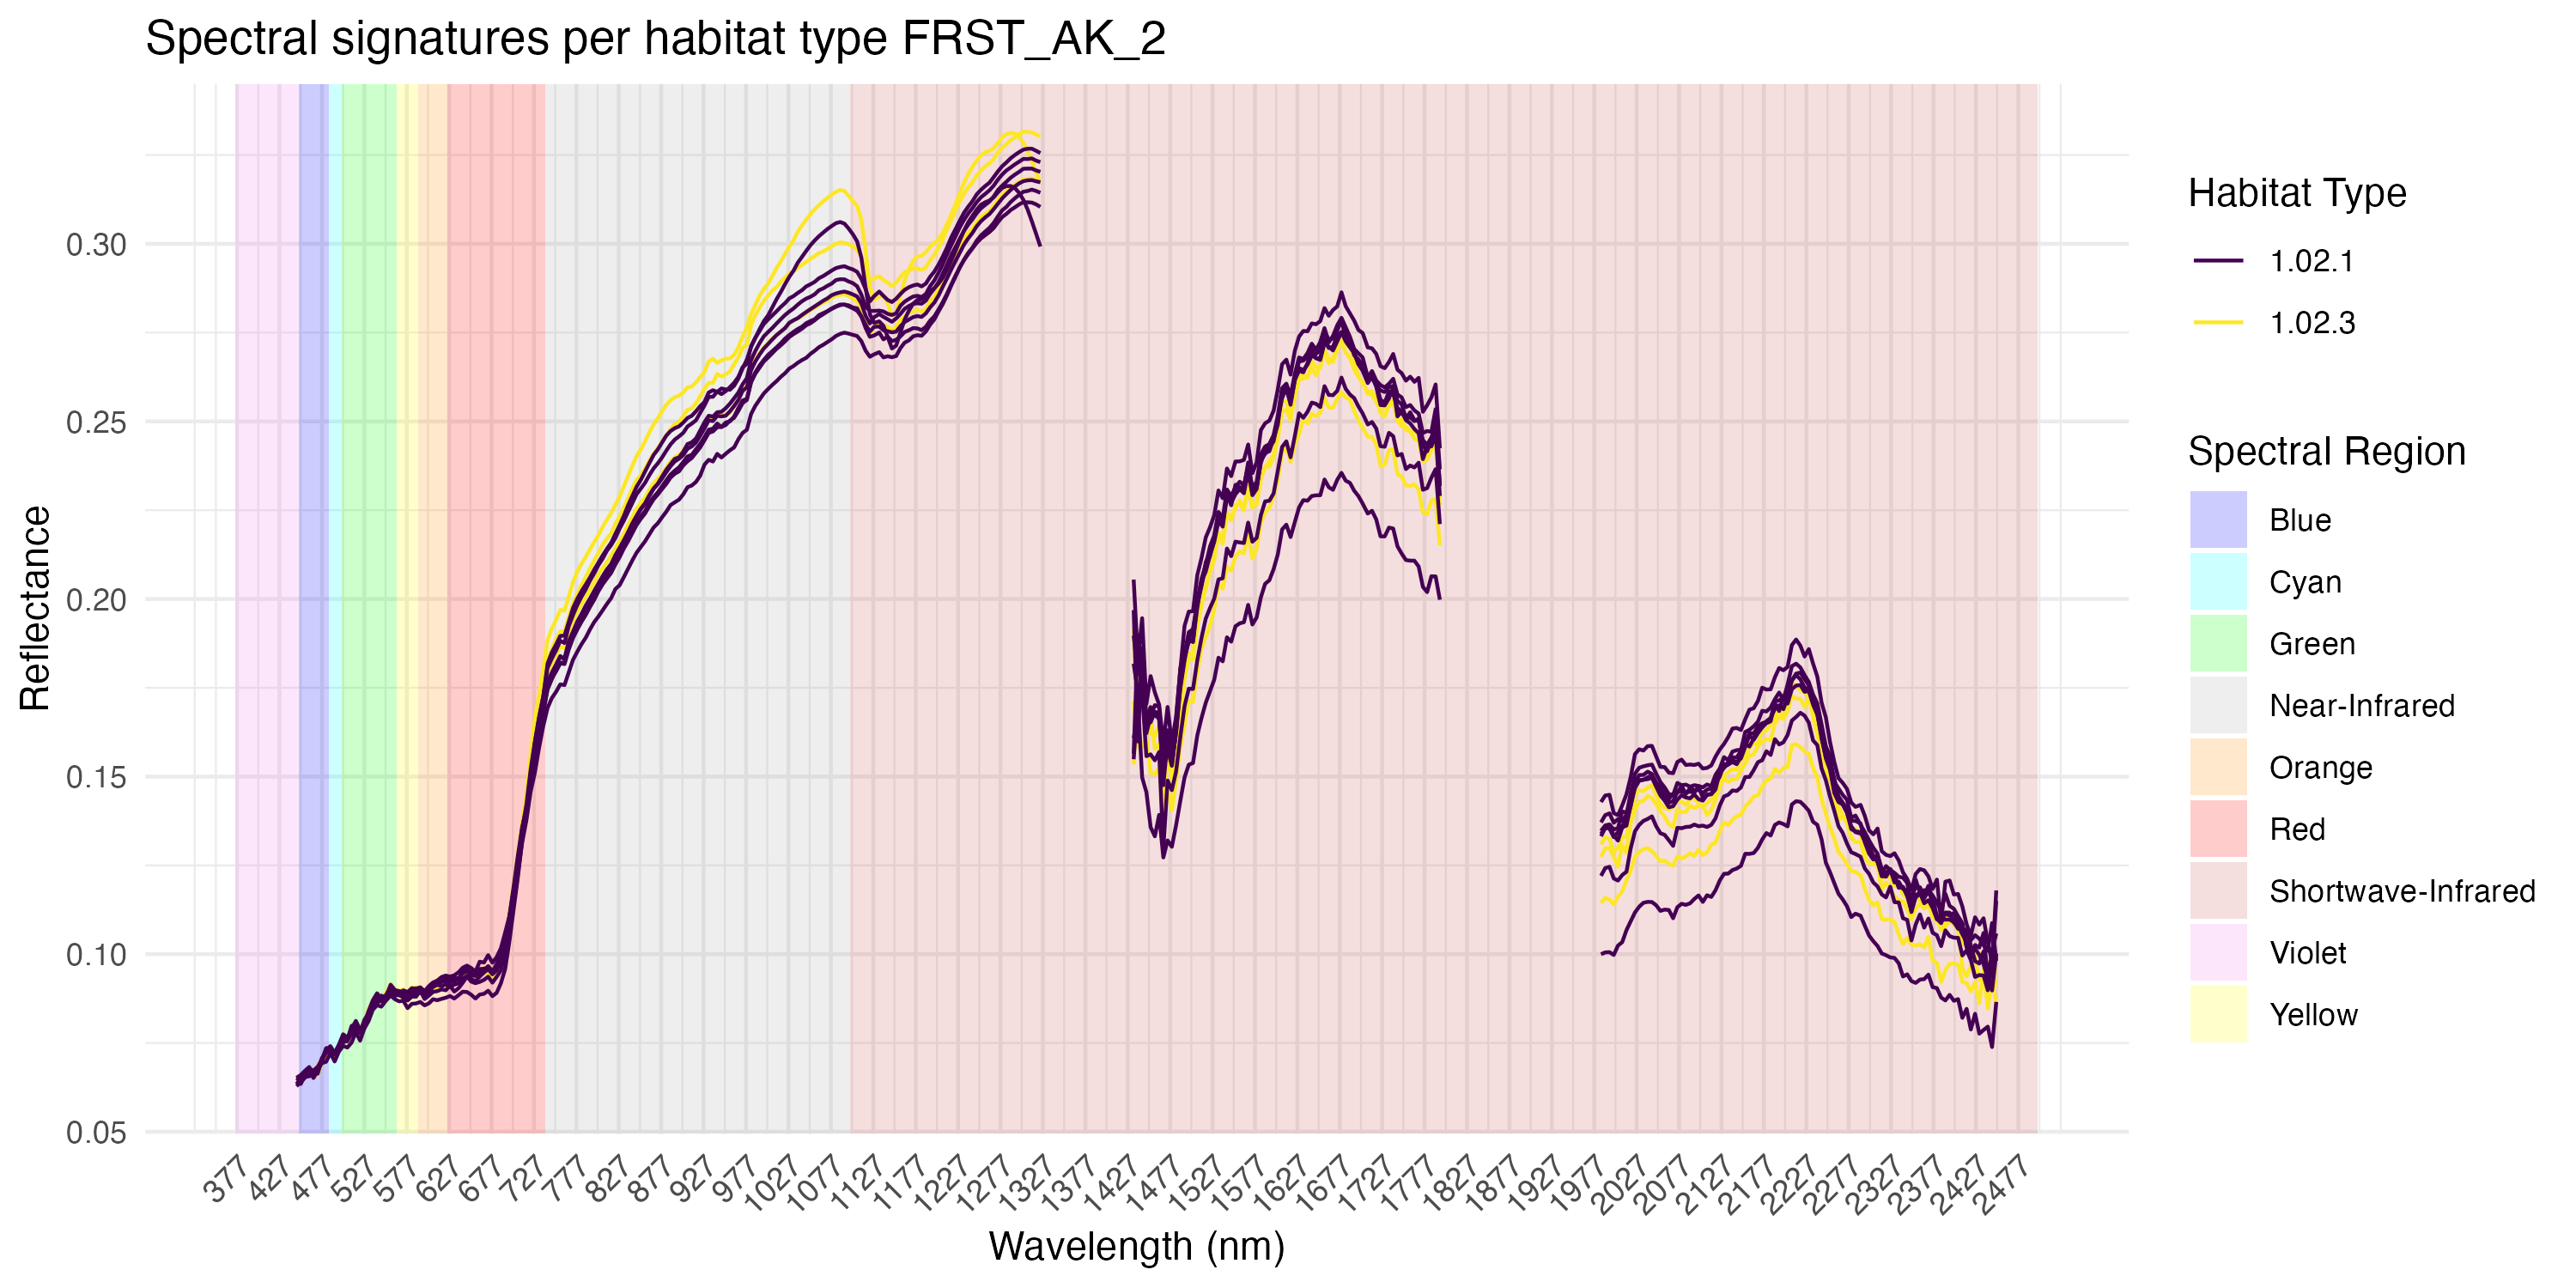
\includegraphics[width=\textwidth]{Figures/spectral_signatures/FRST_AK_2_signature_plot_habitat.png}
    \caption{}
    \label{fig:ss_ht_frstak2}
  \end{subfigure}
  \hfill
  \begin{subfigure}[b]{0.49\textwidth}
    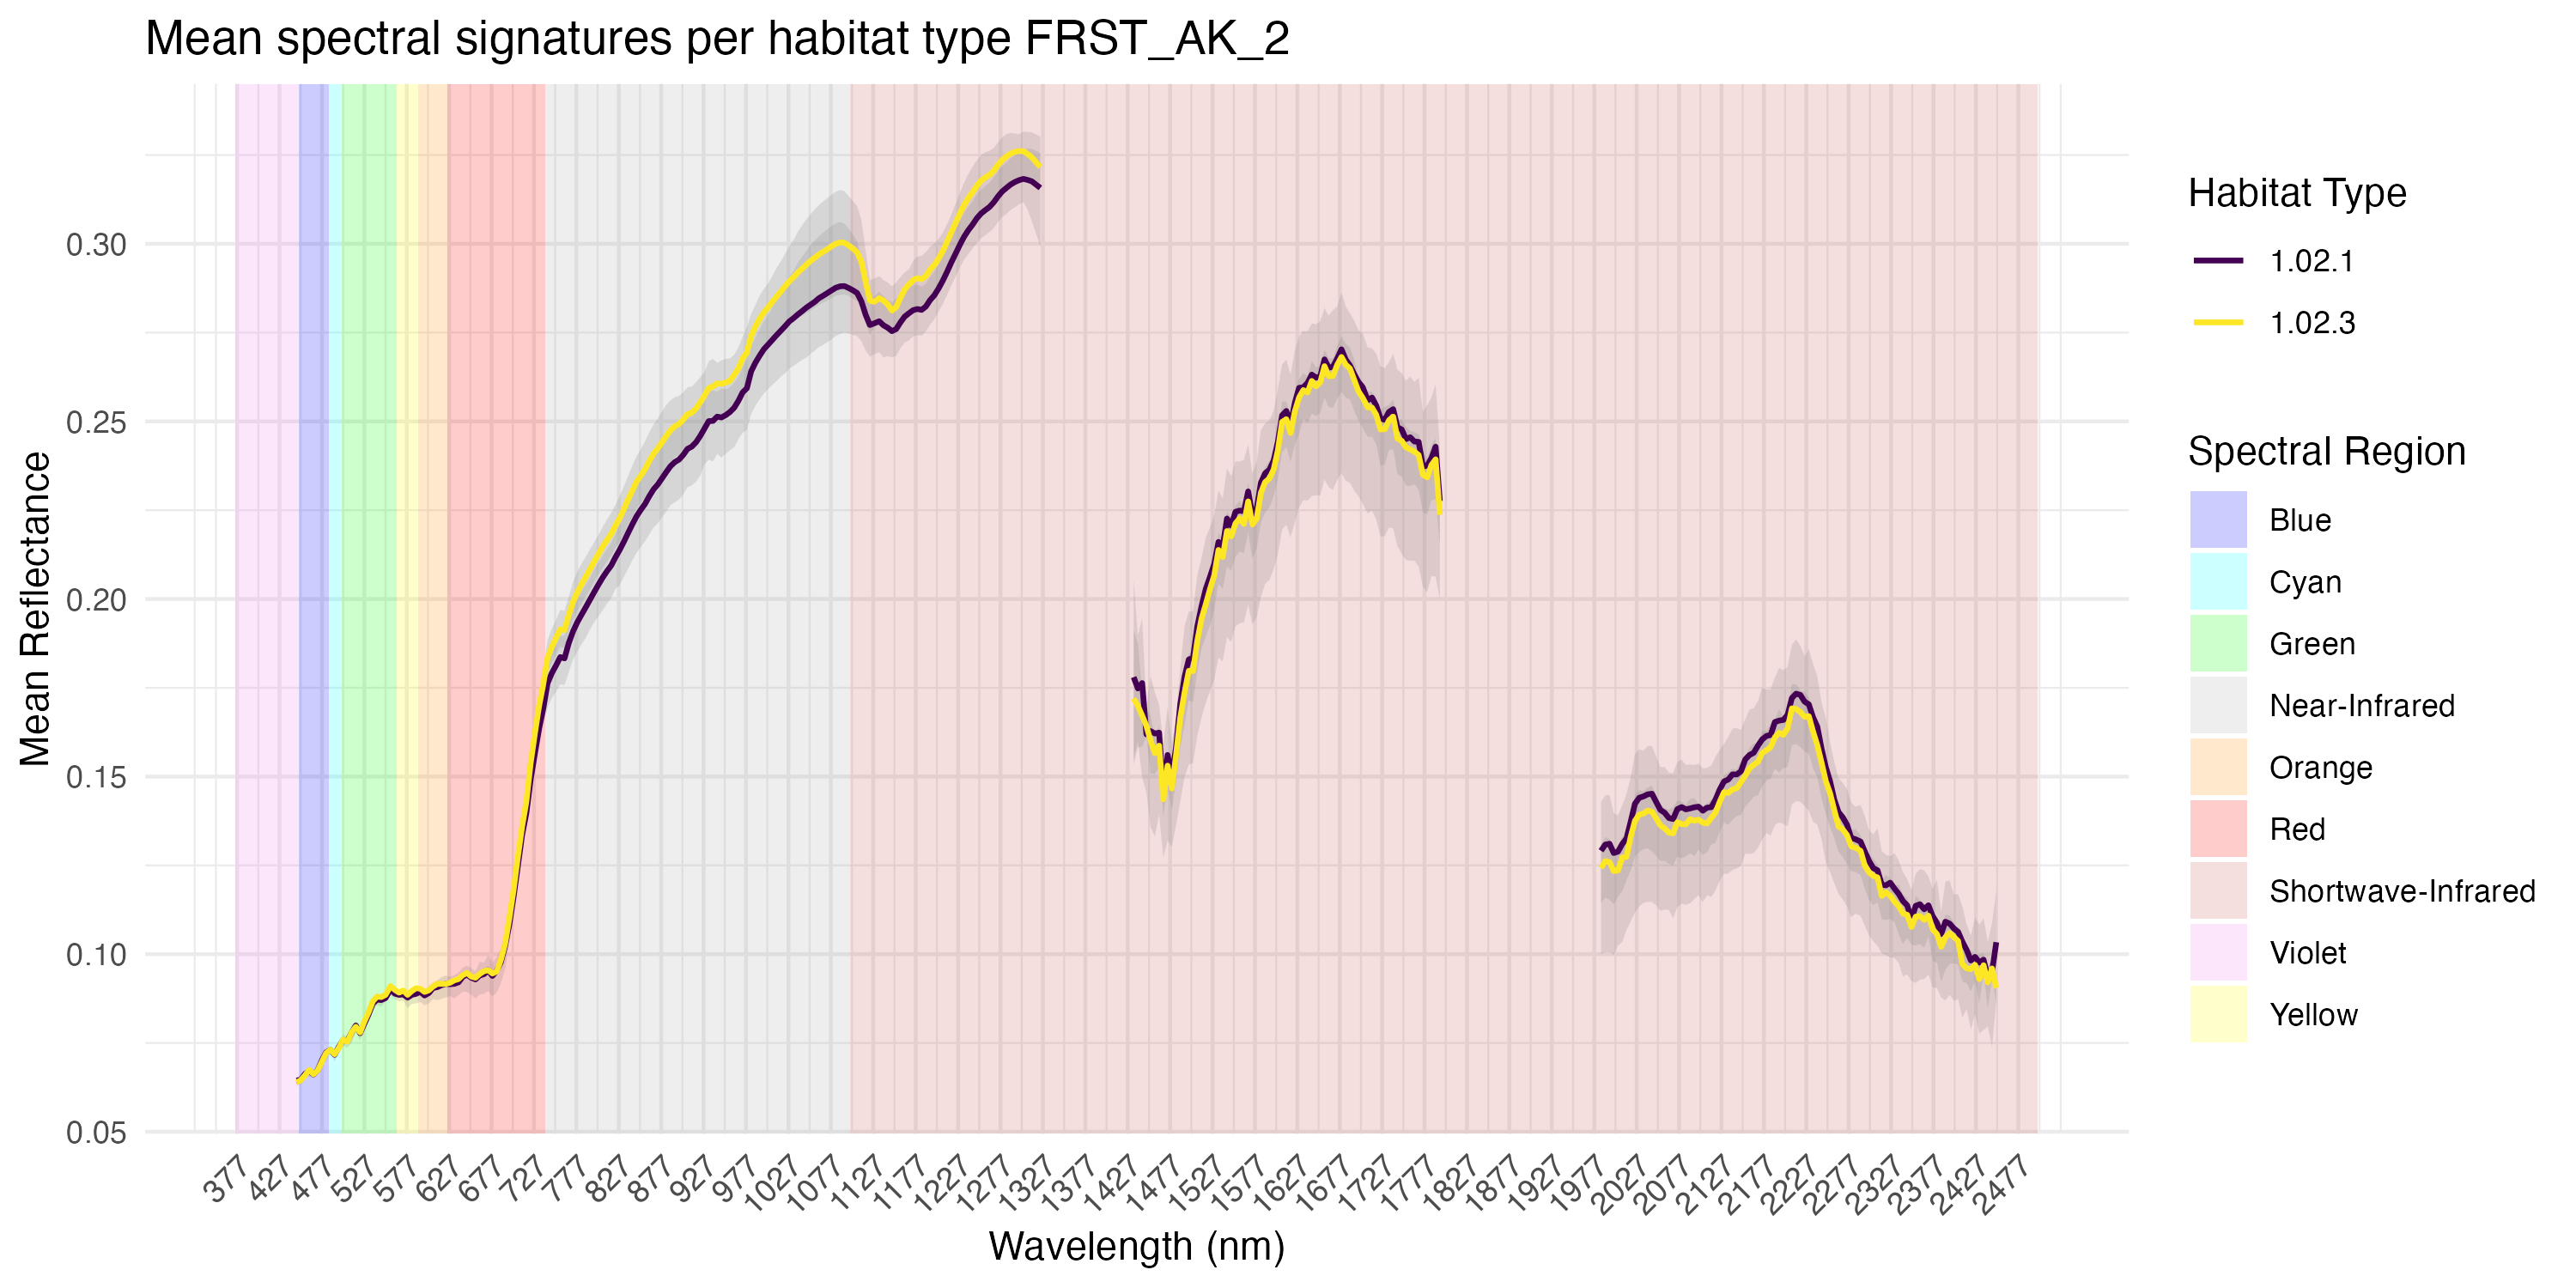
\includegraphics[width=\textwidth]{Figures/spectral_signatures/FRST_AK_2_mean_signature_plot_habitat.png}
    \caption{}
    \label{fig:mss_ht_frstak2}
  \end{subfigure}

  \caption{Spectral signature plot \ref{fig:ss_ht_frstak2} and mean spectral signature plot \ref{fig:mss_ht_frstak2} grouped by habitat type for test site FRST\_AK\_2}
  \label{fig:group_ss_ht_frstak2}
\end{figure}

\begin{figure}[H]
  \centering

  \begin{subfigure}[b]{0.49\textwidth}
    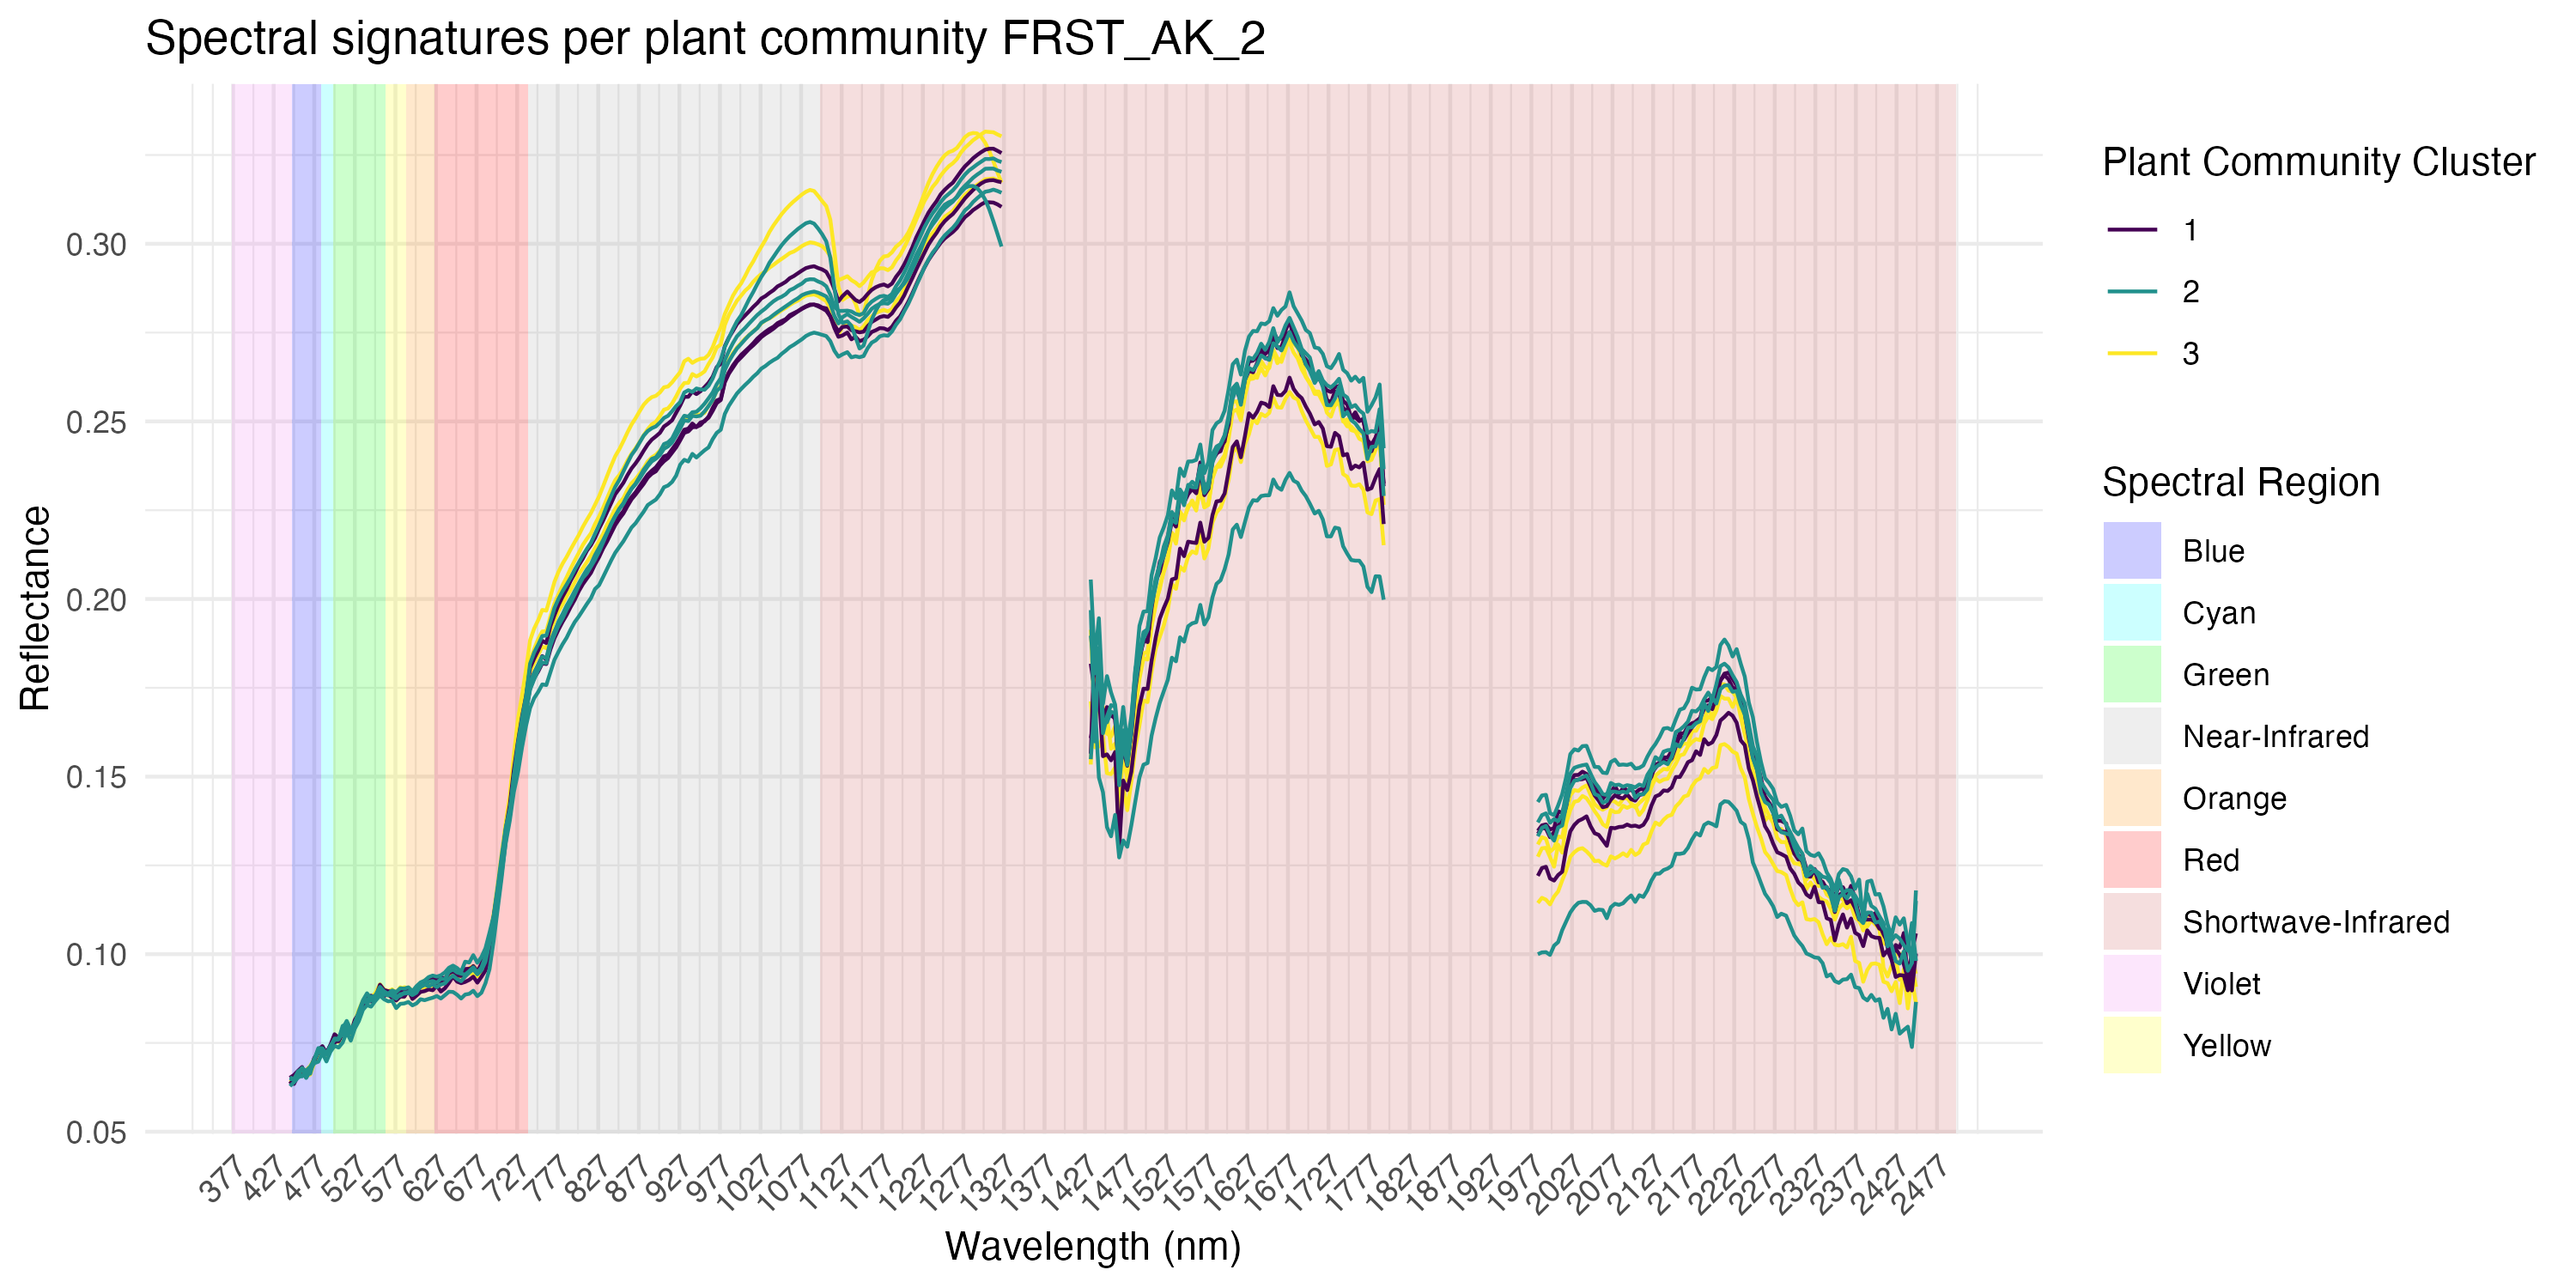
\includegraphics[width=\textwidth]{Figures/spectral_signatures/FRST_AK_2_signature_plot_plant_community.png}
    \caption{}
    \label{fig:ss_pc_frstak2}
  \end{subfigure}
  \hfill
  \begin{subfigure}[b]{0.49\textwidth}
    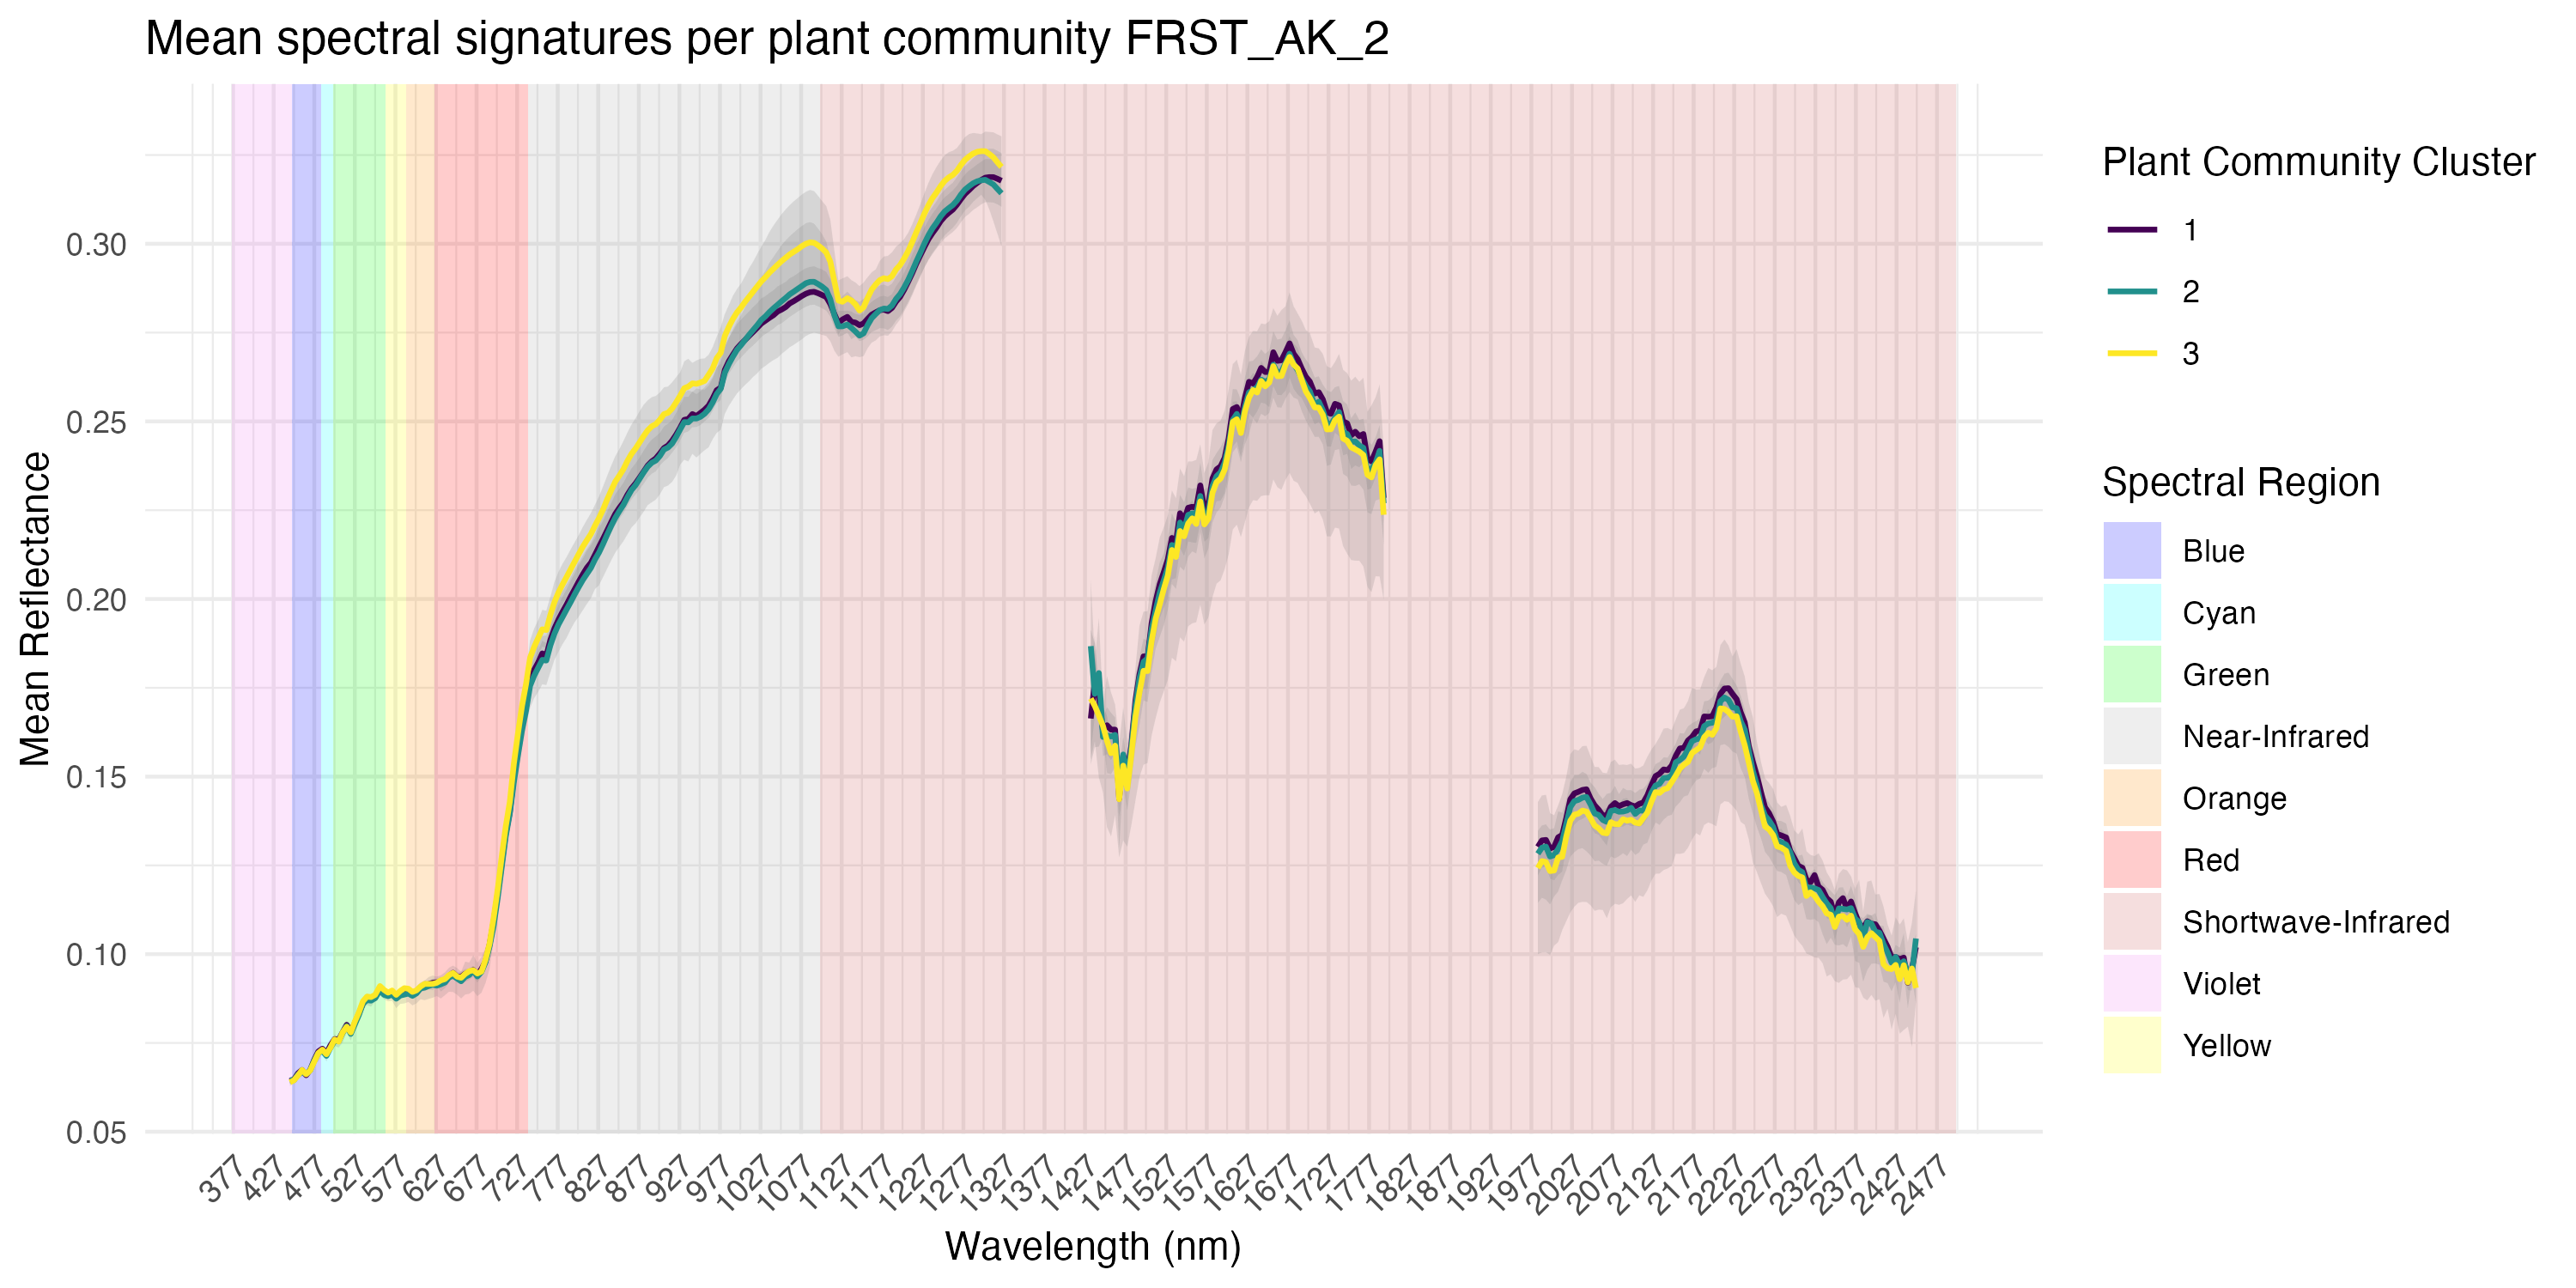
\includegraphics[width=\textwidth]{Figures/spectral_signatures/FRST_AK_2_mean_signature_plot_plant_community.png}
    \caption{}
    \label{fig:mss_pc_frstak2}
  \end{subfigure}

  \caption{Spectral signature plot \ref{fig:ss_pc_frstak2} and mean spectral signature plot \ref{fig:mss_pc_frstak2} grouped by plant community cluster for test site FRST\_AK\_2}
  \label{fig:group_pc_ht_frstak2}
\end{figure}

\subsection{FRST\_AK\_3}

\begin{figure}[H]
  \centering

  \begin{subfigure}[b]{0.49\textwidth}
    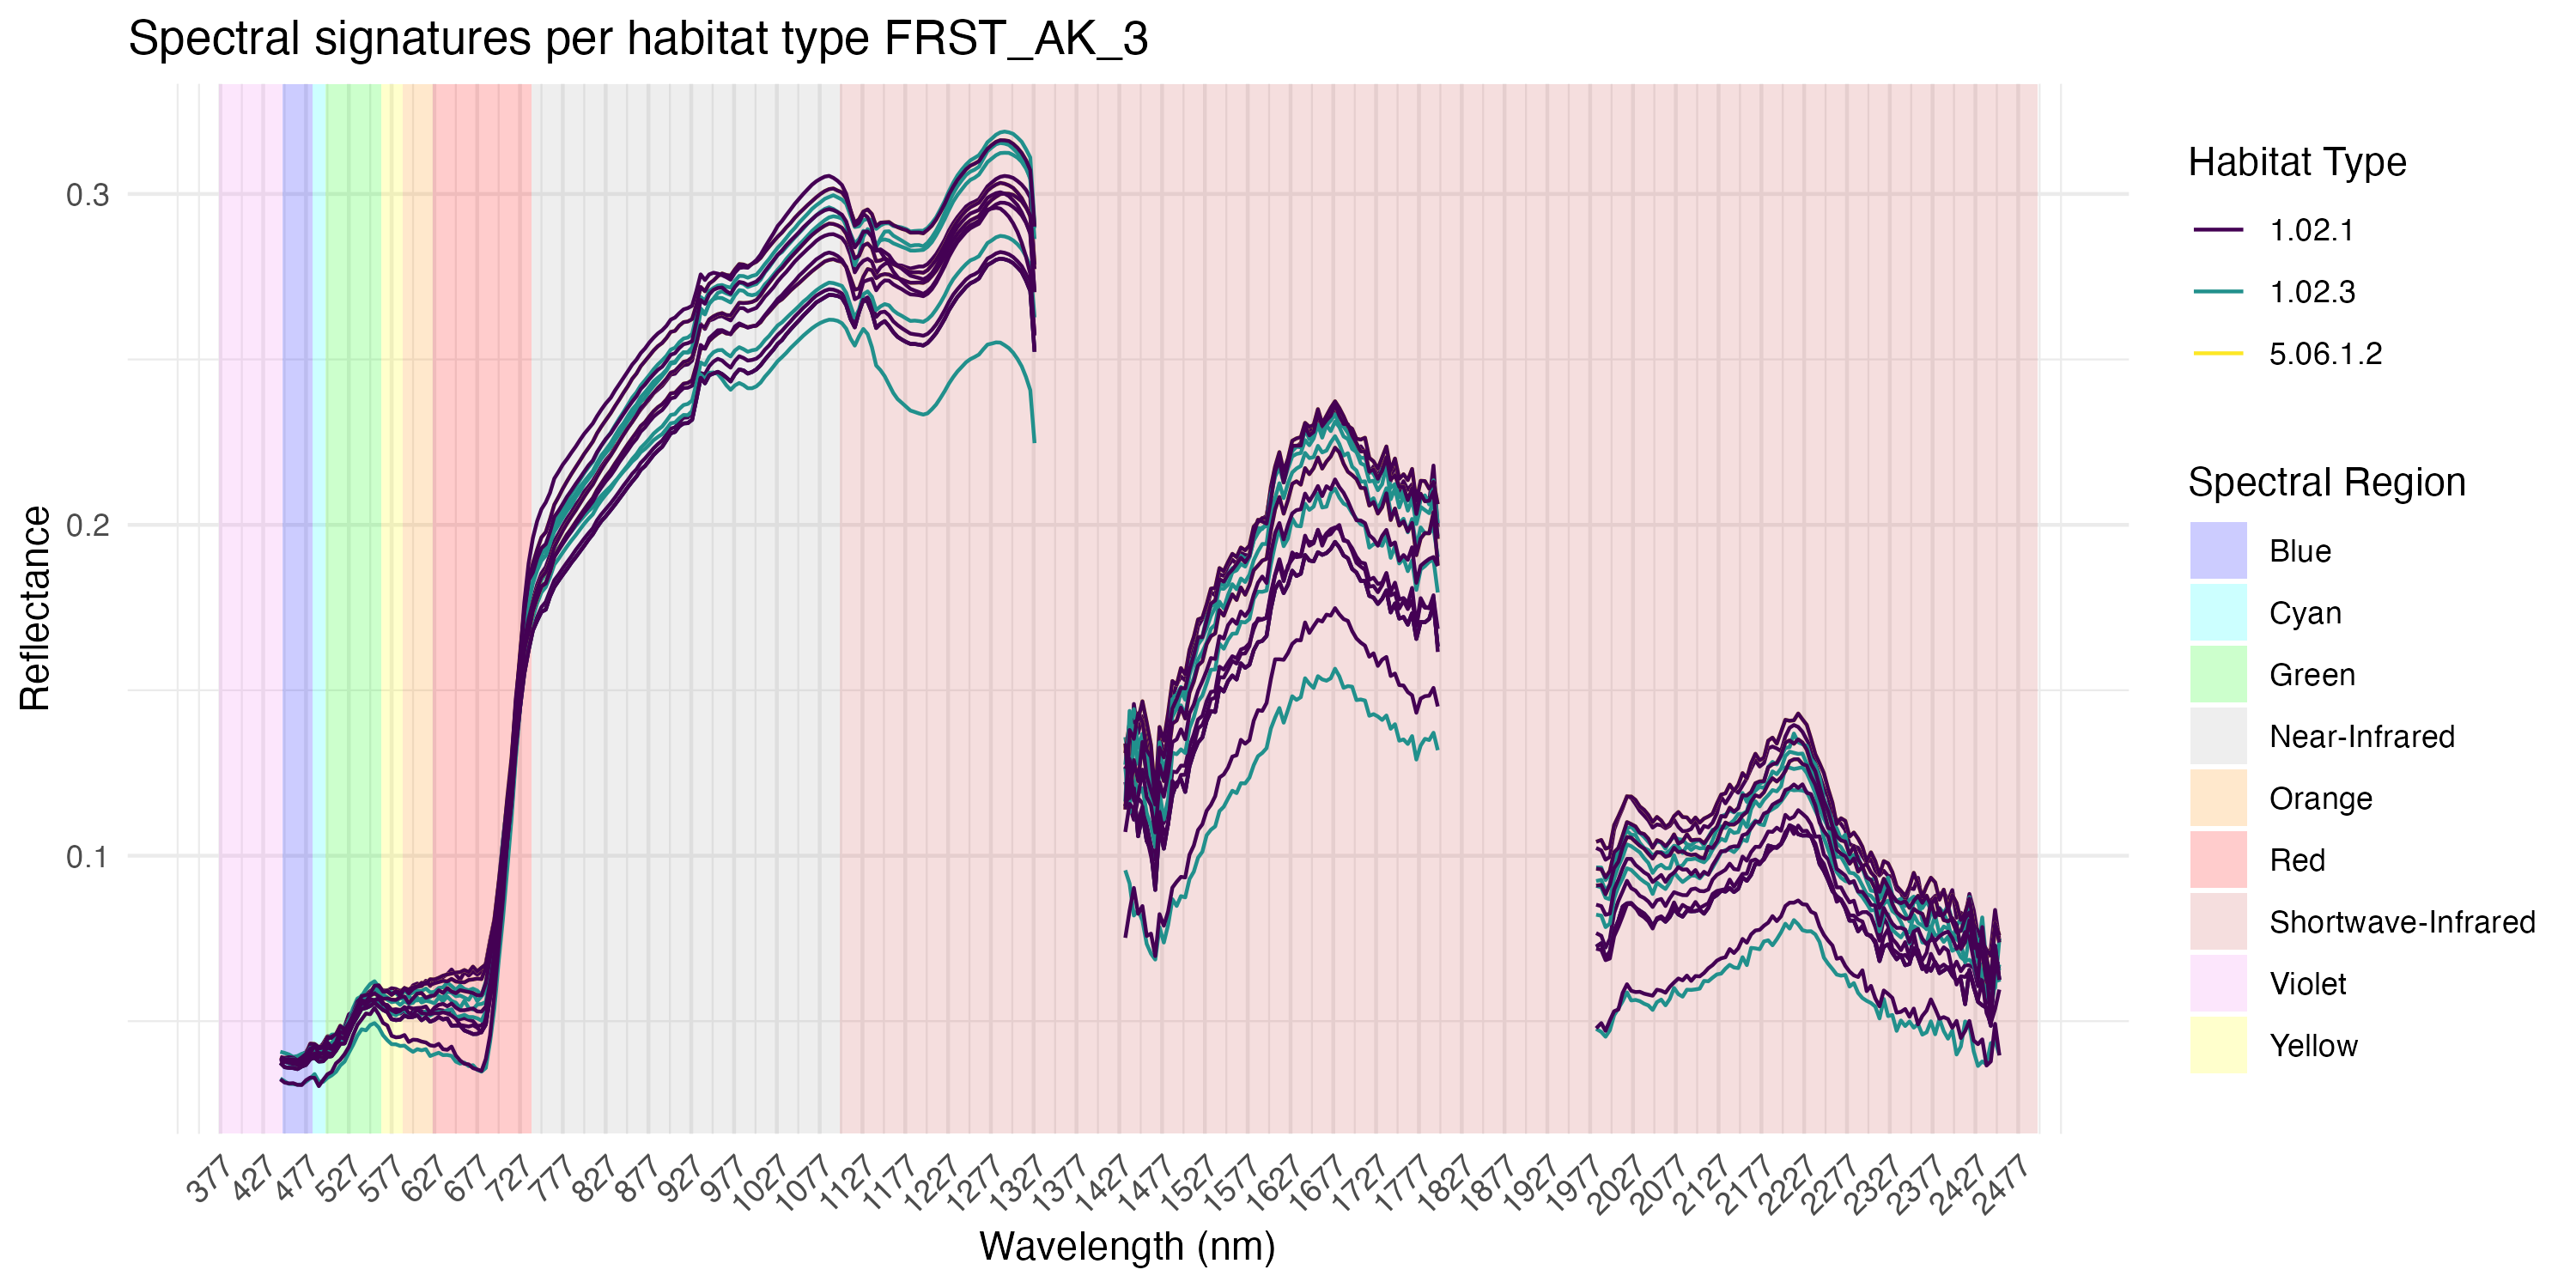
\includegraphics[width=\textwidth]{Figures/spectral_signatures/FRST_AK_3_signature_plot_habitat.png}
    \caption{}
    \label{fig:ss_ht_frstak3}
  \end{subfigure}
  \hfill
  \begin{subfigure}[b]{0.49\textwidth}
    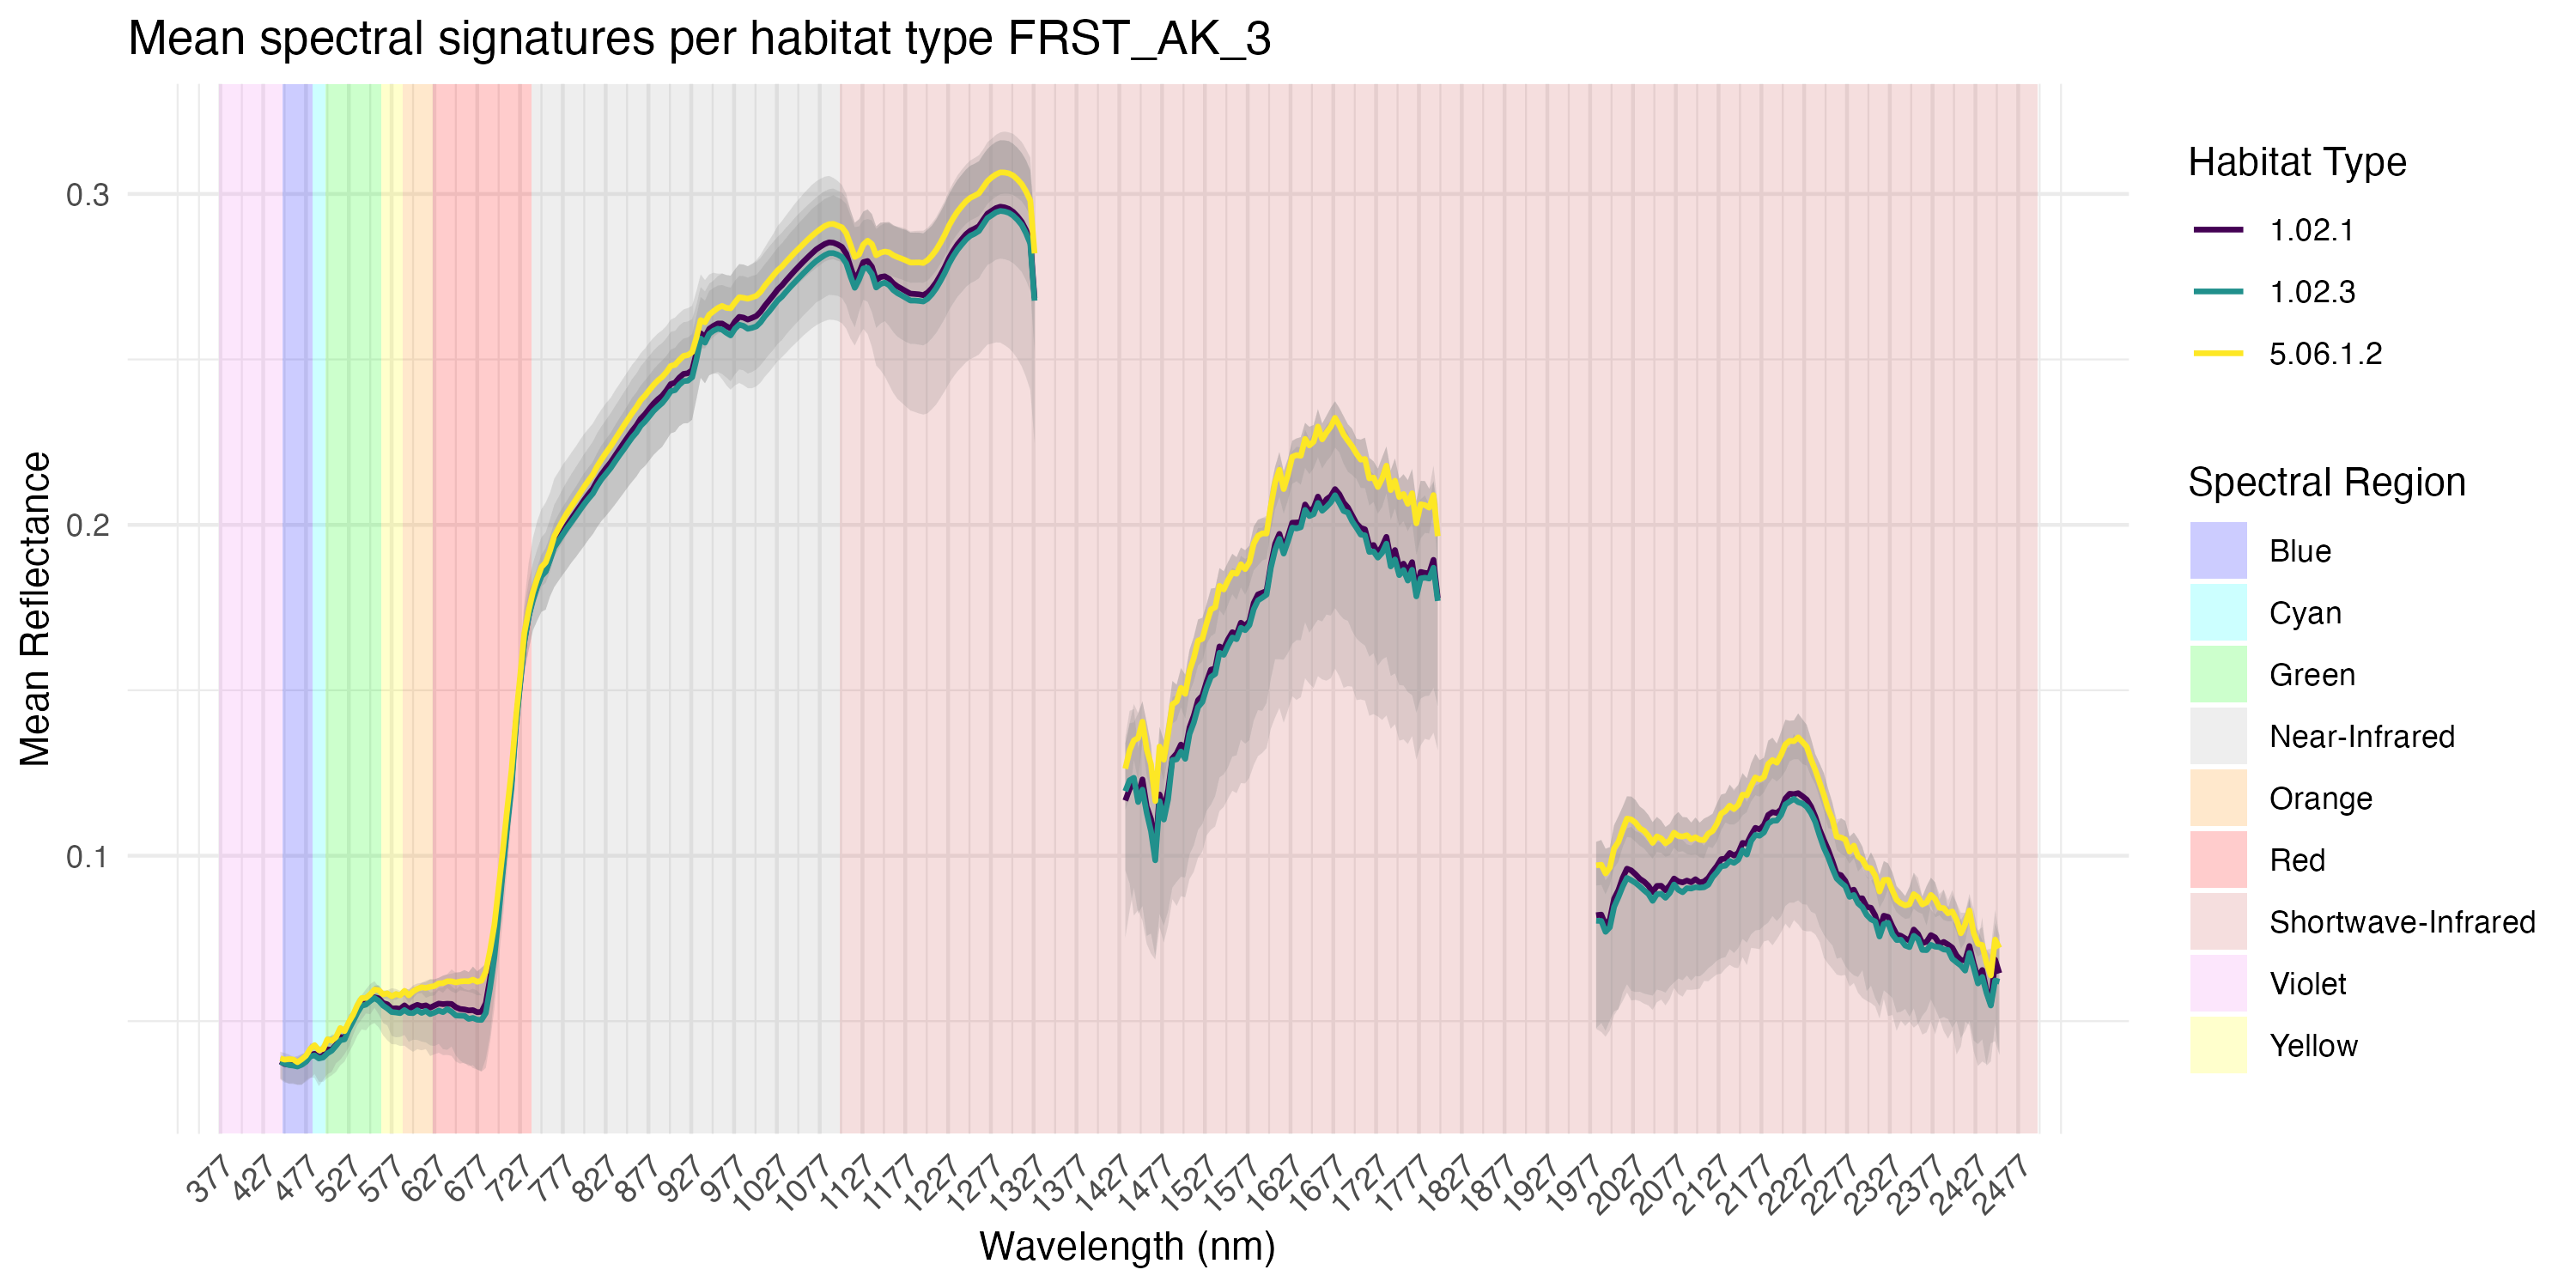
\includegraphics[width=\textwidth]{Figures/spectral_signatures/FRST_AK_3_mean_signature_plot_habitat.png}
    \caption{}
    \label{fig:mss_ht_frstak3}
  \end{subfigure}

  \caption{Spectral signature plot \ref{fig:ss_ht_frstak3} and mean spectral signature plot \ref{fig:mss_ht_frstak3} grouped by habitat type for test site FRST\_AK\_3}
  \label{fig:group_ss_ht_frstak3}
\end{figure}

\begin{figure}[H]
  \centering

  \begin{subfigure}[b]{0.49\textwidth}
    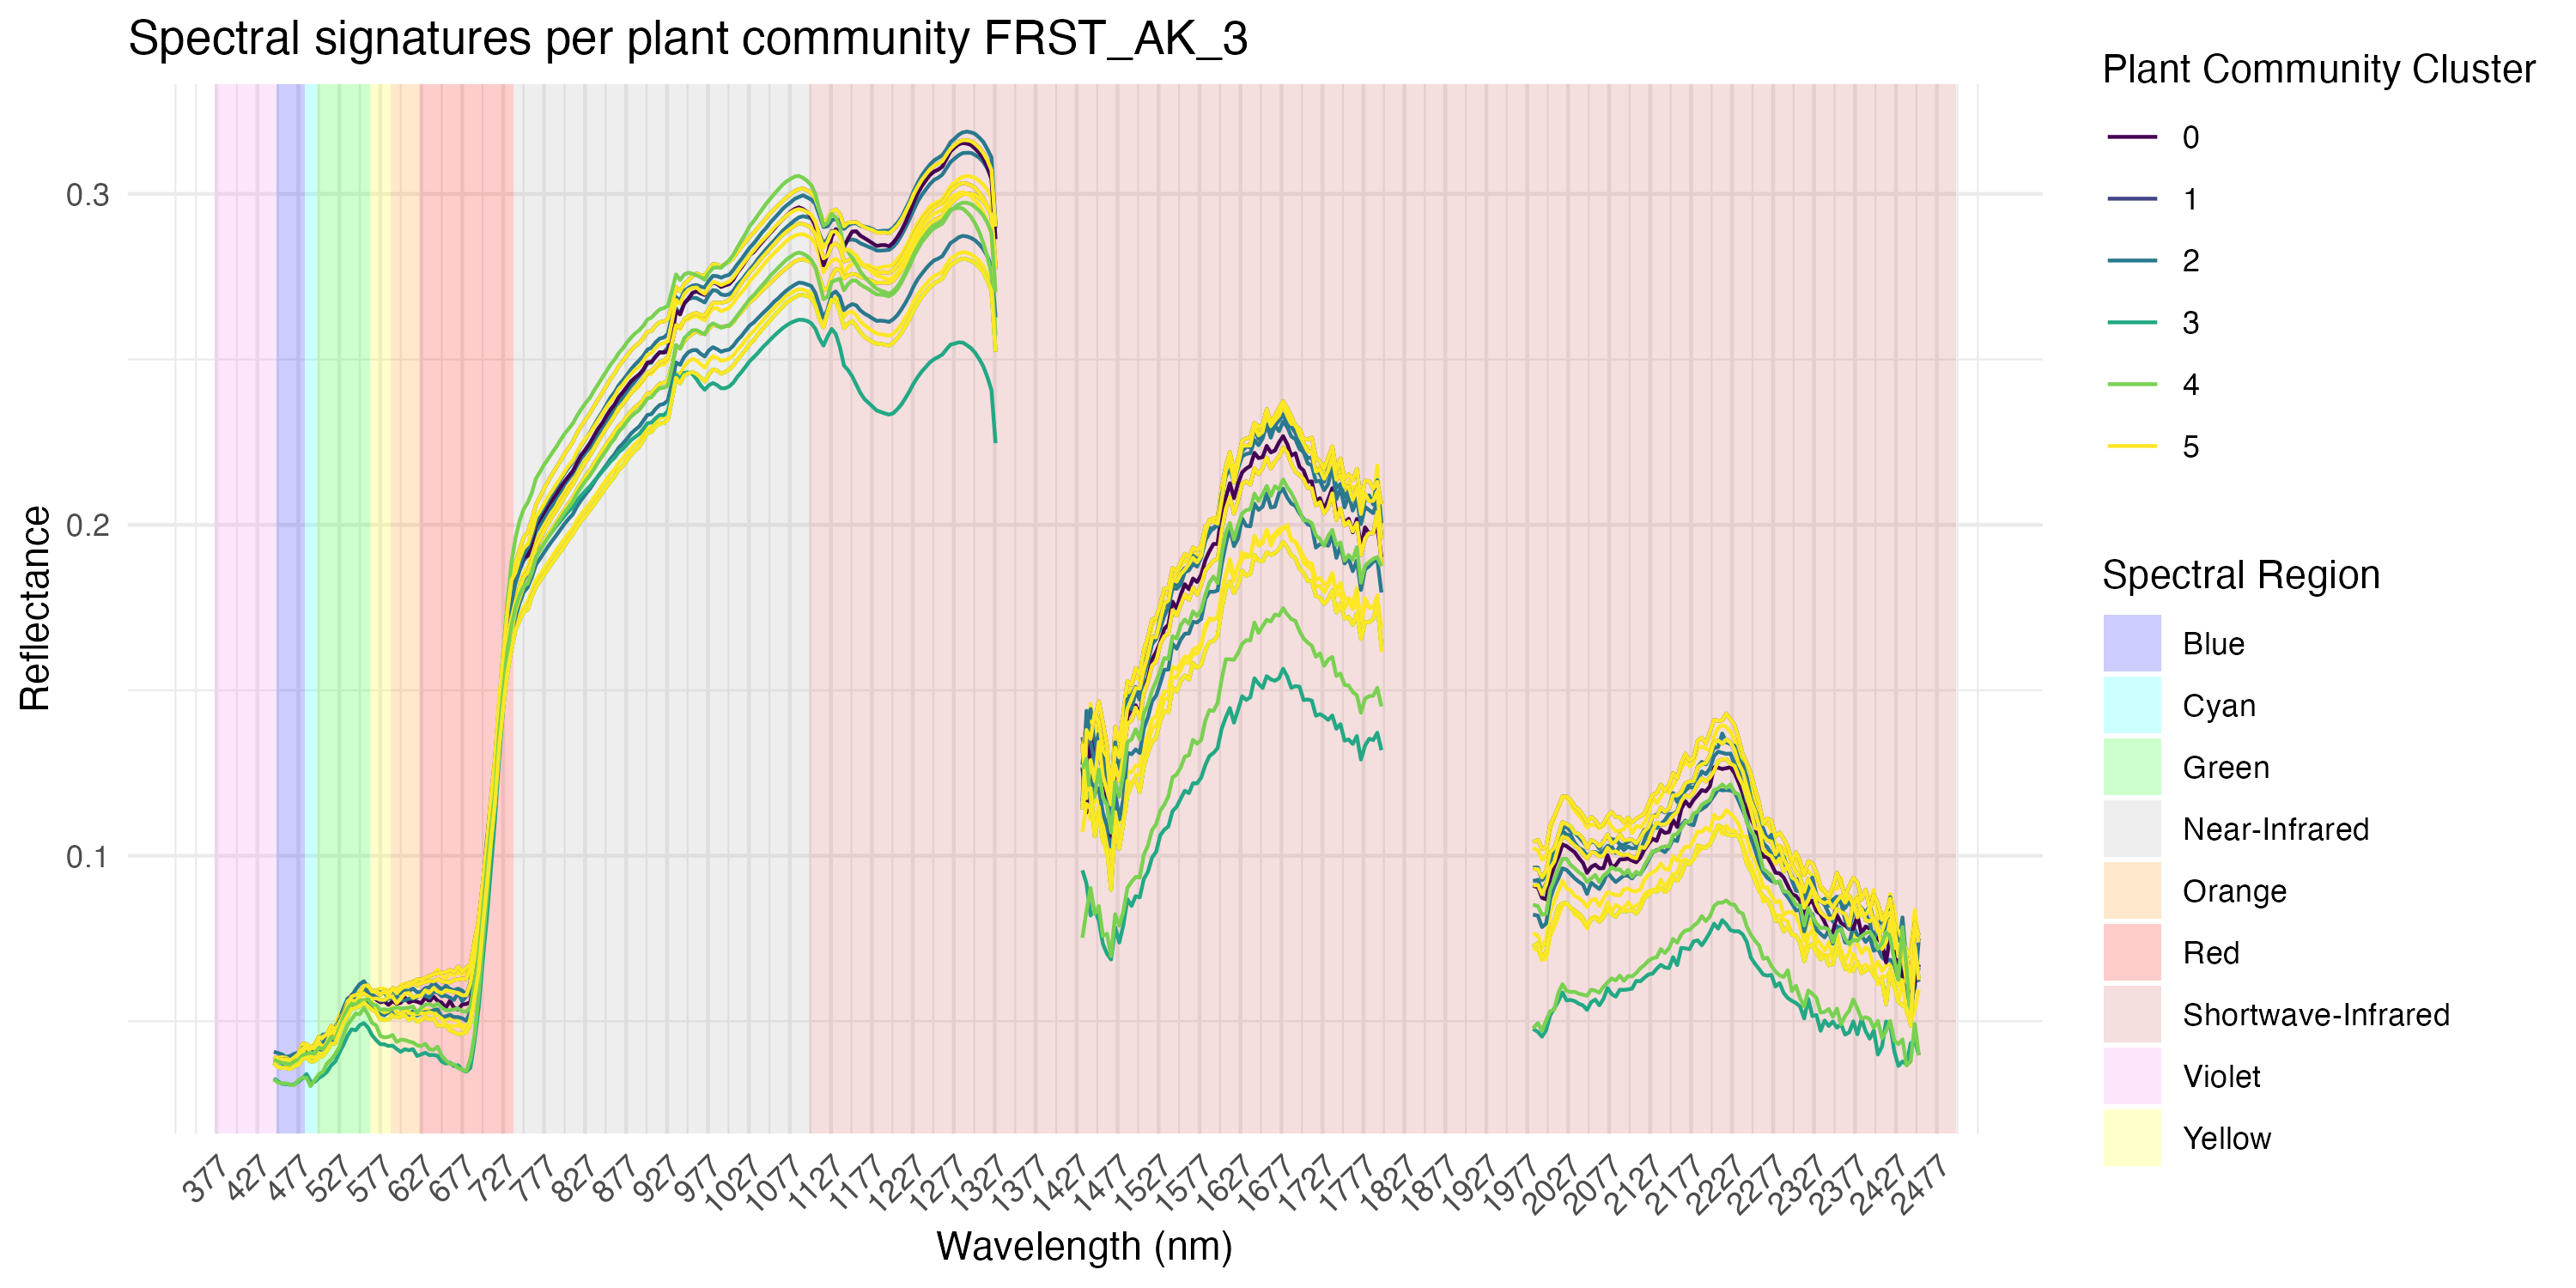
\includegraphics[width=\textwidth]{Figures/spectral_signatures/FRST_AK_3_signature_plot_plant_community.png}
    \caption{}
    \label{fig:ss_pc_frstak3}
  \end{subfigure}
  \hfill
  \begin{subfigure}[b]{0.49\textwidth}
    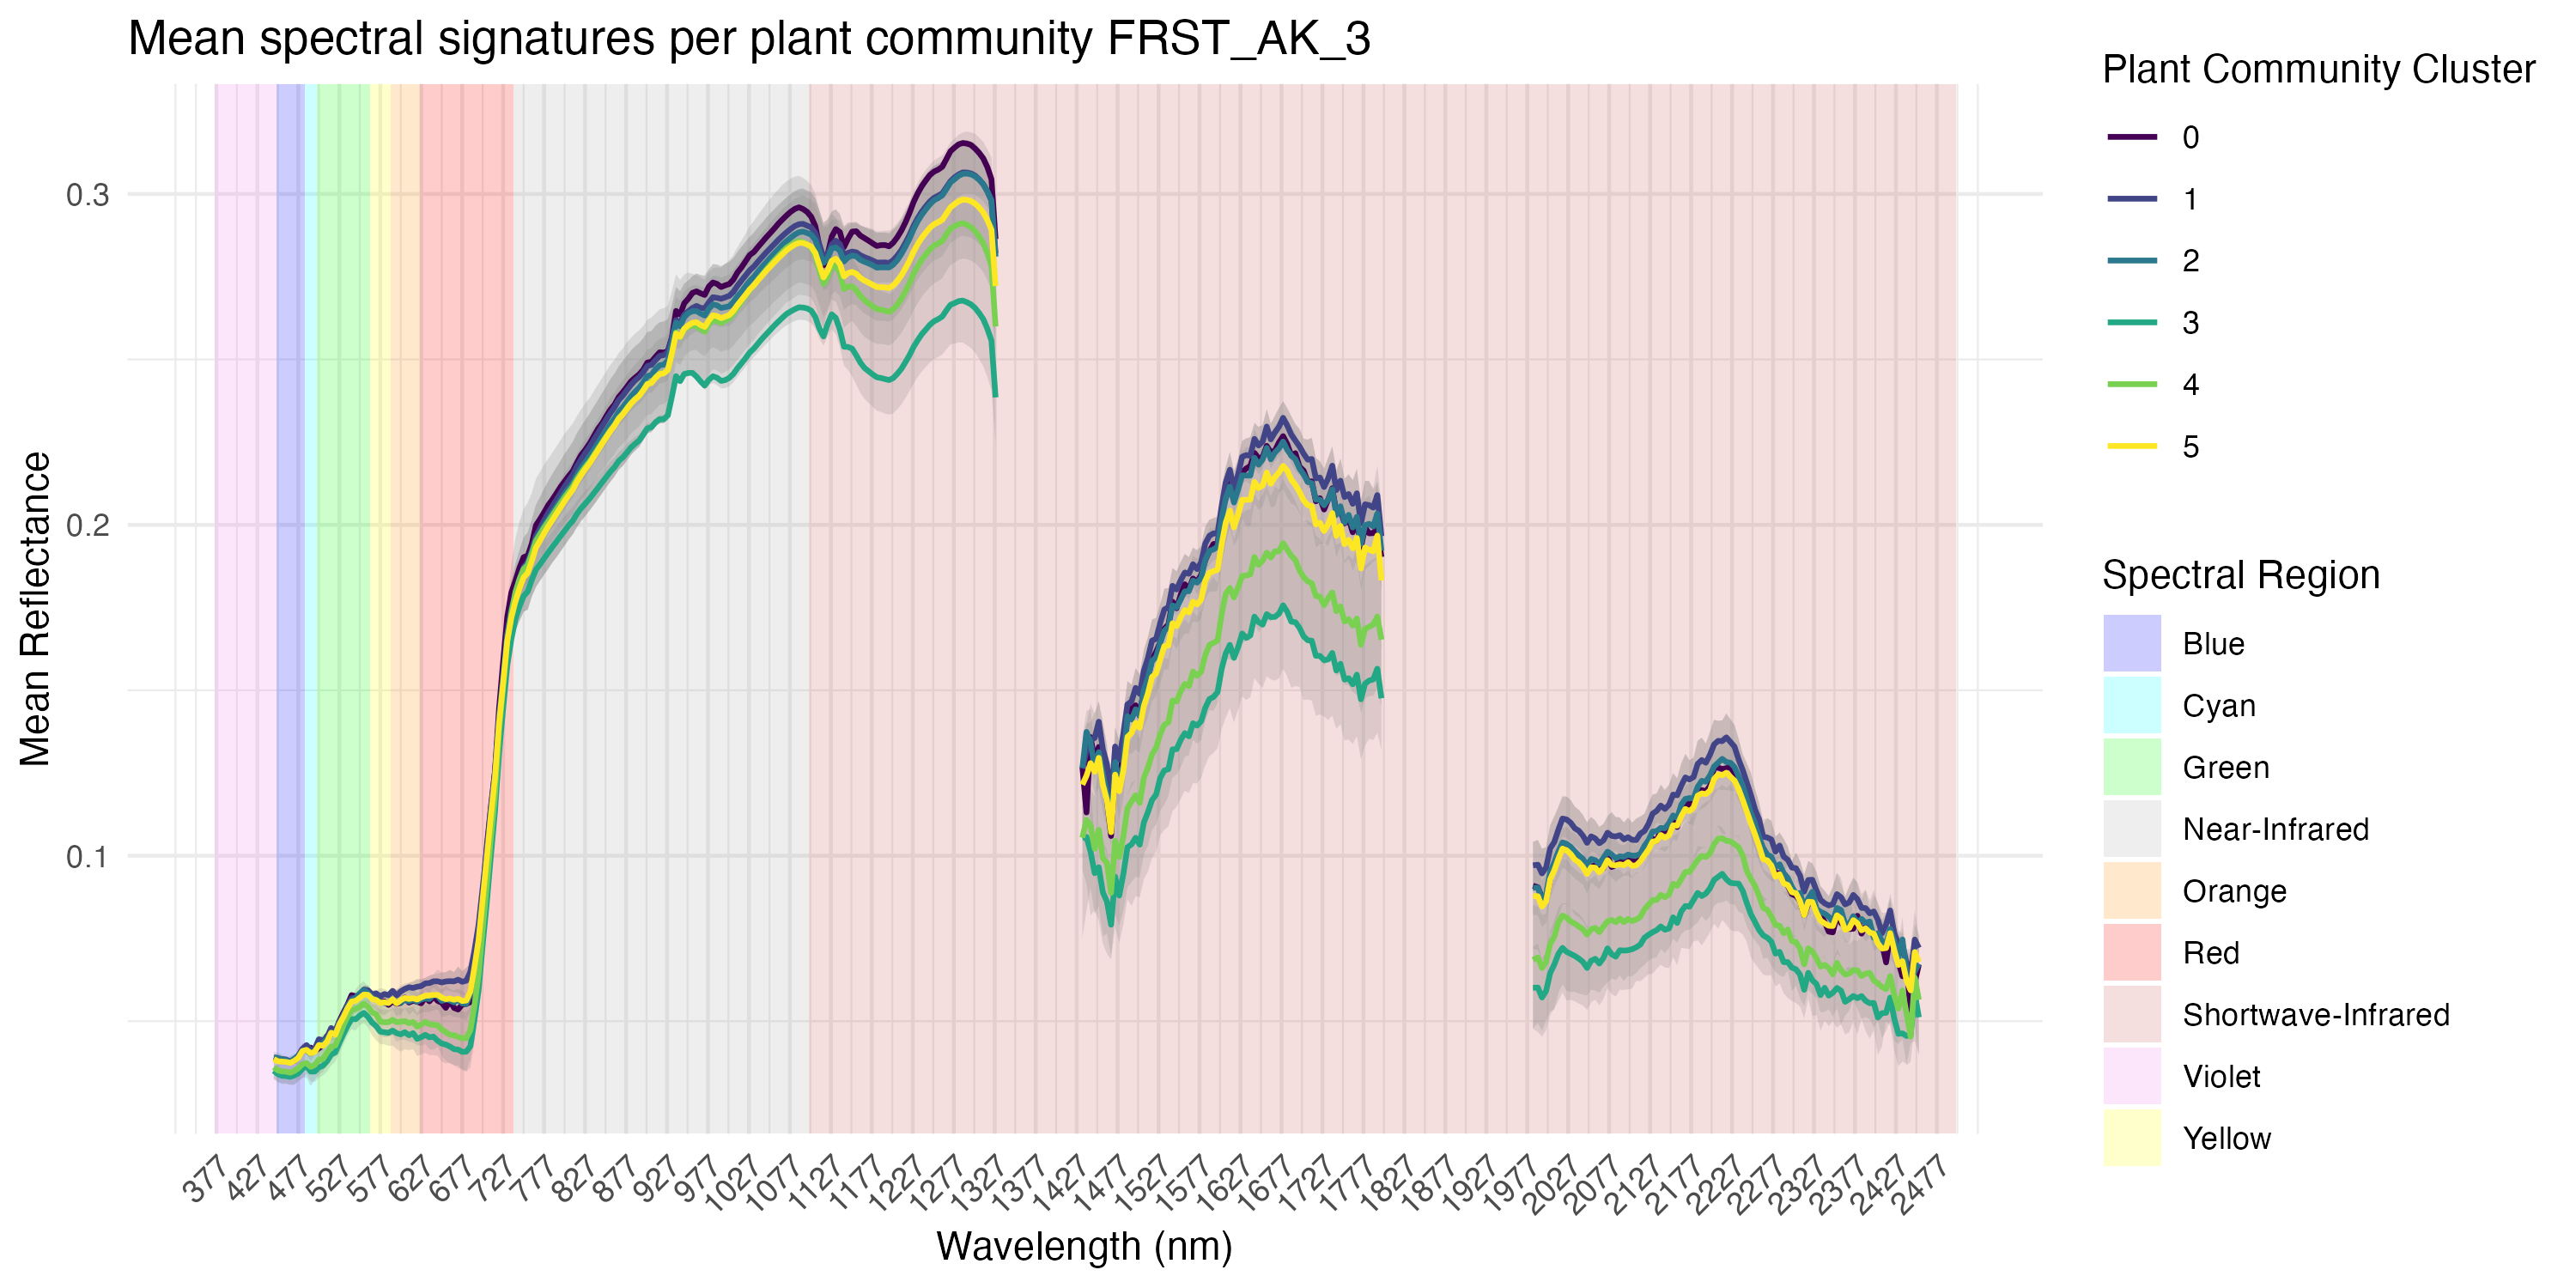
\includegraphics[width=\textwidth]{Figures/spectral_signatures/FRST_AK_3_mean_signature_plot_plant_community.png}
    \caption{}
    \label{fig:mss_pc_frstak3}
  \end{subfigure}

  \caption{Spectral signature plot \ref{fig:ss_pc_frstak3} and mean spectral signature plot \ref{fig:mss_pc_frstak3} grouped by plant community cluster for test site FRST\_AK\_3}
  \label{fig:group_pc_ht_frstak3}
\end{figure}

\subsection{PRUAIR\_DW\_1}

\begin{figure}[H]
  \centering

  \begin{subfigure}[b]{0.49\textwidth}
    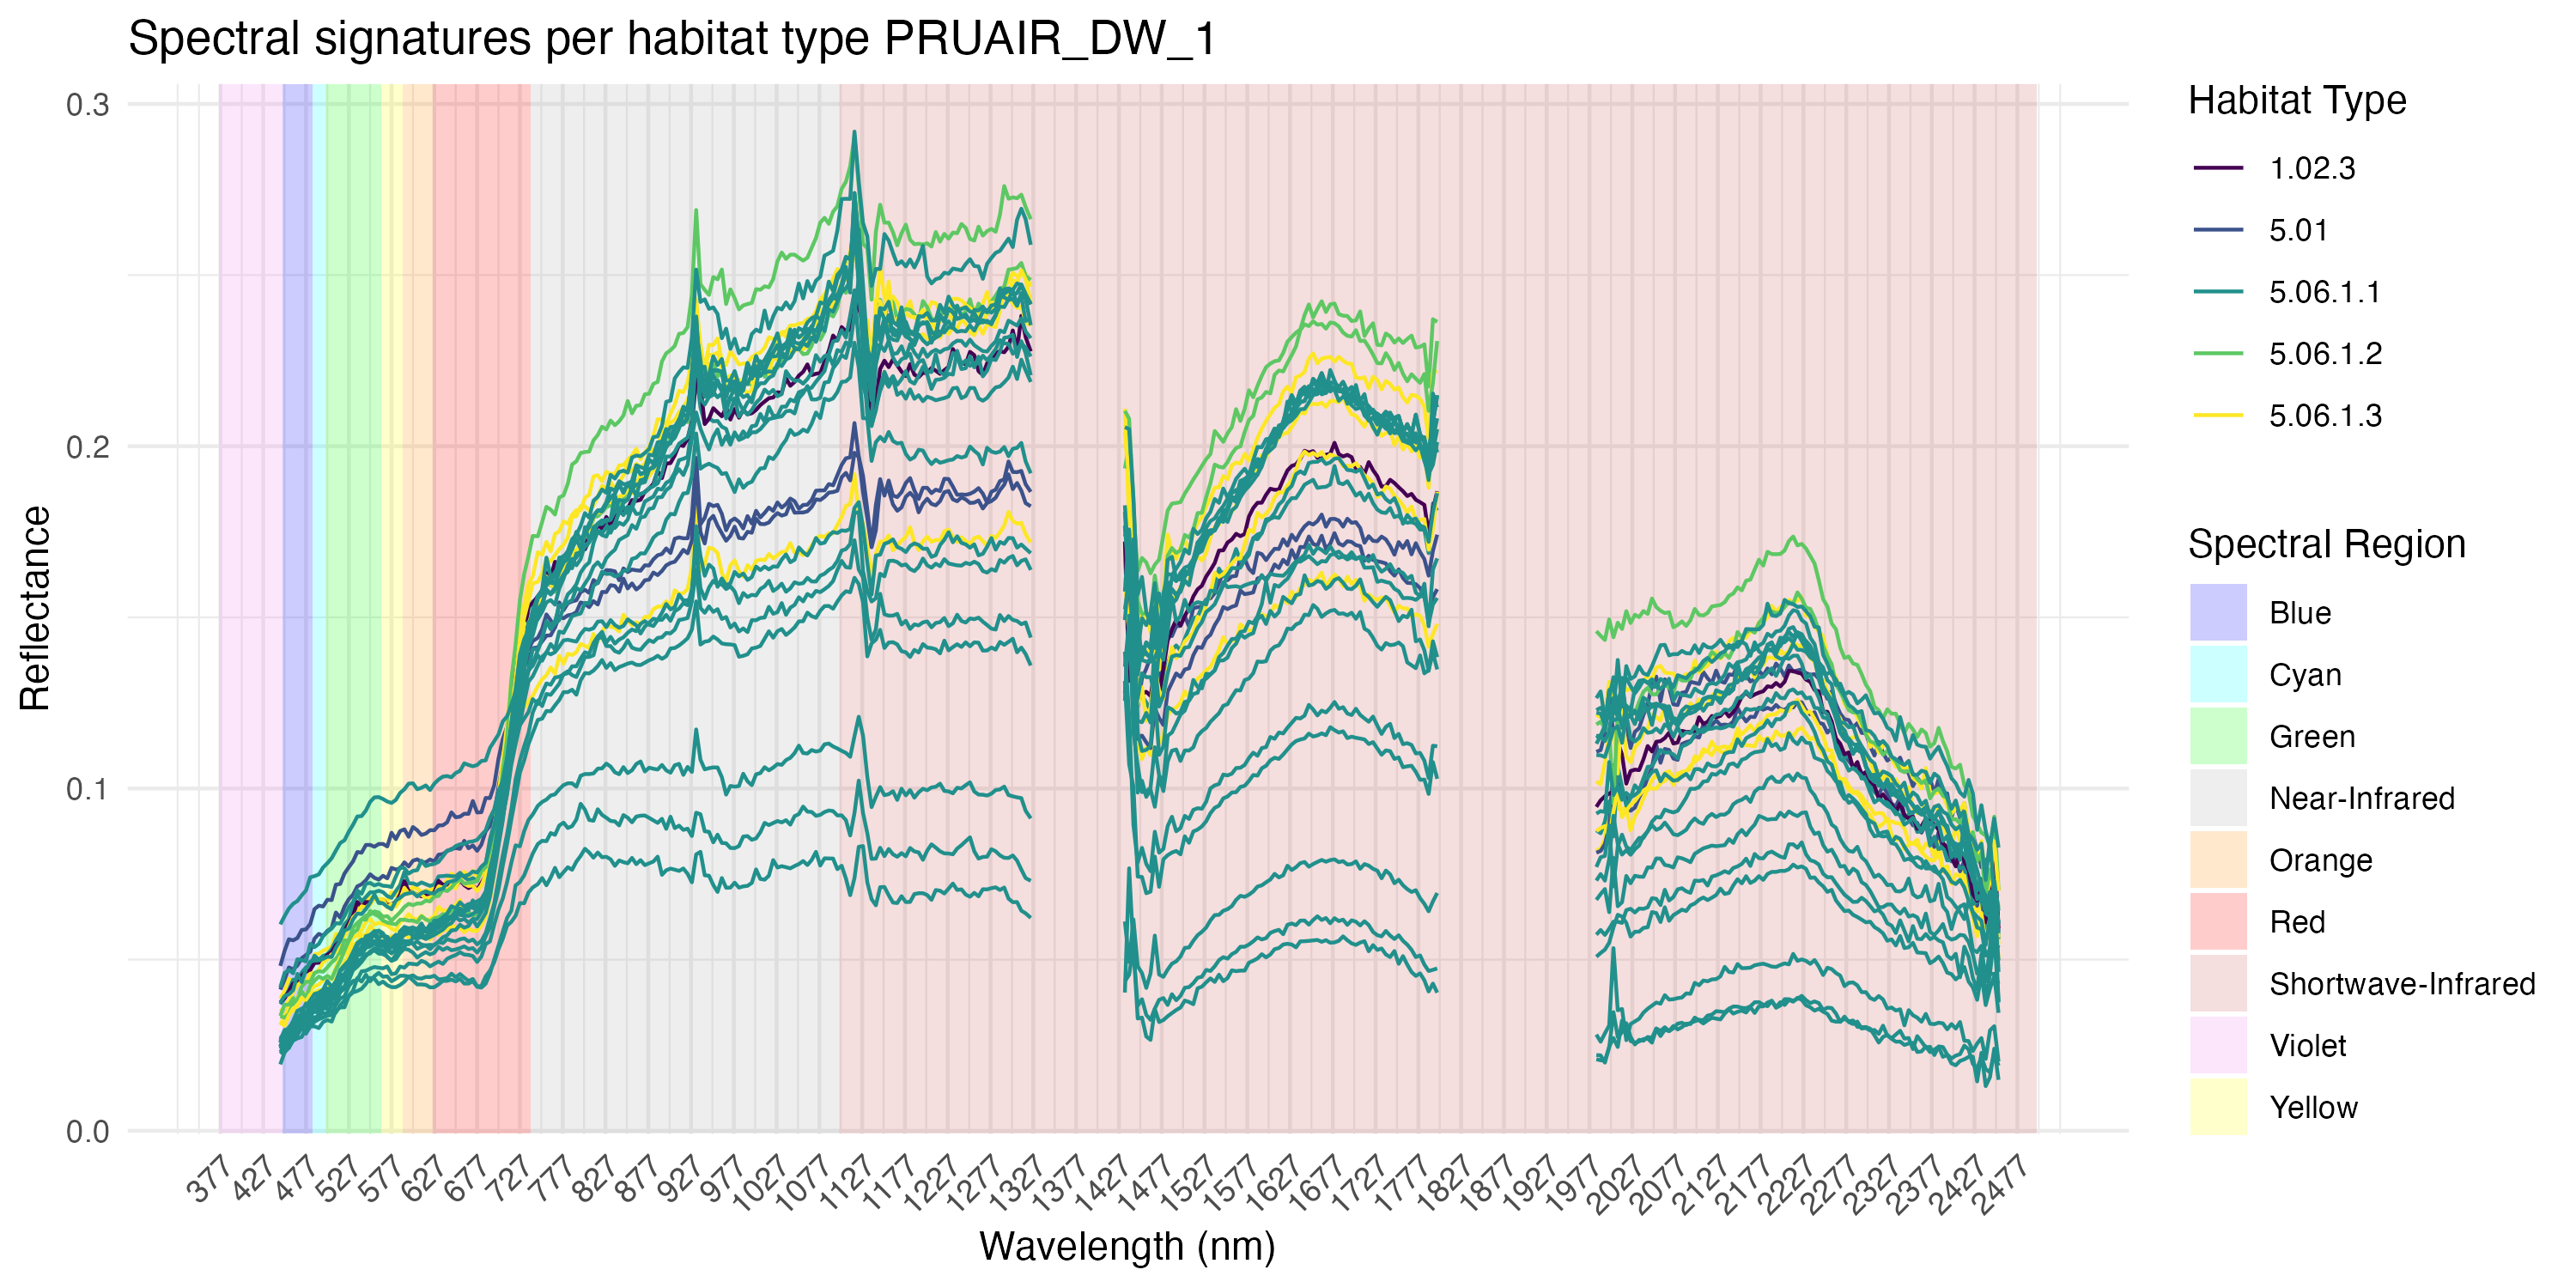
\includegraphics[width=\textwidth]{Figures/spectral_signatures/PRUAIR_DW_1_signature_plot_habitat.png}
    \caption{}
    \label{fig:ss_ht_pruairdw1}
  \end{subfigure}
  \hfill
  \begin{subfigure}[b]{0.49\textwidth}
    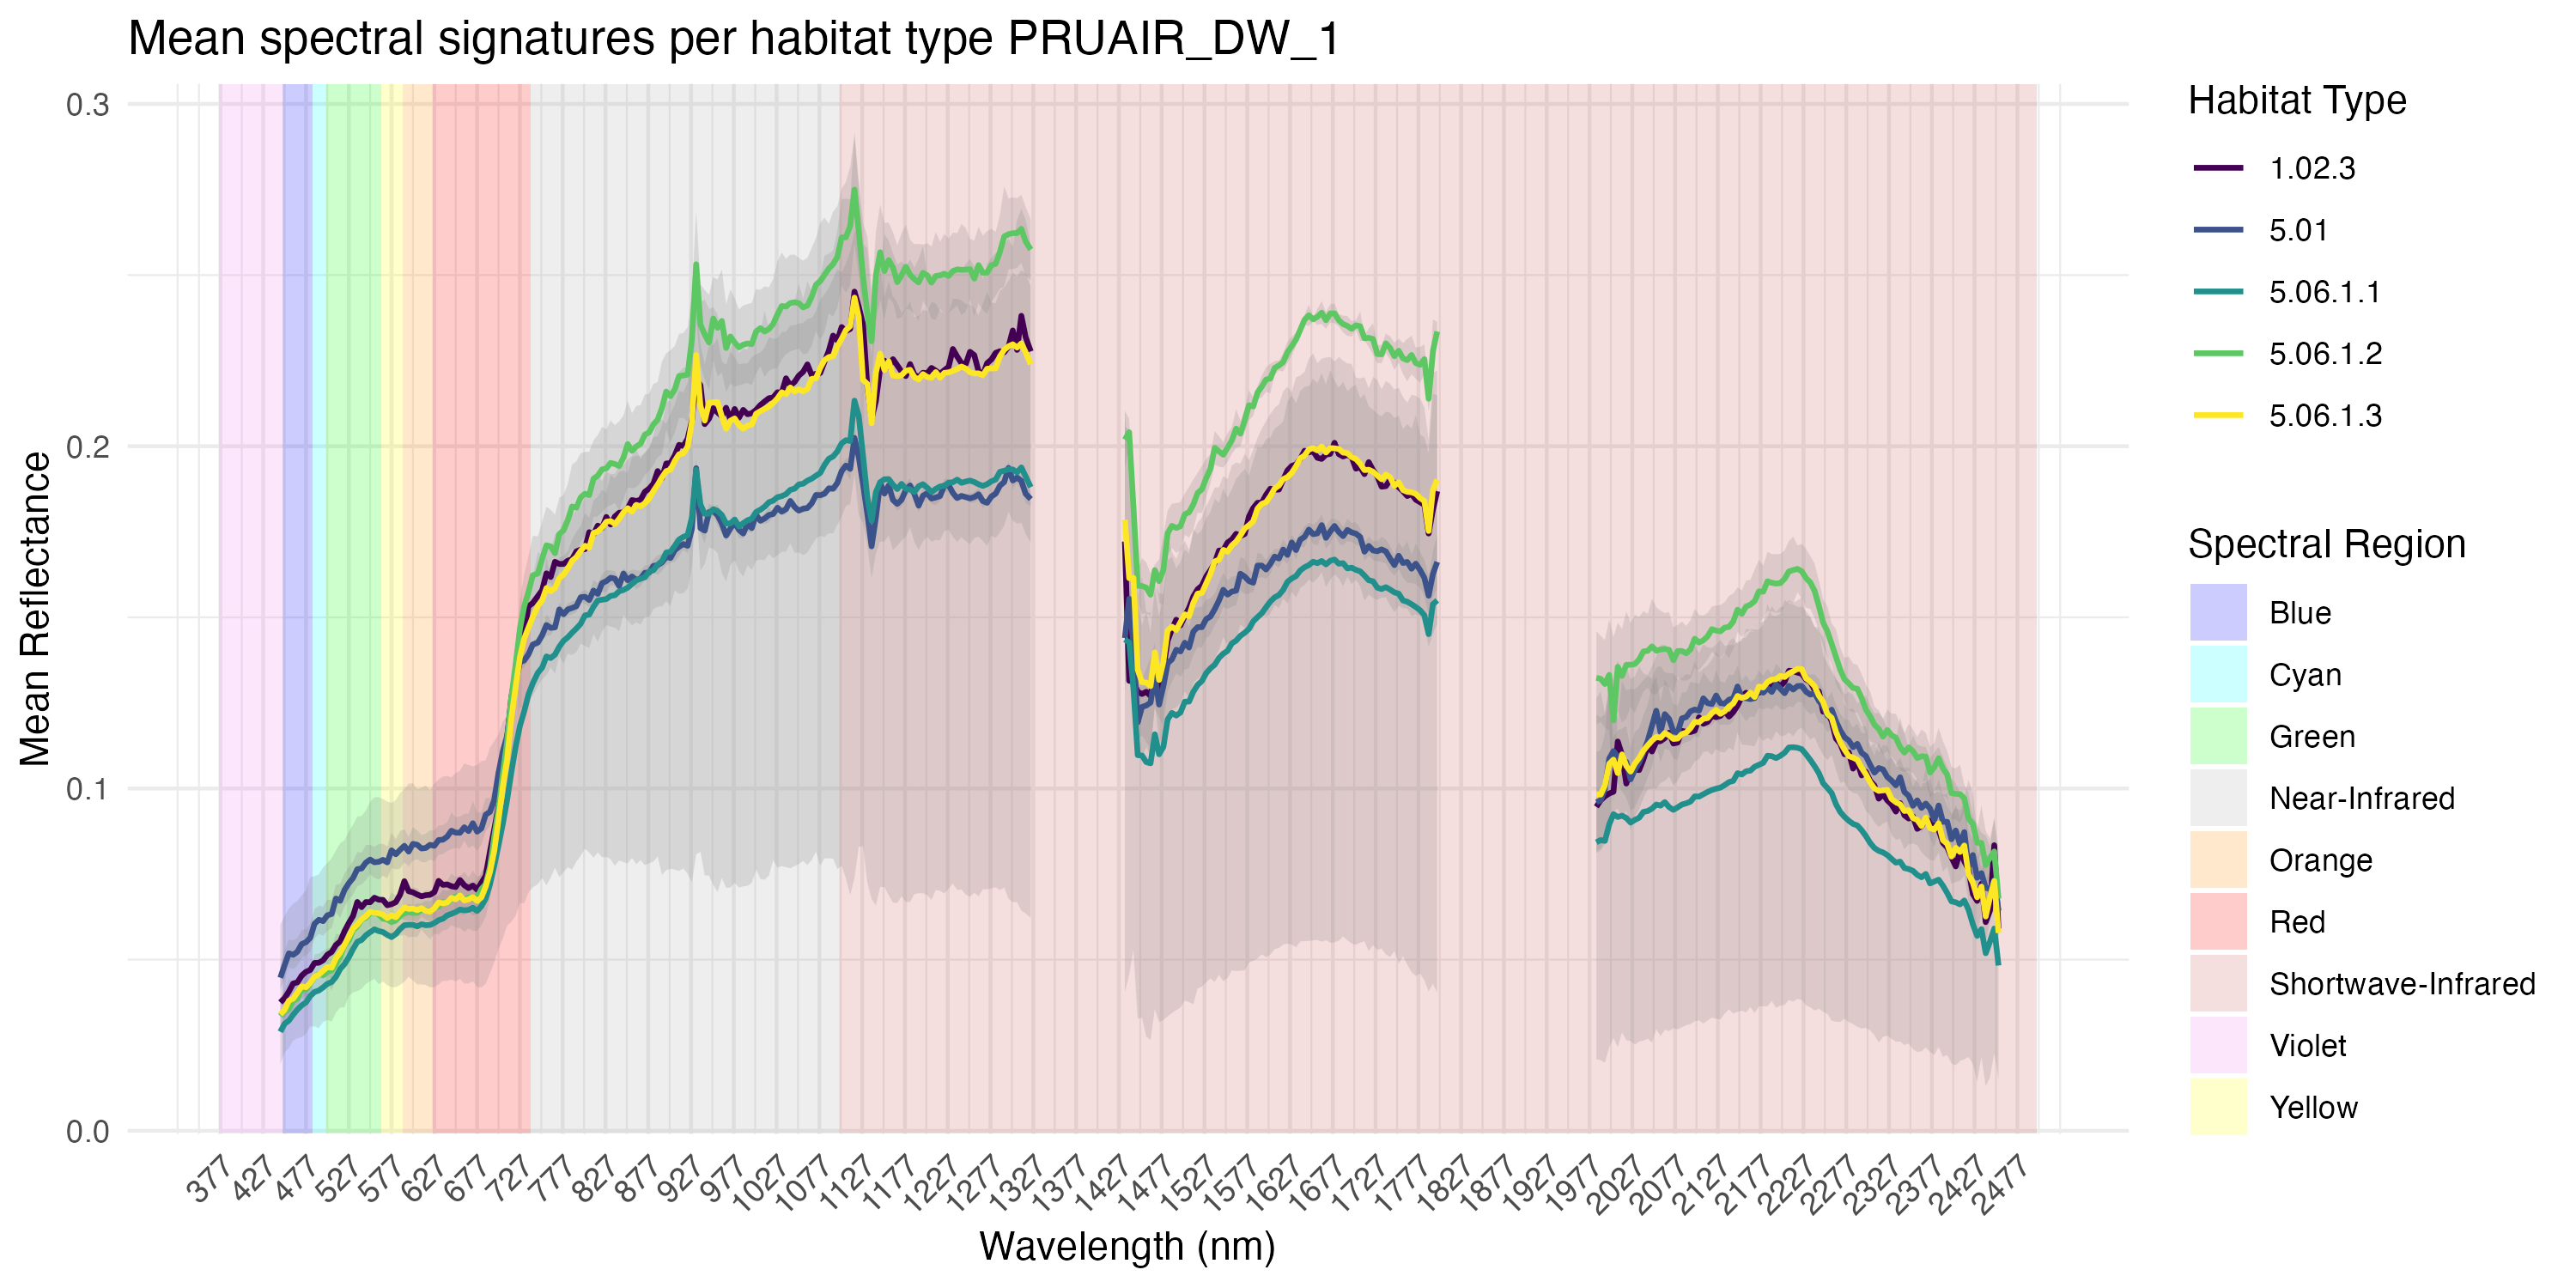
\includegraphics[width=\textwidth]{Figures/spectral_signatures/PRUAIR_DW_1_mean_signature_plot_habitat.png}
    \caption{}
    \label{fig:mss_ht_pruairdw1}
  \end{subfigure}

  \caption{Spectral signature plot \ref{fig:ss_ht_pruairdw1} and mean spectral signature plot \ref{fig:mss_ht_pruairdw1} grouped by habitat type for test site PRUAIR\_DW\_1}
  \label{fig:group_ss_ht_pruairdw1}
\end{figure}

\begin{figure}[H]
  \centering

  \begin{subfigure}[b]{0.49\textwidth}
    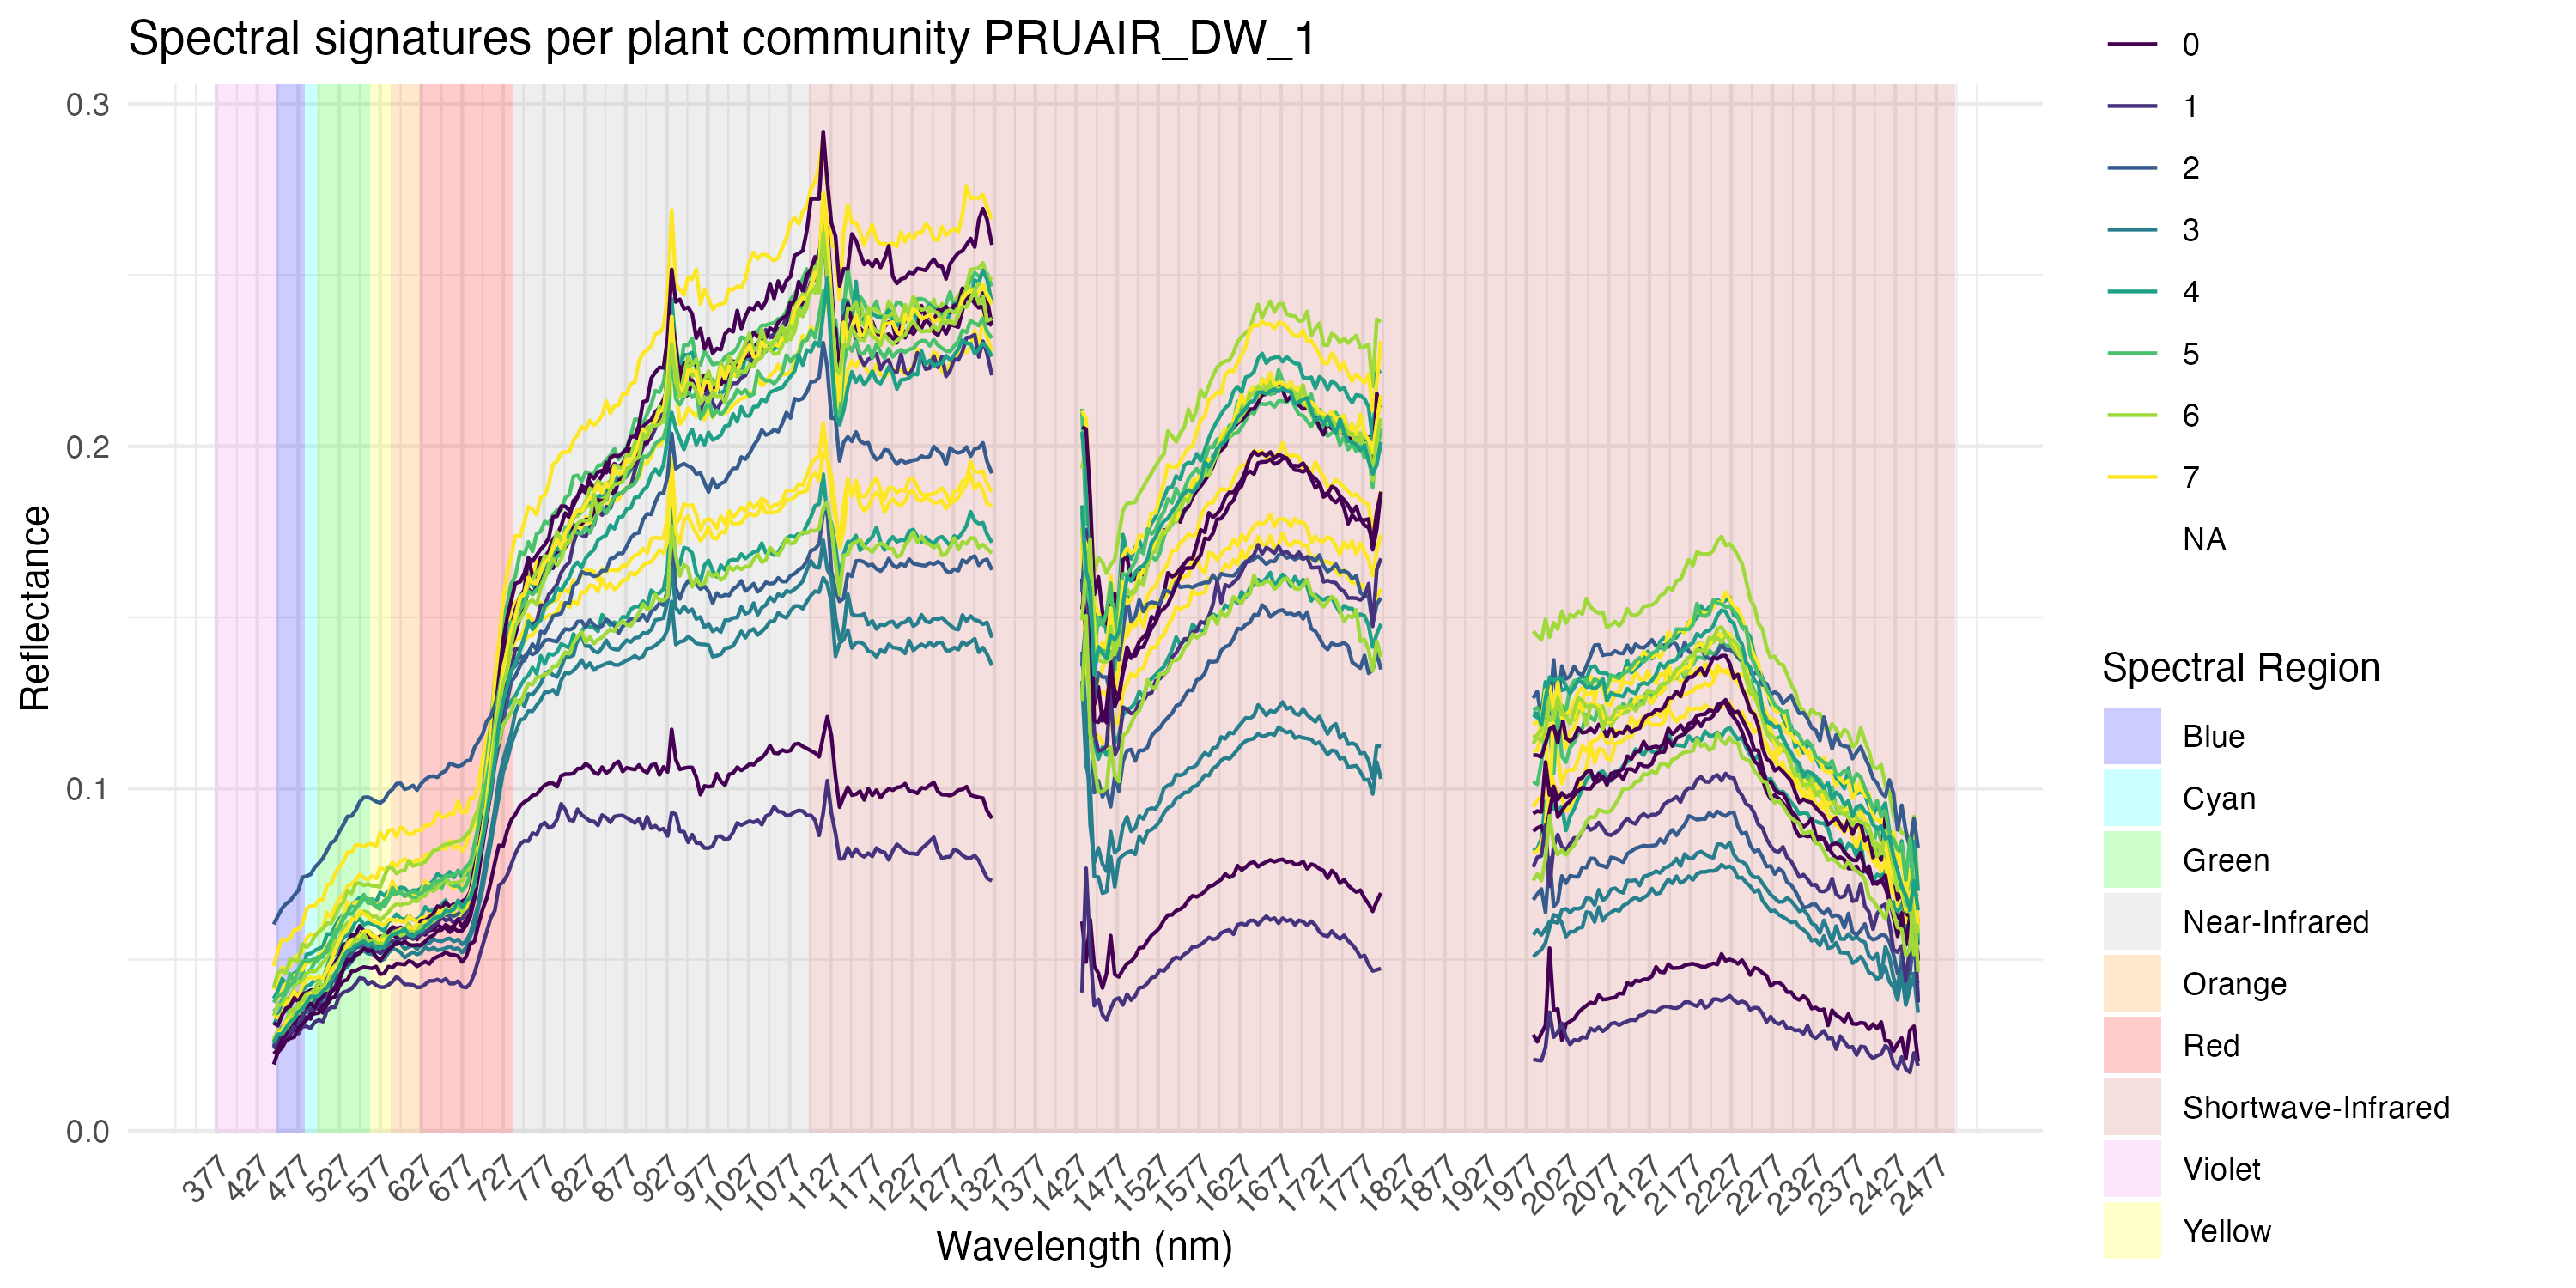
\includegraphics[width=\textwidth]{Figures/spectral_signatures/PRUAIR_DW_1_signature_plot_plant_community.png}
    \caption{}
    \label{fig:ss_pc_pruairdw1}
  \end{subfigure}
  \hfill
  \begin{subfigure}[b]{0.49\textwidth}
    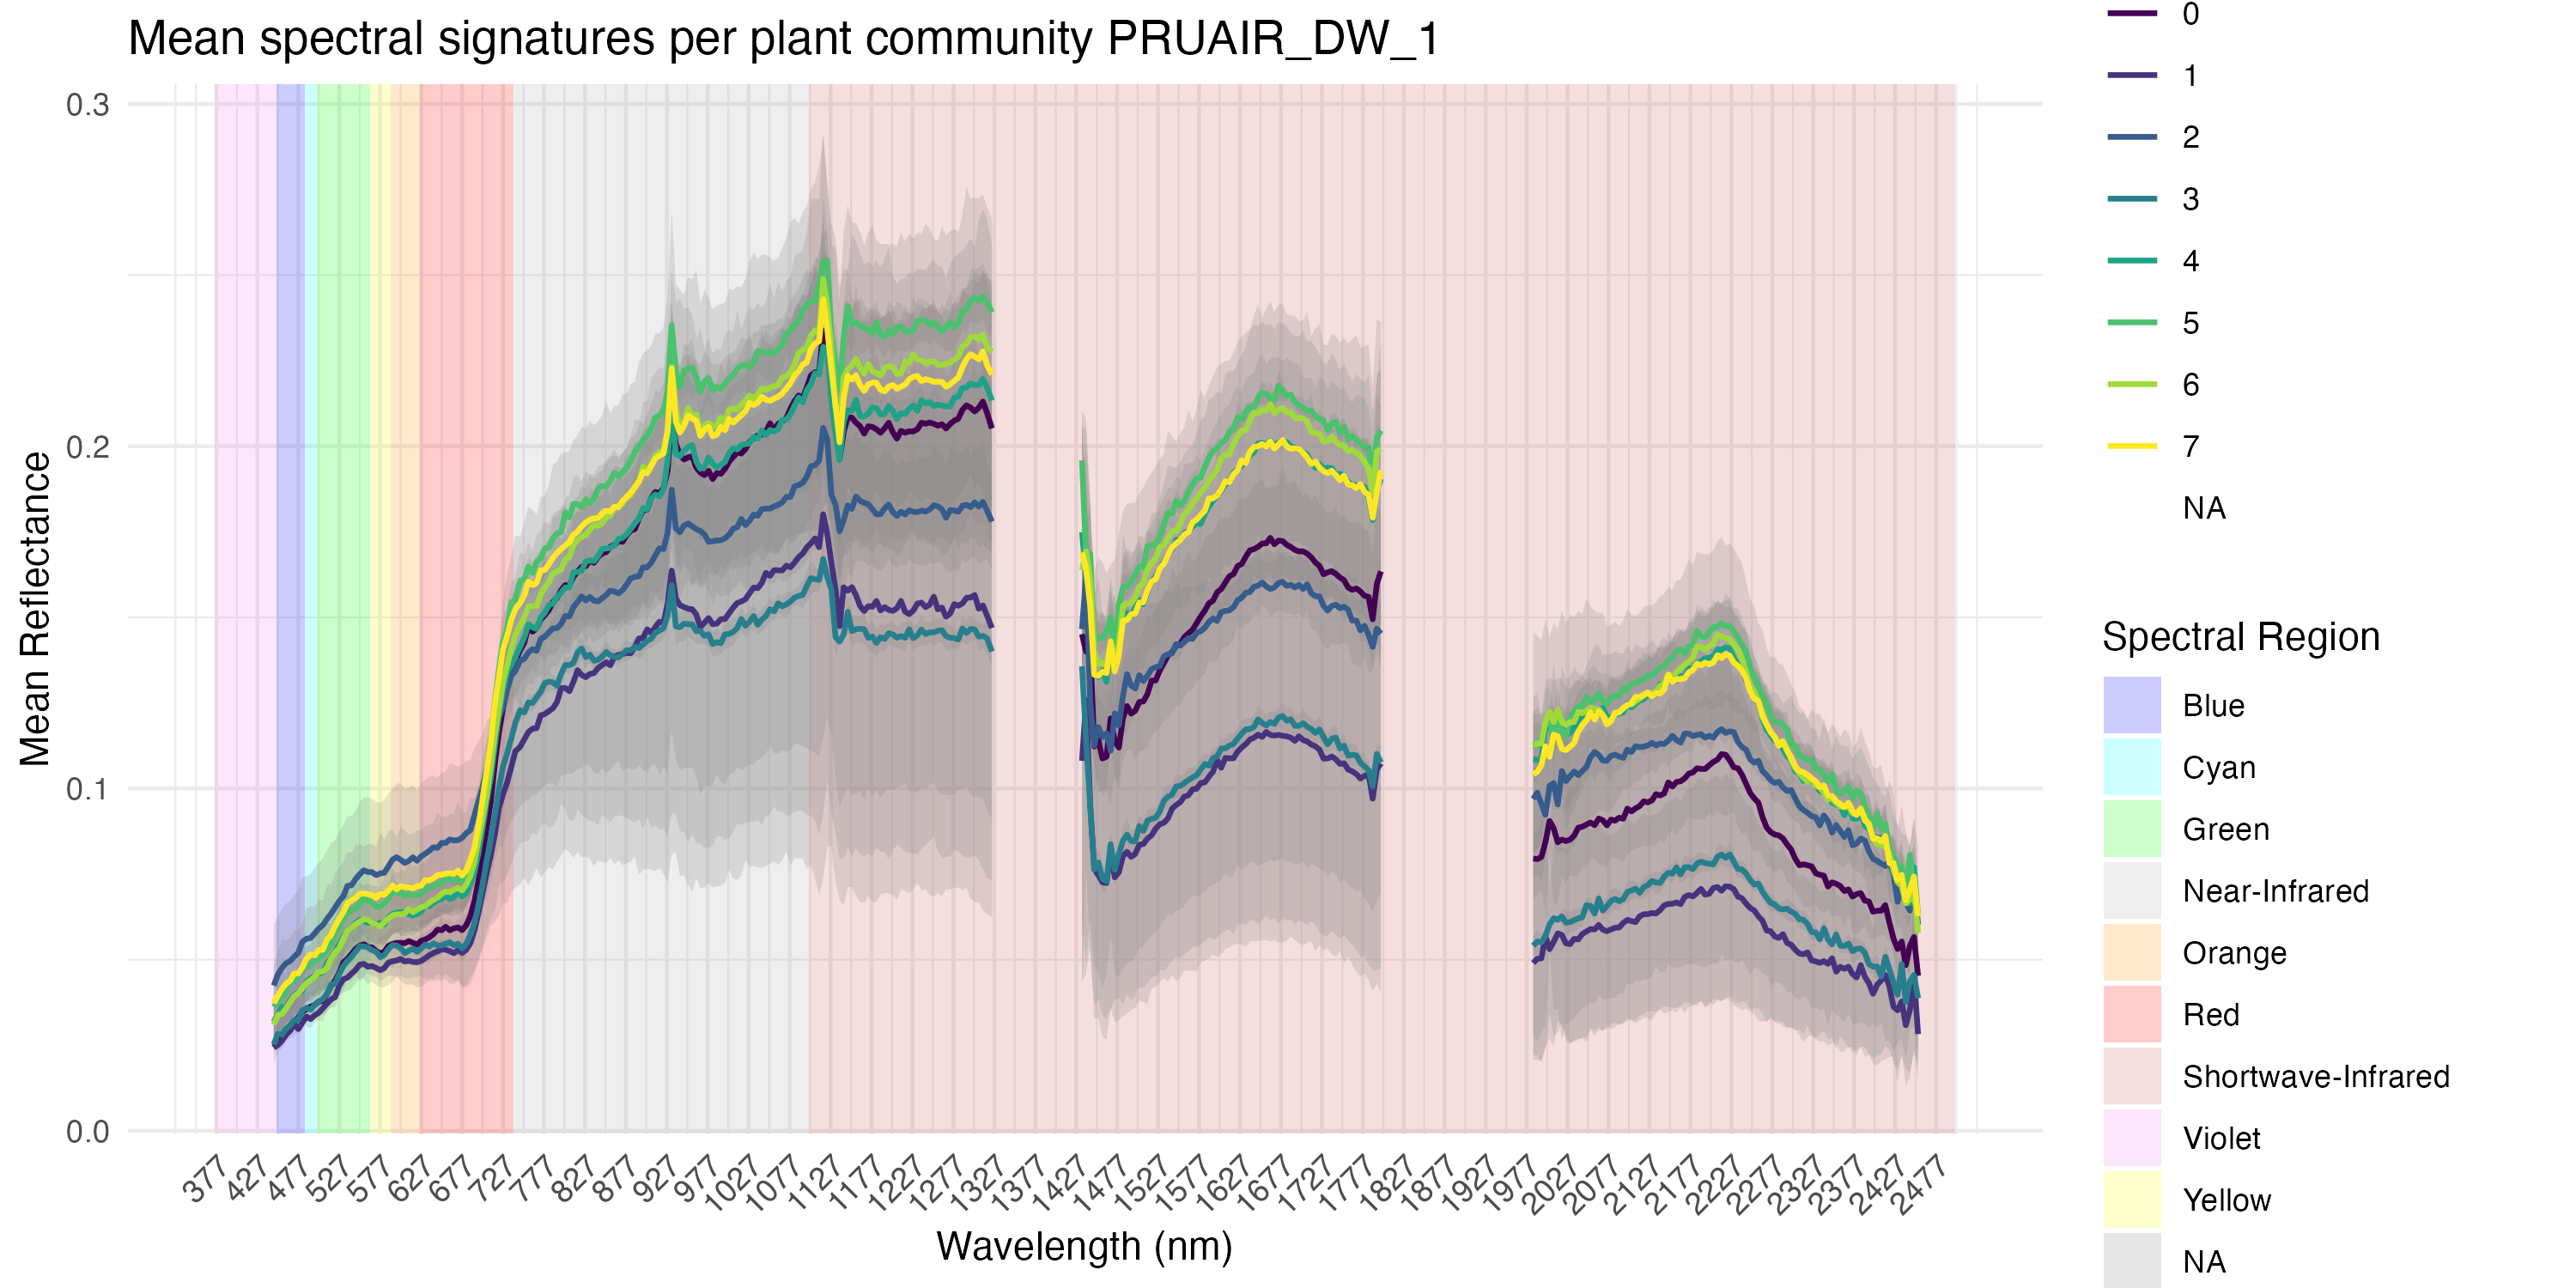
\includegraphics[width=\textwidth]{Figures/spectral_signatures/PRUAIR_DW_1_mean_signature_plot_plant_community.png}
    \caption{}
    \label{fig:mss_pc_pruairdw1}
  \end{subfigure}

  \caption{Spectral signature plot \ref{fig:ss_pc_pruairdw1} and mean spectral signature plot \ref{fig:mss_pc_pruairdw1} grouped by plant community cluster for test site PRUAIR\_DW\_1}
  \label{fig:group_pc_ht_pruairdw1}
\end{figure}

\subsection{PRUARC\_DW\_1}

\begin{figure}[H]
  \centering

  \begin{subfigure}[b]{0.49\textwidth}
    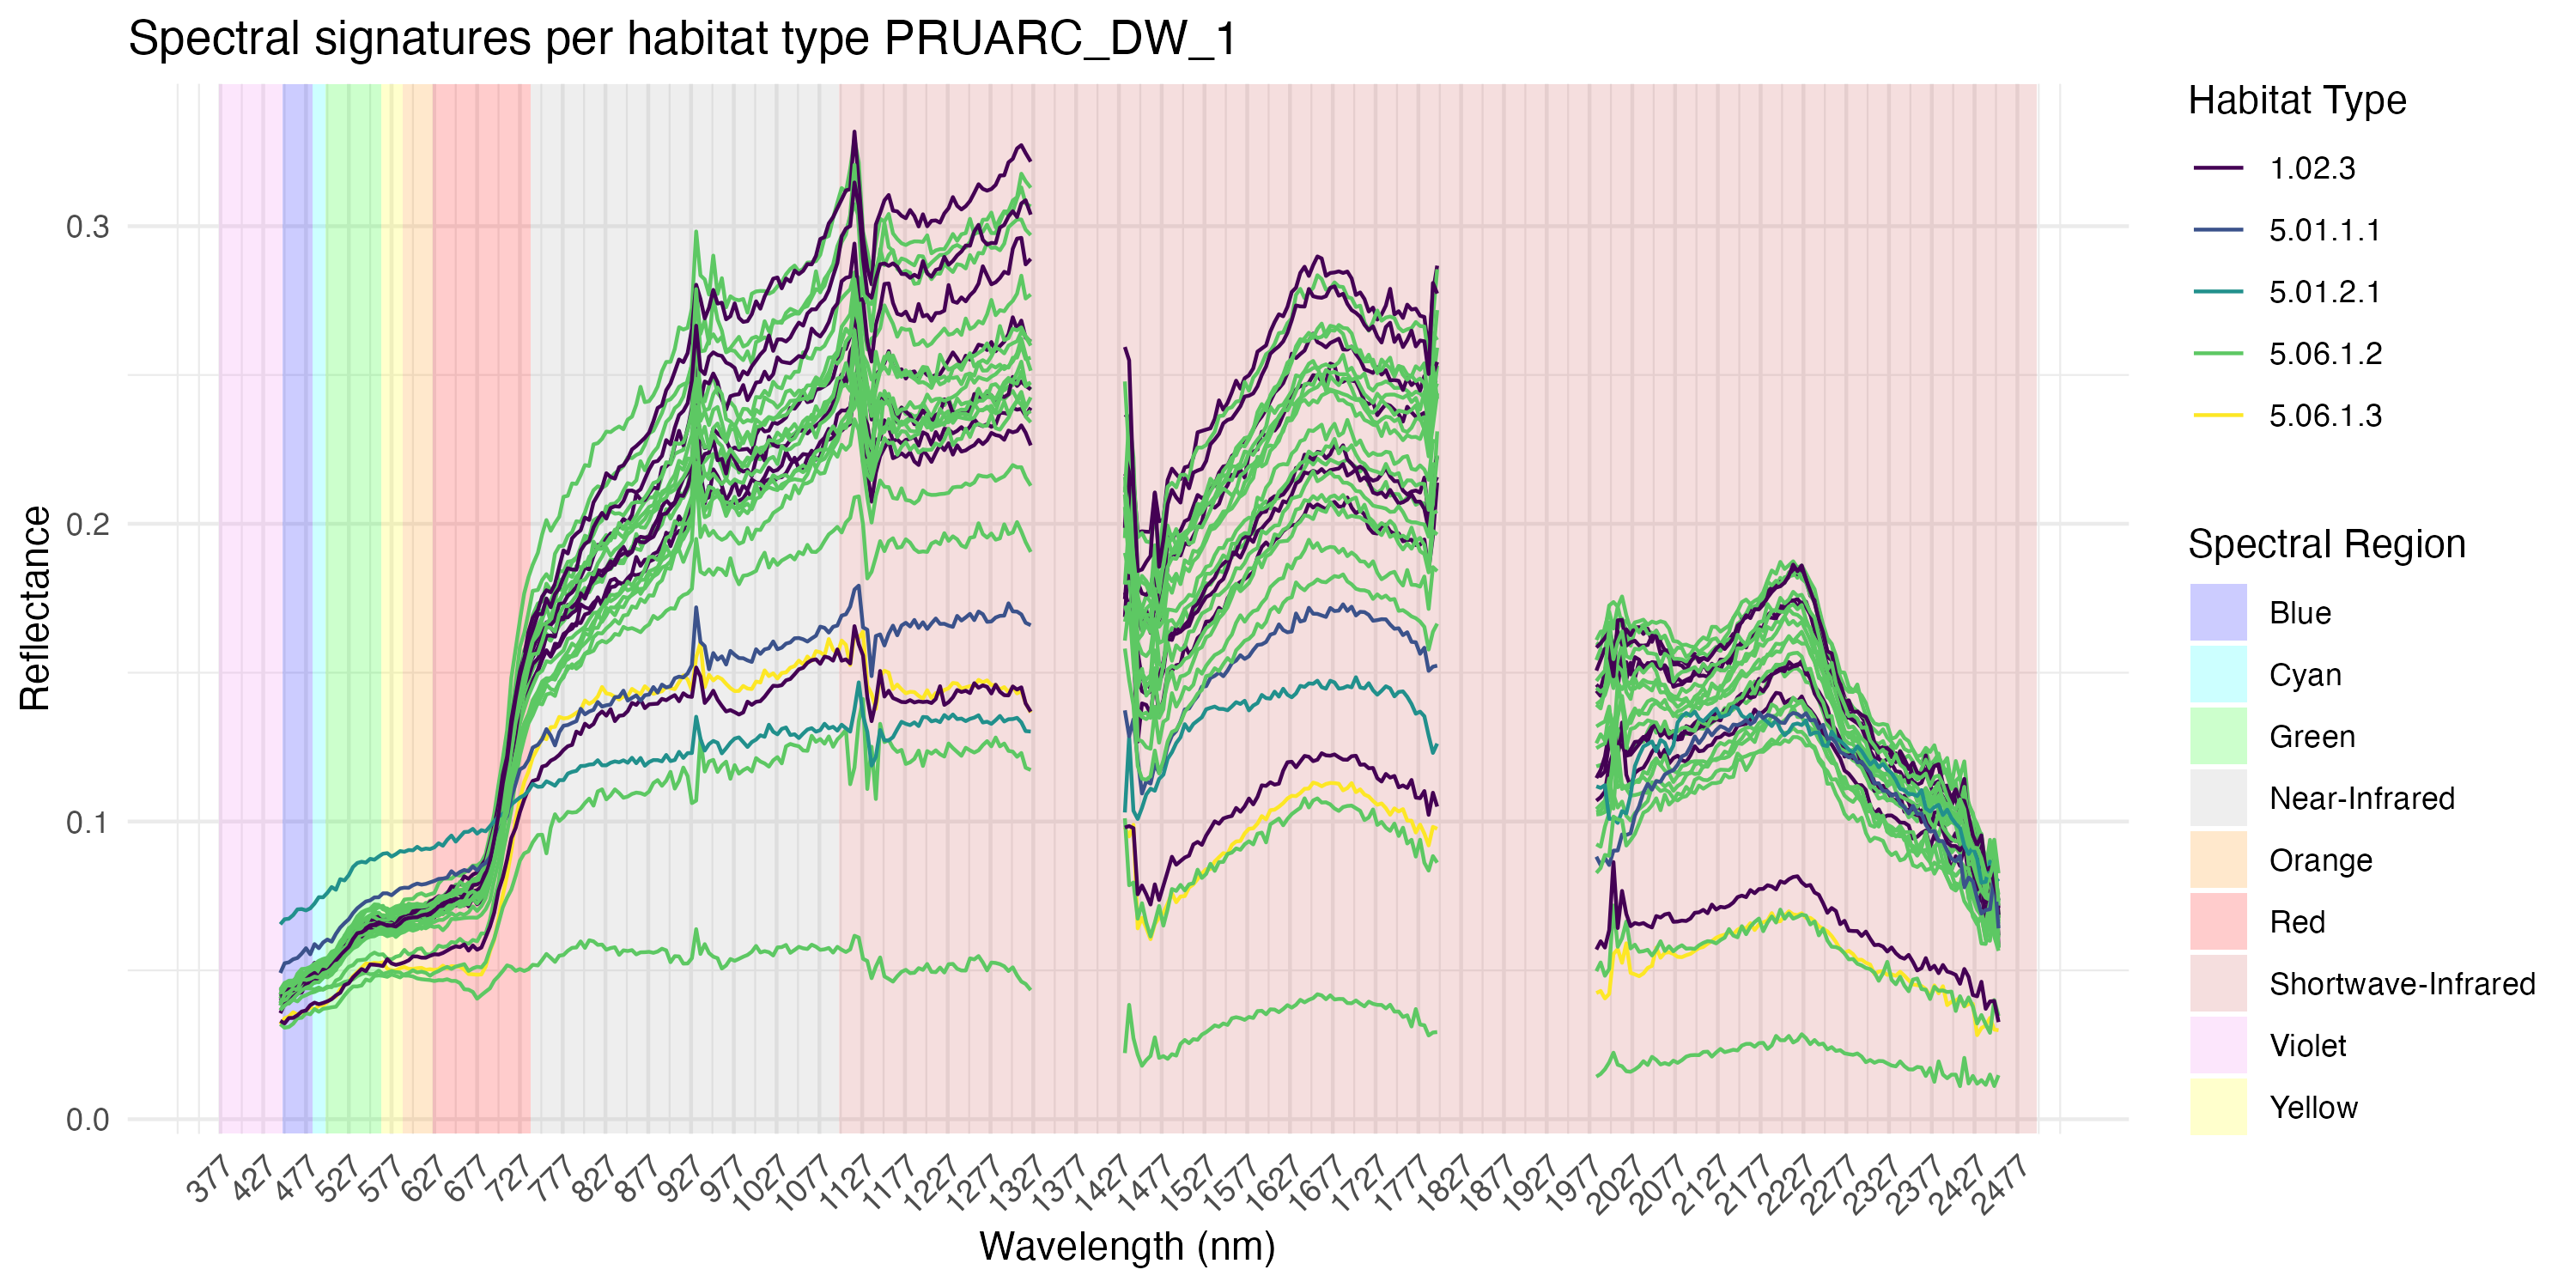
\includegraphics[width=\textwidth]{Figures/spectral_signatures/PRUARC_DW_1_signature_plot_habitat.png}
    \caption{}
    \label{fig:ss_ht_pruarcdw1}
  \end{subfigure}
  \hfill
  \begin{subfigure}[b]{0.49\textwidth}
    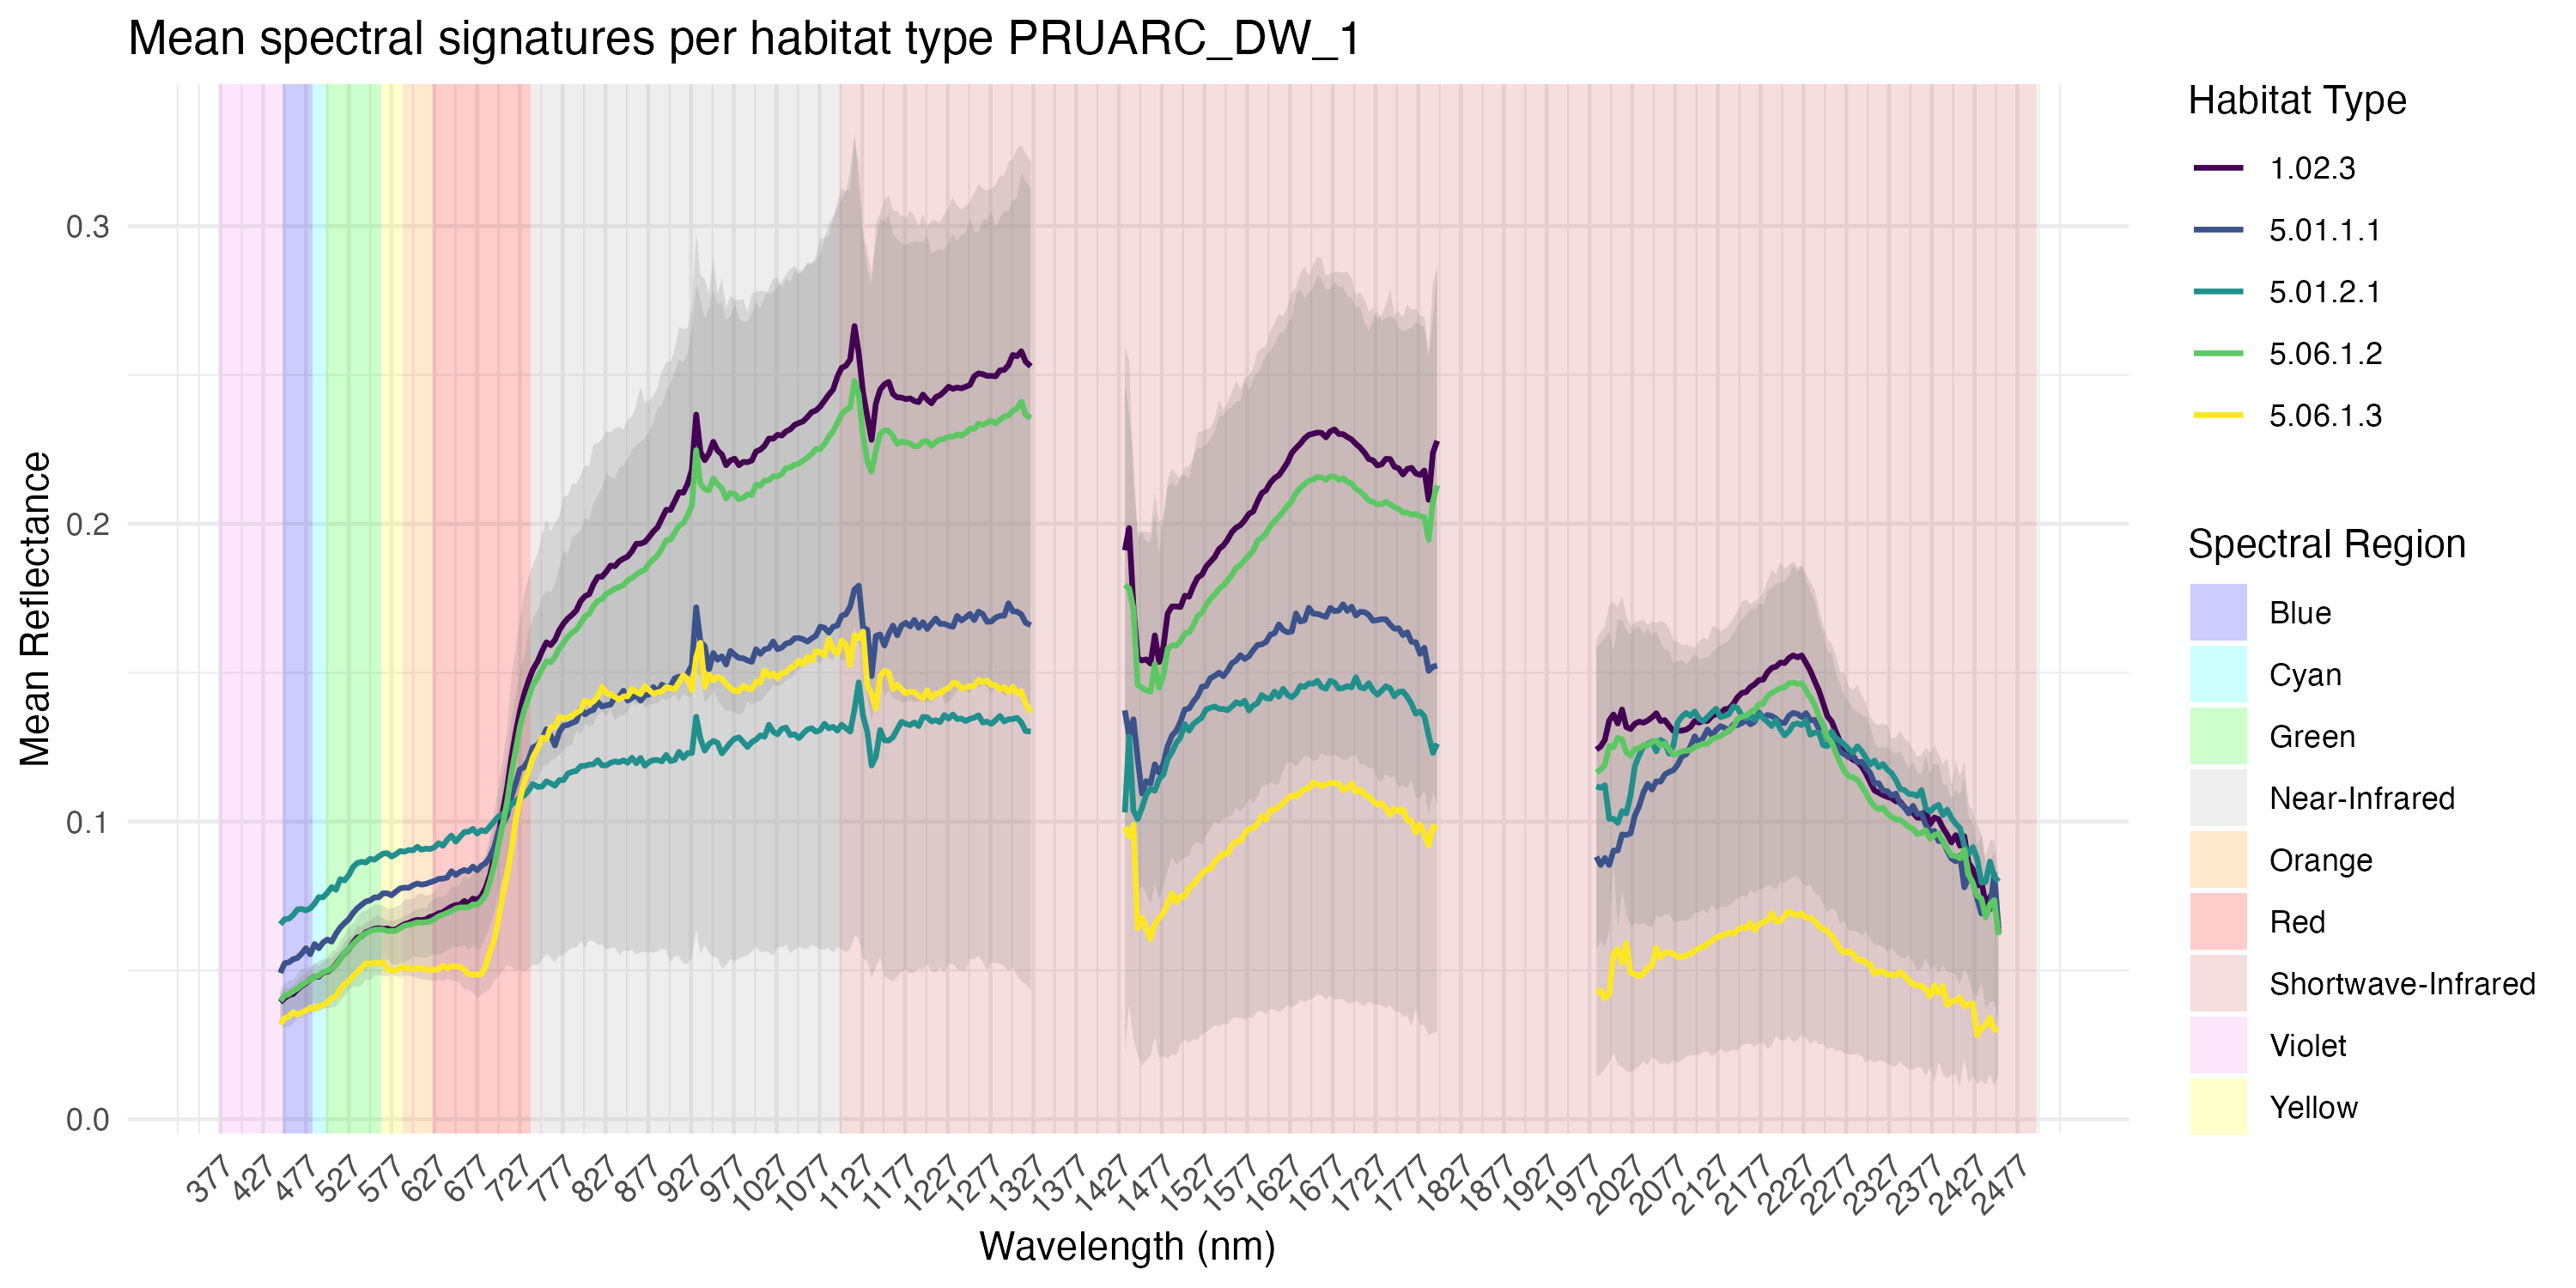
\includegraphics[width=\textwidth]{Figures/spectral_signatures/PRUARC_DW_1_mean_signature_plot_habitat.png}
    \caption{}
    \label{fig:mss_ht_pruarcdw1}
  \end{subfigure}

  \caption{Spectral signature plot \ref{fig:ss_ht_pruarcdw1} and mean spectral signature plot \ref{fig:mss_ht_pruarcdw1} grouped by habitat type for test site PRUARC\_DW\_1}
  \label{fig:group_ss_ht_pruarcdw1}
\end{figure}

\begin{figure}[H]
  \centering

  \begin{subfigure}[b]{0.49\textwidth}
    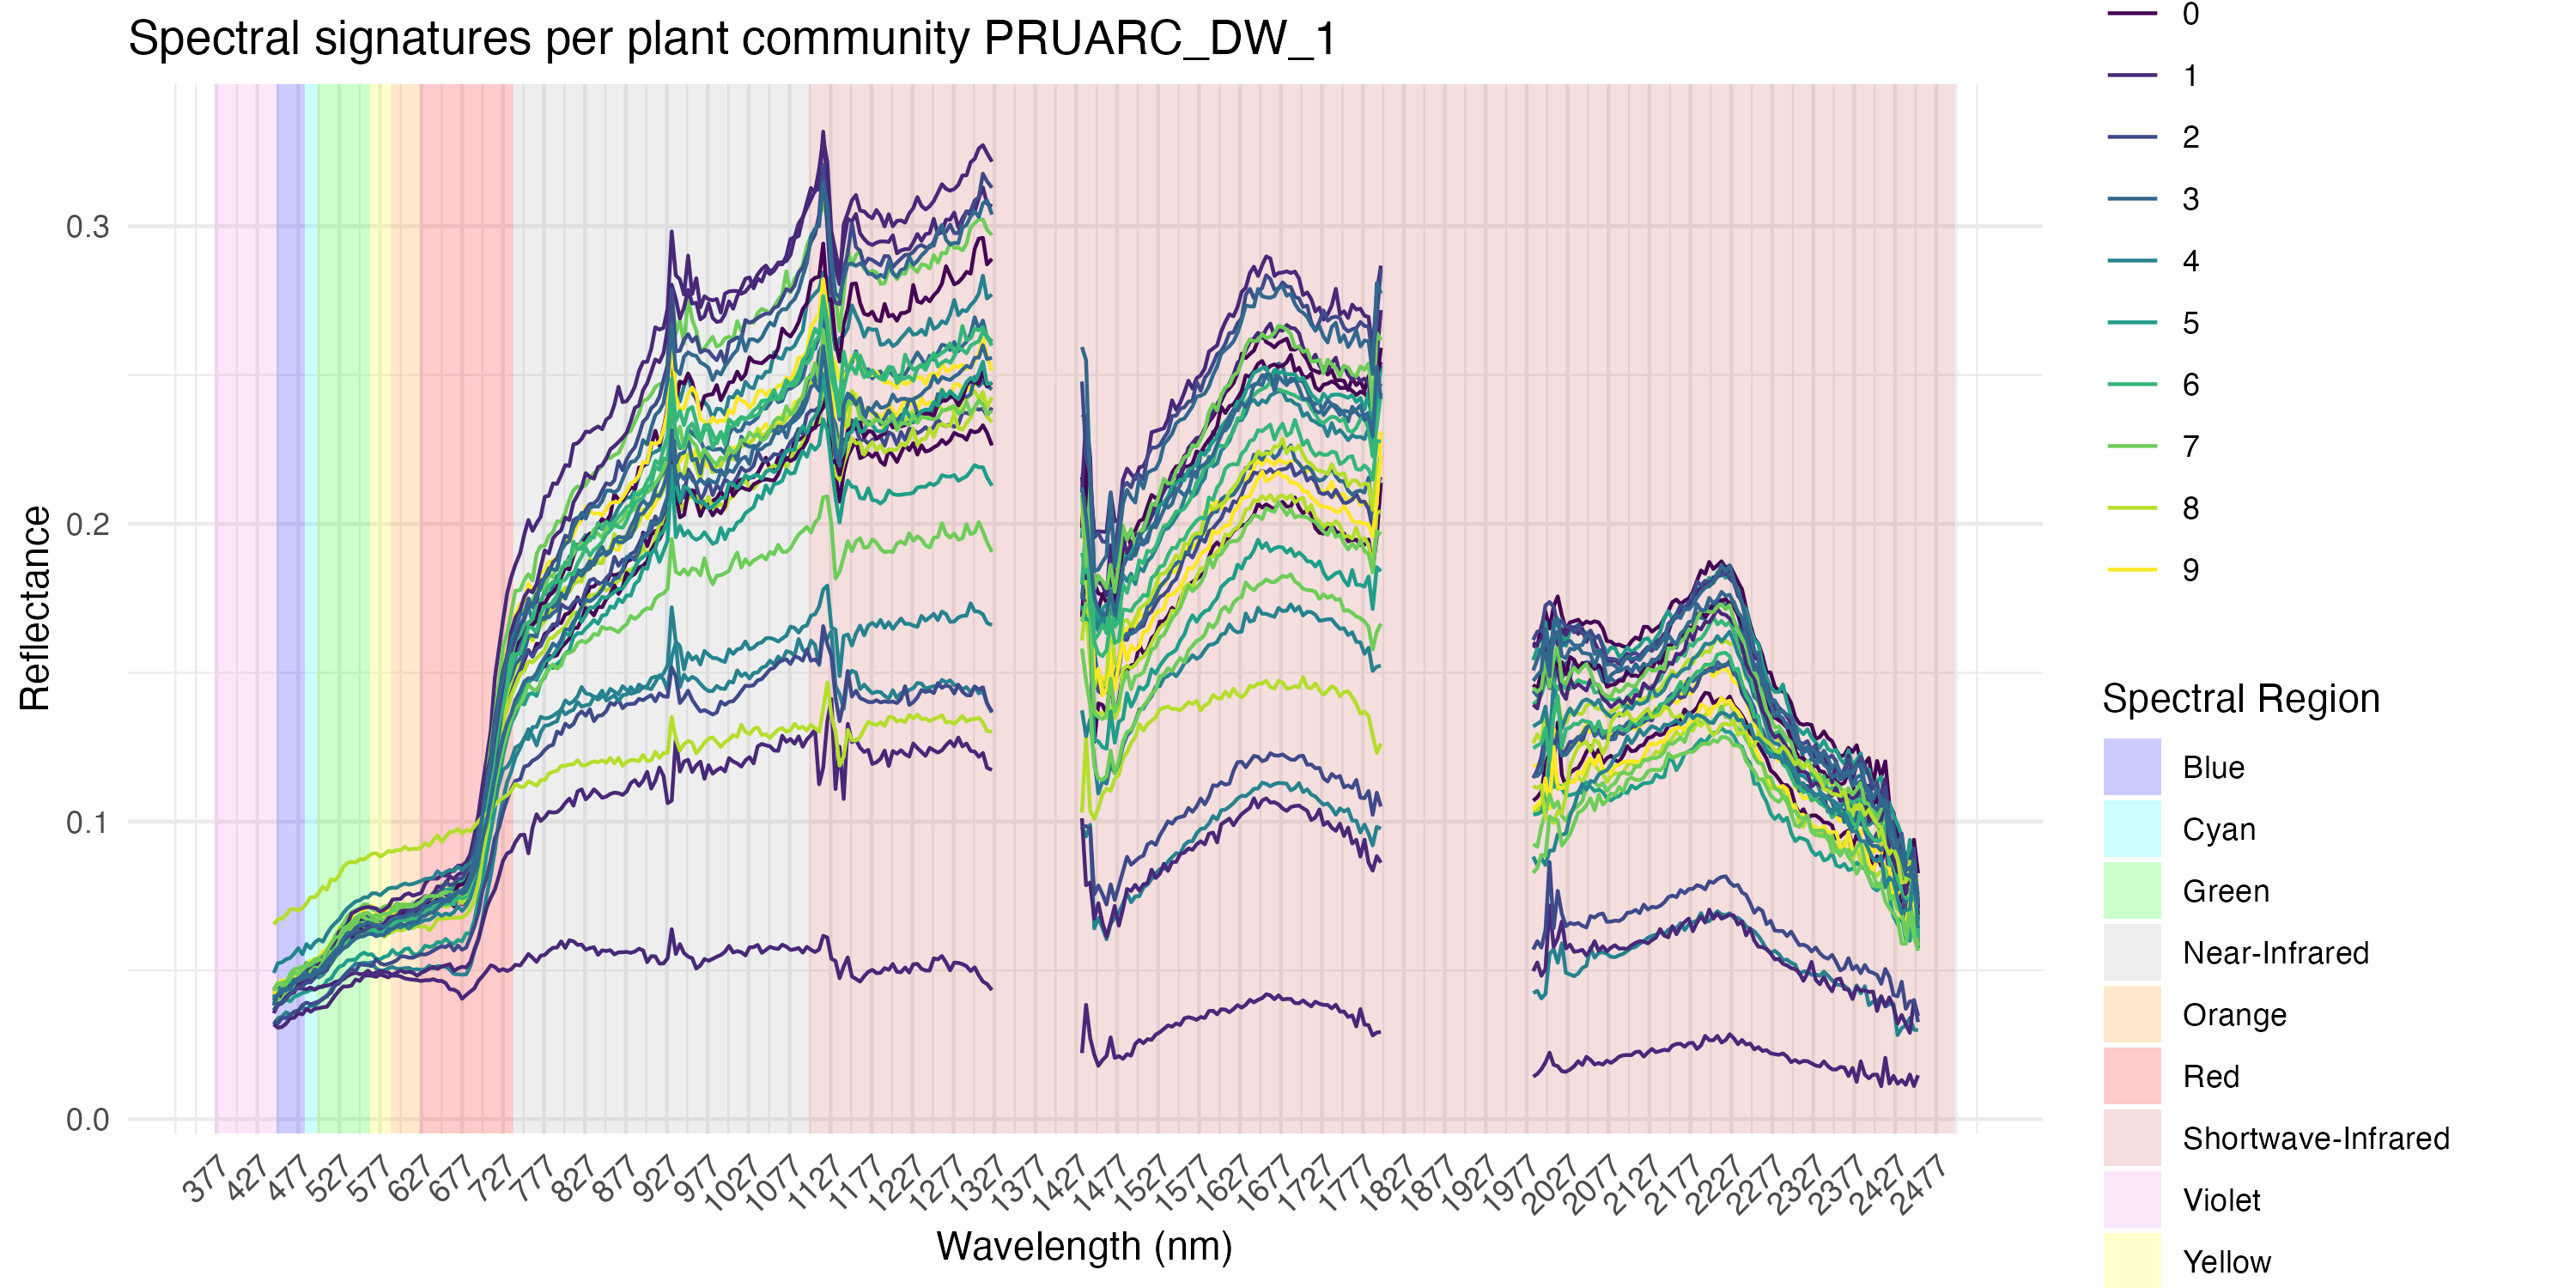
\includegraphics[width=\textwidth]{Figures/spectral_signatures/PRUARC_DW_1_signature_plot_plant_community.png}
    \caption{}
    \label{fig:ss_pc_pruarcdw1}
  \end{subfigure}
  \hfill
  \begin{subfigure}[b]{0.49\textwidth}
    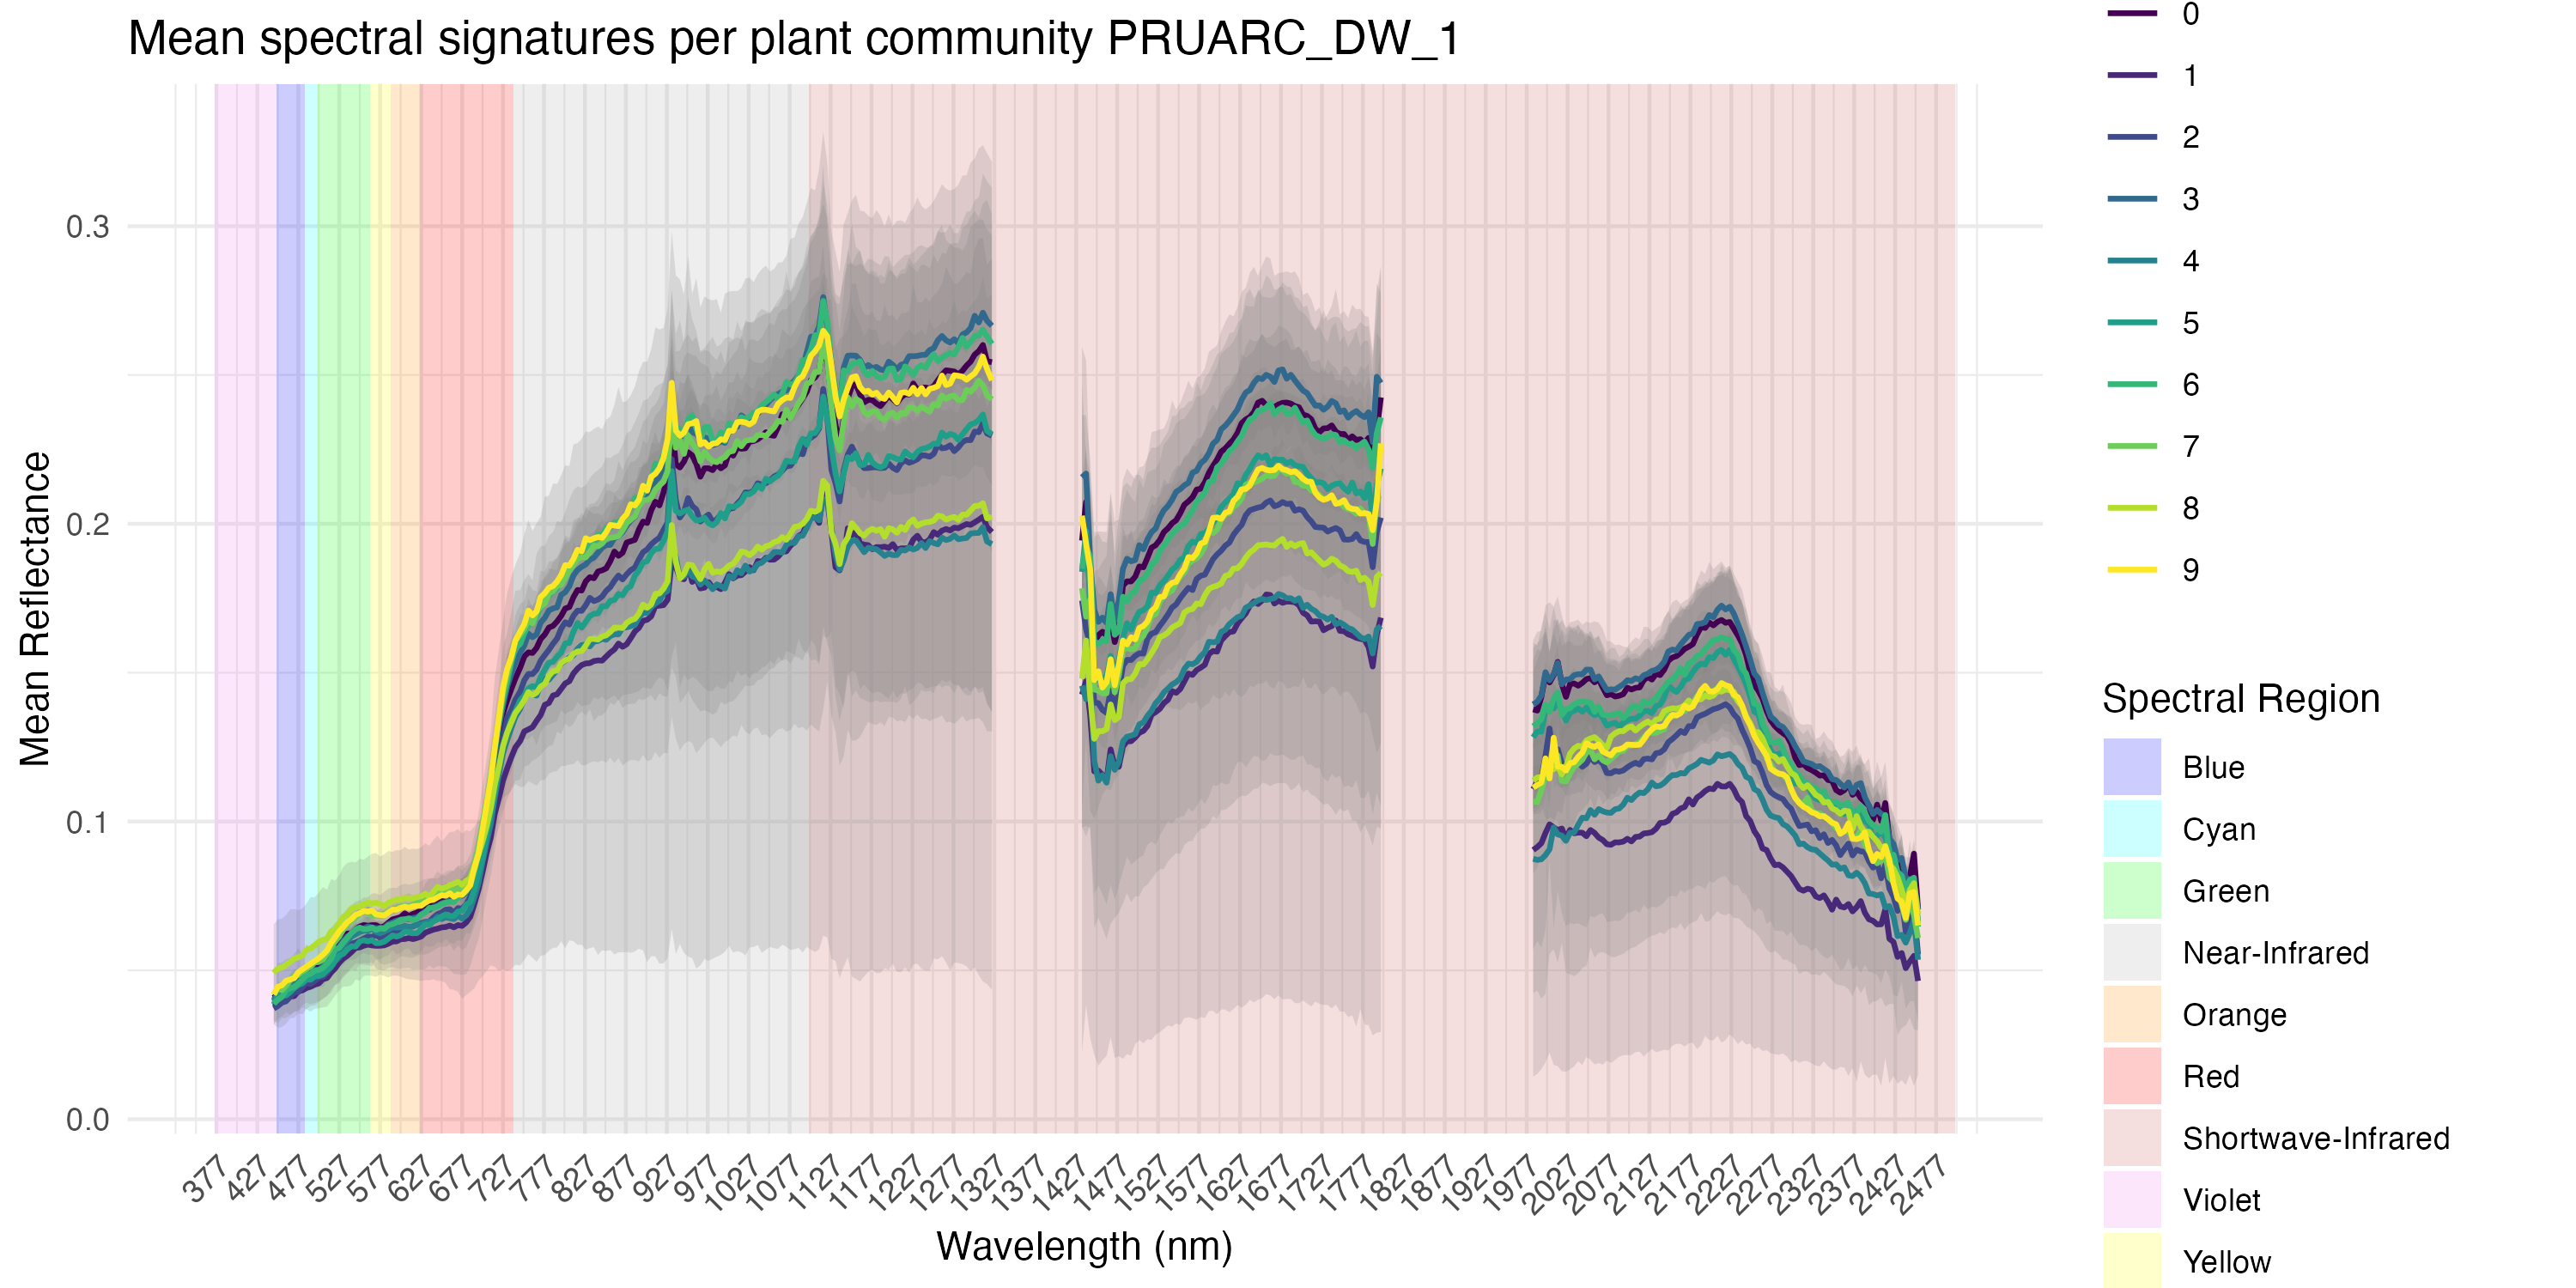
\includegraphics[width=\textwidth]{Figures/spectral_signatures/PRUARC_DW_1_mean_signature_plot_plant_community.png}
    \caption{}
    \label{fig:mss_pc_pruarcdw1}
  \end{subfigure}

  \caption{Spectral signature plot \ref{fig:ss_pc_pruarcdw1} and mean spectral signature plot \ref{fig:mss_pc_pruarcdw1} grouped by plant community cluster for test site PRUARC\_DW\_1}
  \label{fig:group_pc_ht_pruarcdw1}
\end{figure}





\subsection{Combined test sites}
In this subsection, the spectral signature lines across all the test sites were plotted grouped by habitat type.

\begin{figure}[H]
    \centering
    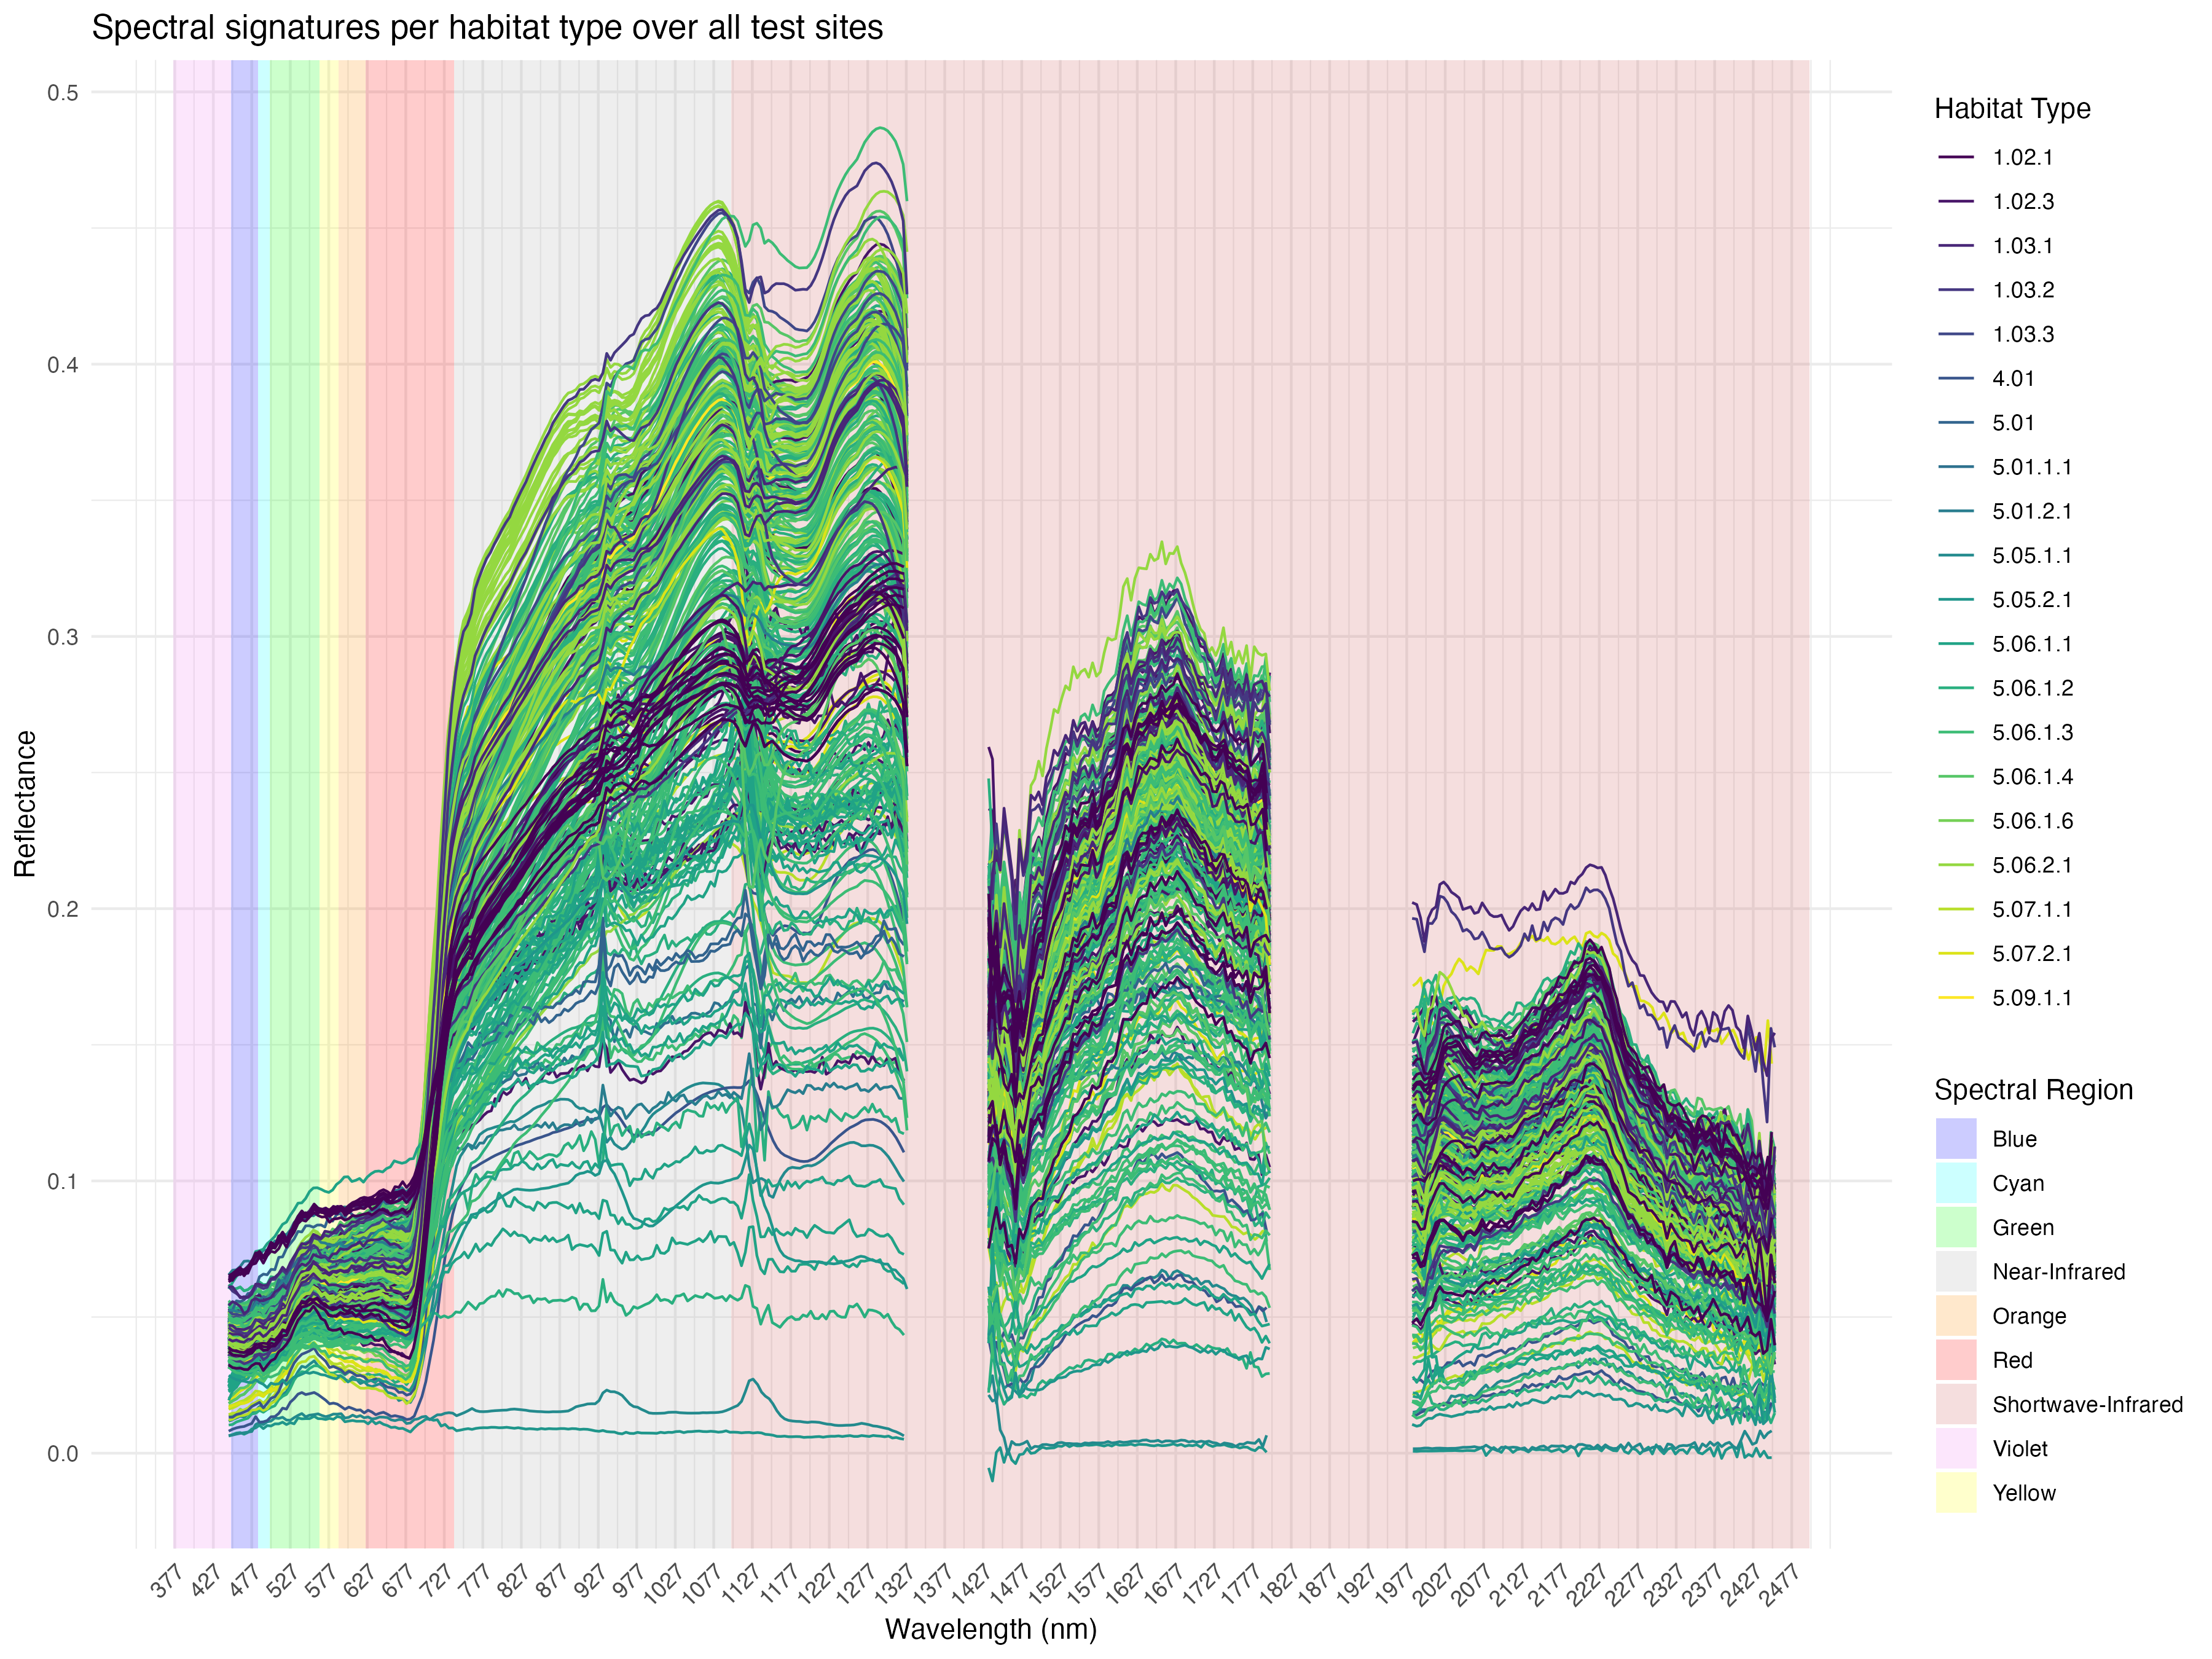
\includegraphics[width=0.9\textwidth]{Figures/spectral_signatures/All_testsites_signature_plot.png}
    \caption{The spectral signature plot over all the 354 test sites combined, grouped by habitat type}
    \label{fig:ss_all_testsites}
\end{figure}
